\documentclass[twoside]{book}

% Packages required by doxygen
\usepackage{fixltx2e}
\usepackage{calc}
\usepackage{doxygen}
\usepackage[export]{adjustbox} % also loads graphicx
\usepackage{graphicx}
\usepackage[utf8]{inputenc}
\usepackage{makeidx}
\usepackage{multicol}
\usepackage{multirow}
\PassOptionsToPackage{warn}{textcomp}
\usepackage{textcomp}
\usepackage[nointegrals]{wasysym}
\usepackage[table]{xcolor}

% Font selection
\usepackage[T1]{fontenc}
\usepackage[scaled=.90]{helvet}
\usepackage{courier}
\usepackage{amssymb}
\usepackage{sectsty}
\renewcommand{\familydefault}{\sfdefault}
\allsectionsfont{%
  \fontseries{bc}\selectfont%
  \color{darkgray}%
}
\renewcommand{\DoxyLabelFont}{%
  \fontseries{bc}\selectfont%
  \color{darkgray}%
}
\newcommand{\+}{\discretionary{\mbox{\scriptsize$\hookleftarrow$}}{}{}}

% Page & text layout
\usepackage{geometry}
\geometry{%
  a4paper,%
  top=2.5cm,%
  bottom=2.5cm,%
  left=2.5cm,%
  right=2.5cm%
}
\tolerance=750
\hfuzz=15pt
\hbadness=750
\setlength{\emergencystretch}{15pt}
\setlength{\parindent}{0cm}
\setlength{\parskip}{3ex plus 2ex minus 2ex}
\makeatletter
\renewcommand{\paragraph}{%
  \@startsection{paragraph}{4}{0ex}{-1.0ex}{1.0ex}{%
    \normalfont\normalsize\bfseries\SS@parafont%
  }%
}
\renewcommand{\subparagraph}{%
  \@startsection{subparagraph}{5}{0ex}{-1.0ex}{1.0ex}{%
    \normalfont\normalsize\bfseries\SS@subparafont%
  }%
}
\makeatother

% Headers & footers
\usepackage{fancyhdr}
\pagestyle{fancyplain}
\fancyhead[LE]{\fancyplain{}{\bfseries\thepage}}
\fancyhead[CE]{\fancyplain{}{}}
\fancyhead[RE]{\fancyplain{}{\bfseries\leftmark}}
\fancyhead[LO]{\fancyplain{}{\bfseries\rightmark}}
\fancyhead[CO]{\fancyplain{}{}}
\fancyhead[RO]{\fancyplain{}{\bfseries\thepage}}
\fancyfoot[LE]{\fancyplain{}{}}
\fancyfoot[CE]{\fancyplain{}{}}
\fancyfoot[RE]{\fancyplain{}{\bfseries\scriptsize Generated by Doxygen }}
\fancyfoot[LO]{\fancyplain{}{\bfseries\scriptsize Generated by Doxygen }}
\fancyfoot[CO]{\fancyplain{}{}}
\fancyfoot[RO]{\fancyplain{}{}}
\renewcommand{\footrulewidth}{0.4pt}
\renewcommand{\chaptermark}[1]{%
  \markboth{#1}{}%
}
\renewcommand{\sectionmark}[1]{%
  \markright{\thesection\ #1}%
}

% Indices & bibliography
\usepackage{natbib}
\usepackage[titles]{tocloft}
\setcounter{tocdepth}{3}
\setcounter{secnumdepth}{5}
\makeindex

% Hyperlinks (required, but should be loaded last)
\usepackage{ifpdf}
\ifpdf
  \usepackage[pdftex,pagebackref=true]{hyperref}
\else
  \usepackage[ps2pdf,pagebackref=true]{hyperref}
\fi
\hypersetup{%
  colorlinks=true,%
  linkcolor=blue,%
  citecolor=blue,%
  unicode%
}

% Custom commands
\newcommand{\clearemptydoublepage}{%
  \newpage{\pagestyle{empty}\cleardoublepage}%
}

\usepackage{caption}
\captionsetup{labelsep=space,justification=centering,font={bf},singlelinecheck=off,skip=4pt,position=top}

%===== C O N T E N T S =====

\begin{document}

% Titlepage & ToC
\hypersetup{pageanchor=false,
             bookmarksnumbered=true,
             pdfencoding=unicode
            }
\pagenumbering{roman}
\begin{titlepage}
\vspace*{7cm}
\begin{center}%
{\Large My Project }\\
\vspace*{1cm}
{\large Generated by Doxygen 1.8.11}\\
\end{center}
\end{titlepage}
\clearemptydoublepage
\tableofcontents
\clearemptydoublepage
\pagenumbering{arabic}
\hypersetup{pageanchor=true}

%--- Begin generated contents ---
\chapter{Module Index}
\section{Modules}
Here is a list of all modules\+:\begin{DoxyCompactList}
\item \contentsline{section}{Bike}{\pageref{group__Bike}}{}
\item \contentsline{section}{i8042}{\pageref{group__i8042}}{}
\item \contentsline{section}{i8254}{\pageref{group__i8254}}{}
\item \contentsline{section}{Keyboard}{\pageref{group__Keyboard}}{}
\item \contentsline{section}{lmlib}{\pageref{group__lmlib}}{}
\item \contentsline{section}{Menu}{\pageref{group__Menu}}{}
\item \contentsline{section}{Mouse}{\pageref{group__Mouse}}{}
\item \contentsline{section}{timer}{\pageref{group__timer}}{}
\item \contentsline{section}{vbe}{\pageref{group__vbe}}{}
\item \contentsline{section}{video\+\_\+gr}{\pageref{group__video__gr}}{}
\end{DoxyCompactList}

\chapter{Class Index}
\section{Class List}
Here are the classes, structs, unions and interfaces with brief descriptions\+:\begin{DoxyCompactList}
\item\contentsline{section}{\hyperlink{struct____attribute____}{\+\_\+\+\_\+attribute\+\_\+\+\_\+} }{\pageref{struct____attribute____}}{}
\item\contentsline{section}{\hyperlink{structBike}{Bike} }{\pageref{structBike}}{}
\item\contentsline{section}{\hyperlink{structMenu}{Menu} }{\pageref{structMenu}}{}
\item\contentsline{section}{\hyperlink{structmmap__t}{mmap\+\_\+t} }{\pageref{structmmap__t}}{}
\item\contentsline{section}{\hyperlink{structMouse}{Mouse} }{\pageref{structMouse}}{}
\item\contentsline{section}{\hyperlink{structstbi__io__callbacks}{stbi\+\_\+io\+\_\+callbacks} }{\pageref{structstbi__io__callbacks}}{}
\end{DoxyCompactList}

\chapter{File Index}
\section{File List}
Here is a list of all files with brief descriptions\+:\begin{DoxyCompactList}
\item\contentsline{section}{\hyperlink{bike_8c}{bike.\+c} }{\pageref{bike_8c}}{}
\item\contentsline{section}{\hyperlink{bike_8h}{bike.\+h} }{\pageref{bike_8h}}{}
\item\contentsline{section}{\hyperlink{i8042_8h}{i8042.\+h} }{\pageref{i8042_8h}}{}
\item\contentsline{section}{\hyperlink{i8254_8h}{i8254.\+h} }{\pageref{i8254_8h}}{}
\item\contentsline{section}{\hyperlink{keyboard_8c}{keyboard.\+c} }{\pageref{keyboard_8c}}{}
\item\contentsline{section}{\hyperlink{keyboard_8h}{keyboard.\+h} }{\pageref{keyboard_8h}}{}
\item\contentsline{section}{\hyperlink{lmlib_8h}{lmlib.\+h} }{\pageref{lmlib_8h}}{}
\item\contentsline{section}{\hyperlink{main_8c}{main.\+c} }{\pageref{main_8c}}{}
\item\contentsline{section}{\hyperlink{mainMenu_8c}{main\+Menu.\+c} }{\pageref{mainMenu_8c}}{}
\item\contentsline{section}{\hyperlink{mainMenu_8h}{main\+Menu.\+h} }{\pageref{mainMenu_8h}}{}
\item\contentsline{section}{\hyperlink{menu_8c}{menu.\+c} }{\pageref{menu_8c}}{}
\item\contentsline{section}{\hyperlink{menu_8h}{menu.\+h} }{\pageref{menu_8h}}{}
\item\contentsline{section}{\hyperlink{mouse_8c}{mouse.\+c} }{\pageref{mouse_8c}}{}
\item\contentsline{section}{\hyperlink{mouse_8h}{mouse.\+h} }{\pageref{mouse_8h}}{}
\item\contentsline{section}{\hyperlink{stb__image_8h}{stb\+\_\+image.\+h} }{\pageref{stb__image_8h}}{}
\item\contentsline{section}{\hyperlink{stbi__wrapper_8c}{stbi\+\_\+wrapper.\+c} }{\pageref{stbi__wrapper_8c}}{}
\item\contentsline{section}{\hyperlink{stbi__wrapper_8h}{stbi\+\_\+wrapper.\+h} }{\pageref{stbi__wrapper_8h}}{}
\item\contentsline{section}{\hyperlink{timer_8c}{timer.\+c} }{\pageref{timer_8c}}{}
\item\contentsline{section}{\hyperlink{timer_8h}{timer.\+h} }{\pageref{timer_8h}}{}
\item\contentsline{section}{\hyperlink{tron_8c}{tron.\+c} }{\pageref{tron_8c}}{}
\item\contentsline{section}{\hyperlink{tron_8h}{tron.\+h} }{\pageref{tron_8h}}{}
\item\contentsline{section}{\hyperlink{vbe_8c}{vbe.\+c} }{\pageref{vbe_8c}}{}
\item\contentsline{section}{\hyperlink{vbe_8h}{vbe.\+h} }{\pageref{vbe_8h}}{}
\item\contentsline{section}{\hyperlink{video_8h}{video.\+h} }{\pageref{video_8h}}{}
\item\contentsline{section}{\hyperlink{video__gr_8c}{video\+\_\+gr.\+c} }{\pageref{video__gr_8c}}{}
\item\contentsline{section}{\hyperlink{video__gr_8h}{video\+\_\+gr.\+h} }{\pageref{video__gr_8h}}{}
\end{DoxyCompactList}

\chapter{Module Documentation}
\hypertarget{group__Bike}{}\section{Bike}
\label{group__Bike}\index{Bike@{Bike}}
\subsection*{Classes}
\begin{DoxyCompactItemize}
\item 
struct \hyperlink{structBike}{Bike}
\end{DoxyCompactItemize}
\subsection*{Typedefs}
\begin{DoxyCompactItemize}
\item 
typedef struct \hyperlink{structBike}{Bike} \hyperlink{group__Bike_ga85f4cbf9698a8ed38ad74f4e2d71341e}{Bike}
\end{DoxyCompactItemize}
\subsection*{Functions}
\begin{DoxyCompactItemize}
\item 
int \hyperlink{group__Bike_ga9d5bd9dd5a4b9347fa04fb0a47e7b138}{get\+InitialX} (struct \hyperlink{structBike}{Bike} bike)
\begin{DoxyCompactList}\small\item\em gets Initial X position \end{DoxyCompactList}\item 
int \hyperlink{group__Bike_ga2d556c34524f8fe950a96aa665aaffe8}{get\+InitialY} (struct \hyperlink{structBike}{Bike} bike)
\begin{DoxyCompactList}\small\item\em gets Initial Y position \end{DoxyCompactList}\item 
int \hyperlink{group__Bike_ga8d48f7de63dc2a17f3eac8b3e96f9b12}{get\+Direction} (struct \hyperlink{structBike}{Bike} bike)
\begin{DoxyCompactList}\small\item\em gets bike direction \end{DoxyCompactList}\item 
int \hyperlink{group__Bike_gaf4691615a2b7398e9c3b4ae2f93553e0}{get\+HeadX} (struct \hyperlink{structBike}{Bike} bike)
\begin{DoxyCompactList}\small\item\em gets Head X position \end{DoxyCompactList}\item 
int \hyperlink{group__Bike_gaafe273e5e247e3efd463e232686328d6}{get\+HeadY} (struct \hyperlink{structBike}{Bike} bike)
\begin{DoxyCompactList}\small\item\em gets Head Y position \end{DoxyCompactList}\item 
unsigned long \hyperlink{group__Bike_ga04fad9ee3b40712d1fde03fc5441ea73}{getcolor} (struct \hyperlink{structBike}{Bike} bike)
\begin{DoxyCompactList}\small\item\em gets the bike color \end{DoxyCompactList}\item 
void \hyperlink{group__Bike_ga0310311d1c88668900502c150b52120b}{set\+Direction} (\hyperlink{structBike}{Bike} $\ast$bike, int dir)
\begin{DoxyCompactList}\small\item\em sets the bike direction \end{DoxyCompactList}\item 
void \hyperlink{group__Bike_gadd2170ef6cbb83a919f06cf9c971c9a5}{move\+Head} (\hyperlink{structBike}{Bike} $\ast$bike, int speed)
\begin{DoxyCompactList}\small\item\em gets the bike color \end{DoxyCompactList}\end{DoxyCompactItemize}
\subsection*{Variables}
\begin{DoxyCompactItemize}
\item 
int \hyperlink{group__Bike_ga01cdf583ace46bc4e576c42b54ee628a}{Bike\+::initial\+\_\+x\+\_\+pos}
\item 
int \hyperlink{group__Bike_ga74f0f95635444a7570225a75f3a22056}{Bike\+::initial\+\_\+y\+\_\+pos}
\item 
int \hyperlink{group__Bike_ga9a5251a8d520f2ce0fc0e34dd7325a23}{Bike\+::direction}
\item 
int \hyperlink{group__Bike_ga3187c35b871d499fb88aca98de35282a}{Bike\+::head\+\_\+x\+\_\+pos}
\item 
int \hyperlink{group__Bike_ga48e90acd4f7eceb4ea0921f9a8b89f98}{Bike\+::head\+\_\+y\+\_\+pos}
\item 
unsigned long \hyperlink{group__Bike_ga7ba066e0787d8b239b8cb16775db0eac}{Bike\+::color}
\end{DoxyCompactItemize}


\subsection{Detailed Description}
\hyperlink{structBike}{Bike} Struct Functions to manipulate the bike 

\subsection{Typedef Documentation}
\index{Bike@{Bike}!Bike@{Bike}}
\index{Bike@{Bike}!Bike@{Bike}}
\subsubsection[{\texorpdfstring{Bike}{Bike}}]{\setlength{\rightskip}{0pt plus 5cm}typedef struct {\bf Bike}  {\bf Bike}}\hypertarget{group__Bike_ga85f4cbf9698a8ed38ad74f4e2d71341e}{}\label{group__Bike_ga85f4cbf9698a8ed38ad74f4e2d71341e}


\subsection{Function Documentation}
\index{Bike@{Bike}!getcolor@{getcolor}}
\index{getcolor@{getcolor}!Bike@{Bike}}
\subsubsection[{\texorpdfstring{getcolor(struct Bike bike)}{getcolor(struct Bike bike)}}]{\setlength{\rightskip}{0pt plus 5cm}unsigned long getcolor (
\begin{DoxyParamCaption}
\item[{struct {\bf Bike}}]{bike}
\end{DoxyParamCaption}
)}\hypertarget{group__Bike_ga04fad9ee3b40712d1fde03fc5441ea73}{}\label{group__Bike_ga04fad9ee3b40712d1fde03fc5441ea73}


gets the bike color 


\begin{DoxyParams}{Parameters}
{\em bike} & the bike struct\\
\hline
\end{DoxyParams}
\begin{DoxyReturn}{Returns}
bike color 
\end{DoxyReturn}
\index{Bike@{Bike}!get\+Direction@{get\+Direction}}
\index{get\+Direction@{get\+Direction}!Bike@{Bike}}
\subsubsection[{\texorpdfstring{get\+Direction(struct Bike bike)}{getDirection(struct Bike bike)}}]{\setlength{\rightskip}{0pt plus 5cm}int get\+Direction (
\begin{DoxyParamCaption}
\item[{struct {\bf Bike}}]{bike}
\end{DoxyParamCaption}
)}\hypertarget{group__Bike_ga8d48f7de63dc2a17f3eac8b3e96f9b12}{}\label{group__Bike_ga8d48f7de63dc2a17f3eac8b3e96f9b12}


gets bike direction 


\begin{DoxyParams}{Parameters}
{\em bike} & the bike struct\\
\hline
\end{DoxyParams}
\begin{DoxyReturn}{Returns}
bike direction 
\end{DoxyReturn}
\index{Bike@{Bike}!get\+HeadX@{get\+HeadX}}
\index{get\+HeadX@{get\+HeadX}!Bike@{Bike}}
\subsubsection[{\texorpdfstring{get\+Head\+X(struct Bike bike)}{getHeadX(struct Bike bike)}}]{\setlength{\rightskip}{0pt plus 5cm}int get\+HeadX (
\begin{DoxyParamCaption}
\item[{struct {\bf Bike}}]{bike}
\end{DoxyParamCaption}
)}\hypertarget{group__Bike_gaf4691615a2b7398e9c3b4ae2f93553e0}{}\label{group__Bike_gaf4691615a2b7398e9c3b4ae2f93553e0}


gets Head X position 


\begin{DoxyParams}{Parameters}
{\em bike} & the bike struct\\
\hline
\end{DoxyParams}
\begin{DoxyReturn}{Returns}
bike Head X position 
\end{DoxyReturn}
\index{Bike@{Bike}!get\+HeadY@{get\+HeadY}}
\index{get\+HeadY@{get\+HeadY}!Bike@{Bike}}
\subsubsection[{\texorpdfstring{get\+Head\+Y(struct Bike bike)}{getHeadY(struct Bike bike)}}]{\setlength{\rightskip}{0pt plus 5cm}int get\+HeadY (
\begin{DoxyParamCaption}
\item[{struct {\bf Bike}}]{bike}
\end{DoxyParamCaption}
)}\hypertarget{group__Bike_gaafe273e5e247e3efd463e232686328d6}{}\label{group__Bike_gaafe273e5e247e3efd463e232686328d6}


gets Head Y position 


\begin{DoxyParams}{Parameters}
{\em bike} & the bike struct\\
\hline
\end{DoxyParams}
\begin{DoxyReturn}{Returns}
bike Head Y position 
\end{DoxyReturn}
\index{Bike@{Bike}!get\+InitialX@{get\+InitialX}}
\index{get\+InitialX@{get\+InitialX}!Bike@{Bike}}
\subsubsection[{\texorpdfstring{get\+Initial\+X(struct Bike bike)}{getInitialX(struct Bike bike)}}]{\setlength{\rightskip}{0pt plus 5cm}int get\+InitialX (
\begin{DoxyParamCaption}
\item[{struct {\bf Bike}}]{bike}
\end{DoxyParamCaption}
)}\hypertarget{group__Bike_ga9d5bd9dd5a4b9347fa04fb0a47e7b138}{}\label{group__Bike_ga9d5bd9dd5a4b9347fa04fb0a47e7b138}


gets Initial X position 


\begin{DoxyParams}{Parameters}
{\em bike} & the bike struct\\
\hline
\end{DoxyParams}
\begin{DoxyReturn}{Returns}
bike initial X position 
\end{DoxyReturn}
\index{Bike@{Bike}!get\+InitialY@{get\+InitialY}}
\index{get\+InitialY@{get\+InitialY}!Bike@{Bike}}
\subsubsection[{\texorpdfstring{get\+Initial\+Y(struct Bike bike)}{getInitialY(struct Bike bike)}}]{\setlength{\rightskip}{0pt plus 5cm}int get\+InitialY (
\begin{DoxyParamCaption}
\item[{struct {\bf Bike}}]{bike}
\end{DoxyParamCaption}
)}\hypertarget{group__Bike_ga2d556c34524f8fe950a96aa665aaffe8}{}\label{group__Bike_ga2d556c34524f8fe950a96aa665aaffe8}


gets Initial Y position 


\begin{DoxyParams}{Parameters}
{\em bike} & the bike struct\\
\hline
\end{DoxyParams}
\begin{DoxyReturn}{Returns}
bike initial Y position 
\end{DoxyReturn}
\index{Bike@{Bike}!move\+Head@{move\+Head}}
\index{move\+Head@{move\+Head}!Bike@{Bike}}
\subsubsection[{\texorpdfstring{move\+Head(\+Bike $\ast$bike, int speed)}{moveHead(Bike *bike, int speed)}}]{\setlength{\rightskip}{0pt plus 5cm}void move\+Head (
\begin{DoxyParamCaption}
\item[{{\bf Bike} $\ast$}]{bike, }
\item[{int}]{speed}
\end{DoxyParamCaption}
)}\hypertarget{group__Bike_gadd2170ef6cbb83a919f06cf9c971c9a5}{}\label{group__Bike_gadd2170ef6cbb83a919f06cf9c971c9a5}


gets the bike color 


\begin{DoxyParams}{Parameters}
{\em bike} & the bike object\\
\hline
{\em speed} & the bike speed \\
\hline
\end{DoxyParams}


Here is the call graph for this function\+:
\nopagebreak
\begin{figure}[H]
\begin{center}
\leavevmode
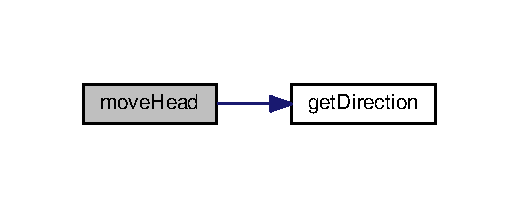
\includegraphics[width=249pt]{group__Bike_gadd2170ef6cbb83a919f06cf9c971c9a5_cgraph}
\end{center}
\end{figure}


\index{Bike@{Bike}!set\+Direction@{set\+Direction}}
\index{set\+Direction@{set\+Direction}!Bike@{Bike}}
\subsubsection[{\texorpdfstring{set\+Direction(\+Bike $\ast$bike, int dir)}{setDirection(Bike *bike, int dir)}}]{\setlength{\rightskip}{0pt plus 5cm}void set\+Direction (
\begin{DoxyParamCaption}
\item[{{\bf Bike} $\ast$}]{bike, }
\item[{int}]{dir}
\end{DoxyParamCaption}
)}\hypertarget{group__Bike_ga0310311d1c88668900502c150b52120b}{}\label{group__Bike_ga0310311d1c88668900502c150b52120b}


sets the bike direction 


\begin{DoxyParams}{Parameters}
{\em bike} & the bike object\\
\hline
{\em dir} & the bike direction \\
\hline
\end{DoxyParams}


\subsection{Variable Documentation}
\index{Bike@{Bike}!color@{color}}
\index{color@{color}!Bike@{Bike}}
\subsubsection[{\texorpdfstring{color}{color}}]{\setlength{\rightskip}{0pt plus 5cm}unsigned long Bike\+::color}\hypertarget{group__Bike_ga7ba066e0787d8b239b8cb16775db0eac}{}\label{group__Bike_ga7ba066e0787d8b239b8cb16775db0eac}
bike color \index{Bike@{Bike}!direction@{direction}}
\index{direction@{direction}!Bike@{Bike}}
\subsubsection[{\texorpdfstring{direction}{direction}}]{\setlength{\rightskip}{0pt plus 5cm}int Bike\+::direction}\hypertarget{group__Bike_ga9a5251a8d520f2ce0fc0e34dd7325a23}{}\label{group__Bike_ga9a5251a8d520f2ce0fc0e34dd7325a23}
direction \index{Bike@{Bike}!head\+\_\+x\+\_\+pos@{head\+\_\+x\+\_\+pos}}
\index{head\+\_\+x\+\_\+pos@{head\+\_\+x\+\_\+pos}!Bike@{Bike}}
\subsubsection[{\texorpdfstring{head\+\_\+x\+\_\+pos}{head_x_pos}}]{\setlength{\rightskip}{0pt plus 5cm}int Bike\+::head\+\_\+x\+\_\+pos}\hypertarget{group__Bike_ga3187c35b871d499fb88aca98de35282a}{}\label{group__Bike_ga3187c35b871d499fb88aca98de35282a}
head X position \index{Bike@{Bike}!head\+\_\+y\+\_\+pos@{head\+\_\+y\+\_\+pos}}
\index{head\+\_\+y\+\_\+pos@{head\+\_\+y\+\_\+pos}!Bike@{Bike}}
\subsubsection[{\texorpdfstring{head\+\_\+y\+\_\+pos}{head_y_pos}}]{\setlength{\rightskip}{0pt plus 5cm}int Bike\+::head\+\_\+y\+\_\+pos}\hypertarget{group__Bike_ga48e90acd4f7eceb4ea0921f9a8b89f98}{}\label{group__Bike_ga48e90acd4f7eceb4ea0921f9a8b89f98}
head Y position \index{Bike@{Bike}!initial\+\_\+x\+\_\+pos@{initial\+\_\+x\+\_\+pos}}
\index{initial\+\_\+x\+\_\+pos@{initial\+\_\+x\+\_\+pos}!Bike@{Bike}}
\subsubsection[{\texorpdfstring{initial\+\_\+x\+\_\+pos}{initial_x_pos}}]{\setlength{\rightskip}{0pt plus 5cm}int Bike\+::initial\+\_\+x\+\_\+pos}\hypertarget{group__Bike_ga01cdf583ace46bc4e576c42b54ee628a}{}\label{group__Bike_ga01cdf583ace46bc4e576c42b54ee628a}
initial X position \index{Bike@{Bike}!initial\+\_\+y\+\_\+pos@{initial\+\_\+y\+\_\+pos}}
\index{initial\+\_\+y\+\_\+pos@{initial\+\_\+y\+\_\+pos}!Bike@{Bike}}
\subsubsection[{\texorpdfstring{initial\+\_\+y\+\_\+pos}{initial_y_pos}}]{\setlength{\rightskip}{0pt plus 5cm}int Bike\+::initial\+\_\+y\+\_\+pos}\hypertarget{group__Bike_ga74f0f95635444a7570225a75f3a22056}{}\label{group__Bike_ga74f0f95635444a7570225a75f3a22056}
initial Y position 
\hypertarget{group__i8042}{}\section{i8042}
\label{group__i8042}\index{i8042@{i8042}}
\subsection*{Macros}
\begin{DoxyCompactItemize}
\item 
\#define \hyperlink{group__i8042_ga3a8ea58898cb58fc96013383d39f482c}{B\+IT}(n)~(0x01$<$$<$(n))
\item 
\#define \hyperlink{group__i8042_ga1a522aa19bcb695a9df30032a893bee3}{D\+E\+L\+A\+Y\+\_\+\+US}~20000
\item 
\#define \hyperlink{group__i8042_ga45ba202b05caf39795aeca91b0ae547e}{T\+I\+M\+E\+O\+UT}~4
\item 
\#define \hyperlink{group__i8042_ga16c5827f043d82f87c726c2d4369c11d}{K\+B\+C\+\_\+\+I\+RQ}~1
\begin{DoxyCompactList}\small\item\em K\+BC I\+RQ line. \end{DoxyCompactList}\item 
\#define \hyperlink{group__i8042_ga85964cb90343bb1a029b1d1b4229f910}{M\+O\+U\+S\+E\+\_\+\+I\+RQ}~12
\item 
\#define \hyperlink{group__i8042_ga89c4d098b53809674457b1660b1af780}{S\+T\+A\+T\+\_\+\+R\+EG}~0x64
\item 
\#define \hyperlink{group__i8042_ga6d57c7927a10f638c83046b52c8caac9}{K\+B\+C\+\_\+\+C\+M\+D\+\_\+\+R\+EG}~0x64
\item 
\#define \hyperlink{group__i8042_gacfb42dde389e8ca36ab267002fbf5c6a}{O\+U\+T\+\_\+\+B\+UF}~0x60
\item 
\#define \hyperlink{group__i8042_ga783be5698cf07b1daaf126ef89c19063}{I\+N\+\_\+\+B\+UF}~0x60
\item 
\#define \hyperlink{group__i8042_ga45967c9e25447ba853cf6fb4ac545fe6}{O\+BF}~\hyperlink{video_8h_a3a8ea58898cb58fc96013383d39f482c}{B\+IT}(0)
\item 
\#define \hyperlink{group__i8042_ga3c48b10907056351582baf9f6478598e}{I\+BF}~\hyperlink{video_8h_a3a8ea58898cb58fc96013383d39f482c}{B\+IT}(1)
\item 
\#define \hyperlink{group__i8042_ga307ab71673e26ec42b28a3bca05d4cb5}{P\+A\+R\+\_\+\+E\+RR}~\hyperlink{video_8h_a3a8ea58898cb58fc96013383d39f482c}{B\+IT}(7)
\item 
\#define \hyperlink{group__i8042_gad16f61e2bf70f6c7685e826224ed177f}{T\+O\+\_\+\+E\+RR}~\hyperlink{video_8h_a3a8ea58898cb58fc96013383d39f482c}{B\+IT}(6)
\item 
\#define \hyperlink{group__i8042_gad6ff09b5058171ce69f6485dbef6bfaa}{B\+R\+E\+A\+K\+C\+O\+DE}~\hyperlink{video_8h_a3a8ea58898cb58fc96013383d39f482c}{B\+IT}(7)
\item 
\#define \hyperlink{group__i8042_ga77c789e6ff7b6f33ac32ba84d3983ca4}{B\+R\+E\+A\+K\+C\+O\+D\+E\+\_\+\+E\+SC}~0x81
\item 
\#define \hyperlink{group__i8042_gab9da23ad538a1a1a68466865ac73f9b8}{T\+O\+W\+\_\+\+B\+Y\+T\+E\+\_\+\+C\+O\+DE}~0x\+E0
\item 
\#define \hyperlink{group__i8042_gaa7a45554686b9abe54443a4a80e8d2f5}{M\+A\+K\+E\+C\+O\+D\+E\+\_\+A}~0x1E
\item 
\#define \hyperlink{group__i8042_ga48a460d951bb61b2aa11903c8e817b6c}{M\+A\+K\+E\+C\+O\+D\+E\+\_\+W}~0x11
\item 
\#define \hyperlink{group__i8042_ga248870237f8cc9a4e73683480d2cfae3}{M\+A\+K\+E\+C\+O\+D\+E\+\_\+S}~0x1F
\item 
\#define \hyperlink{group__i8042_ga2c181b340e0f7986f6ea695164558fc8}{M\+A\+K\+E\+C\+O\+D\+E\+\_\+D}~0x20
\item 
\#define \hyperlink{group__i8042_ga2a701bb9a46d001c52ff40857c50daf1}{M\+A\+K\+E\+C\+O\+D\+E\+\_\+\+U\+P\+\_\+\+N\+U\+M\+P\+A\+D8}~0x48
\item 
\#define \hyperlink{group__i8042_ga820a37037cac38b3147934bdbe601843}{M\+A\+K\+E\+C\+O\+D\+E\+\_\+\+L\+E\+F\+T\+\_\+\+N\+U\+M\+P\+A\+D4}~0x4B
\item 
\#define \hyperlink{group__i8042_ga58501b39296e524f307c139e2b13b77e}{M\+A\+K\+E\+C\+O\+D\+E\+\_\+\+D\+O\+W\+N\+\_\+\+N\+U\+M\+P\+A\+D2}~0x50
\item 
\#define \hyperlink{group__i8042_gac8a539e1de5071da15f4cd6f94aba242}{M\+A\+K\+E\+C\+O\+D\+E\+\_\+\+R\+I\+G\+H\+T\+\_\+\+N\+U\+M\+P\+A\+D6}~0x4D
\item 
\#define \hyperlink{group__i8042_ga305ee86129081b404b151c64293566e7}{R\+E\+A\+D\+\_\+\+C\+O\+M\+M\+A\+N\+D\+\_\+\+B\+Y\+TE}~0x20
\item 
\#define \hyperlink{group__i8042_ga4680153f26a3244682a2e2e01e57e318}{W\+R\+I\+T\+E\+\_\+\+C\+O\+M\+M\+A\+N\+D\+\_\+\+B\+Y\+TE}~0x60
\item 
\#define \hyperlink{group__i8042_ga11095772a492a95192ea75373df94b65}{B\+Y\+T\+E\+\_\+\+T\+O\+\_\+\+M\+O\+U\+SE}~0x\+D4
\item 
\#define \hyperlink{group__i8042_gae70fc1a5ba1238a43c0f5b07740ab438}{E\+N\+A\+B\+L\+E\+\_\+\+M\+O\+U\+S\+E\+\_\+\+I\+NT}~0x47
\item 
\#define \hyperlink{group__i8042_ga1c22608f41bd715500d0333001079a8a}{E\+N\+A\+B\+L\+E\+\_\+\+D\+A\+T\+A\+\_\+\+R\+E\+P\+O\+RT}~0x\+F4
\item 
\#define \hyperlink{group__i8042_gad374b510092499b5961d3771abf9c66e}{D\+I\+S\+A\+B\+L\+E\+\_\+\+D\+A\+T\+A\+\_\+\+R\+E\+P\+O\+RT}~0x\+F5
\item 
\#define \hyperlink{group__i8042_gaabf49b4a4d8ad72d202c8a7197058e35}{S\+E\+T\+\_\+\+S\+T\+R\+E\+A\+M\+\_\+\+M\+O\+DE}~0x\+EA
\item 
\#define \hyperlink{group__i8042_ga19a57d9d2eafd32ee130c0f526906719}{S\+E\+T\+\_\+\+R\+E\+M\+O\+T\+E\+\_\+\+M\+O\+DE}~0x\+F0
\item 
\#define \hyperlink{group__i8042_ga8d406d5aff787991429e62cfd9bac721}{R\+E\+A\+D\+\_\+\+D\+A\+TA}~0x\+EB
\item 
\#define \hyperlink{group__i8042_ga6f6489887e08bff4887d0bc5dcf214d8}{A\+CK}~0x\+FA
\item 
\#define \hyperlink{group__i8042_ga958518a45b12053ae33606ee7cb68a55}{N\+A\+CK}~0x\+FE
\item 
\#define \hyperlink{group__i8042_ga8fe83ac76edc595f6b98cd4a4127aed5}{E\+R\+R\+OR}~0x\+FC
\item 
\#define \hyperlink{group__i8042_gacc55daa58d88a3612f2ef74a6abbe97f}{LB}~\hyperlink{video_8h_a3a8ea58898cb58fc96013383d39f482c}{B\+IT}(0)
\item 
\#define \hyperlink{group__i8042_ga171160a766f85c8816b898ed24d28408}{RB}~\hyperlink{video_8h_a3a8ea58898cb58fc96013383d39f482c}{B\+IT}(1)
\item 
\#define \hyperlink{group__i8042_gaa6b38d492364d98453284934ed7caee9}{MB}~\hyperlink{video_8h_a3a8ea58898cb58fc96013383d39f482c}{B\+IT}(2)
\item 
\#define \hyperlink{group__i8042_ga22a4873e9adebfc22650f6776375cce6}{X\+S\+I\+GN}~\hyperlink{video_8h_a3a8ea58898cb58fc96013383d39f482c}{B\+IT}(4)
\item 
\#define \hyperlink{group__i8042_gaf4bf97e57d9aadf00d2ec881727cccef}{Y\+S\+I\+GN}~\hyperlink{video_8h_a3a8ea58898cb58fc96013383d39f482c}{B\+IT}(5)
\item 
\#define \hyperlink{group__i8042_gac3172c891b25dafed9ced2476aa03cf1}{X\+O\+VF}~\hyperlink{video_8h_a3a8ea58898cb58fc96013383d39f482c}{B\+IT}(6)
\item 
\#define \hyperlink{group__i8042_ga08deb639aef83c70892a364261b09133}{Y\+O\+VF}~\hyperlink{video_8h_a3a8ea58898cb58fc96013383d39f482c}{B\+IT}(7)
\item 
\#define \hyperlink{group__i8042_ga79d10e672abb49ad63eeaa8aaef57c38}{B\+L\+UE}~0x0B
\item 
\#define \hyperlink{group__i8042_ga87b537f5fa5c109d3c05c13d6b18f382}{W\+H\+I\+TE}~0x3F
\item 
\#define \hyperlink{group__i8042_ga1965eaca47dbf3f87acdafc2208f04eb}{UP}~1
\item 
\#define \hyperlink{group__i8042_ga80fb826a684cf3f0d306b22aa100ddac}{R\+I\+G\+HT}~2
\item 
\#define \hyperlink{group__i8042_ga4193cd1c8c2e6ebd0e056fa2364a663f}{D\+O\+WN}~3
\item 
\#define \hyperlink{group__i8042_ga437ef08681e7210d6678427030446a54}{L\+E\+FT}~4
\end{DoxyCompactItemize}


\subsection{Detailed Description}
Constants for programming the i8042 Key\+Board Controller. 

\subsection{Macro Definition Documentation}
\index{i8042@{i8042}!A\+CK@{A\+CK}}
\index{A\+CK@{A\+CK}!i8042@{i8042}}
\subsubsection[{\texorpdfstring{A\+CK}{ACK}}]{\setlength{\rightskip}{0pt plus 5cm}\#define A\+CK~0x\+FA}\hypertarget{group__i8042_ga6f6489887e08bff4887d0bc5dcf214d8}{}\label{group__i8042_ga6f6489887e08bff4887d0bc5dcf214d8}
\index{i8042@{i8042}!B\+IT@{B\+IT}}
\index{B\+IT@{B\+IT}!i8042@{i8042}}
\subsubsection[{\texorpdfstring{B\+IT}{BIT}}]{\setlength{\rightskip}{0pt plus 5cm}\#define B\+IT(
\begin{DoxyParamCaption}
\item[{}]{n}
\end{DoxyParamCaption}
)~(0x01$<$$<$(n))}\hypertarget{group__i8042_ga3a8ea58898cb58fc96013383d39f482c}{}\label{group__i8042_ga3a8ea58898cb58fc96013383d39f482c}
\index{i8042@{i8042}!B\+L\+UE@{B\+L\+UE}}
\index{B\+L\+UE@{B\+L\+UE}!i8042@{i8042}}
\subsubsection[{\texorpdfstring{B\+L\+UE}{BLUE}}]{\setlength{\rightskip}{0pt plus 5cm}\#define B\+L\+UE~0x0B}\hypertarget{group__i8042_ga79d10e672abb49ad63eeaa8aaef57c38}{}\label{group__i8042_ga79d10e672abb49ad63eeaa8aaef57c38}
\index{i8042@{i8042}!B\+R\+E\+A\+K\+C\+O\+DE@{B\+R\+E\+A\+K\+C\+O\+DE}}
\index{B\+R\+E\+A\+K\+C\+O\+DE@{B\+R\+E\+A\+K\+C\+O\+DE}!i8042@{i8042}}
\subsubsection[{\texorpdfstring{B\+R\+E\+A\+K\+C\+O\+DE}{BREAKCODE}}]{\setlength{\rightskip}{0pt plus 5cm}\#define B\+R\+E\+A\+K\+C\+O\+DE~{\bf B\+IT}(7)}\hypertarget{group__i8042_gad6ff09b5058171ce69f6485dbef6bfaa}{}\label{group__i8042_gad6ff09b5058171ce69f6485dbef6bfaa}
\index{i8042@{i8042}!B\+R\+E\+A\+K\+C\+O\+D\+E\+\_\+\+E\+SC@{B\+R\+E\+A\+K\+C\+O\+D\+E\+\_\+\+E\+SC}}
\index{B\+R\+E\+A\+K\+C\+O\+D\+E\+\_\+\+E\+SC@{B\+R\+E\+A\+K\+C\+O\+D\+E\+\_\+\+E\+SC}!i8042@{i8042}}
\subsubsection[{\texorpdfstring{B\+R\+E\+A\+K\+C\+O\+D\+E\+\_\+\+E\+SC}{BREAKCODE_ESC}}]{\setlength{\rightskip}{0pt plus 5cm}\#define B\+R\+E\+A\+K\+C\+O\+D\+E\+\_\+\+E\+SC~0x81}\hypertarget{group__i8042_ga77c789e6ff7b6f33ac32ba84d3983ca4}{}\label{group__i8042_ga77c789e6ff7b6f33ac32ba84d3983ca4}
\index{i8042@{i8042}!B\+Y\+T\+E\+\_\+\+T\+O\+\_\+\+M\+O\+U\+SE@{B\+Y\+T\+E\+\_\+\+T\+O\+\_\+\+M\+O\+U\+SE}}
\index{B\+Y\+T\+E\+\_\+\+T\+O\+\_\+\+M\+O\+U\+SE@{B\+Y\+T\+E\+\_\+\+T\+O\+\_\+\+M\+O\+U\+SE}!i8042@{i8042}}
\subsubsection[{\texorpdfstring{B\+Y\+T\+E\+\_\+\+T\+O\+\_\+\+M\+O\+U\+SE}{BYTE_TO_MOUSE}}]{\setlength{\rightskip}{0pt plus 5cm}\#define B\+Y\+T\+E\+\_\+\+T\+O\+\_\+\+M\+O\+U\+SE~0x\+D4}\hypertarget{group__i8042_ga11095772a492a95192ea75373df94b65}{}\label{group__i8042_ga11095772a492a95192ea75373df94b65}
\index{i8042@{i8042}!D\+E\+L\+A\+Y\+\_\+\+US@{D\+E\+L\+A\+Y\+\_\+\+US}}
\index{D\+E\+L\+A\+Y\+\_\+\+US@{D\+E\+L\+A\+Y\+\_\+\+US}!i8042@{i8042}}
\subsubsection[{\texorpdfstring{D\+E\+L\+A\+Y\+\_\+\+US}{DELAY_US}}]{\setlength{\rightskip}{0pt plus 5cm}\#define D\+E\+L\+A\+Y\+\_\+\+US~20000}\hypertarget{group__i8042_ga1a522aa19bcb695a9df30032a893bee3}{}\label{group__i8042_ga1a522aa19bcb695a9df30032a893bee3}
\index{i8042@{i8042}!D\+I\+S\+A\+B\+L\+E\+\_\+\+D\+A\+T\+A\+\_\+\+R\+E\+P\+O\+RT@{D\+I\+S\+A\+B\+L\+E\+\_\+\+D\+A\+T\+A\+\_\+\+R\+E\+P\+O\+RT}}
\index{D\+I\+S\+A\+B\+L\+E\+\_\+\+D\+A\+T\+A\+\_\+\+R\+E\+P\+O\+RT@{D\+I\+S\+A\+B\+L\+E\+\_\+\+D\+A\+T\+A\+\_\+\+R\+E\+P\+O\+RT}!i8042@{i8042}}
\subsubsection[{\texorpdfstring{D\+I\+S\+A\+B\+L\+E\+\_\+\+D\+A\+T\+A\+\_\+\+R\+E\+P\+O\+RT}{DISABLE_DATA_REPORT}}]{\setlength{\rightskip}{0pt plus 5cm}\#define D\+I\+S\+A\+B\+L\+E\+\_\+\+D\+A\+T\+A\+\_\+\+R\+E\+P\+O\+RT~0x\+F5}\hypertarget{group__i8042_gad374b510092499b5961d3771abf9c66e}{}\label{group__i8042_gad374b510092499b5961d3771abf9c66e}
\index{i8042@{i8042}!D\+O\+WN@{D\+O\+WN}}
\index{D\+O\+WN@{D\+O\+WN}!i8042@{i8042}}
\subsubsection[{\texorpdfstring{D\+O\+WN}{DOWN}}]{\setlength{\rightskip}{0pt plus 5cm}\#define D\+O\+WN~3}\hypertarget{group__i8042_ga4193cd1c8c2e6ebd0e056fa2364a663f}{}\label{group__i8042_ga4193cd1c8c2e6ebd0e056fa2364a663f}
\index{i8042@{i8042}!E\+N\+A\+B\+L\+E\+\_\+\+D\+A\+T\+A\+\_\+\+R\+E\+P\+O\+RT@{E\+N\+A\+B\+L\+E\+\_\+\+D\+A\+T\+A\+\_\+\+R\+E\+P\+O\+RT}}
\index{E\+N\+A\+B\+L\+E\+\_\+\+D\+A\+T\+A\+\_\+\+R\+E\+P\+O\+RT@{E\+N\+A\+B\+L\+E\+\_\+\+D\+A\+T\+A\+\_\+\+R\+E\+P\+O\+RT}!i8042@{i8042}}
\subsubsection[{\texorpdfstring{E\+N\+A\+B\+L\+E\+\_\+\+D\+A\+T\+A\+\_\+\+R\+E\+P\+O\+RT}{ENABLE_DATA_REPORT}}]{\setlength{\rightskip}{0pt plus 5cm}\#define E\+N\+A\+B\+L\+E\+\_\+\+D\+A\+T\+A\+\_\+\+R\+E\+P\+O\+RT~0x\+F4}\hypertarget{group__i8042_ga1c22608f41bd715500d0333001079a8a}{}\label{group__i8042_ga1c22608f41bd715500d0333001079a8a}
\index{i8042@{i8042}!E\+N\+A\+B\+L\+E\+\_\+\+M\+O\+U\+S\+E\+\_\+\+I\+NT@{E\+N\+A\+B\+L\+E\+\_\+\+M\+O\+U\+S\+E\+\_\+\+I\+NT}}
\index{E\+N\+A\+B\+L\+E\+\_\+\+M\+O\+U\+S\+E\+\_\+\+I\+NT@{E\+N\+A\+B\+L\+E\+\_\+\+M\+O\+U\+S\+E\+\_\+\+I\+NT}!i8042@{i8042}}
\subsubsection[{\texorpdfstring{E\+N\+A\+B\+L\+E\+\_\+\+M\+O\+U\+S\+E\+\_\+\+I\+NT}{ENABLE_MOUSE_INT}}]{\setlength{\rightskip}{0pt plus 5cm}\#define E\+N\+A\+B\+L\+E\+\_\+\+M\+O\+U\+S\+E\+\_\+\+I\+NT~0x47}\hypertarget{group__i8042_gae70fc1a5ba1238a43c0f5b07740ab438}{}\label{group__i8042_gae70fc1a5ba1238a43c0f5b07740ab438}
\index{i8042@{i8042}!E\+R\+R\+OR@{E\+R\+R\+OR}}
\index{E\+R\+R\+OR@{E\+R\+R\+OR}!i8042@{i8042}}
\subsubsection[{\texorpdfstring{E\+R\+R\+OR}{ERROR}}]{\setlength{\rightskip}{0pt plus 5cm}\#define E\+R\+R\+OR~0x\+FC}\hypertarget{group__i8042_ga8fe83ac76edc595f6b98cd4a4127aed5}{}\label{group__i8042_ga8fe83ac76edc595f6b98cd4a4127aed5}
\index{i8042@{i8042}!I\+BF@{I\+BF}}
\index{I\+BF@{I\+BF}!i8042@{i8042}}
\subsubsection[{\texorpdfstring{I\+BF}{IBF}}]{\setlength{\rightskip}{0pt plus 5cm}\#define I\+BF~{\bf B\+IT}(1)}\hypertarget{group__i8042_ga3c48b10907056351582baf9f6478598e}{}\label{group__i8042_ga3c48b10907056351582baf9f6478598e}
\index{i8042@{i8042}!I\+N\+\_\+\+B\+UF@{I\+N\+\_\+\+B\+UF}}
\index{I\+N\+\_\+\+B\+UF@{I\+N\+\_\+\+B\+UF}!i8042@{i8042}}
\subsubsection[{\texorpdfstring{I\+N\+\_\+\+B\+UF}{IN_BUF}}]{\setlength{\rightskip}{0pt plus 5cm}\#define I\+N\+\_\+\+B\+UF~0x60}\hypertarget{group__i8042_ga783be5698cf07b1daaf126ef89c19063}{}\label{group__i8042_ga783be5698cf07b1daaf126ef89c19063}
\index{i8042@{i8042}!K\+B\+C\+\_\+\+C\+M\+D\+\_\+\+R\+EG@{K\+B\+C\+\_\+\+C\+M\+D\+\_\+\+R\+EG}}
\index{K\+B\+C\+\_\+\+C\+M\+D\+\_\+\+R\+EG@{K\+B\+C\+\_\+\+C\+M\+D\+\_\+\+R\+EG}!i8042@{i8042}}
\subsubsection[{\texorpdfstring{K\+B\+C\+\_\+\+C\+M\+D\+\_\+\+R\+EG}{KBC_CMD_REG}}]{\setlength{\rightskip}{0pt plus 5cm}\#define K\+B\+C\+\_\+\+C\+M\+D\+\_\+\+R\+EG~0x64}\hypertarget{group__i8042_ga6d57c7927a10f638c83046b52c8caac9}{}\label{group__i8042_ga6d57c7927a10f638c83046b52c8caac9}
\index{i8042@{i8042}!K\+B\+C\+\_\+\+I\+RQ@{K\+B\+C\+\_\+\+I\+RQ}}
\index{K\+B\+C\+\_\+\+I\+RQ@{K\+B\+C\+\_\+\+I\+RQ}!i8042@{i8042}}
\subsubsection[{\texorpdfstring{K\+B\+C\+\_\+\+I\+RQ}{KBC_IRQ}}]{\setlength{\rightskip}{0pt plus 5cm}\#define K\+B\+C\+\_\+\+I\+RQ~1}\hypertarget{group__i8042_ga16c5827f043d82f87c726c2d4369c11d}{}\label{group__i8042_ga16c5827f043d82f87c726c2d4369c11d}


K\+BC I\+RQ line. 

\index{i8042@{i8042}!LB@{LB}}
\index{LB@{LB}!i8042@{i8042}}
\subsubsection[{\texorpdfstring{LB}{LB}}]{\setlength{\rightskip}{0pt plus 5cm}\#define LB~{\bf B\+IT}(0)}\hypertarget{group__i8042_gacc55daa58d88a3612f2ef74a6abbe97f}{}\label{group__i8042_gacc55daa58d88a3612f2ef74a6abbe97f}
\index{i8042@{i8042}!L\+E\+FT@{L\+E\+FT}}
\index{L\+E\+FT@{L\+E\+FT}!i8042@{i8042}}
\subsubsection[{\texorpdfstring{L\+E\+FT}{LEFT}}]{\setlength{\rightskip}{0pt plus 5cm}\#define L\+E\+FT~4}\hypertarget{group__i8042_ga437ef08681e7210d6678427030446a54}{}\label{group__i8042_ga437ef08681e7210d6678427030446a54}
\index{i8042@{i8042}!M\+A\+K\+E\+C\+O\+D\+E\+\_\+A@{M\+A\+K\+E\+C\+O\+D\+E\+\_\+A}}
\index{M\+A\+K\+E\+C\+O\+D\+E\+\_\+A@{M\+A\+K\+E\+C\+O\+D\+E\+\_\+A}!i8042@{i8042}}
\subsubsection[{\texorpdfstring{M\+A\+K\+E\+C\+O\+D\+E\+\_\+A}{MAKECODE_A}}]{\setlength{\rightskip}{0pt plus 5cm}\#define M\+A\+K\+E\+C\+O\+D\+E\+\_\+A~0x1E}\hypertarget{group__i8042_gaa7a45554686b9abe54443a4a80e8d2f5}{}\label{group__i8042_gaa7a45554686b9abe54443a4a80e8d2f5}
\index{i8042@{i8042}!M\+A\+K\+E\+C\+O\+D\+E\+\_\+D@{M\+A\+K\+E\+C\+O\+D\+E\+\_\+D}}
\index{M\+A\+K\+E\+C\+O\+D\+E\+\_\+D@{M\+A\+K\+E\+C\+O\+D\+E\+\_\+D}!i8042@{i8042}}
\subsubsection[{\texorpdfstring{M\+A\+K\+E\+C\+O\+D\+E\+\_\+D}{MAKECODE_D}}]{\setlength{\rightskip}{0pt plus 5cm}\#define M\+A\+K\+E\+C\+O\+D\+E\+\_\+D~0x20}\hypertarget{group__i8042_ga2c181b340e0f7986f6ea695164558fc8}{}\label{group__i8042_ga2c181b340e0f7986f6ea695164558fc8}
\index{i8042@{i8042}!M\+A\+K\+E\+C\+O\+D\+E\+\_\+\+D\+O\+W\+N\+\_\+\+N\+U\+M\+P\+A\+D2@{M\+A\+K\+E\+C\+O\+D\+E\+\_\+\+D\+O\+W\+N\+\_\+\+N\+U\+M\+P\+A\+D2}}
\index{M\+A\+K\+E\+C\+O\+D\+E\+\_\+\+D\+O\+W\+N\+\_\+\+N\+U\+M\+P\+A\+D2@{M\+A\+K\+E\+C\+O\+D\+E\+\_\+\+D\+O\+W\+N\+\_\+\+N\+U\+M\+P\+A\+D2}!i8042@{i8042}}
\subsubsection[{\texorpdfstring{M\+A\+K\+E\+C\+O\+D\+E\+\_\+\+D\+O\+W\+N\+\_\+\+N\+U\+M\+P\+A\+D2}{MAKECODE_DOWN_NUMPAD2}}]{\setlength{\rightskip}{0pt plus 5cm}\#define M\+A\+K\+E\+C\+O\+D\+E\+\_\+\+D\+O\+W\+N\+\_\+\+N\+U\+M\+P\+A\+D2~0x50}\hypertarget{group__i8042_ga58501b39296e524f307c139e2b13b77e}{}\label{group__i8042_ga58501b39296e524f307c139e2b13b77e}
\index{i8042@{i8042}!M\+A\+K\+E\+C\+O\+D\+E\+\_\+\+L\+E\+F\+T\+\_\+\+N\+U\+M\+P\+A\+D4@{M\+A\+K\+E\+C\+O\+D\+E\+\_\+\+L\+E\+F\+T\+\_\+\+N\+U\+M\+P\+A\+D4}}
\index{M\+A\+K\+E\+C\+O\+D\+E\+\_\+\+L\+E\+F\+T\+\_\+\+N\+U\+M\+P\+A\+D4@{M\+A\+K\+E\+C\+O\+D\+E\+\_\+\+L\+E\+F\+T\+\_\+\+N\+U\+M\+P\+A\+D4}!i8042@{i8042}}
\subsubsection[{\texorpdfstring{M\+A\+K\+E\+C\+O\+D\+E\+\_\+\+L\+E\+F\+T\+\_\+\+N\+U\+M\+P\+A\+D4}{MAKECODE_LEFT_NUMPAD4}}]{\setlength{\rightskip}{0pt plus 5cm}\#define M\+A\+K\+E\+C\+O\+D\+E\+\_\+\+L\+E\+F\+T\+\_\+\+N\+U\+M\+P\+A\+D4~0x4B}\hypertarget{group__i8042_ga820a37037cac38b3147934bdbe601843}{}\label{group__i8042_ga820a37037cac38b3147934bdbe601843}
\index{i8042@{i8042}!M\+A\+K\+E\+C\+O\+D\+E\+\_\+\+R\+I\+G\+H\+T\+\_\+\+N\+U\+M\+P\+A\+D6@{M\+A\+K\+E\+C\+O\+D\+E\+\_\+\+R\+I\+G\+H\+T\+\_\+\+N\+U\+M\+P\+A\+D6}}
\index{M\+A\+K\+E\+C\+O\+D\+E\+\_\+\+R\+I\+G\+H\+T\+\_\+\+N\+U\+M\+P\+A\+D6@{M\+A\+K\+E\+C\+O\+D\+E\+\_\+\+R\+I\+G\+H\+T\+\_\+\+N\+U\+M\+P\+A\+D6}!i8042@{i8042}}
\subsubsection[{\texorpdfstring{M\+A\+K\+E\+C\+O\+D\+E\+\_\+\+R\+I\+G\+H\+T\+\_\+\+N\+U\+M\+P\+A\+D6}{MAKECODE_RIGHT_NUMPAD6}}]{\setlength{\rightskip}{0pt plus 5cm}\#define M\+A\+K\+E\+C\+O\+D\+E\+\_\+\+R\+I\+G\+H\+T\+\_\+\+N\+U\+M\+P\+A\+D6~0x4D}\hypertarget{group__i8042_gac8a539e1de5071da15f4cd6f94aba242}{}\label{group__i8042_gac8a539e1de5071da15f4cd6f94aba242}
\index{i8042@{i8042}!M\+A\+K\+E\+C\+O\+D\+E\+\_\+S@{M\+A\+K\+E\+C\+O\+D\+E\+\_\+S}}
\index{M\+A\+K\+E\+C\+O\+D\+E\+\_\+S@{M\+A\+K\+E\+C\+O\+D\+E\+\_\+S}!i8042@{i8042}}
\subsubsection[{\texorpdfstring{M\+A\+K\+E\+C\+O\+D\+E\+\_\+S}{MAKECODE_S}}]{\setlength{\rightskip}{0pt plus 5cm}\#define M\+A\+K\+E\+C\+O\+D\+E\+\_\+S~0x1F}\hypertarget{group__i8042_ga248870237f8cc9a4e73683480d2cfae3}{}\label{group__i8042_ga248870237f8cc9a4e73683480d2cfae3}
\index{i8042@{i8042}!M\+A\+K\+E\+C\+O\+D\+E\+\_\+\+U\+P\+\_\+\+N\+U\+M\+P\+A\+D8@{M\+A\+K\+E\+C\+O\+D\+E\+\_\+\+U\+P\+\_\+\+N\+U\+M\+P\+A\+D8}}
\index{M\+A\+K\+E\+C\+O\+D\+E\+\_\+\+U\+P\+\_\+\+N\+U\+M\+P\+A\+D8@{M\+A\+K\+E\+C\+O\+D\+E\+\_\+\+U\+P\+\_\+\+N\+U\+M\+P\+A\+D8}!i8042@{i8042}}
\subsubsection[{\texorpdfstring{M\+A\+K\+E\+C\+O\+D\+E\+\_\+\+U\+P\+\_\+\+N\+U\+M\+P\+A\+D8}{MAKECODE_UP_NUMPAD8}}]{\setlength{\rightskip}{0pt plus 5cm}\#define M\+A\+K\+E\+C\+O\+D\+E\+\_\+\+U\+P\+\_\+\+N\+U\+M\+P\+A\+D8~0x48}\hypertarget{group__i8042_ga2a701bb9a46d001c52ff40857c50daf1}{}\label{group__i8042_ga2a701bb9a46d001c52ff40857c50daf1}
\index{i8042@{i8042}!M\+A\+K\+E\+C\+O\+D\+E\+\_\+W@{M\+A\+K\+E\+C\+O\+D\+E\+\_\+W}}
\index{M\+A\+K\+E\+C\+O\+D\+E\+\_\+W@{M\+A\+K\+E\+C\+O\+D\+E\+\_\+W}!i8042@{i8042}}
\subsubsection[{\texorpdfstring{M\+A\+K\+E\+C\+O\+D\+E\+\_\+W}{MAKECODE_W}}]{\setlength{\rightskip}{0pt plus 5cm}\#define M\+A\+K\+E\+C\+O\+D\+E\+\_\+W~0x11}\hypertarget{group__i8042_ga48a460d951bb61b2aa11903c8e817b6c}{}\label{group__i8042_ga48a460d951bb61b2aa11903c8e817b6c}
\index{i8042@{i8042}!MB@{MB}}
\index{MB@{MB}!i8042@{i8042}}
\subsubsection[{\texorpdfstring{MB}{MB}}]{\setlength{\rightskip}{0pt plus 5cm}\#define MB~{\bf B\+IT}(2)}\hypertarget{group__i8042_gaa6b38d492364d98453284934ed7caee9}{}\label{group__i8042_gaa6b38d492364d98453284934ed7caee9}
\index{i8042@{i8042}!M\+O\+U\+S\+E\+\_\+\+I\+RQ@{M\+O\+U\+S\+E\+\_\+\+I\+RQ}}
\index{M\+O\+U\+S\+E\+\_\+\+I\+RQ@{M\+O\+U\+S\+E\+\_\+\+I\+RQ}!i8042@{i8042}}
\subsubsection[{\texorpdfstring{M\+O\+U\+S\+E\+\_\+\+I\+RQ}{MOUSE_IRQ}}]{\setlength{\rightskip}{0pt plus 5cm}\#define M\+O\+U\+S\+E\+\_\+\+I\+RQ~12}\hypertarget{group__i8042_ga85964cb90343bb1a029b1d1b4229f910}{}\label{group__i8042_ga85964cb90343bb1a029b1d1b4229f910}
\index{i8042@{i8042}!N\+A\+CK@{N\+A\+CK}}
\index{N\+A\+CK@{N\+A\+CK}!i8042@{i8042}}
\subsubsection[{\texorpdfstring{N\+A\+CK}{NACK}}]{\setlength{\rightskip}{0pt plus 5cm}\#define N\+A\+CK~0x\+FE}\hypertarget{group__i8042_ga958518a45b12053ae33606ee7cb68a55}{}\label{group__i8042_ga958518a45b12053ae33606ee7cb68a55}
\index{i8042@{i8042}!O\+BF@{O\+BF}}
\index{O\+BF@{O\+BF}!i8042@{i8042}}
\subsubsection[{\texorpdfstring{O\+BF}{OBF}}]{\setlength{\rightskip}{0pt plus 5cm}\#define O\+BF~{\bf B\+IT}(0)}\hypertarget{group__i8042_ga45967c9e25447ba853cf6fb4ac545fe6}{}\label{group__i8042_ga45967c9e25447ba853cf6fb4ac545fe6}
\index{i8042@{i8042}!O\+U\+T\+\_\+\+B\+UF@{O\+U\+T\+\_\+\+B\+UF}}
\index{O\+U\+T\+\_\+\+B\+UF@{O\+U\+T\+\_\+\+B\+UF}!i8042@{i8042}}
\subsubsection[{\texorpdfstring{O\+U\+T\+\_\+\+B\+UF}{OUT_BUF}}]{\setlength{\rightskip}{0pt plus 5cm}\#define O\+U\+T\+\_\+\+B\+UF~0x60}\hypertarget{group__i8042_gacfb42dde389e8ca36ab267002fbf5c6a}{}\label{group__i8042_gacfb42dde389e8ca36ab267002fbf5c6a}
\index{i8042@{i8042}!P\+A\+R\+\_\+\+E\+RR@{P\+A\+R\+\_\+\+E\+RR}}
\index{P\+A\+R\+\_\+\+E\+RR@{P\+A\+R\+\_\+\+E\+RR}!i8042@{i8042}}
\subsubsection[{\texorpdfstring{P\+A\+R\+\_\+\+E\+RR}{PAR_ERR}}]{\setlength{\rightskip}{0pt plus 5cm}\#define P\+A\+R\+\_\+\+E\+RR~{\bf B\+IT}(7)}\hypertarget{group__i8042_ga307ab71673e26ec42b28a3bca05d4cb5}{}\label{group__i8042_ga307ab71673e26ec42b28a3bca05d4cb5}
\index{i8042@{i8042}!RB@{RB}}
\index{RB@{RB}!i8042@{i8042}}
\subsubsection[{\texorpdfstring{RB}{RB}}]{\setlength{\rightskip}{0pt plus 5cm}\#define RB~{\bf B\+IT}(1)}\hypertarget{group__i8042_ga171160a766f85c8816b898ed24d28408}{}\label{group__i8042_ga171160a766f85c8816b898ed24d28408}
\index{i8042@{i8042}!R\+E\+A\+D\+\_\+\+C\+O\+M\+M\+A\+N\+D\+\_\+\+B\+Y\+TE@{R\+E\+A\+D\+\_\+\+C\+O\+M\+M\+A\+N\+D\+\_\+\+B\+Y\+TE}}
\index{R\+E\+A\+D\+\_\+\+C\+O\+M\+M\+A\+N\+D\+\_\+\+B\+Y\+TE@{R\+E\+A\+D\+\_\+\+C\+O\+M\+M\+A\+N\+D\+\_\+\+B\+Y\+TE}!i8042@{i8042}}
\subsubsection[{\texorpdfstring{R\+E\+A\+D\+\_\+\+C\+O\+M\+M\+A\+N\+D\+\_\+\+B\+Y\+TE}{READ_COMMAND_BYTE}}]{\setlength{\rightskip}{0pt plus 5cm}\#define R\+E\+A\+D\+\_\+\+C\+O\+M\+M\+A\+N\+D\+\_\+\+B\+Y\+TE~0x20}\hypertarget{group__i8042_ga305ee86129081b404b151c64293566e7}{}\label{group__i8042_ga305ee86129081b404b151c64293566e7}
\index{i8042@{i8042}!R\+E\+A\+D\+\_\+\+D\+A\+TA@{R\+E\+A\+D\+\_\+\+D\+A\+TA}}
\index{R\+E\+A\+D\+\_\+\+D\+A\+TA@{R\+E\+A\+D\+\_\+\+D\+A\+TA}!i8042@{i8042}}
\subsubsection[{\texorpdfstring{R\+E\+A\+D\+\_\+\+D\+A\+TA}{READ_DATA}}]{\setlength{\rightskip}{0pt plus 5cm}\#define R\+E\+A\+D\+\_\+\+D\+A\+TA~0x\+EB}\hypertarget{group__i8042_ga8d406d5aff787991429e62cfd9bac721}{}\label{group__i8042_ga8d406d5aff787991429e62cfd9bac721}
\index{i8042@{i8042}!R\+I\+G\+HT@{R\+I\+G\+HT}}
\index{R\+I\+G\+HT@{R\+I\+G\+HT}!i8042@{i8042}}
\subsubsection[{\texorpdfstring{R\+I\+G\+HT}{RIGHT}}]{\setlength{\rightskip}{0pt plus 5cm}\#define R\+I\+G\+HT~2}\hypertarget{group__i8042_ga80fb826a684cf3f0d306b22aa100ddac}{}\label{group__i8042_ga80fb826a684cf3f0d306b22aa100ddac}
\index{i8042@{i8042}!S\+E\+T\+\_\+\+R\+E\+M\+O\+T\+E\+\_\+\+M\+O\+DE@{S\+E\+T\+\_\+\+R\+E\+M\+O\+T\+E\+\_\+\+M\+O\+DE}}
\index{S\+E\+T\+\_\+\+R\+E\+M\+O\+T\+E\+\_\+\+M\+O\+DE@{S\+E\+T\+\_\+\+R\+E\+M\+O\+T\+E\+\_\+\+M\+O\+DE}!i8042@{i8042}}
\subsubsection[{\texorpdfstring{S\+E\+T\+\_\+\+R\+E\+M\+O\+T\+E\+\_\+\+M\+O\+DE}{SET_REMOTE_MODE}}]{\setlength{\rightskip}{0pt plus 5cm}\#define S\+E\+T\+\_\+\+R\+E\+M\+O\+T\+E\+\_\+\+M\+O\+DE~0x\+F0}\hypertarget{group__i8042_ga19a57d9d2eafd32ee130c0f526906719}{}\label{group__i8042_ga19a57d9d2eafd32ee130c0f526906719}
\index{i8042@{i8042}!S\+E\+T\+\_\+\+S\+T\+R\+E\+A\+M\+\_\+\+M\+O\+DE@{S\+E\+T\+\_\+\+S\+T\+R\+E\+A\+M\+\_\+\+M\+O\+DE}}
\index{S\+E\+T\+\_\+\+S\+T\+R\+E\+A\+M\+\_\+\+M\+O\+DE@{S\+E\+T\+\_\+\+S\+T\+R\+E\+A\+M\+\_\+\+M\+O\+DE}!i8042@{i8042}}
\subsubsection[{\texorpdfstring{S\+E\+T\+\_\+\+S\+T\+R\+E\+A\+M\+\_\+\+M\+O\+DE}{SET_STREAM_MODE}}]{\setlength{\rightskip}{0pt plus 5cm}\#define S\+E\+T\+\_\+\+S\+T\+R\+E\+A\+M\+\_\+\+M\+O\+DE~0x\+EA}\hypertarget{group__i8042_gaabf49b4a4d8ad72d202c8a7197058e35}{}\label{group__i8042_gaabf49b4a4d8ad72d202c8a7197058e35}
\index{i8042@{i8042}!S\+T\+A\+T\+\_\+\+R\+EG@{S\+T\+A\+T\+\_\+\+R\+EG}}
\index{S\+T\+A\+T\+\_\+\+R\+EG@{S\+T\+A\+T\+\_\+\+R\+EG}!i8042@{i8042}}
\subsubsection[{\texorpdfstring{S\+T\+A\+T\+\_\+\+R\+EG}{STAT_REG}}]{\setlength{\rightskip}{0pt plus 5cm}\#define S\+T\+A\+T\+\_\+\+R\+EG~0x64}\hypertarget{group__i8042_ga89c4d098b53809674457b1660b1af780}{}\label{group__i8042_ga89c4d098b53809674457b1660b1af780}
\index{i8042@{i8042}!T\+I\+M\+E\+O\+UT@{T\+I\+M\+E\+O\+UT}}
\index{T\+I\+M\+E\+O\+UT@{T\+I\+M\+E\+O\+UT}!i8042@{i8042}}
\subsubsection[{\texorpdfstring{T\+I\+M\+E\+O\+UT}{TIMEOUT}}]{\setlength{\rightskip}{0pt plus 5cm}\#define T\+I\+M\+E\+O\+UT~4}\hypertarget{group__i8042_ga45ba202b05caf39795aeca91b0ae547e}{}\label{group__i8042_ga45ba202b05caf39795aeca91b0ae547e}
\index{i8042@{i8042}!T\+O\+\_\+\+E\+RR@{T\+O\+\_\+\+E\+RR}}
\index{T\+O\+\_\+\+E\+RR@{T\+O\+\_\+\+E\+RR}!i8042@{i8042}}
\subsubsection[{\texorpdfstring{T\+O\+\_\+\+E\+RR}{TO_ERR}}]{\setlength{\rightskip}{0pt plus 5cm}\#define T\+O\+\_\+\+E\+RR~{\bf B\+IT}(6)}\hypertarget{group__i8042_gad16f61e2bf70f6c7685e826224ed177f}{}\label{group__i8042_gad16f61e2bf70f6c7685e826224ed177f}
\index{i8042@{i8042}!T\+O\+W\+\_\+\+B\+Y\+T\+E\+\_\+\+C\+O\+DE@{T\+O\+W\+\_\+\+B\+Y\+T\+E\+\_\+\+C\+O\+DE}}
\index{T\+O\+W\+\_\+\+B\+Y\+T\+E\+\_\+\+C\+O\+DE@{T\+O\+W\+\_\+\+B\+Y\+T\+E\+\_\+\+C\+O\+DE}!i8042@{i8042}}
\subsubsection[{\texorpdfstring{T\+O\+W\+\_\+\+B\+Y\+T\+E\+\_\+\+C\+O\+DE}{TOW_BYTE_CODE}}]{\setlength{\rightskip}{0pt plus 5cm}\#define T\+O\+W\+\_\+\+B\+Y\+T\+E\+\_\+\+C\+O\+DE~0x\+E0}\hypertarget{group__i8042_gab9da23ad538a1a1a68466865ac73f9b8}{}\label{group__i8042_gab9da23ad538a1a1a68466865ac73f9b8}
\index{i8042@{i8042}!UP@{UP}}
\index{UP@{UP}!i8042@{i8042}}
\subsubsection[{\texorpdfstring{UP}{UP}}]{\setlength{\rightskip}{0pt plus 5cm}\#define UP~1}\hypertarget{group__i8042_ga1965eaca47dbf3f87acdafc2208f04eb}{}\label{group__i8042_ga1965eaca47dbf3f87acdafc2208f04eb}
\index{i8042@{i8042}!W\+H\+I\+TE@{W\+H\+I\+TE}}
\index{W\+H\+I\+TE@{W\+H\+I\+TE}!i8042@{i8042}}
\subsubsection[{\texorpdfstring{W\+H\+I\+TE}{WHITE}}]{\setlength{\rightskip}{0pt plus 5cm}\#define W\+H\+I\+TE~0x3F}\hypertarget{group__i8042_ga87b537f5fa5c109d3c05c13d6b18f382}{}\label{group__i8042_ga87b537f5fa5c109d3c05c13d6b18f382}
\index{i8042@{i8042}!W\+R\+I\+T\+E\+\_\+\+C\+O\+M\+M\+A\+N\+D\+\_\+\+B\+Y\+TE@{W\+R\+I\+T\+E\+\_\+\+C\+O\+M\+M\+A\+N\+D\+\_\+\+B\+Y\+TE}}
\index{W\+R\+I\+T\+E\+\_\+\+C\+O\+M\+M\+A\+N\+D\+\_\+\+B\+Y\+TE@{W\+R\+I\+T\+E\+\_\+\+C\+O\+M\+M\+A\+N\+D\+\_\+\+B\+Y\+TE}!i8042@{i8042}}
\subsubsection[{\texorpdfstring{W\+R\+I\+T\+E\+\_\+\+C\+O\+M\+M\+A\+N\+D\+\_\+\+B\+Y\+TE}{WRITE_COMMAND_BYTE}}]{\setlength{\rightskip}{0pt plus 5cm}\#define W\+R\+I\+T\+E\+\_\+\+C\+O\+M\+M\+A\+N\+D\+\_\+\+B\+Y\+TE~0x60}\hypertarget{group__i8042_ga4680153f26a3244682a2e2e01e57e318}{}\label{group__i8042_ga4680153f26a3244682a2e2e01e57e318}
\index{i8042@{i8042}!X\+O\+VF@{X\+O\+VF}}
\index{X\+O\+VF@{X\+O\+VF}!i8042@{i8042}}
\subsubsection[{\texorpdfstring{X\+O\+VF}{XOVF}}]{\setlength{\rightskip}{0pt plus 5cm}\#define X\+O\+VF~{\bf B\+IT}(6)}\hypertarget{group__i8042_gac3172c891b25dafed9ced2476aa03cf1}{}\label{group__i8042_gac3172c891b25dafed9ced2476aa03cf1}
\index{i8042@{i8042}!X\+S\+I\+GN@{X\+S\+I\+GN}}
\index{X\+S\+I\+GN@{X\+S\+I\+GN}!i8042@{i8042}}
\subsubsection[{\texorpdfstring{X\+S\+I\+GN}{XSIGN}}]{\setlength{\rightskip}{0pt plus 5cm}\#define X\+S\+I\+GN~{\bf B\+IT}(4)}\hypertarget{group__i8042_ga22a4873e9adebfc22650f6776375cce6}{}\label{group__i8042_ga22a4873e9adebfc22650f6776375cce6}
\index{i8042@{i8042}!Y\+O\+VF@{Y\+O\+VF}}
\index{Y\+O\+VF@{Y\+O\+VF}!i8042@{i8042}}
\subsubsection[{\texorpdfstring{Y\+O\+VF}{YOVF}}]{\setlength{\rightskip}{0pt plus 5cm}\#define Y\+O\+VF~{\bf B\+IT}(7)}\hypertarget{group__i8042_ga08deb639aef83c70892a364261b09133}{}\label{group__i8042_ga08deb639aef83c70892a364261b09133}
\index{i8042@{i8042}!Y\+S\+I\+GN@{Y\+S\+I\+GN}}
\index{Y\+S\+I\+GN@{Y\+S\+I\+GN}!i8042@{i8042}}
\subsubsection[{\texorpdfstring{Y\+S\+I\+GN}{YSIGN}}]{\setlength{\rightskip}{0pt plus 5cm}\#define Y\+S\+I\+GN~{\bf B\+IT}(5)}\hypertarget{group__i8042_gaf4bf97e57d9aadf00d2ec881727cccef}{}\label{group__i8042_gaf4bf97e57d9aadf00d2ec881727cccef}

\hypertarget{group__i8254}{}\section{i8254}
\label{group__i8254}\index{i8254@{i8254}}
\subsection*{Macros}
\begin{DoxyCompactItemize}
\item 
\#define \hyperlink{group__i8254_gacf926951944b6cf370b7229ebd50dd8b}{T\+I\+M\+E\+R\+\_\+\+F\+R\+EQ}~1193182
\begin{DoxyCompactList}\small\item\em clock frequency for timer in PC and AT \end{DoxyCompactList}\item 
\#define \hyperlink{group__i8254_ga12949f80c4101a3d1f40ebfc202b4914}{T\+I\+M\+E\+R0\+\_\+\+D\+E\+F\+A\+U\+L\+T\+\_\+\+F\+R\+E\+Q\+U\+E\+N\+CY}~60
\item 
\#define \hyperlink{group__i8254_ga3a8ea58898cb58fc96013383d39f482c}{B\+IT}(n)~(0x01$<$$<$(n))
\item 
\#define \hyperlink{group__i8254_ga30bf84c312af248cb81bb224e09f9ba8}{T\+I\+M\+E\+R0\+\_\+\+I\+RQ}~0
\begin{DoxyCompactList}\small\item\em Timer 0 I\+RQ line. \end{DoxyCompactList}\item 
\#define \hyperlink{group__i8254_gacc9ff9df4a9674a1ce9ba08fc4a4679e}{T\+I\+M\+E\+R\+\_\+0}~0x40
\begin{DoxyCompactList}\small\item\em Timer 0 count register. \end{DoxyCompactList}\item 
\#define \hyperlink{group__i8254_gac62c99c2a9289891c1b83052242cca49}{T\+I\+M\+E\+R\+\_\+1}~0x41
\begin{DoxyCompactList}\small\item\em Timer 1 count register. \end{DoxyCompactList}\item 
\#define \hyperlink{group__i8254_ga1f34f18ad0ab8cace46b615773b48735}{T\+I\+M\+E\+R\+\_\+2}~0x42
\begin{DoxyCompactList}\small\item\em Timer 2 count register. \end{DoxyCompactList}\item 
\#define \hyperlink{group__i8254_ga282832448fb0281ef53d243c1cd48491}{T\+I\+M\+E\+R\+\_\+\+C\+T\+RL}~0x43
\begin{DoxyCompactList}\small\item\em Control register. \end{DoxyCompactList}\item 
\#define \hyperlink{group__i8254_ga51b3a5e3d4811ca063fe25e35560ab40}{S\+P\+E\+A\+K\+E\+R\+\_\+\+C\+T\+RL}~0x61
\begin{DoxyCompactList}\small\item\em Register for speaker control. \end{DoxyCompactList}\item 
\#define \hyperlink{group__i8254_ga6a4822642d40c248435692324a818010}{T\+I\+M\+E\+R\+\_\+\+S\+E\+L0}~0x00
\begin{DoxyCompactList}\small\item\em Control Word for Timer 0. \end{DoxyCompactList}\item 
\#define \hyperlink{group__i8254_ga8349623fd8d99f9cc5d8ae29d78594fc}{T\+I\+M\+E\+R\+\_\+\+S\+E\+L1}~\hyperlink{video_8h_a3a8ea58898cb58fc96013383d39f482c}{B\+IT}(6)
\begin{DoxyCompactList}\small\item\em Control Word for Timer 1. \end{DoxyCompactList}\item 
\#define \hyperlink{group__i8254_ga142a255de0dbc48aeabd45fc10c33672}{T\+I\+M\+E\+R\+\_\+\+S\+E\+L2}~\hyperlink{video_8h_a3a8ea58898cb58fc96013383d39f482c}{B\+IT}(7)
\begin{DoxyCompactList}\small\item\em Control Word for Timer 2. \end{DoxyCompactList}\item 
\#define \hyperlink{group__i8254_ga4c2eecbfb96744a9c2af71dba75ecb18}{T\+I\+M\+E\+R\+\_\+\+R\+B\+\_\+\+C\+MD}~(\hyperlink{video_8h_a3a8ea58898cb58fc96013383d39f482c}{B\+IT}(7)$\vert$\hyperlink{video_8h_a3a8ea58898cb58fc96013383d39f482c}{B\+IT}(6))
\begin{DoxyCompactList}\small\item\em Read Back Command. \end{DoxyCompactList}\item 
\#define \hyperlink{group__i8254_gac18cb814ebd0d67235392c330e0e3504}{T\+I\+M\+E\+R\+\_\+\+L\+SB}~\hyperlink{video_8h_a3a8ea58898cb58fc96013383d39f482c}{B\+IT}(4)
\begin{DoxyCompactList}\small\item\em Initialize Counter L\+SB only. \end{DoxyCompactList}\item 
\#define \hyperlink{group__i8254_ga2a8a6d363c612d756cd8d78480f7cd04}{T\+I\+M\+E\+R\+\_\+\+M\+SB}~\hyperlink{video_8h_a3a8ea58898cb58fc96013383d39f482c}{B\+IT}(5)
\begin{DoxyCompactList}\small\item\em Initialize Counter M\+SB only. \end{DoxyCompactList}\item 
\#define \hyperlink{group__i8254_ga8c0f1933323274c765e23837e4fbc8c7}{T\+I\+M\+E\+R\+\_\+\+L\+S\+B\+\_\+\+M\+SB}~(\hyperlink{group__i8254_gac18cb814ebd0d67235392c330e0e3504}{T\+I\+M\+E\+R\+\_\+\+L\+SB} $\vert$ \hyperlink{group__i8254_ga2a8a6d363c612d756cd8d78480f7cd04}{T\+I\+M\+E\+R\+\_\+\+M\+SB})
\begin{DoxyCompactList}\small\item\em Initialize L\+SB first and M\+SB afterwards. \end{DoxyCompactList}\item 
\#define \hyperlink{group__i8254_ga4745cbf21da3d3fea5dbb080b2b73bac}{T\+I\+M\+E\+R\+\_\+\+S\+Q\+R\+\_\+\+W\+A\+VE}~(\hyperlink{video_8h_a3a8ea58898cb58fc96013383d39f482c}{B\+IT}(2)$\vert$\hyperlink{video_8h_a3a8ea58898cb58fc96013383d39f482c}{B\+IT}(1))
\begin{DoxyCompactList}\small\item\em Mode 3\+: square wave generator. \end{DoxyCompactList}\item 
\#define \hyperlink{group__i8254_ga5d4449e0fa1cf4a4d107a48a04a1265f}{T\+I\+M\+E\+R\+\_\+\+R\+A\+T\+E\+\_\+\+G\+EN}~\hyperlink{video_8h_a3a8ea58898cb58fc96013383d39f482c}{B\+IT}(2)
\begin{DoxyCompactList}\small\item\em Mode 2\+: rate generator. \end{DoxyCompactList}\item 
\#define \hyperlink{group__i8254_ga3a806d58a6b0423e5777dd471833e04d}{T\+I\+M\+E\+R\+\_\+\+M\+O\+D\+E\+\_\+\+F\+I\+VE}~(\hyperlink{video_8h_a3a8ea58898cb58fc96013383d39f482c}{B\+IT}(3)$\vert$\hyperlink{video_8h_a3a8ea58898cb58fc96013383d39f482c}{B\+IT}(1)) /$\ast$Mode 5$\ast$/
\item 
\#define \hyperlink{group__i8254_gad8bbac3f9bcc1835c3f65921bbe768dc}{T\+I\+M\+E\+R\+\_\+\+M\+O\+D\+E\+\_\+\+F\+O\+UR}~\hyperlink{video_8h_a3a8ea58898cb58fc96013383d39f482c}{B\+IT}(3) /$\ast$Mode 4$\ast$/
\item 
\#define \hyperlink{group__i8254_ga892f1f8bb1173306481a9c1ce5cfcd10}{T\+I\+M\+E\+R\+\_\+\+M\+O\+D\+E\+\_\+\+O\+NE}~\hyperlink{video_8h_a3a8ea58898cb58fc96013383d39f482c}{B\+IT}(1) /$\ast$Mode 1$\ast$/
\item 
\#define \hyperlink{group__i8254_ga325b992a371d5d981c4eceff42fa5956}{T\+I\+M\+E\+R\+\_\+\+B\+CD}~0x01
\begin{DoxyCompactList}\small\item\em Count in B\+CD. \end{DoxyCompactList}\item 
\#define \hyperlink{group__i8254_gad2913dcf2f91453317bd035589ac0a7d}{T\+I\+M\+E\+R\+\_\+\+B\+IN}~0x00
\begin{DoxyCompactList}\small\item\em Count in binary. \end{DoxyCompactList}\item 
\#define \hyperlink{group__i8254_ga6c248216df24b5e9d907d126d80bd195}{T\+I\+M\+E\+R\+\_\+\+R\+B\+\_\+\+C\+O\+U\+N\+T\+\_\+}~\hyperlink{video_8h_a3a8ea58898cb58fc96013383d39f482c}{B\+IT}(5)
\item 
\#define \hyperlink{group__i8254_ga08b4952bb7058684a3f8f66be04dd45e}{T\+I\+M\+E\+R\+\_\+\+R\+B\+\_\+\+S\+T\+A\+T\+U\+S\+\_\+}~\hyperlink{video_8h_a3a8ea58898cb58fc96013383d39f482c}{B\+IT}(4)
\item 
\#define \hyperlink{group__i8254_gaf598b17740e07842a0545af512714711}{T\+I\+M\+E\+R\+\_\+\+R\+B\+\_\+\+S\+EL}(n)~\hyperlink{video_8h_a3a8ea58898cb58fc96013383d39f482c}{B\+IT}((n)+1)
\end{DoxyCompactItemize}


\subsection{Detailed Description}
Constants for programming the i8254 Timer. Needs to be completed. 

\subsection{Macro Definition Documentation}
\index{i8254@{i8254}!B\+IT@{B\+IT}}
\index{B\+IT@{B\+IT}!i8254@{i8254}}
\subsubsection[{\texorpdfstring{B\+IT}{BIT}}]{\setlength{\rightskip}{0pt plus 5cm}\#define B\+IT(
\begin{DoxyParamCaption}
\item[{}]{n}
\end{DoxyParamCaption}
)~(0x01$<$$<$(n))}\hypertarget{group__i8254_ga3a8ea58898cb58fc96013383d39f482c}{}\label{group__i8254_ga3a8ea58898cb58fc96013383d39f482c}
\index{i8254@{i8254}!S\+P\+E\+A\+K\+E\+R\+\_\+\+C\+T\+RL@{S\+P\+E\+A\+K\+E\+R\+\_\+\+C\+T\+RL}}
\index{S\+P\+E\+A\+K\+E\+R\+\_\+\+C\+T\+RL@{S\+P\+E\+A\+K\+E\+R\+\_\+\+C\+T\+RL}!i8254@{i8254}}
\subsubsection[{\texorpdfstring{S\+P\+E\+A\+K\+E\+R\+\_\+\+C\+T\+RL}{SPEAKER_CTRL}}]{\setlength{\rightskip}{0pt plus 5cm}\#define S\+P\+E\+A\+K\+E\+R\+\_\+\+C\+T\+RL~0x61}\hypertarget{group__i8254_ga51b3a5e3d4811ca063fe25e35560ab40}{}\label{group__i8254_ga51b3a5e3d4811ca063fe25e35560ab40}


Register for speaker control. 

\index{i8254@{i8254}!T\+I\+M\+E\+R0\+\_\+\+D\+E\+F\+A\+U\+L\+T\+\_\+\+F\+R\+E\+Q\+U\+E\+N\+CY@{T\+I\+M\+E\+R0\+\_\+\+D\+E\+F\+A\+U\+L\+T\+\_\+\+F\+R\+E\+Q\+U\+E\+N\+CY}}
\index{T\+I\+M\+E\+R0\+\_\+\+D\+E\+F\+A\+U\+L\+T\+\_\+\+F\+R\+E\+Q\+U\+E\+N\+CY@{T\+I\+M\+E\+R0\+\_\+\+D\+E\+F\+A\+U\+L\+T\+\_\+\+F\+R\+E\+Q\+U\+E\+N\+CY}!i8254@{i8254}}
\subsubsection[{\texorpdfstring{T\+I\+M\+E\+R0\+\_\+\+D\+E\+F\+A\+U\+L\+T\+\_\+\+F\+R\+E\+Q\+U\+E\+N\+CY}{TIMER0_DEFAULT_FREQUENCY}}]{\setlength{\rightskip}{0pt plus 5cm}\#define T\+I\+M\+E\+R0\+\_\+\+D\+E\+F\+A\+U\+L\+T\+\_\+\+F\+R\+E\+Q\+U\+E\+N\+CY~60}\hypertarget{group__i8254_ga12949f80c4101a3d1f40ebfc202b4914}{}\label{group__i8254_ga12949f80c4101a3d1f40ebfc202b4914}
\index{i8254@{i8254}!T\+I\+M\+E\+R0\+\_\+\+I\+RQ@{T\+I\+M\+E\+R0\+\_\+\+I\+RQ}}
\index{T\+I\+M\+E\+R0\+\_\+\+I\+RQ@{T\+I\+M\+E\+R0\+\_\+\+I\+RQ}!i8254@{i8254}}
\subsubsection[{\texorpdfstring{T\+I\+M\+E\+R0\+\_\+\+I\+RQ}{TIMER0_IRQ}}]{\setlength{\rightskip}{0pt plus 5cm}\#define T\+I\+M\+E\+R0\+\_\+\+I\+RQ~0}\hypertarget{group__i8254_ga30bf84c312af248cb81bb224e09f9ba8}{}\label{group__i8254_ga30bf84c312af248cb81bb224e09f9ba8}


Timer 0 I\+RQ line. 

\index{i8254@{i8254}!T\+I\+M\+E\+R\+\_\+0@{T\+I\+M\+E\+R\+\_\+0}}
\index{T\+I\+M\+E\+R\+\_\+0@{T\+I\+M\+E\+R\+\_\+0}!i8254@{i8254}}
\subsubsection[{\texorpdfstring{T\+I\+M\+E\+R\+\_\+0}{TIMER_0}}]{\setlength{\rightskip}{0pt plus 5cm}\#define T\+I\+M\+E\+R\+\_\+0~0x40}\hypertarget{group__i8254_gacc9ff9df4a9674a1ce9ba08fc4a4679e}{}\label{group__i8254_gacc9ff9df4a9674a1ce9ba08fc4a4679e}


Timer 0 count register. 

\index{i8254@{i8254}!T\+I\+M\+E\+R\+\_\+1@{T\+I\+M\+E\+R\+\_\+1}}
\index{T\+I\+M\+E\+R\+\_\+1@{T\+I\+M\+E\+R\+\_\+1}!i8254@{i8254}}
\subsubsection[{\texorpdfstring{T\+I\+M\+E\+R\+\_\+1}{TIMER_1}}]{\setlength{\rightskip}{0pt plus 5cm}\#define T\+I\+M\+E\+R\+\_\+1~0x41}\hypertarget{group__i8254_gac62c99c2a9289891c1b83052242cca49}{}\label{group__i8254_gac62c99c2a9289891c1b83052242cca49}


Timer 1 count register. 

\index{i8254@{i8254}!T\+I\+M\+E\+R\+\_\+2@{T\+I\+M\+E\+R\+\_\+2}}
\index{T\+I\+M\+E\+R\+\_\+2@{T\+I\+M\+E\+R\+\_\+2}!i8254@{i8254}}
\subsubsection[{\texorpdfstring{T\+I\+M\+E\+R\+\_\+2}{TIMER_2}}]{\setlength{\rightskip}{0pt plus 5cm}\#define T\+I\+M\+E\+R\+\_\+2~0x42}\hypertarget{group__i8254_ga1f34f18ad0ab8cace46b615773b48735}{}\label{group__i8254_ga1f34f18ad0ab8cace46b615773b48735}


Timer 2 count register. 

\index{i8254@{i8254}!T\+I\+M\+E\+R\+\_\+\+B\+CD@{T\+I\+M\+E\+R\+\_\+\+B\+CD}}
\index{T\+I\+M\+E\+R\+\_\+\+B\+CD@{T\+I\+M\+E\+R\+\_\+\+B\+CD}!i8254@{i8254}}
\subsubsection[{\texorpdfstring{T\+I\+M\+E\+R\+\_\+\+B\+CD}{TIMER_BCD}}]{\setlength{\rightskip}{0pt plus 5cm}\#define T\+I\+M\+E\+R\+\_\+\+B\+CD~0x01}\hypertarget{group__i8254_ga325b992a371d5d981c4eceff42fa5956}{}\label{group__i8254_ga325b992a371d5d981c4eceff42fa5956}


Count in B\+CD. 

\index{i8254@{i8254}!T\+I\+M\+E\+R\+\_\+\+B\+IN@{T\+I\+M\+E\+R\+\_\+\+B\+IN}}
\index{T\+I\+M\+E\+R\+\_\+\+B\+IN@{T\+I\+M\+E\+R\+\_\+\+B\+IN}!i8254@{i8254}}
\subsubsection[{\texorpdfstring{T\+I\+M\+E\+R\+\_\+\+B\+IN}{TIMER_BIN}}]{\setlength{\rightskip}{0pt plus 5cm}\#define T\+I\+M\+E\+R\+\_\+\+B\+IN~0x00}\hypertarget{group__i8254_gad2913dcf2f91453317bd035589ac0a7d}{}\label{group__i8254_gad2913dcf2f91453317bd035589ac0a7d}


Count in binary. 

\index{i8254@{i8254}!T\+I\+M\+E\+R\+\_\+\+C\+T\+RL@{T\+I\+M\+E\+R\+\_\+\+C\+T\+RL}}
\index{T\+I\+M\+E\+R\+\_\+\+C\+T\+RL@{T\+I\+M\+E\+R\+\_\+\+C\+T\+RL}!i8254@{i8254}}
\subsubsection[{\texorpdfstring{T\+I\+M\+E\+R\+\_\+\+C\+T\+RL}{TIMER_CTRL}}]{\setlength{\rightskip}{0pt plus 5cm}\#define T\+I\+M\+E\+R\+\_\+\+C\+T\+RL~0x43}\hypertarget{group__i8254_ga282832448fb0281ef53d243c1cd48491}{}\label{group__i8254_ga282832448fb0281ef53d243c1cd48491}


Control register. 

\index{i8254@{i8254}!T\+I\+M\+E\+R\+\_\+\+F\+R\+EQ@{T\+I\+M\+E\+R\+\_\+\+F\+R\+EQ}}
\index{T\+I\+M\+E\+R\+\_\+\+F\+R\+EQ@{T\+I\+M\+E\+R\+\_\+\+F\+R\+EQ}!i8254@{i8254}}
\subsubsection[{\texorpdfstring{T\+I\+M\+E\+R\+\_\+\+F\+R\+EQ}{TIMER_FREQ}}]{\setlength{\rightskip}{0pt plus 5cm}\#define T\+I\+M\+E\+R\+\_\+\+F\+R\+EQ~1193182}\hypertarget{group__i8254_gacf926951944b6cf370b7229ebd50dd8b}{}\label{group__i8254_gacf926951944b6cf370b7229ebd50dd8b}


clock frequency for timer in PC and AT 

\index{i8254@{i8254}!T\+I\+M\+E\+R\+\_\+\+L\+SB@{T\+I\+M\+E\+R\+\_\+\+L\+SB}}
\index{T\+I\+M\+E\+R\+\_\+\+L\+SB@{T\+I\+M\+E\+R\+\_\+\+L\+SB}!i8254@{i8254}}
\subsubsection[{\texorpdfstring{T\+I\+M\+E\+R\+\_\+\+L\+SB}{TIMER_LSB}}]{\setlength{\rightskip}{0pt plus 5cm}\#define T\+I\+M\+E\+R\+\_\+\+L\+SB~{\bf B\+IT}(4)}\hypertarget{group__i8254_gac18cb814ebd0d67235392c330e0e3504}{}\label{group__i8254_gac18cb814ebd0d67235392c330e0e3504}


Initialize Counter L\+SB only. 

\index{i8254@{i8254}!T\+I\+M\+E\+R\+\_\+\+L\+S\+B\+\_\+\+M\+SB@{T\+I\+M\+E\+R\+\_\+\+L\+S\+B\+\_\+\+M\+SB}}
\index{T\+I\+M\+E\+R\+\_\+\+L\+S\+B\+\_\+\+M\+SB@{T\+I\+M\+E\+R\+\_\+\+L\+S\+B\+\_\+\+M\+SB}!i8254@{i8254}}
\subsubsection[{\texorpdfstring{T\+I\+M\+E\+R\+\_\+\+L\+S\+B\+\_\+\+M\+SB}{TIMER_LSB_MSB}}]{\setlength{\rightskip}{0pt plus 5cm}\#define T\+I\+M\+E\+R\+\_\+\+L\+S\+B\+\_\+\+M\+SB~({\bf T\+I\+M\+E\+R\+\_\+\+L\+SB} $\vert$ {\bf T\+I\+M\+E\+R\+\_\+\+M\+SB})}\hypertarget{group__i8254_ga8c0f1933323274c765e23837e4fbc8c7}{}\label{group__i8254_ga8c0f1933323274c765e23837e4fbc8c7}


Initialize L\+SB first and M\+SB afterwards. 

\index{i8254@{i8254}!T\+I\+M\+E\+R\+\_\+\+M\+O\+D\+E\+\_\+\+F\+I\+VE@{T\+I\+M\+E\+R\+\_\+\+M\+O\+D\+E\+\_\+\+F\+I\+VE}}
\index{T\+I\+M\+E\+R\+\_\+\+M\+O\+D\+E\+\_\+\+F\+I\+VE@{T\+I\+M\+E\+R\+\_\+\+M\+O\+D\+E\+\_\+\+F\+I\+VE}!i8254@{i8254}}
\subsubsection[{\texorpdfstring{T\+I\+M\+E\+R\+\_\+\+M\+O\+D\+E\+\_\+\+F\+I\+VE}{TIMER_MODE_FIVE}}]{\setlength{\rightskip}{0pt plus 5cm}\#define T\+I\+M\+E\+R\+\_\+\+M\+O\+D\+E\+\_\+\+F\+I\+VE~({\bf B\+IT}(3)$\vert${\bf B\+IT}(1)) /$\ast$Mode 5$\ast$/}\hypertarget{group__i8254_ga3a806d58a6b0423e5777dd471833e04d}{}\label{group__i8254_ga3a806d58a6b0423e5777dd471833e04d}
\index{i8254@{i8254}!T\+I\+M\+E\+R\+\_\+\+M\+O\+D\+E\+\_\+\+F\+O\+UR@{T\+I\+M\+E\+R\+\_\+\+M\+O\+D\+E\+\_\+\+F\+O\+UR}}
\index{T\+I\+M\+E\+R\+\_\+\+M\+O\+D\+E\+\_\+\+F\+O\+UR@{T\+I\+M\+E\+R\+\_\+\+M\+O\+D\+E\+\_\+\+F\+O\+UR}!i8254@{i8254}}
\subsubsection[{\texorpdfstring{T\+I\+M\+E\+R\+\_\+\+M\+O\+D\+E\+\_\+\+F\+O\+UR}{TIMER_MODE_FOUR}}]{\setlength{\rightskip}{0pt plus 5cm}\#define T\+I\+M\+E\+R\+\_\+\+M\+O\+D\+E\+\_\+\+F\+O\+UR~{\bf B\+IT}(3) /$\ast$Mode 4$\ast$/}\hypertarget{group__i8254_gad8bbac3f9bcc1835c3f65921bbe768dc}{}\label{group__i8254_gad8bbac3f9bcc1835c3f65921bbe768dc}
\index{i8254@{i8254}!T\+I\+M\+E\+R\+\_\+\+M\+O\+D\+E\+\_\+\+O\+NE@{T\+I\+M\+E\+R\+\_\+\+M\+O\+D\+E\+\_\+\+O\+NE}}
\index{T\+I\+M\+E\+R\+\_\+\+M\+O\+D\+E\+\_\+\+O\+NE@{T\+I\+M\+E\+R\+\_\+\+M\+O\+D\+E\+\_\+\+O\+NE}!i8254@{i8254}}
\subsubsection[{\texorpdfstring{T\+I\+M\+E\+R\+\_\+\+M\+O\+D\+E\+\_\+\+O\+NE}{TIMER_MODE_ONE}}]{\setlength{\rightskip}{0pt plus 5cm}\#define T\+I\+M\+E\+R\+\_\+\+M\+O\+D\+E\+\_\+\+O\+NE~{\bf B\+IT}(1) /$\ast$Mode 1$\ast$/}\hypertarget{group__i8254_ga892f1f8bb1173306481a9c1ce5cfcd10}{}\label{group__i8254_ga892f1f8bb1173306481a9c1ce5cfcd10}
\index{i8254@{i8254}!T\+I\+M\+E\+R\+\_\+\+M\+SB@{T\+I\+M\+E\+R\+\_\+\+M\+SB}}
\index{T\+I\+M\+E\+R\+\_\+\+M\+SB@{T\+I\+M\+E\+R\+\_\+\+M\+SB}!i8254@{i8254}}
\subsubsection[{\texorpdfstring{T\+I\+M\+E\+R\+\_\+\+M\+SB}{TIMER_MSB}}]{\setlength{\rightskip}{0pt plus 5cm}\#define T\+I\+M\+E\+R\+\_\+\+M\+SB~{\bf B\+IT}(5)}\hypertarget{group__i8254_ga2a8a6d363c612d756cd8d78480f7cd04}{}\label{group__i8254_ga2a8a6d363c612d756cd8d78480f7cd04}


Initialize Counter M\+SB only. 

\index{i8254@{i8254}!T\+I\+M\+E\+R\+\_\+\+R\+A\+T\+E\+\_\+\+G\+EN@{T\+I\+M\+E\+R\+\_\+\+R\+A\+T\+E\+\_\+\+G\+EN}}
\index{T\+I\+M\+E\+R\+\_\+\+R\+A\+T\+E\+\_\+\+G\+EN@{T\+I\+M\+E\+R\+\_\+\+R\+A\+T\+E\+\_\+\+G\+EN}!i8254@{i8254}}
\subsubsection[{\texorpdfstring{T\+I\+M\+E\+R\+\_\+\+R\+A\+T\+E\+\_\+\+G\+EN}{TIMER_RATE_GEN}}]{\setlength{\rightskip}{0pt plus 5cm}\#define T\+I\+M\+E\+R\+\_\+\+R\+A\+T\+E\+\_\+\+G\+EN~{\bf B\+IT}(2)}\hypertarget{group__i8254_ga5d4449e0fa1cf4a4d107a48a04a1265f}{}\label{group__i8254_ga5d4449e0fa1cf4a4d107a48a04a1265f}


Mode 2\+: rate generator. 

\index{i8254@{i8254}!T\+I\+M\+E\+R\+\_\+\+R\+B\+\_\+\+C\+MD@{T\+I\+M\+E\+R\+\_\+\+R\+B\+\_\+\+C\+MD}}
\index{T\+I\+M\+E\+R\+\_\+\+R\+B\+\_\+\+C\+MD@{T\+I\+M\+E\+R\+\_\+\+R\+B\+\_\+\+C\+MD}!i8254@{i8254}}
\subsubsection[{\texorpdfstring{T\+I\+M\+E\+R\+\_\+\+R\+B\+\_\+\+C\+MD}{TIMER_RB_CMD}}]{\setlength{\rightskip}{0pt plus 5cm}\#define T\+I\+M\+E\+R\+\_\+\+R\+B\+\_\+\+C\+MD~({\bf B\+IT}(7)$\vert${\bf B\+IT}(6))}\hypertarget{group__i8254_ga4c2eecbfb96744a9c2af71dba75ecb18}{}\label{group__i8254_ga4c2eecbfb96744a9c2af71dba75ecb18}


Read Back Command. 

\index{i8254@{i8254}!T\+I\+M\+E\+R\+\_\+\+R\+B\+\_\+\+C\+O\+U\+N\+T\+\_\+@{T\+I\+M\+E\+R\+\_\+\+R\+B\+\_\+\+C\+O\+U\+N\+T\+\_\+}}
\index{T\+I\+M\+E\+R\+\_\+\+R\+B\+\_\+\+C\+O\+U\+N\+T\+\_\+@{T\+I\+M\+E\+R\+\_\+\+R\+B\+\_\+\+C\+O\+U\+N\+T\+\_\+}!i8254@{i8254}}
\subsubsection[{\texorpdfstring{T\+I\+M\+E\+R\+\_\+\+R\+B\+\_\+\+C\+O\+U\+N\+T\+\_\+}{TIMER_RB_COUNT_}}]{\setlength{\rightskip}{0pt plus 5cm}\#define T\+I\+M\+E\+R\+\_\+\+R\+B\+\_\+\+C\+O\+U\+N\+T\+\_\+~{\bf B\+IT}(5)}\hypertarget{group__i8254_ga6c248216df24b5e9d907d126d80bd195}{}\label{group__i8254_ga6c248216df24b5e9d907d126d80bd195}
\index{i8254@{i8254}!T\+I\+M\+E\+R\+\_\+\+R\+B\+\_\+\+S\+EL@{T\+I\+M\+E\+R\+\_\+\+R\+B\+\_\+\+S\+EL}}
\index{T\+I\+M\+E\+R\+\_\+\+R\+B\+\_\+\+S\+EL@{T\+I\+M\+E\+R\+\_\+\+R\+B\+\_\+\+S\+EL}!i8254@{i8254}}
\subsubsection[{\texorpdfstring{T\+I\+M\+E\+R\+\_\+\+R\+B\+\_\+\+S\+EL}{TIMER_RB_SEL}}]{\setlength{\rightskip}{0pt plus 5cm}\#define T\+I\+M\+E\+R\+\_\+\+R\+B\+\_\+\+S\+EL(
\begin{DoxyParamCaption}
\item[{}]{n}
\end{DoxyParamCaption}
)~{\bf B\+IT}((n)+1)}\hypertarget{group__i8254_gaf598b17740e07842a0545af512714711}{}\label{group__i8254_gaf598b17740e07842a0545af512714711}
\index{i8254@{i8254}!T\+I\+M\+E\+R\+\_\+\+R\+B\+\_\+\+S\+T\+A\+T\+U\+S\+\_\+@{T\+I\+M\+E\+R\+\_\+\+R\+B\+\_\+\+S\+T\+A\+T\+U\+S\+\_\+}}
\index{T\+I\+M\+E\+R\+\_\+\+R\+B\+\_\+\+S\+T\+A\+T\+U\+S\+\_\+@{T\+I\+M\+E\+R\+\_\+\+R\+B\+\_\+\+S\+T\+A\+T\+U\+S\+\_\+}!i8254@{i8254}}
\subsubsection[{\texorpdfstring{T\+I\+M\+E\+R\+\_\+\+R\+B\+\_\+\+S\+T\+A\+T\+U\+S\+\_\+}{TIMER_RB_STATUS_}}]{\setlength{\rightskip}{0pt plus 5cm}\#define T\+I\+M\+E\+R\+\_\+\+R\+B\+\_\+\+S\+T\+A\+T\+U\+S\+\_\+~{\bf B\+IT}(4)}\hypertarget{group__i8254_ga08b4952bb7058684a3f8f66be04dd45e}{}\label{group__i8254_ga08b4952bb7058684a3f8f66be04dd45e}
\index{i8254@{i8254}!T\+I\+M\+E\+R\+\_\+\+S\+E\+L0@{T\+I\+M\+E\+R\+\_\+\+S\+E\+L0}}
\index{T\+I\+M\+E\+R\+\_\+\+S\+E\+L0@{T\+I\+M\+E\+R\+\_\+\+S\+E\+L0}!i8254@{i8254}}
\subsubsection[{\texorpdfstring{T\+I\+M\+E\+R\+\_\+\+S\+E\+L0}{TIMER_SEL0}}]{\setlength{\rightskip}{0pt plus 5cm}\#define T\+I\+M\+E\+R\+\_\+\+S\+E\+L0~0x00}\hypertarget{group__i8254_ga6a4822642d40c248435692324a818010}{}\label{group__i8254_ga6a4822642d40c248435692324a818010}


Control Word for Timer 0. 

\index{i8254@{i8254}!T\+I\+M\+E\+R\+\_\+\+S\+E\+L1@{T\+I\+M\+E\+R\+\_\+\+S\+E\+L1}}
\index{T\+I\+M\+E\+R\+\_\+\+S\+E\+L1@{T\+I\+M\+E\+R\+\_\+\+S\+E\+L1}!i8254@{i8254}}
\subsubsection[{\texorpdfstring{T\+I\+M\+E\+R\+\_\+\+S\+E\+L1}{TIMER_SEL1}}]{\setlength{\rightskip}{0pt plus 5cm}\#define T\+I\+M\+E\+R\+\_\+\+S\+E\+L1~{\bf B\+IT}(6)}\hypertarget{group__i8254_ga8349623fd8d99f9cc5d8ae29d78594fc}{}\label{group__i8254_ga8349623fd8d99f9cc5d8ae29d78594fc}


Control Word for Timer 1. 

\index{i8254@{i8254}!T\+I\+M\+E\+R\+\_\+\+S\+E\+L2@{T\+I\+M\+E\+R\+\_\+\+S\+E\+L2}}
\index{T\+I\+M\+E\+R\+\_\+\+S\+E\+L2@{T\+I\+M\+E\+R\+\_\+\+S\+E\+L2}!i8254@{i8254}}
\subsubsection[{\texorpdfstring{T\+I\+M\+E\+R\+\_\+\+S\+E\+L2}{TIMER_SEL2}}]{\setlength{\rightskip}{0pt plus 5cm}\#define T\+I\+M\+E\+R\+\_\+\+S\+E\+L2~{\bf B\+IT}(7)}\hypertarget{group__i8254_ga142a255de0dbc48aeabd45fc10c33672}{}\label{group__i8254_ga142a255de0dbc48aeabd45fc10c33672}


Control Word for Timer 2. 

\index{i8254@{i8254}!T\+I\+M\+E\+R\+\_\+\+S\+Q\+R\+\_\+\+W\+A\+VE@{T\+I\+M\+E\+R\+\_\+\+S\+Q\+R\+\_\+\+W\+A\+VE}}
\index{T\+I\+M\+E\+R\+\_\+\+S\+Q\+R\+\_\+\+W\+A\+VE@{T\+I\+M\+E\+R\+\_\+\+S\+Q\+R\+\_\+\+W\+A\+VE}!i8254@{i8254}}
\subsubsection[{\texorpdfstring{T\+I\+M\+E\+R\+\_\+\+S\+Q\+R\+\_\+\+W\+A\+VE}{TIMER_SQR_WAVE}}]{\setlength{\rightskip}{0pt plus 5cm}\#define T\+I\+M\+E\+R\+\_\+\+S\+Q\+R\+\_\+\+W\+A\+VE~({\bf B\+IT}(2)$\vert${\bf B\+IT}(1))}\hypertarget{group__i8254_ga4745cbf21da3d3fea5dbb080b2b73bac}{}\label{group__i8254_ga4745cbf21da3d3fea5dbb080b2b73bac}


Mode 3\+: square wave generator. 


\hypertarget{group__Keyboard}{}\section{Keyboard}
\label{group__Keyboard}\index{Keyboard@{Keyboard}}
\subsection*{Functions}
\begin{DoxyCompactItemize}
\item 
int \hyperlink{group__Keyboard_ga9a4aaf9e5cee256ad4af890935f2a976}{kbc\+\_\+subscribe\+\_\+int} (void)
\begin{DoxyCompactList}\small\item\em Subscribes and enables K\+BC interrupts. \end{DoxyCompactList}\item 
int \hyperlink{group__Keyboard_ga0e945987c2233f1c30a645ec5fc750c1}{kbc\+\_\+unsubscribe\+\_\+int} ()
\begin{DoxyCompactList}\small\item\em Unsubscribes K\+BC interrupts. \end{DoxyCompactList}\item 
int \hyperlink{group__Keyboard_ga0028905df4260d371b30e92f547c712a}{kbc\+\_\+read} ()
\begin{DoxyCompactList}\small\item\em Read O\+U\+T\+P\+UT B\+U\+F\+F\+ER (0x60) \end{DoxyCompactList}\item 
int \hyperlink{group__Keyboard_gaed40b556eb233ac6f329eb8396192b6f}{kbc\+\_\+write} (unsigned long porto, unsigned long cmd)
\begin{DoxyCompactList}\small\item\em write command to the kbc First reads status comand byte \end{DoxyCompactList}\end{DoxyCompactItemize}


\subsection{Detailed Description}
Functions for using the i8042 K\+BC 

\subsection{Function Documentation}
\index{Keyboard@{Keyboard}!kbc\+\_\+read@{kbc\+\_\+read}}
\index{kbc\+\_\+read@{kbc\+\_\+read}!Keyboard@{Keyboard}}
\subsubsection[{\texorpdfstring{kbc\+\_\+read()}{kbc_read()}}]{\setlength{\rightskip}{0pt plus 5cm}int kbc\+\_\+read (
\begin{DoxyParamCaption}
{}
\end{DoxyParamCaption}
)}\hypertarget{group__Keyboard_ga0028905df4260d371b30e92f547c712a}{}\label{group__Keyboard_ga0028905df4260d371b30e92f547c712a}


Read O\+U\+T\+P\+UT B\+U\+F\+F\+ER (0x60) 

\begin{DoxyReturn}{Returns}
Return code red from the O\+UT B\+U\+F\+F\+ER; 0x\+F\+FF on failure 
\end{DoxyReturn}
\index{Keyboard@{Keyboard}!kbc\+\_\+subscribe\+\_\+int@{kbc\+\_\+subscribe\+\_\+int}}
\index{kbc\+\_\+subscribe\+\_\+int@{kbc\+\_\+subscribe\+\_\+int}!Keyboard@{Keyboard}}
\subsubsection[{\texorpdfstring{kbc\+\_\+subscribe\+\_\+int(void)}{kbc_subscribe_int(void)}}]{\setlength{\rightskip}{0pt plus 5cm}int kbc\+\_\+subscribe\+\_\+int (
\begin{DoxyParamCaption}
\item[{void}]{}
\end{DoxyParamCaption}
)}\hypertarget{group__Keyboard_ga9a4aaf9e5cee256ad4af890935f2a976}{}\label{group__Keyboard_ga9a4aaf9e5cee256ad4af890935f2a976}


Subscribes and enables K\+BC interrupts. 

\begin{DoxyReturn}{Returns}
Returns bit order in interrupt mask; negative value on failure 
\end{DoxyReturn}
\index{Keyboard@{Keyboard}!kbc\+\_\+unsubscribe\+\_\+int@{kbc\+\_\+unsubscribe\+\_\+int}}
\index{kbc\+\_\+unsubscribe\+\_\+int@{kbc\+\_\+unsubscribe\+\_\+int}!Keyboard@{Keyboard}}
\subsubsection[{\texorpdfstring{kbc\+\_\+unsubscribe\+\_\+int()}{kbc_unsubscribe_int()}}]{\setlength{\rightskip}{0pt plus 5cm}int kbc\+\_\+unsubscribe\+\_\+int (
\begin{DoxyParamCaption}
{}
\end{DoxyParamCaption}
)}\hypertarget{group__Keyboard_ga0e945987c2233f1c30a645ec5fc750c1}{}\label{group__Keyboard_ga0e945987c2233f1c30a645ec5fc750c1}


Unsubscribes K\+BC interrupts. 

\begin{DoxyReturn}{Returns}
Return 0 upon success and non-\/zero otherwise 
\end{DoxyReturn}
\index{Keyboard@{Keyboard}!kbc\+\_\+write@{kbc\+\_\+write}}
\index{kbc\+\_\+write@{kbc\+\_\+write}!Keyboard@{Keyboard}}
\subsubsection[{\texorpdfstring{kbc\+\_\+write(unsigned long porto, unsigned long cmd)}{kbc_write(unsigned long porto, unsigned long cmd)}}]{\setlength{\rightskip}{0pt plus 5cm}int kbc\+\_\+write (
\begin{DoxyParamCaption}
\item[{unsigned long}]{porto, }
\item[{unsigned long}]{cmd}
\end{DoxyParamCaption}
)}\hypertarget{group__Keyboard_gaed40b556eb233ac6f329eb8396192b6f}{}\label{group__Keyboard_gaed40b556eb233ac6f329eb8396192b6f}


write command to the kbc First reads status comand byte 


\begin{DoxyParams}{Parameters}
{\em porto} & Port to write to \\
\hline
{\em cmd} & Command to write \\
\hline
\end{DoxyParams}

\hypertarget{group__lmlib}{}\section{lmlib}
\label{group__lmlib}\index{lmlib@{lmlib}}
\subsection*{Classes}
\begin{DoxyCompactItemize}
\item 
struct \hyperlink{structmmap__t}{mmap\+\_\+t}
\end{DoxyCompactItemize}
\subsection*{Functions}
\begin{DoxyCompactItemize}
\item 
void $\ast$ \hyperlink{group__lmlib_ga00a9c17c01e794a6bfc80fc5c6ab1ed1}{lm\+\_\+init} (void)
\begin{DoxyCompactList}\small\item\em Initializes the low memory area, the region up to the 1 M\+Byte physical address, by mapping it on the process\textquotesingle{} physical memory address. \end{DoxyCompactList}\item 
void $\ast$ \hyperlink{group__lmlib_gae45d971ce2ffcf4dc2677eba033a92cd}{lm\+\_\+alloc} (unsigned long size, \hyperlink{structmmap__t}{mmap\+\_\+t} $\ast$map)
\begin{DoxyCompactList}\small\item\em Allocates a memory block in low memory area with the specified size. \end{DoxyCompactList}\item 
void \hyperlink{group__lmlib_ga73e89d9c297b7390021fb545513579c6}{lm\+\_\+free} (\hyperlink{structmmap__t}{mmap\+\_\+t} $\ast$map)
\begin{DoxyCompactList}\small\item\em Frees a memory block in the low memory area, previously allocated using \hyperlink{group__lmlib_gae45d971ce2ffcf4dc2677eba033a92cd}{lm\+\_\+alloc()} \end{DoxyCompactList}\end{DoxyCompactItemize}
\subsection*{Variables}
\begin{DoxyCompactItemize}
\item 
phys\+\_\+bytes \hyperlink{group__lmlib_gaa6ac1ee0e0fadea4a4f85b48c8359ae4}{mmap\+\_\+t\+::phys}
\begin{DoxyCompactList}\small\item\em physical address \end{DoxyCompactList}\item 
void $\ast$ \hyperlink{group__lmlib_ga4de93144fb3ffbceb9bd1f3009d6d98c}{mmap\+\_\+t\+::virtual}
\begin{DoxyCompactList}\small\item\em virtual address \end{DoxyCompactList}\item 
unsigned long \hyperlink{group__lmlib_gaf1cdc5384a402fddf33f400a5e1e5e45}{mmap\+\_\+t\+::size}
\begin{DoxyCompactList}\small\item\em size of memory region \end{DoxyCompactList}\end{DoxyCompactItemize}


\subsection{Detailed Description}
Functions related to low memory (first 1 MB of physical memory), required for B\+I\+OS 

\subsection{Function Documentation}
\index{lmlib@{lmlib}!lm\+\_\+alloc@{lm\+\_\+alloc}}
\index{lm\+\_\+alloc@{lm\+\_\+alloc}!lmlib@{lmlib}}
\subsubsection[{\texorpdfstring{lm\+\_\+alloc(unsigned long size, mmap\+\_\+t $\ast$map)}{lm_alloc(unsigned long size, mmap_t *map)}}]{\setlength{\rightskip}{0pt plus 5cm}void$\ast$ lm\+\_\+alloc (
\begin{DoxyParamCaption}
\item[{unsigned long}]{size, }
\item[{{\bf mmap\+\_\+t} $\ast$}]{map}
\end{DoxyParamCaption}
)}\hypertarget{group__lmlib_gae45d971ce2ffcf4dc2677eba033a92cd}{}\label{group__lmlib_gae45d971ce2ffcf4dc2677eba033a92cd}


Allocates a memory block in low memory area with the specified size. 

Allocates a memory block in the region up to the 1 M\+Byte physical address with the input size. Initializes the input \hyperlink{structmmap__t}{mmap\+\_\+t} struct with the maping information, which can be read but must not be modified.


\begin{DoxyParams}{Parameters}
{\em size} & size of the memory block to allocate \\
\hline
{\em map} & pointer to \hyperlink{structmmap__t}{mmap\+\_\+t} data structure, which represents the memory map \\
\hline
\end{DoxyParams}
\begin{DoxyReturn}{Returns}
the virtual address of the memory block on success, N\+U\+LL otherwise 
\end{DoxyReturn}
\index{lmlib@{lmlib}!lm\+\_\+free@{lm\+\_\+free}}
\index{lm\+\_\+free@{lm\+\_\+free}!lmlib@{lmlib}}
\subsubsection[{\texorpdfstring{lm\+\_\+free(mmap\+\_\+t $\ast$map)}{lm_free(mmap_t *map)}}]{\setlength{\rightskip}{0pt plus 5cm}void lm\+\_\+free (
\begin{DoxyParamCaption}
\item[{{\bf mmap\+\_\+t} $\ast$}]{map}
\end{DoxyParamCaption}
)}\hypertarget{group__lmlib_ga73e89d9c297b7390021fb545513579c6}{}\label{group__lmlib_ga73e89d9c297b7390021fb545513579c6}


Frees a memory block in the low memory area, previously allocated using \hyperlink{group__lmlib_gae45d971ce2ffcf4dc2677eba033a92cd}{lm\+\_\+alloc()} 

Frees a memory block in the region up to the 1 M\+Byte physical addess, previously allocated using \hyperlink{group__lmlib_gae45d971ce2ffcf4dc2677eba033a92cd}{lm\+\_\+alloc()}. Takes as input the address of the \hyperlink{structmmap__t}{mmap\+\_\+t} structure that was passed to \hyperlink{group__lmlib_gae45d971ce2ffcf4dc2677eba033a92cd}{lm\+\_\+alloc()}, and that must have not been modified since.


\begin{DoxyParams}{Parameters}
{\em map} & pointer to \hyperlink{structmmap__t}{mmap\+\_\+t} data structure of the block being freed \\
\hline
\end{DoxyParams}
\index{lmlib@{lmlib}!lm\+\_\+init@{lm\+\_\+init}}
\index{lm\+\_\+init@{lm\+\_\+init}!lmlib@{lmlib}}
\subsubsection[{\texorpdfstring{lm\+\_\+init(void)}{lm_init(void)}}]{\setlength{\rightskip}{0pt plus 5cm}void$\ast$ lm\+\_\+init (
\begin{DoxyParamCaption}
\item[{void}]{}
\end{DoxyParamCaption}
)}\hypertarget{group__lmlib_ga00a9c17c01e794a6bfc80fc5c6ab1ed1}{}\label{group__lmlib_ga00a9c17c01e794a6bfc80fc5c6ab1ed1}


Initializes the low memory area, the region up to the 1 M\+Byte physical address, by mapping it on the process\textquotesingle{} physical memory address. 

\begin{DoxyReturn}{Returns}
virtual address on which the first 1 MiB was mapped, N\+U\+LL upon failure 
\end{DoxyReturn}


\subsection{Variable Documentation}
\index{lmlib@{lmlib}!phys@{phys}}
\index{phys@{phys}!lmlib@{lmlib}}
\subsubsection[{\texorpdfstring{phys}{phys}}]{\setlength{\rightskip}{0pt plus 5cm}phys\+\_\+bytes mmap\+\_\+t\+::phys}\hypertarget{group__lmlib_gaa6ac1ee0e0fadea4a4f85b48c8359ae4}{}\label{group__lmlib_gaa6ac1ee0e0fadea4a4f85b48c8359ae4}


physical address 

\index{lmlib@{lmlib}!size@{size}}
\index{size@{size}!lmlib@{lmlib}}
\subsubsection[{\texorpdfstring{size}{size}}]{\setlength{\rightskip}{0pt plus 5cm}unsigned long mmap\+\_\+t\+::size}\hypertarget{group__lmlib_gaf1cdc5384a402fddf33f400a5e1e5e45}{}\label{group__lmlib_gaf1cdc5384a402fddf33f400a5e1e5e45}


size of memory region 

\index{lmlib@{lmlib}!virtual@{virtual}}
\index{virtual@{virtual}!lmlib@{lmlib}}
\subsubsection[{\texorpdfstring{virtual}{virtual}}]{\setlength{\rightskip}{0pt plus 5cm}void$\ast$ mmap\+\_\+t\+::virtual}\hypertarget{group__lmlib_ga4de93144fb3ffbceb9bd1f3009d6d98c}{}\label{group__lmlib_ga4de93144fb3ffbceb9bd1f3009d6d98c}


virtual address 


\hypertarget{group__Menu}{}\section{Menu}
\label{group__Menu}\index{Menu@{Menu}}
\subsection*{Classes}
\begin{DoxyCompactItemize}
\item 
struct \hyperlink{structMenu}{Menu}
\end{DoxyCompactItemize}
\subsection*{Enumerations}
\begin{DoxyCompactItemize}
\item 
enum \hyperlink{group__Menu_gab99074a1f6b7e8ff7730342913aae3a3}{Menu\+Action} \{ \hyperlink{group__Menu_ggab99074a1f6b7e8ff7730342913aae3a3a4bf4cbde18067e0600c7c8a7a30ba316}{E\+X\+I\+T\+\_\+\+G\+A\+ME}, 
\hyperlink{group__Menu_ggab99074a1f6b7e8ff7730342913aae3a3ac258a51e9cc26e302562d2bd792430b1}{P\+L\+A\+Y\+\_\+\+G\+A\+ME}
 \}
\end{DoxyCompactItemize}
\subsection*{Functions}
\begin{DoxyCompactItemize}
\item 
\hyperlink{structMenu}{Menu} $\ast$ \hyperlink{group__Menu_gab4c4331657aad73fe461b1946d6a80e6}{new\+Menu} ()
\begin{DoxyCompactList}\small\item\em creates a new \hyperlink{structMenu}{Menu} instance \end{DoxyCompactList}\item 
void \hyperlink{group__Menu_gab3392fb7e40877fd1ea754606fc9f8a1}{update\+Menu} (\hyperlink{structMenu}{Menu} $\ast$state, unsigned long scan\+\_\+code)
\begin{DoxyCompactList}\small\item\em updates the \hyperlink{structMenu}{Menu} \end{DoxyCompactList}\item 
void \hyperlink{group__Menu_gaf953dd83cbfca767233cb1c5f78eb266}{draw\+Menu} (\hyperlink{structMenu}{Menu} $\ast$state)
\begin{DoxyCompactList}\small\item\em draws \hyperlink{structMenu}{Menu} \end{DoxyCompactList}\item 
void \hyperlink{group__Menu_gaf155dd05949566ff9a0f29d8759bcd54}{delete\+Menu} (\hyperlink{structMenu}{Menu} $\ast$state)
\begin{DoxyCompactList}\small\item\em deletes \hyperlink{structMenu}{Menu} \end{DoxyCompactList}\end{DoxyCompactItemize}


\subsection{Detailed Description}
\hyperlink{structMenu}{Menu} Struct Functions to manipulate the menu state 

\subsection{Enumeration Type Documentation}
\index{Menu@{Menu}!Menu\+Action@{Menu\+Action}}
\index{Menu\+Action@{Menu\+Action}!Menu@{Menu}}
\subsubsection[{\texorpdfstring{Menu\+Action}{MenuAction}}]{\setlength{\rightskip}{0pt plus 5cm}enum {\bf Menu\+Action}}\hypertarget{group__Menu_gab99074a1f6b7e8ff7730342913aae3a3}{}\label{group__Menu_gab99074a1f6b7e8ff7730342913aae3a3}
\begin{Desc}
\item[Enumerator]\par
\begin{description}
\index{E\+X\+I\+T\+\_\+\+G\+A\+ME@{E\+X\+I\+T\+\_\+\+G\+A\+ME}!Menu@{Menu}}\index{Menu@{Menu}!E\+X\+I\+T\+\_\+\+G\+A\+ME@{E\+X\+I\+T\+\_\+\+G\+A\+ME}}\item[{\em 
E\+X\+I\+T\+\_\+\+G\+A\+ME\hypertarget{group__Menu_ggab99074a1f6b7e8ff7730342913aae3a3a4bf4cbde18067e0600c7c8a7a30ba316}{}\label{group__Menu_ggab99074a1f6b7e8ff7730342913aae3a3a4bf4cbde18067e0600c7c8a7a30ba316}
}]\index{P\+L\+A\+Y\+\_\+\+G\+A\+ME@{P\+L\+A\+Y\+\_\+\+G\+A\+ME}!Menu@{Menu}}\index{Menu@{Menu}!P\+L\+A\+Y\+\_\+\+G\+A\+ME@{P\+L\+A\+Y\+\_\+\+G\+A\+ME}}\item[{\em 
P\+L\+A\+Y\+\_\+\+G\+A\+ME\hypertarget{group__Menu_ggab99074a1f6b7e8ff7730342913aae3a3ac258a51e9cc26e302562d2bd792430b1}{}\label{group__Menu_ggab99074a1f6b7e8ff7730342913aae3a3ac258a51e9cc26e302562d2bd792430b1}
}]\end{description}
\end{Desc}


\subsection{Function Documentation}
\index{Menu@{Menu}!delete\+Menu@{delete\+Menu}}
\index{delete\+Menu@{delete\+Menu}!Menu@{Menu}}
\subsubsection[{\texorpdfstring{delete\+Menu(\+Menu $\ast$state)}{deleteMenu(Menu *state)}}]{\setlength{\rightskip}{0pt plus 5cm}void delete\+Menu (
\begin{DoxyParamCaption}
\item[{{\bf Menu} $\ast$}]{state}
\end{DoxyParamCaption}
)}\hypertarget{group__Menu_gaf155dd05949566ff9a0f29d8759bcd54}{}\label{group__Menu_gaf155dd05949566ff9a0f29d8759bcd54}


deletes \hyperlink{structMenu}{Menu} 


\begin{DoxyParams}{Parameters}
{\em state} & pointer to the \hyperlink{structMenu}{Menu} that is to be deleted \\
\hline
\end{DoxyParams}


Here is the call graph for this function\+:
\nopagebreak
\begin{figure}[H]
\begin{center}
\leavevmode
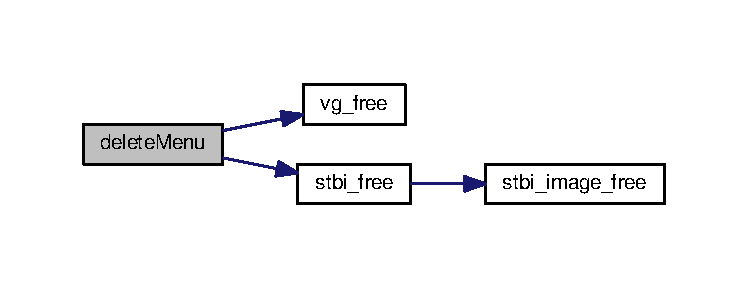
\includegraphics[width=350pt]{group__Menu_gaf155dd05949566ff9a0f29d8759bcd54_cgraph}
\end{center}
\end{figure}


\index{Menu@{Menu}!draw\+Menu@{draw\+Menu}}
\index{draw\+Menu@{draw\+Menu}!Menu@{Menu}}
\subsubsection[{\texorpdfstring{draw\+Menu(\+Menu $\ast$state)}{drawMenu(Menu *state)}}]{\setlength{\rightskip}{0pt plus 5cm}void draw\+Menu (
\begin{DoxyParamCaption}
\item[{{\bf Menu} $\ast$}]{state}
\end{DoxyParamCaption}
)}\hypertarget{group__Menu_gaf953dd83cbfca767233cb1c5f78eb266}{}\label{group__Menu_gaf953dd83cbfca767233cb1c5f78eb266}


draws \hyperlink{structMenu}{Menu} 


\begin{DoxyParams}{Parameters}
{\em state} & pointer to the \hyperlink{structMenu}{Menu} that is to be drawn \\
\hline
\end{DoxyParams}


Here is the call graph for this function\+:
\nopagebreak
\begin{figure}[H]
\begin{center}
\leavevmode
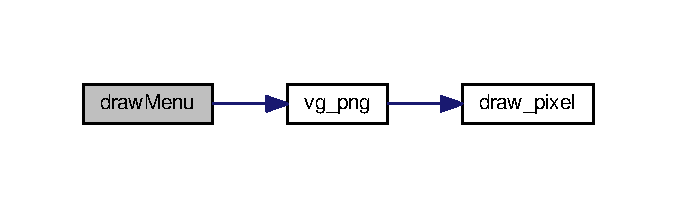
\includegraphics[width=325pt]{group__Menu_gaf953dd83cbfca767233cb1c5f78eb266_cgraph}
\end{center}
\end{figure}


\index{Menu@{Menu}!new\+Menu@{new\+Menu}}
\index{new\+Menu@{new\+Menu}!Menu@{Menu}}
\subsubsection[{\texorpdfstring{new\+Menu()}{newMenu()}}]{\setlength{\rightskip}{0pt plus 5cm}{\bf Menu}$\ast$ new\+Menu (
\begin{DoxyParamCaption}
{}
\end{DoxyParamCaption}
)}\hypertarget{group__Menu_gab4c4331657aad73fe461b1946d6a80e6}{}\label{group__Menu_gab4c4331657aad73fe461b1946d6a80e6}


creates a new \hyperlink{structMenu}{Menu} instance 

Loads Bitmaps Initializes other member of \hyperlink{structMenu}{Menu} struct

\begin{DoxyReturn}{Returns}
pointer to the \hyperlink{structMenu}{Menu} created 
\end{DoxyReturn}


Here is the call graph for this function\+:
\nopagebreak
\begin{figure}[H]
\begin{center}
\leavevmode
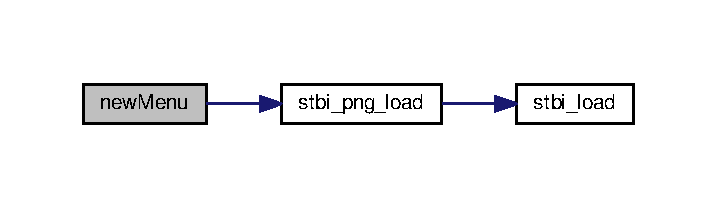
\includegraphics[width=344pt]{group__Menu_gab4c4331657aad73fe461b1946d6a80e6_cgraph}
\end{center}
\end{figure}


\index{Menu@{Menu}!update\+Menu@{update\+Menu}}
\index{update\+Menu@{update\+Menu}!Menu@{Menu}}
\subsubsection[{\texorpdfstring{update\+Menu(\+Menu $\ast$state, unsigned long scan\+\_\+code)}{updateMenu(Menu *state, unsigned long scan_code)}}]{\setlength{\rightskip}{0pt plus 5cm}void update\+Menu (
\begin{DoxyParamCaption}
\item[{{\bf Menu} $\ast$}]{state, }
\item[{unsigned long}]{scan\+\_\+code}
\end{DoxyParamCaption}
)}\hypertarget{group__Menu_gab3392fb7e40877fd1ea754606fc9f8a1}{}\label{group__Menu_gab3392fb7e40877fd1ea754606fc9f8a1}


updates the \hyperlink{structMenu}{Menu} 

Checks if the player has chosen any \hyperlink{structMenu}{Menu} option or pressed E\+SC key If yes, changes the \hyperlink{structMenu}{Menu} action according to the palyer\textquotesingle{}s choice and updates member done (=1)


\begin{DoxyParams}{Parameters}
{\em state} & pointer to the \hyperlink{structMenu}{Menu} that is to be updated\\
\hline
{\em scan\+\_\+code} & scan code from the last keyboard interrupt \\
\hline
\end{DoxyParams}


Here is the call graph for this function\+:
\nopagebreak
\begin{figure}[H]
\begin{center}
\leavevmode
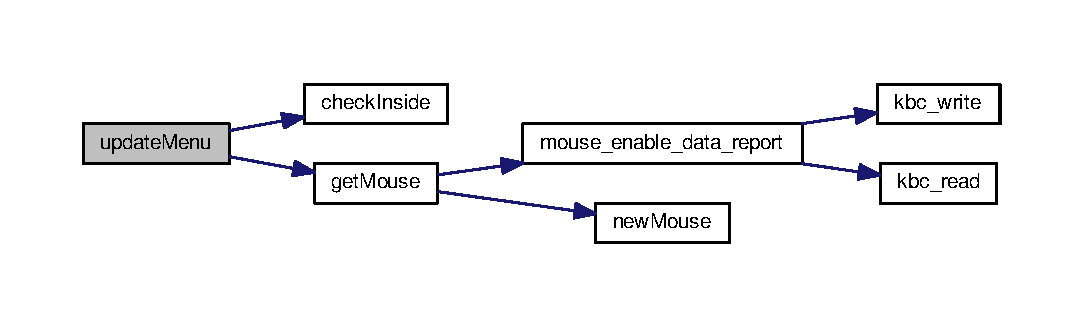
\includegraphics[width=350pt]{group__Menu_gab3392fb7e40877fd1ea754606fc9f8a1_cgraph}
\end{center}
\end{figure}



\hypertarget{group__Mouse}{}\section{Mouse}
\label{group__Mouse}\index{Mouse@{Mouse}}
\subsection*{Classes}
\begin{DoxyCompactItemize}
\item 
struct \hyperlink{structMouse}{Mouse}
\end{DoxyCompactItemize}
\subsection*{Functions}
\begin{DoxyCompactItemize}
\item 
\hyperlink{structMouse}{Mouse} $\ast$ \hyperlink{group__Mouse_gabd64fd476265e0fb0463cc3d82823701}{new\+Mouse} ()
\begin{DoxyCompactList}\small\item\em new mouse instantiation \end{DoxyCompactList}\item 
\hyperlink{structMouse}{Mouse} $\ast$ \hyperlink{group__Mouse_ga8d3f3987b96a716cc9c3aa8e484ff1d7}{get\+Mouse} ()
\begin{DoxyCompactList}\small\item\em gets the mouse object \end{DoxyCompactList}\item 
void \hyperlink{group__Mouse_ga6498182307b6c3f4a9c9c03a9d5116dc}{update\+Mouse} ()
\item 
void \hyperlink{group__Mouse_ga6a0f0fbd9fee2962ff384838bbf9fade}{draw\+Mouse} (unsigned char $\ast$cursor, int width, int height)
\begin{DoxyCompactList}\small\item\em new mouse instantiation \end{DoxyCompactList}\item 
void \hyperlink{group__Mouse_ga54e27b79923964c8882407116930fc70}{delete\+Mouse} ()
\item 
void \hyperlink{group__Mouse_ga44baaa1c128be31e1baba247c3b4b6db}{packet\+\_\+handler} ()
\item 
int \hyperlink{group__Mouse_ga5075265654e56158f16cdbb0f0e4e94b}{check\+Inside} (unsigned xi, unsigned xf, unsigned yi, unsigned yf)
\begin{DoxyCompactList}\small\item\em check if the mouse is inside the window \end{DoxyCompactList}\item 
int \hyperlink{group__Mouse_ga51e6ee02a5c0a7e618abde7250cd0841}{mouse\+\_\+subscribe\+\_\+int} (void)
\begin{DoxyCompactList}\small\item\em Subscribes and enables K\+BC interrupts. \end{DoxyCompactList}\item 
int \hyperlink{group__Mouse_ga685ad2706aca36d9869a30a19b9f446a}{mouse\+\_\+unsubscribe\+\_\+int} ()
\begin{DoxyCompactList}\small\item\em Unsubscribes K\+BC interrupts. \end{DoxyCompactList}\item 
int \hyperlink{group__Mouse_ga108813d01ba189cc8bb0dca728c932a8}{mouse\+\_\+enable\+\_\+data\+\_\+report} ()
\begin{DoxyCompactList}\small\item\em Enable mouse data report in stream mode. \end{DoxyCompactList}\item 
int \hyperlink{group__Mouse_gac13ad81d843b4d50815de4b20a28db53}{mouse\+\_\+disable\+\_\+data\+\_\+report} ()
\begin{DoxyCompactList}\small\item\em Disable mouse data report in stream mode. \end{DoxyCompactList}\item 
int \hyperlink{group__Mouse_ga16a521d1919cbd8f434d8b5d535a639b}{mouse\+\_\+set\+\_\+stream\+\_\+mode} ()
\begin{DoxyCompactList}\small\item\em Puts mouse working in stream mode. \end{DoxyCompactList}\item 
int \hyperlink{group__Mouse_ga1e54e352956b51fbf324d36d24befcbb}{mouse\+\_\+get\+\_\+packet} ()
\begin{DoxyCompactList}\small\item\em Gets the mouse packets and prints them on the screen. \end{DoxyCompactList}\end{DoxyCompactItemize}
\subsection*{Variables}
\begin{DoxyCompactItemize}
\item 
int \hyperlink{group__Mouse_ga136eea114b70f46392b89cc3779d4291}{Mouse\+::x}
\item 
int \hyperlink{group__Mouse_ga4a29b1c18faaa2fbe39ff985ba9d6737}{Mouse\+::y}
\item 
int \hyperlink{group__Mouse_ga1fc496df2223cb17437b296acbe02e50}{Mouse\+::packet\+\_\+idx}
\item 
int \hyperlink{group__Mouse_ga64798c8dfb1b60b4ce76bc9859719077}{Mouse\+::complete\+\_\+packet}
\item 
unsigned long \hyperlink{group__Mouse_ga8bfb0c35eb14423f5086a355d52dc733}{Mouse\+::packet} \mbox{[}3\mbox{]}
\item 
int \hyperlink{group__Mouse_ga401d046e1cad0fad3908120ab85b9396}{Mouse\+::left\+Button\+Down}
\item 
int \hyperlink{group__Mouse_ga9a74cd5fb66c4936d44a72962df7830c}{Mouse\+::left\+Button\+Released}
\item 
int \hyperlink{group__Mouse_gad3b4a3a6fd6d53630bdf7aa81d74f744}{Mouse\+::draw}
\end{DoxyCompactItemize}


\subsection{Detailed Description}
Functions for using the i8042 K\+BC I\+N\+T\+E\+R\+F\+A\+C\+I\+NG W\+I\+TH T\+HE M\+O\+U\+SE 

\subsection{Function Documentation}
\index{Mouse@{Mouse}!check\+Inside@{check\+Inside}}
\index{check\+Inside@{check\+Inside}!Mouse@{Mouse}}
\subsubsection[{\texorpdfstring{check\+Inside(unsigned xi, unsigned xf, unsigned yi, unsigned yf)}{checkInside(unsigned xi, unsigned xf, unsigned yi, unsigned yf)}}]{\setlength{\rightskip}{0pt plus 5cm}int check\+Inside (
\begin{DoxyParamCaption}
\item[{unsigned}]{xi, }
\item[{unsigned}]{xf, }
\item[{unsigned}]{yi, }
\item[{unsigned}]{yf}
\end{DoxyParamCaption}
)}\hypertarget{group__Mouse_ga5075265654e56158f16cdbb0f0e4e94b}{}\label{group__Mouse_ga5075265654e56158f16cdbb0f0e4e94b}


check if the mouse is inside the window 


\begin{DoxyParams}{Parameters}
{\em xi} & initial X coord\\
\hline
{\em xf} & final X coord\\
\hline
{\em yi} & initial Y coord\\
\hline
{\em yf} & final Y coord\\
\hline
\end{DoxyParams}
\begin{DoxyReturn}{Returns}
Return 0 upon success and non-\/zero otherwise 
\end{DoxyReturn}
\index{Mouse@{Mouse}!delete\+Mouse@{delete\+Mouse}}
\index{delete\+Mouse@{delete\+Mouse}!Mouse@{Mouse}}
\subsubsection[{\texorpdfstring{delete\+Mouse()}{deleteMouse()}}]{\setlength{\rightskip}{0pt plus 5cm}void delete\+Mouse (
\begin{DoxyParamCaption}
{}
\end{DoxyParamCaption}
)}\hypertarget{group__Mouse_ga54e27b79923964c8882407116930fc70}{}\label{group__Mouse_ga54e27b79923964c8882407116930fc70}


Here is the call graph for this function\+:
\nopagebreak
\begin{figure}[H]
\begin{center}
\leavevmode
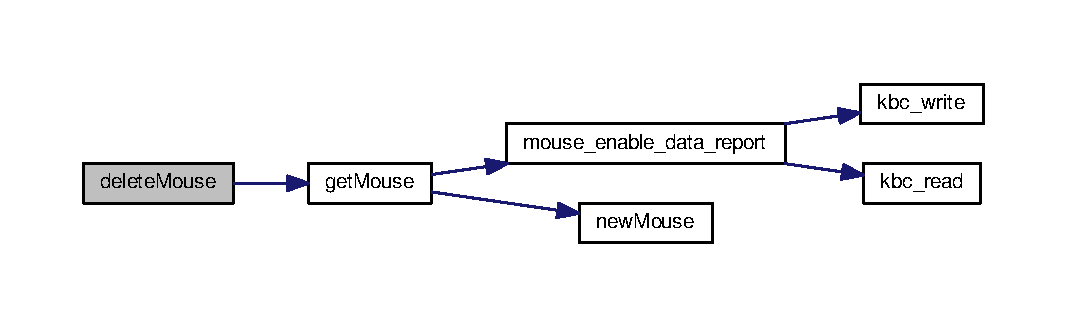
\includegraphics[width=350pt]{group__Mouse_ga54e27b79923964c8882407116930fc70_cgraph}
\end{center}
\end{figure}


\index{Mouse@{Mouse}!draw\+Mouse@{draw\+Mouse}}
\index{draw\+Mouse@{draw\+Mouse}!Mouse@{Mouse}}
\subsubsection[{\texorpdfstring{draw\+Mouse(unsigned char $\ast$cursor, int width, int height)}{drawMouse(unsigned char *cursor, int width, int height)}}]{\setlength{\rightskip}{0pt plus 5cm}void draw\+Mouse (
\begin{DoxyParamCaption}
\item[{unsigned char $\ast$}]{cursor, }
\item[{int}]{width, }
\item[{int}]{height}
\end{DoxyParamCaption}
)}\hypertarget{group__Mouse_ga6a0f0fbd9fee2962ff384838bbf9fade}{}\label{group__Mouse_ga6a0f0fbd9fee2962ff384838bbf9fade}


new mouse instantiation 


\begin{DoxyParams}{Parameters}
{\em cursor} & the mouse cursor image\\
\hline
{\em width} & the mouse cursor image width\\
\hline
{\em width} & the mouse cursor image height \\
\hline
\end{DoxyParams}


Here is the call graph for this function\+:
\nopagebreak
\begin{figure}[H]
\begin{center}
\leavevmode
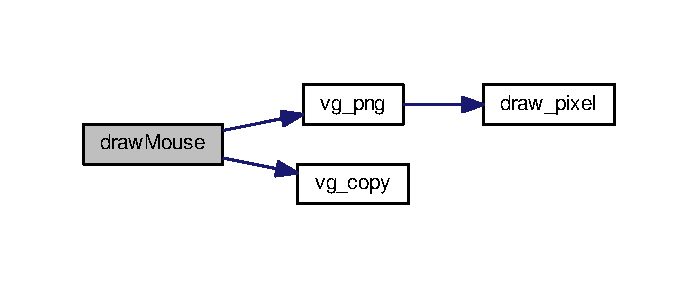
\includegraphics[width=335pt]{group__Mouse_ga6a0f0fbd9fee2962ff384838bbf9fade_cgraph}
\end{center}
\end{figure}


\index{Mouse@{Mouse}!get\+Mouse@{get\+Mouse}}
\index{get\+Mouse@{get\+Mouse}!Mouse@{Mouse}}
\subsubsection[{\texorpdfstring{get\+Mouse()}{getMouse()}}]{\setlength{\rightskip}{0pt plus 5cm}{\bf Mouse}$\ast$ get\+Mouse (
\begin{DoxyParamCaption}
{}
\end{DoxyParamCaption}
)}\hypertarget{group__Mouse_ga8d3f3987b96a716cc9c3aa8e484ff1d7}{}\label{group__Mouse_ga8d3f3987b96a716cc9c3aa8e484ff1d7}


gets the mouse object 

\begin{DoxyReturn}{Returns}
mouse object 
\end{DoxyReturn}


Here is the call graph for this function\+:
\nopagebreak
\begin{figure}[H]
\begin{center}
\leavevmode
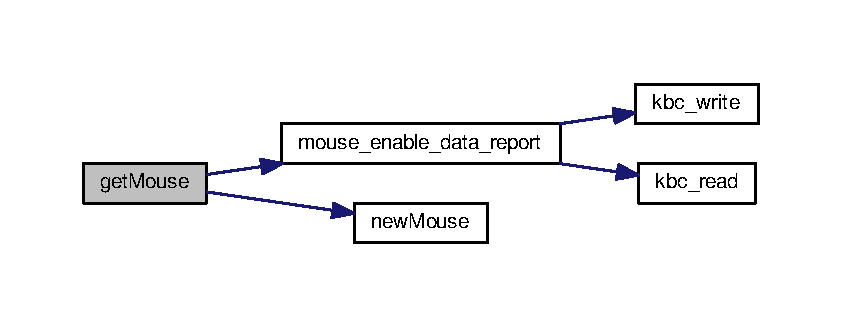
\includegraphics[width=350pt]{group__Mouse_ga8d3f3987b96a716cc9c3aa8e484ff1d7_cgraph}
\end{center}
\end{figure}


\index{Mouse@{Mouse}!mouse\+\_\+disable\+\_\+data\+\_\+report@{mouse\+\_\+disable\+\_\+data\+\_\+report}}
\index{mouse\+\_\+disable\+\_\+data\+\_\+report@{mouse\+\_\+disable\+\_\+data\+\_\+report}!Mouse@{Mouse}}
\subsubsection[{\texorpdfstring{mouse\+\_\+disable\+\_\+data\+\_\+report()}{mouse_disable_data_report()}}]{\setlength{\rightskip}{0pt plus 5cm}int mouse\+\_\+disable\+\_\+data\+\_\+report (
\begin{DoxyParamCaption}
{}
\end{DoxyParamCaption}
)}\hypertarget{group__Mouse_gac13ad81d843b4d50815de4b20a28db53}{}\label{group__Mouse_gac13ad81d843b4d50815de4b20a28db53}


Disable mouse data report in stream mode. 

\begin{DoxyReturn}{Returns}
Returns A\+CK, N\+A\+CK or E\+R\+R\+OR 
\end{DoxyReturn}


Here is the call graph for this function\+:
\nopagebreak
\begin{figure}[H]
\begin{center}
\leavevmode
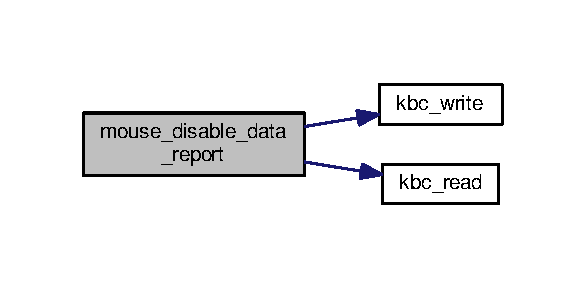
\includegraphics[width=281pt]{group__Mouse_gac13ad81d843b4d50815de4b20a28db53_cgraph}
\end{center}
\end{figure}


\index{Mouse@{Mouse}!mouse\+\_\+enable\+\_\+data\+\_\+report@{mouse\+\_\+enable\+\_\+data\+\_\+report}}
\index{mouse\+\_\+enable\+\_\+data\+\_\+report@{mouse\+\_\+enable\+\_\+data\+\_\+report}!Mouse@{Mouse}}
\subsubsection[{\texorpdfstring{mouse\+\_\+enable\+\_\+data\+\_\+report()}{mouse_enable_data_report()}}]{\setlength{\rightskip}{0pt plus 5cm}int mouse\+\_\+enable\+\_\+data\+\_\+report (
\begin{DoxyParamCaption}
{}
\end{DoxyParamCaption}
)}\hypertarget{group__Mouse_ga108813d01ba189cc8bb0dca728c932a8}{}\label{group__Mouse_ga108813d01ba189cc8bb0dca728c932a8}


Enable mouse data report in stream mode. 

\begin{DoxyReturn}{Returns}
Returns A\+CK, N\+A\+CK or E\+R\+R\+OR 
\end{DoxyReturn}


Here is the call graph for this function\+:
\nopagebreak
\begin{figure}[H]
\begin{center}
\leavevmode
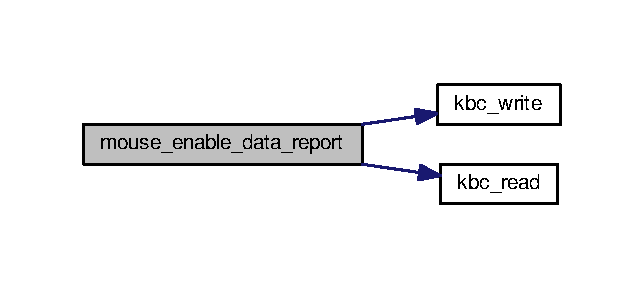
\includegraphics[width=309pt]{group__Mouse_ga108813d01ba189cc8bb0dca728c932a8_cgraph}
\end{center}
\end{figure}


\index{Mouse@{Mouse}!mouse\+\_\+get\+\_\+packet@{mouse\+\_\+get\+\_\+packet}}
\index{mouse\+\_\+get\+\_\+packet@{mouse\+\_\+get\+\_\+packet}!Mouse@{Mouse}}
\subsubsection[{\texorpdfstring{mouse\+\_\+get\+\_\+packet()}{mouse_get_packet()}}]{\setlength{\rightskip}{0pt plus 5cm}int mouse\+\_\+get\+\_\+packet (
\begin{DoxyParamCaption}
{}
\end{DoxyParamCaption}
)}\hypertarget{group__Mouse_ga1e54e352956b51fbf324d36d24befcbb}{}\label{group__Mouse_ga1e54e352956b51fbf324d36d24befcbb}


Gets the mouse packets and prints them on the screen. 

\begin{DoxyReturn}{Returns}
1 in case of success, 0 otherwise 
\end{DoxyReturn}


Here is the call graph for this function\+:
\nopagebreak
\begin{figure}[H]
\begin{center}
\leavevmode
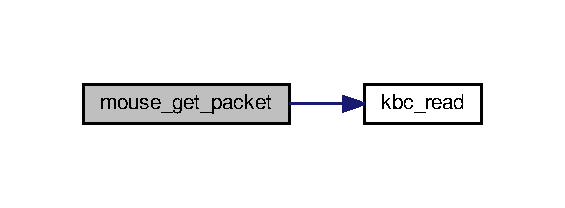
\includegraphics[width=271pt]{group__Mouse_ga1e54e352956b51fbf324d36d24befcbb_cgraph}
\end{center}
\end{figure}


\index{Mouse@{Mouse}!mouse\+\_\+set\+\_\+stream\+\_\+mode@{mouse\+\_\+set\+\_\+stream\+\_\+mode}}
\index{mouse\+\_\+set\+\_\+stream\+\_\+mode@{mouse\+\_\+set\+\_\+stream\+\_\+mode}!Mouse@{Mouse}}
\subsubsection[{\texorpdfstring{mouse\+\_\+set\+\_\+stream\+\_\+mode()}{mouse_set_stream_mode()}}]{\setlength{\rightskip}{0pt plus 5cm}int mouse\+\_\+set\+\_\+stream\+\_\+mode (
\begin{DoxyParamCaption}
{}
\end{DoxyParamCaption}
)}\hypertarget{group__Mouse_ga16a521d1919cbd8f434d8b5d535a639b}{}\label{group__Mouse_ga16a521d1919cbd8f434d8b5d535a639b}


Puts mouse working in stream mode. 

\begin{DoxyReturn}{Returns}
Returns A\+CK, N\+A\+CK or E\+R\+R\+OR 
\end{DoxyReturn}


Here is the call graph for this function\+:
\nopagebreak
\begin{figure}[H]
\begin{center}
\leavevmode
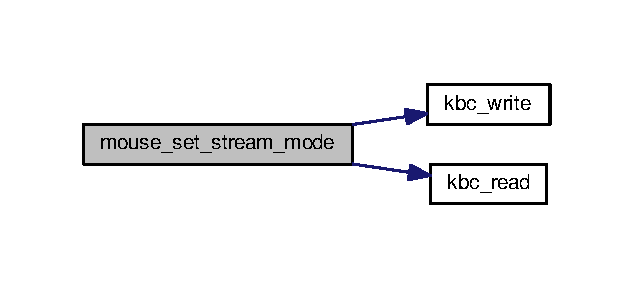
\includegraphics[width=304pt]{group__Mouse_ga16a521d1919cbd8f434d8b5d535a639b_cgraph}
\end{center}
\end{figure}


\index{Mouse@{Mouse}!mouse\+\_\+subscribe\+\_\+int@{mouse\+\_\+subscribe\+\_\+int}}
\index{mouse\+\_\+subscribe\+\_\+int@{mouse\+\_\+subscribe\+\_\+int}!Mouse@{Mouse}}
\subsubsection[{\texorpdfstring{mouse\+\_\+subscribe\+\_\+int(void)}{mouse_subscribe_int(void)}}]{\setlength{\rightskip}{0pt plus 5cm}int mouse\+\_\+subscribe\+\_\+int (
\begin{DoxyParamCaption}
\item[{void}]{}
\end{DoxyParamCaption}
)}\hypertarget{group__Mouse_ga51e6ee02a5c0a7e618abde7250cd0841}{}\label{group__Mouse_ga51e6ee02a5c0a7e618abde7250cd0841}


Subscribes and enables K\+BC interrupts. 

\begin{DoxyReturn}{Returns}
Returns bit order in interrupt mask; negative value on failure 
\end{DoxyReturn}
\index{Mouse@{Mouse}!mouse\+\_\+unsubscribe\+\_\+int@{mouse\+\_\+unsubscribe\+\_\+int}}
\index{mouse\+\_\+unsubscribe\+\_\+int@{mouse\+\_\+unsubscribe\+\_\+int}!Mouse@{Mouse}}
\subsubsection[{\texorpdfstring{mouse\+\_\+unsubscribe\+\_\+int()}{mouse_unsubscribe_int()}}]{\setlength{\rightskip}{0pt plus 5cm}int mouse\+\_\+unsubscribe\+\_\+int (
\begin{DoxyParamCaption}
{}
\end{DoxyParamCaption}
)}\hypertarget{group__Mouse_ga685ad2706aca36d9869a30a19b9f446a}{}\label{group__Mouse_ga685ad2706aca36d9869a30a19b9f446a}


Unsubscribes K\+BC interrupts. 

\begin{DoxyReturn}{Returns}
Return 0 upon success and non-\/zero otherwise 
\end{DoxyReturn}
\index{Mouse@{Mouse}!new\+Mouse@{new\+Mouse}}
\index{new\+Mouse@{new\+Mouse}!Mouse@{Mouse}}
\subsubsection[{\texorpdfstring{new\+Mouse()}{newMouse()}}]{\setlength{\rightskip}{0pt plus 5cm}{\bf Mouse}$\ast$ new\+Mouse (
\begin{DoxyParamCaption}
{}
\end{DoxyParamCaption}
)}\hypertarget{group__Mouse_gabd64fd476265e0fb0463cc3d82823701}{}\label{group__Mouse_gabd64fd476265e0fb0463cc3d82823701}


new mouse instantiation 

\begin{DoxyReturn}{Returns}
mouse object 
\end{DoxyReturn}
\index{Mouse@{Mouse}!packet\+\_\+handler@{packet\+\_\+handler}}
\index{packet\+\_\+handler@{packet\+\_\+handler}!Mouse@{Mouse}}
\subsubsection[{\texorpdfstring{packet\+\_\+handler()}{packet_handler()}}]{\setlength{\rightskip}{0pt plus 5cm}void packet\+\_\+handler (
\begin{DoxyParamCaption}
{}
\end{DoxyParamCaption}
)}\hypertarget{group__Mouse_ga44baaa1c128be31e1baba247c3b4b6db}{}\label{group__Mouse_ga44baaa1c128be31e1baba247c3b4b6db}
\index{Mouse@{Mouse}!update\+Mouse@{update\+Mouse}}
\index{update\+Mouse@{update\+Mouse}!Mouse@{Mouse}}
\subsubsection[{\texorpdfstring{update\+Mouse()}{updateMouse()}}]{\setlength{\rightskip}{0pt plus 5cm}void update\+Mouse (
\begin{DoxyParamCaption}
{}
\end{DoxyParamCaption}
)}\hypertarget{group__Mouse_ga6498182307b6c3f4a9c9c03a9d5116dc}{}\label{group__Mouse_ga6498182307b6c3f4a9c9c03a9d5116dc}


Here is the call graph for this function\+:
\nopagebreak
\begin{figure}[H]
\begin{center}
\leavevmode
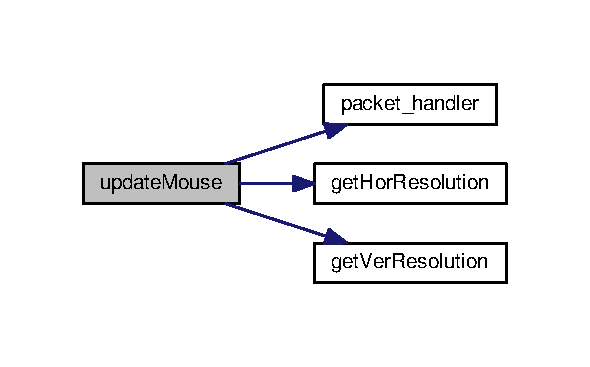
\includegraphics[width=283pt]{group__Mouse_ga6498182307b6c3f4a9c9c03a9d5116dc_cgraph}
\end{center}
\end{figure}




\subsection{Variable Documentation}
\index{Mouse@{Mouse}!complete\+\_\+packet@{complete\+\_\+packet}}
\index{complete\+\_\+packet@{complete\+\_\+packet}!Mouse@{Mouse}}
\subsubsection[{\texorpdfstring{complete\+\_\+packet}{complete_packet}}]{\setlength{\rightskip}{0pt plus 5cm}int Mouse\+::complete\+\_\+packet}\hypertarget{group__Mouse_ga64798c8dfb1b60b4ce76bc9859719077}{}\label{group__Mouse_ga64798c8dfb1b60b4ce76bc9859719077}
1 if packet is ready to be read, 0 otherwise \index{Mouse@{Mouse}!draw@{draw}}
\index{draw@{draw}!Mouse@{Mouse}}
\subsubsection[{\texorpdfstring{draw}{draw}}]{\setlength{\rightskip}{0pt plus 5cm}int Mouse\+::draw}\hypertarget{group__Mouse_gad3b4a3a6fd6d53630bdf7aa81d74f744}{}\label{group__Mouse_gad3b4a3a6fd6d53630bdf7aa81d74f744}
1 if mouse must be displayed on the screen, 0 otherwise \index{Mouse@{Mouse}!left\+Button\+Down@{left\+Button\+Down}}
\index{left\+Button\+Down@{left\+Button\+Down}!Mouse@{Mouse}}
\subsubsection[{\texorpdfstring{left\+Button\+Down}{leftButtonDown}}]{\setlength{\rightskip}{0pt plus 5cm}int Mouse\+::left\+Button\+Down}\hypertarget{group__Mouse_ga401d046e1cad0fad3908120ab85b9396}{}\label{group__Mouse_ga401d046e1cad0fad3908120ab85b9396}
1 if mouse\textquotesingle{}s left button is being pressed, 0 otherwise \index{Mouse@{Mouse}!left\+Button\+Released@{left\+Button\+Released}}
\index{left\+Button\+Released@{left\+Button\+Released}!Mouse@{Mouse}}
\subsubsection[{\texorpdfstring{left\+Button\+Released}{leftButtonReleased}}]{\setlength{\rightskip}{0pt plus 5cm}int Mouse\+::left\+Button\+Released}\hypertarget{group__Mouse_ga9a74cd5fb66c4936d44a72962df7830c}{}\label{group__Mouse_ga9a74cd5fb66c4936d44a72962df7830c}
1 if mouse\textquotesingle{}s left button has just been released, 0 otherwise \index{Mouse@{Mouse}!packet@{packet}}
\index{packet@{packet}!Mouse@{Mouse}}
\subsubsection[{\texorpdfstring{packet}{packet}}]{\setlength{\rightskip}{0pt plus 5cm}unsigned long Mouse\+::packet\mbox{[}3\mbox{]}}\hypertarget{group__Mouse_ga8bfb0c35eb14423f5086a355d52dc733}{}\label{group__Mouse_ga8bfb0c35eb14423f5086a355d52dc733}
array containing the 3 mouse packets \index{Mouse@{Mouse}!packet\+\_\+idx@{packet\+\_\+idx}}
\index{packet\+\_\+idx@{packet\+\_\+idx}!Mouse@{Mouse}}
\subsubsection[{\texorpdfstring{packet\+\_\+idx}{packet_idx}}]{\setlength{\rightskip}{0pt plus 5cm}int Mouse\+::packet\+\_\+idx}\hypertarget{group__Mouse_ga1fc496df2223cb17437b296acbe02e50}{}\label{group__Mouse_ga1fc496df2223cb17437b296acbe02e50}
index of the packet being currently read \index{Mouse@{Mouse}!x@{x}}
\index{x@{x}!Mouse@{Mouse}}
\subsubsection[{\texorpdfstring{x}{x}}]{\setlength{\rightskip}{0pt plus 5cm}int Mouse\+::x}\hypertarget{group__Mouse_ga136eea114b70f46392b89cc3779d4291}{}\label{group__Mouse_ga136eea114b70f46392b89cc3779d4291}
mouse x coordinate \index{Mouse@{Mouse}!y@{y}}
\index{y@{y}!Mouse@{Mouse}}
\subsubsection[{\texorpdfstring{y}{y}}]{\setlength{\rightskip}{0pt plus 5cm}int Mouse\+::y}\hypertarget{group__Mouse_ga4a29b1c18faaa2fbe39ff985ba9d6737}{}\label{group__Mouse_ga4a29b1c18faaa2fbe39ff985ba9d6737}
mouse y coordinate 
\hypertarget{group__timer}{}\section{timer}
\label{group__timer}\index{timer@{timer}}
\subsection*{Functions}
\begin{DoxyCompactItemize}
\item 
int \hyperlink{group__timer_ga4c5d9f47323eda494cfd826f6d62eec9}{timer\+\_\+subscribe\+\_\+int} (void)
\begin{DoxyCompactList}\small\item\em Subscribes and enables Timer 0 interrupts. \end{DoxyCompactList}\item 
int \hyperlink{group__timer_gab9eea51549744bca5c5c923b388bb4ee}{timer\+\_\+unsubscribe\+\_\+int} ()
\begin{DoxyCompactList}\small\item\em Unsubscribes Timer 0 interrupts. \end{DoxyCompactList}\item 
void \hyperlink{group__timer_ga10fc9c867b15c7da6649311c9987cd17}{timer\+\_\+int\+\_\+handler} ()
\begin{DoxyCompactList}\small\item\em Timer 0 interrupt handler. \end{DoxyCompactList}\end{DoxyCompactItemize}
\subsection*{Variables}
\begin{DoxyCompactItemize}
\item 
int \hyperlink{group__timer_ga617a47c70795bcff659815ad0efd2266}{counter}
\end{DoxyCompactItemize}


\subsection{Detailed Description}
Functions for using the i8254 timers 

\subsection{Function Documentation}
\index{timer@{timer}!timer\+\_\+int\+\_\+handler@{timer\+\_\+int\+\_\+handler}}
\index{timer\+\_\+int\+\_\+handler@{timer\+\_\+int\+\_\+handler}!timer@{timer}}
\subsubsection[{\texorpdfstring{timer\+\_\+int\+\_\+handler()}{timer_int_handler()}}]{\setlength{\rightskip}{0pt plus 5cm}void timer\+\_\+int\+\_\+handler (
\begin{DoxyParamCaption}
{}
\end{DoxyParamCaption}
)}\hypertarget{group__timer_ga10fc9c867b15c7da6649311c9987cd17}{}\label{group__timer_ga10fc9c867b15c7da6649311c9987cd17}


Timer 0 interrupt handler. 

Increments counter \index{timer@{timer}!timer\+\_\+subscribe\+\_\+int@{timer\+\_\+subscribe\+\_\+int}}
\index{timer\+\_\+subscribe\+\_\+int@{timer\+\_\+subscribe\+\_\+int}!timer@{timer}}
\subsubsection[{\texorpdfstring{timer\+\_\+subscribe\+\_\+int(void)}{timer_subscribe_int(void)}}]{\setlength{\rightskip}{0pt plus 5cm}int timer\+\_\+subscribe\+\_\+int (
\begin{DoxyParamCaption}
\item[{void}]{}
\end{DoxyParamCaption}
)}\hypertarget{group__timer_ga4c5d9f47323eda494cfd826f6d62eec9}{}\label{group__timer_ga4c5d9f47323eda494cfd826f6d62eec9}


Subscribes and enables Timer 0 interrupts. 

\begin{DoxyReturn}{Returns}
Returns bit order in interrupt mask; negative value on failure 
\end{DoxyReturn}
\index{timer@{timer}!timer\+\_\+unsubscribe\+\_\+int@{timer\+\_\+unsubscribe\+\_\+int}}
\index{timer\+\_\+unsubscribe\+\_\+int@{timer\+\_\+unsubscribe\+\_\+int}!timer@{timer}}
\subsubsection[{\texorpdfstring{timer\+\_\+unsubscribe\+\_\+int()}{timer_unsubscribe_int()}}]{\setlength{\rightskip}{0pt plus 5cm}int timer\+\_\+unsubscribe\+\_\+int (
\begin{DoxyParamCaption}
{}
\end{DoxyParamCaption}
)}\hypertarget{group__timer_gab9eea51549744bca5c5c923b388bb4ee}{}\label{group__timer_gab9eea51549744bca5c5c923b388bb4ee}


Unsubscribes Timer 0 interrupts. 

\begin{DoxyReturn}{Returns}
Return 0 upon success and non-\/zero otherwise 
\end{DoxyReturn}


\subsection{Variable Documentation}
\index{timer@{timer}!counter@{counter}}
\index{counter@{counter}!timer@{timer}}
\subsubsection[{\texorpdfstring{counter}{counter}}]{\setlength{\rightskip}{0pt plus 5cm}int counter}\hypertarget{group__timer_ga617a47c70795bcff659815ad0efd2266}{}\label{group__timer_ga617a47c70795bcff659815ad0efd2266}

\hypertarget{group__vbe}{}\section{vbe}
\label{group__vbe}\index{vbe@{vbe}}
\subsection*{Classes}
\begin{DoxyCompactItemize}
\item 
struct \hyperlink{struct____attribute____}{\+\_\+\+\_\+attribute\+\_\+\+\_\+}
\end{DoxyCompactItemize}
\subsection*{Functions}
\begin{DoxyCompactItemize}
\item 
int \hyperlink{group__vbe_ga4ef3234e41f2050bc094a22049b69e45}{vbe\+\_\+get\+\_\+mode\+\_\+info} (unsigned short mode, vbe\+\_\+mode\+\_\+info\+\_\+t $\ast$vmi\+\_\+p)
\begin{DoxyCompactList}\small\item\em Returns information on the input V\+BE mode, including screen dimensions, color depth and V\+R\+AM physical address. \end{DoxyCompactList}\end{DoxyCompactItemize}


\subsection{Detailed Description}
Functions related to the V\+BE standard 

\subsection{Function Documentation}
\index{vbe@{vbe}!vbe\+\_\+get\+\_\+mode\+\_\+info@{vbe\+\_\+get\+\_\+mode\+\_\+info}}
\index{vbe\+\_\+get\+\_\+mode\+\_\+info@{vbe\+\_\+get\+\_\+mode\+\_\+info}!vbe@{vbe}}
\subsubsection[{\texorpdfstring{vbe\+\_\+get\+\_\+mode\+\_\+info(unsigned short mode, vbe\+\_\+mode\+\_\+info\+\_\+t $\ast$vmi\+\_\+p)}{vbe_get_mode_info(unsigned short mode, vbe_mode_info_t *vmi_p)}}]{\setlength{\rightskip}{0pt plus 5cm}int vbe\+\_\+get\+\_\+mode\+\_\+info (
\begin{DoxyParamCaption}
\item[{unsigned short}]{mode, }
\item[{vbe\+\_\+mode\+\_\+info\+\_\+t $\ast$}]{vmi\+\_\+p}
\end{DoxyParamCaption}
)}\hypertarget{group__vbe_ga4ef3234e41f2050bc094a22049b69e45}{}\label{group__vbe_ga4ef3234e41f2050bc094a22049b69e45}


Returns information on the input V\+BE mode, including screen dimensions, color depth and V\+R\+AM physical address. 

Initializes unpacked vbe\+\_\+mode\+\_\+\+\_\+info\+\_\+t structure passed as an address with the information of the input mode, by calling V\+BE function 0x01 Return V\+BE Mode Information and unpacking the Mode\+Info\+Block struct returned by that function.


\begin{DoxyParams}{Parameters}
{\em mode} & mode whose information should be returned \\
\hline
{\em vmi\+\_\+p} & address of vbe\+\_\+mode\+\_\+info\+\_\+t structure to be initialized \\
\hline
\end{DoxyParams}
\begin{DoxyReturn}{Returns}
0 on success, non-\/zero otherwise 
\end{DoxyReturn}


Here is the call graph for this function\+:
\nopagebreak
\begin{figure}[H]
\begin{center}
\leavevmode
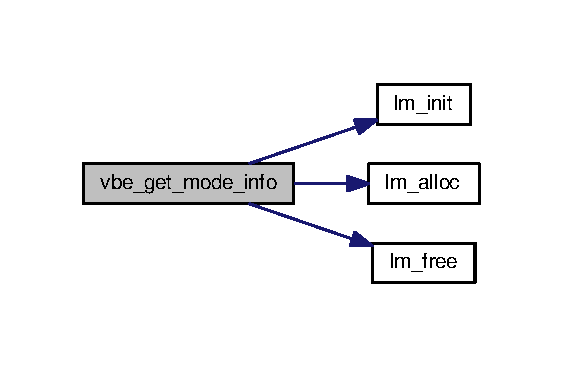
\includegraphics[width=270pt]{group__vbe_ga4ef3234e41f2050bc094a22049b69e45_cgraph}
\end{center}
\end{figure}



\hypertarget{group__video__gr}{}\section{video\+\_\+gr}
\label{group__video__gr}\index{video\+\_\+gr@{video\+\_\+gr}}
\subsection*{Functions}
\begin{DoxyCompactItemize}
\item 
void $\ast$ \hyperlink{group__video__gr_gacef21667c79365d57a084bed994c2189}{vg\+\_\+init} (unsigned short mode)
\begin{DoxyCompactList}\small\item\em Initializes the video module in graphics mode. \end{DoxyCompactList}\item 
int \hyperlink{group__video__gr_ga42f593e6656f1a978315aff02b1bcebf}{vg\+\_\+exit} (void)
\begin{DoxyCompactList}\small\item\em Returns to default Minix 3 text mode (0x03\+: 25 x 80, 16 colors) \end{DoxyCompactList}\item 
int \hyperlink{group__video__gr_ga511311dbbd19f3b1f0c99111eee21b9a}{vg\+\_\+draw\+\_\+pixel} (unsigned short x, unsigned short y, unsigned long color)
\begin{DoxyCompactList}\small\item\em draws one pixel on the screen \end{DoxyCompactList}\item 
unsigned long \hyperlink{group__video__gr_ga21e5df0f0f8fe4b0fa3841550da32c62}{vg\+\_\+get\+Color} (unsigned short x, unsigned short y)
\begin{DoxyCompactList}\small\item\em gets a pixel color \end{DoxyCompactList}\item 
void \hyperlink{group__video__gr_ga58144867b7ba0851547e9a599b05107b}{vg\+\_\+draw\+\_\+bike} (unsigned short x, unsigned short y, unsigned long color)
\begin{DoxyCompactList}\small\item\em draws the bike \end{DoxyCompactList}\item 
char $\ast$ \hyperlink{group__video__gr_gaedd0b1a041eee82028cf2c5d581ee0a6}{get\+Secondary\+Buffer} ()
\begin{DoxyCompactList}\small\item\em return the secondary buffer address \end{DoxyCompactList}\item 
int \hyperlink{group__video__gr_ga1eee563c2d26857ee2e35d7e8656e841}{get\+Ver\+Resolution} ()
\begin{DoxyCompactList}\small\item\em gets vertical resolution \end{DoxyCompactList}\item 
int \hyperlink{group__video__gr_ga85f07897fcef302cfd16a33cb690a70a}{get\+Hor\+Resolution} ()
\begin{DoxyCompactList}\small\item\em gets horizontal resolution \end{DoxyCompactList}\item 
void \hyperlink{group__video__gr_gaa1defaab9e74b37f6c3e7ec3e83a95a3}{draw\+\_\+pixel} (int x, int y, int color)
\item 
void \hyperlink{group__video__gr_gab27465d29f462aeaf3e710695fc20594}{vg\+\_\+png} (unsigned char $\ast$image, int width, int height, int start\+\_\+x, int start\+\_\+y)
\item 
void \hyperlink{group__video__gr_gae73efbc5eb5fa85cab0358d0e4de8809}{vg\+\_\+clear} ()
\item 
void \hyperlink{group__video__gr_ga6a48d2eaa7f116fca3dde151edee4f98}{vg\+\_\+copy} ()
\item 
void \hyperlink{group__video__gr_ga71250a7e4fc5b89a38e76c7d68f3a5fc}{vg\+\_\+free} ()
\end{DoxyCompactItemize}


\subsection{Detailed Description}
Functions for outputing data to screen in graphics mode 

\subsection{Function Documentation}
\index{video\+\_\+gr@{video\+\_\+gr}!draw\+\_\+pixel@{draw\+\_\+pixel}}
\index{draw\+\_\+pixel@{draw\+\_\+pixel}!video\+\_\+gr@{video\+\_\+gr}}
\subsubsection[{\texorpdfstring{draw\+\_\+pixel(int x, int y, int color)}{draw_pixel(int x, int y, int color)}}]{\setlength{\rightskip}{0pt plus 5cm}void draw\+\_\+pixel (
\begin{DoxyParamCaption}
\item[{int}]{x, }
\item[{int}]{y, }
\item[{int}]{color}
\end{DoxyParamCaption}
)}\hypertarget{group__video__gr_gaa1defaab9e74b37f6c3e7ec3e83a95a3}{}\label{group__video__gr_gaa1defaab9e74b37f6c3e7ec3e83a95a3}
\index{video\+\_\+gr@{video\+\_\+gr}!get\+Hor\+Resolution@{get\+Hor\+Resolution}}
\index{get\+Hor\+Resolution@{get\+Hor\+Resolution}!video\+\_\+gr@{video\+\_\+gr}}
\subsubsection[{\texorpdfstring{get\+Hor\+Resolution()}{getHorResolution()}}]{\setlength{\rightskip}{0pt plus 5cm}int get\+Hor\+Resolution (
\begin{DoxyParamCaption}
{}
\end{DoxyParamCaption}
)}\hypertarget{group__video__gr_ga85f07897fcef302cfd16a33cb690a70a}{}\label{group__video__gr_ga85f07897fcef302cfd16a33cb690a70a}


gets horizontal resolution 

\begin{DoxyReturn}{Returns}
horizontal resolution 
\end{DoxyReturn}
\index{video\+\_\+gr@{video\+\_\+gr}!get\+Secondary\+Buffer@{get\+Secondary\+Buffer}}
\index{get\+Secondary\+Buffer@{get\+Secondary\+Buffer}!video\+\_\+gr@{video\+\_\+gr}}
\subsubsection[{\texorpdfstring{get\+Secondary\+Buffer()}{getSecondaryBuffer()}}]{\setlength{\rightskip}{0pt plus 5cm}char$\ast$ get\+Secondary\+Buffer (
\begin{DoxyParamCaption}
{}
\end{DoxyParamCaption}
)}\hypertarget{group__video__gr_gaedd0b1a041eee82028cf2c5d581ee0a6}{}\label{group__video__gr_gaedd0b1a041eee82028cf2c5d581ee0a6}


return the secondary buffer address 

\begin{DoxyReturn}{Returns}
secondary buffer address 
\end{DoxyReturn}
\index{video\+\_\+gr@{video\+\_\+gr}!get\+Ver\+Resolution@{get\+Ver\+Resolution}}
\index{get\+Ver\+Resolution@{get\+Ver\+Resolution}!video\+\_\+gr@{video\+\_\+gr}}
\subsubsection[{\texorpdfstring{get\+Ver\+Resolution()}{getVerResolution()}}]{\setlength{\rightskip}{0pt plus 5cm}int get\+Ver\+Resolution (
\begin{DoxyParamCaption}
{}
\end{DoxyParamCaption}
)}\hypertarget{group__video__gr_ga1eee563c2d26857ee2e35d7e8656e841}{}\label{group__video__gr_ga1eee563c2d26857ee2e35d7e8656e841}


gets vertical resolution 

\begin{DoxyReturn}{Returns}
vertical resolution 
\end{DoxyReturn}
\index{video\+\_\+gr@{video\+\_\+gr}!vg\+\_\+clear@{vg\+\_\+clear}}
\index{vg\+\_\+clear@{vg\+\_\+clear}!video\+\_\+gr@{video\+\_\+gr}}
\subsubsection[{\texorpdfstring{vg\+\_\+clear()}{vg_clear()}}]{\setlength{\rightskip}{0pt plus 5cm}void vg\+\_\+clear (
\begin{DoxyParamCaption}
{}
\end{DoxyParamCaption}
)}\hypertarget{group__video__gr_gae73efbc5eb5fa85cab0358d0e4de8809}{}\label{group__video__gr_gae73efbc5eb5fa85cab0358d0e4de8809}
\index{video\+\_\+gr@{video\+\_\+gr}!vg\+\_\+copy@{vg\+\_\+copy}}
\index{vg\+\_\+copy@{vg\+\_\+copy}!video\+\_\+gr@{video\+\_\+gr}}
\subsubsection[{\texorpdfstring{vg\+\_\+copy()}{vg_copy()}}]{\setlength{\rightskip}{0pt plus 5cm}void vg\+\_\+copy (
\begin{DoxyParamCaption}
{}
\end{DoxyParamCaption}
)}\hypertarget{group__video__gr_ga6a48d2eaa7f116fca3dde151edee4f98}{}\label{group__video__gr_ga6a48d2eaa7f116fca3dde151edee4f98}
\index{video\+\_\+gr@{video\+\_\+gr}!vg\+\_\+draw\+\_\+bike@{vg\+\_\+draw\+\_\+bike}}
\index{vg\+\_\+draw\+\_\+bike@{vg\+\_\+draw\+\_\+bike}!video\+\_\+gr@{video\+\_\+gr}}
\subsubsection[{\texorpdfstring{vg\+\_\+draw\+\_\+bike(unsigned short x, unsigned short y, unsigned long color)}{vg_draw_bike(unsigned short x, unsigned short y, unsigned long color)}}]{\setlength{\rightskip}{0pt plus 5cm}void vg\+\_\+draw\+\_\+bike (
\begin{DoxyParamCaption}
\item[{unsigned short}]{x, }
\item[{unsigned short}]{y, }
\item[{unsigned long}]{color}
\end{DoxyParamCaption}
)}\hypertarget{group__video__gr_ga58144867b7ba0851547e9a599b05107b}{}\label{group__video__gr_ga58144867b7ba0851547e9a599b05107b}


draws the bike 


\begin{DoxyParams}{Parameters}
{\em x} & pixel x coord\\
\hline
{\em y} & pixel y coord\\
\hline
{\em color} & pixel color\\
\hline
\end{DoxyParams}
\begin{DoxyReturn}{Returns}
0 upon success, non-\/zero upon failure 
\end{DoxyReturn}


Here is the call graph for this function\+:
\nopagebreak
\begin{figure}[H]
\begin{center}
\leavevmode
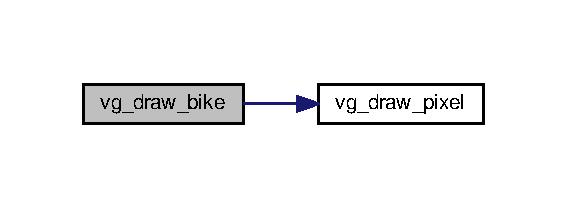
\includegraphics[width=272pt]{group__video__gr_ga58144867b7ba0851547e9a599b05107b_cgraph}
\end{center}
\end{figure}


\index{video\+\_\+gr@{video\+\_\+gr}!vg\+\_\+draw\+\_\+pixel@{vg\+\_\+draw\+\_\+pixel}}
\index{vg\+\_\+draw\+\_\+pixel@{vg\+\_\+draw\+\_\+pixel}!video\+\_\+gr@{video\+\_\+gr}}
\subsubsection[{\texorpdfstring{vg\+\_\+draw\+\_\+pixel(unsigned short x, unsigned short y, unsigned long color)}{vg_draw_pixel(unsigned short x, unsigned short y, unsigned long color)}}]{\setlength{\rightskip}{0pt plus 5cm}int vg\+\_\+draw\+\_\+pixel (
\begin{DoxyParamCaption}
\item[{unsigned short}]{x, }
\item[{unsigned short}]{y, }
\item[{unsigned long}]{color}
\end{DoxyParamCaption}
)}\hypertarget{group__video__gr_ga511311dbbd19f3b1f0c99111eee21b9a}{}\label{group__video__gr_ga511311dbbd19f3b1f0c99111eee21b9a}


draws one pixel on the screen 


\begin{DoxyParams}{Parameters}
{\em x} & pixel x coord\\
\hline
{\em y} & pixel y coord\\
\hline
{\em color} & pixel color\\
\hline
\end{DoxyParams}
\begin{DoxyReturn}{Returns}
0 upon success, non-\/zero upon failure 
\end{DoxyReturn}
\index{video\+\_\+gr@{video\+\_\+gr}!vg\+\_\+exit@{vg\+\_\+exit}}
\index{vg\+\_\+exit@{vg\+\_\+exit}!video\+\_\+gr@{video\+\_\+gr}}
\subsubsection[{\texorpdfstring{vg\+\_\+exit(void)}{vg_exit(void)}}]{\setlength{\rightskip}{0pt plus 5cm}int vg\+\_\+exit (
\begin{DoxyParamCaption}
\item[{void}]{}
\end{DoxyParamCaption}
)}\hypertarget{group__video__gr_ga42f593e6656f1a978315aff02b1bcebf}{}\label{group__video__gr_ga42f593e6656f1a978315aff02b1bcebf}


Returns to default Minix 3 text mode (0x03\+: 25 x 80, 16 colors) 

\begin{DoxyReturn}{Returns}
0 upon success, non-\/zero upon failure 
\end{DoxyReturn}
\index{video\+\_\+gr@{video\+\_\+gr}!vg\+\_\+free@{vg\+\_\+free}}
\index{vg\+\_\+free@{vg\+\_\+free}!video\+\_\+gr@{video\+\_\+gr}}
\subsubsection[{\texorpdfstring{vg\+\_\+free()}{vg_free()}}]{\setlength{\rightskip}{0pt plus 5cm}void vg\+\_\+free (
\begin{DoxyParamCaption}
{}
\end{DoxyParamCaption}
)}\hypertarget{group__video__gr_ga71250a7e4fc5b89a38e76c7d68f3a5fc}{}\label{group__video__gr_ga71250a7e4fc5b89a38e76c7d68f3a5fc}
\index{video\+\_\+gr@{video\+\_\+gr}!vg\+\_\+get\+Color@{vg\+\_\+get\+Color}}
\index{vg\+\_\+get\+Color@{vg\+\_\+get\+Color}!video\+\_\+gr@{video\+\_\+gr}}
\subsubsection[{\texorpdfstring{vg\+\_\+get\+Color(unsigned short x, unsigned short y)}{vg_getColor(unsigned short x, unsigned short y)}}]{\setlength{\rightskip}{0pt plus 5cm}unsigned long vg\+\_\+get\+Color (
\begin{DoxyParamCaption}
\item[{unsigned short}]{x, }
\item[{unsigned short}]{y}
\end{DoxyParamCaption}
)}\hypertarget{group__video__gr_ga21e5df0f0f8fe4b0fa3841550da32c62}{}\label{group__video__gr_ga21e5df0f0f8fe4b0fa3841550da32c62}


gets a pixel color 


\begin{DoxyParams}{Parameters}
{\em x} & pixel x coord\\
\hline
{\em y} & pixel y coord\\
\hline
\end{DoxyParams}
\begin{DoxyReturn}{Returns}
0 upon success, non-\/zero upon failure 
\end{DoxyReturn}
\index{video\+\_\+gr@{video\+\_\+gr}!vg\+\_\+init@{vg\+\_\+init}}
\index{vg\+\_\+init@{vg\+\_\+init}!video\+\_\+gr@{video\+\_\+gr}}
\subsubsection[{\texorpdfstring{vg\+\_\+init(unsigned short mode)}{vg_init(unsigned short mode)}}]{\setlength{\rightskip}{0pt plus 5cm}void$\ast$ vg\+\_\+init (
\begin{DoxyParamCaption}
\item[{unsigned short}]{mode}
\end{DoxyParamCaption}
)}\hypertarget{group__video__gr_gacef21667c79365d57a084bed994c2189}{}\label{group__video__gr_gacef21667c79365d57a084bed994c2189}


Initializes the video module in graphics mode. 

Uses the V\+BE I\+NT 0x10 interface to set the desired graphics mode, maps V\+R\+AM to the process\textquotesingle{} address space and initializes static global variables with the resolution of the screen, and the number of colors


\begin{DoxyParams}{Parameters}
{\em mode} & 16-\/bit V\+BE mode to set \\
\hline
\end{DoxyParams}
\begin{DoxyReturn}{Returns}
Virtual address V\+R\+AM was mapped to. N\+U\+LL, upon failure. 
\end{DoxyReturn}


Here is the call graph for this function\+:
\nopagebreak
\begin{figure}[H]
\begin{center}
\leavevmode
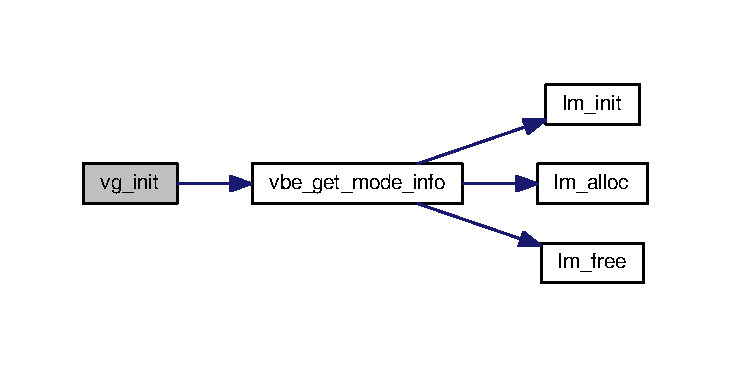
\includegraphics[width=350pt]{group__video__gr_gacef21667c79365d57a084bed994c2189_cgraph}
\end{center}
\end{figure}


\index{video\+\_\+gr@{video\+\_\+gr}!vg\+\_\+png@{vg\+\_\+png}}
\index{vg\+\_\+png@{vg\+\_\+png}!video\+\_\+gr@{video\+\_\+gr}}
\subsubsection[{\texorpdfstring{vg\+\_\+png(unsigned char $\ast$image, int width, int height, int start\+\_\+x, int start\+\_\+y)}{vg_png(unsigned char *image, int width, int height, int start_x, int start_y)}}]{\setlength{\rightskip}{0pt plus 5cm}void vg\+\_\+png (
\begin{DoxyParamCaption}
\item[{unsigned char $\ast$}]{image, }
\item[{int}]{width, }
\item[{int}]{height, }
\item[{int}]{start\+\_\+x, }
\item[{int}]{start\+\_\+y}
\end{DoxyParamCaption}
)}\hypertarget{group__video__gr_gab27465d29f462aeaf3e710695fc20594}{}\label{group__video__gr_gab27465d29f462aeaf3e710695fc20594}


Here is the call graph for this function\+:
\nopagebreak
\begin{figure}[H]
\begin{center}
\leavevmode
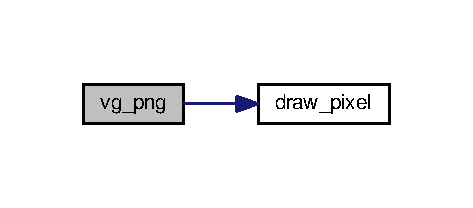
\includegraphics[width=227pt]{group__video__gr_gab27465d29f462aeaf3e710695fc20594_cgraph}
\end{center}
\end{figure}



\chapter{Class Documentation}
\hypertarget{struct____attribute____}{}\section{\+\_\+\+\_\+attribute\+\_\+\+\_\+ Struct Reference}
\label{struct____attribute____}\index{\+\_\+\+\_\+attribute\+\_\+\+\_\+@{\+\_\+\+\_\+attribute\+\_\+\+\_\+}}


{\ttfamily \#include $<$vbe.\+h$>$}

\subsection*{Public Attributes}
\begin{DoxyCompactItemize}
\item 
uint16\+\_\+t \hyperlink{struct____attribute_____a68ea99ad36679e583fa9674016e30903}{Mode\+Attributes}
\begin{DoxyCompactList}\small\item\em mode attributes \end{DoxyCompactList}\item 
uint8\+\_\+t \hyperlink{struct____attribute_____aeffe4dec59c5a757f65a97a66c812d3b}{Win\+A\+Attributes}
\begin{DoxyCompactList}\small\item\em window A attributes \end{DoxyCompactList}\item 
uint8\+\_\+t \hyperlink{struct____attribute_____ac9e21a3d7d22b24ed82be39f790b1408}{Win\+B\+Attributes}
\begin{DoxyCompactList}\small\item\em window B attributes \end{DoxyCompactList}\item 
uint16\+\_\+t \hyperlink{struct____attribute_____acc2114dbf039909e55cc3966abd3358d}{Win\+Granularity}
\begin{DoxyCompactList}\small\item\em window granularity \end{DoxyCompactList}\item 
uint16\+\_\+t \hyperlink{struct____attribute_____ad26e754fe362f3085c7ec4c0e5e75a6f}{Win\+Size}
\begin{DoxyCompactList}\small\item\em window size \end{DoxyCompactList}\item 
uint16\+\_\+t \hyperlink{struct____attribute_____a7cde26f911e3df97b7498ee139d8de12}{Win\+A\+Segment}
\begin{DoxyCompactList}\small\item\em window A start segment \end{DoxyCompactList}\item 
uint16\+\_\+t \hyperlink{struct____attribute_____a6dbaac9ee1cae36ca0c7b46559264b69}{Win\+B\+Segment}
\begin{DoxyCompactList}\small\item\em window B start segment \end{DoxyCompactList}\item 
phys\+\_\+bytes \hyperlink{struct____attribute_____aa211c2411f48f899b0bb0739ecef0b37}{Win\+Func\+Ptr}
\begin{DoxyCompactList}\small\item\em real mode/far pointer to window function \end{DoxyCompactList}\item 
uint16\+\_\+t \hyperlink{struct____attribute_____a3c9eb4b107ecee102c6e63f9054ede06}{Bytes\+Per\+Scan\+Line}
\begin{DoxyCompactList}\small\item\em bytes per scan line \end{DoxyCompactList}\item 
uint16\+\_\+t \hyperlink{struct____attribute_____abe48e2b29aa99e813a1447d22711f4f4}{X\+Resolution}
\begin{DoxyCompactList}\small\item\em horizontal resolution in pixels/characters \end{DoxyCompactList}\item 
uint16\+\_\+t \hyperlink{struct____attribute_____aa91385451d974d9c33978062e22d39e2}{Y\+Resolution}
\begin{DoxyCompactList}\small\item\em vertical resolution in pixels/characters \end{DoxyCompactList}\item 
uint8\+\_\+t \hyperlink{struct____attribute_____acac41a300563737d7849a92cd1d5c10b}{X\+Char\+Size}
\begin{DoxyCompactList}\small\item\em character cell width in pixels \end{DoxyCompactList}\item 
uint8\+\_\+t \hyperlink{struct____attribute_____acb93d86860efea5c87e3c2950f39123e}{Y\+Char\+Size}
\begin{DoxyCompactList}\small\item\em character cell height in pixels \end{DoxyCompactList}\item 
uint8\+\_\+t \hyperlink{struct____attribute_____ab1471d2f75e61117d65290da9070cf89}{Number\+Of\+Planes}
\begin{DoxyCompactList}\small\item\em number of memory planes \end{DoxyCompactList}\item 
uint8\+\_\+t \hyperlink{struct____attribute_____abd9c59af53589a54188bb57ada5c5f26}{Bits\+Per\+Pixel}
\begin{DoxyCompactList}\small\item\em bits per pixel \end{DoxyCompactList}\item 
uint8\+\_\+t \hyperlink{struct____attribute_____a59483378dd87414afcde6cb3ca93c2d8}{Number\+Of\+Banks}
\begin{DoxyCompactList}\small\item\em number of banks \end{DoxyCompactList}\item 
uint8\+\_\+t \hyperlink{struct____attribute_____a0fe34321b6dfba9e784fbbc649aa193a}{Memory\+Model}
\begin{DoxyCompactList}\small\item\em memory model type \end{DoxyCompactList}\item 
uint8\+\_\+t \hyperlink{struct____attribute_____aa1307567cbc12f9c5c724b7457be14ad}{Bank\+Size}
\begin{DoxyCompactList}\small\item\em bank size in KB \end{DoxyCompactList}\item 
uint8\+\_\+t \hyperlink{struct____attribute_____a988714bc16626547fbdc31f25dfa6470}{Number\+Of\+Image\+Pages}
\begin{DoxyCompactList}\small\item\em number of images \end{DoxyCompactList}\item 
uint8\+\_\+t \hyperlink{struct____attribute_____a8ace2dfe4814abc401442986ac8a5356}{Reserved1}
\begin{DoxyCompactList}\small\item\em reserved for page function \end{DoxyCompactList}\item 
uint8\+\_\+t \hyperlink{struct____attribute_____a9ffc14e11d6b1c80b63aba344292849e}{Red\+Mask\+Size}
\item 
uint8\+\_\+t \hyperlink{struct____attribute_____a8b5b2e458757061bce7e056f7f910dae}{Red\+Field\+Position}
\item 
uint8\+\_\+t \hyperlink{struct____attribute_____af69ef188a0f5d526ecd5f25a8d6336e3}{Green\+Mask\+Size}
\item 
uint8\+\_\+t \hyperlink{struct____attribute_____a44aab7c8026a131654e079837a95ba2b}{Green\+Field\+Position}
\item 
uint8\+\_\+t \hyperlink{struct____attribute_____ab5967602a79dcb7f0061195ffdaaa47a}{Blue\+Mask\+Size}
\item 
uint8\+\_\+t \hyperlink{struct____attribute_____ada852d5ed926757d24b5038a38e6292c}{Blue\+Field\+Position}
\item 
uint8\+\_\+t \hyperlink{struct____attribute_____a73862db83bdb9b6d31356af3cec7a5be}{Rsvd\+Mask\+Size}
\item 
uint8\+\_\+t \hyperlink{struct____attribute_____a61fb6dc07b7edbd8a3a94745336f256c}{Rsvd\+Field\+Position}
\item 
uint8\+\_\+t \hyperlink{struct____attribute_____a35fb3e1fc0dc9924bc52977b3a234f9f}{Direct\+Color\+Mode\+Info}
\item 
phys\+\_\+bytes \hyperlink{struct____attribute_____a852a4f68cfbabf08df197128e137bde6}{Phys\+Base\+Ptr}
\begin{DoxyCompactList}\small\item\em physical address for flat memory frame buffer \end{DoxyCompactList}\item 
uint8\+\_\+t \hyperlink{struct____attribute_____a534ebf7a2bdad17747cfc9cb6cc50c5c}{Reserved2} \mbox{[}4\mbox{]}
\begin{DoxyCompactList}\small\item\em Reserved -\/ always set to 0. \end{DoxyCompactList}\item 
uint8\+\_\+t \hyperlink{struct____attribute_____a9336499af9094522dbe1bfd4d43934a1}{Reserved3} \mbox{[}2\mbox{]}
\begin{DoxyCompactList}\small\item\em Reserved -\/ always set to 0. \end{DoxyCompactList}\item 
uint16\+\_\+t \hyperlink{struct____attribute_____af7036270c257deabc1ebd111faf3e3a5}{Lin\+Bytes\+Per\+Scan\+Line}
\item 
uint8\+\_\+t \hyperlink{struct____attribute_____ad5820084f2b821b85a635df8394f0d9e}{Bnk\+Number\+Of\+Image\+Pages}
\item 
uint8\+\_\+t \hyperlink{struct____attribute_____af9ba0d9902f5336bd9d044a9dee2ba42}{Lin\+Number\+Of\+Image\+Pages}
\item 
uint8\+\_\+t \hyperlink{struct____attribute_____a88a5ced225c9ef7ed6ffe33e5a39edc6}{Lin\+Red\+Mask\+Size}
\item 
uint8\+\_\+t \hyperlink{struct____attribute_____aec8d45f188ac9210b88216af83de847d}{Lin\+Red\+Field\+Position}
\item 
uint8\+\_\+t \hyperlink{struct____attribute_____a5768a84391f8a26d8a9bfd6a22d5e49d}{Lin\+Green\+Mask\+Size}
\item 
uint8\+\_\+t \hyperlink{struct____attribute_____a5571b1959950d520f2b45bb5549994e3}{Lin\+Green\+Field\+Position}
\item 
uint8\+\_\+t \hyperlink{struct____attribute_____aa2b79b8eed8d842e0db481fb1fbb9a06}{Lin\+Blue\+Mask\+Size}
\item 
uint8\+\_\+t \hyperlink{struct____attribute_____a99e6b6bdbda9f98f2823429dfd5b5685}{Lin\+Blue\+Field\+Position}
\item 
uint8\+\_\+t \hyperlink{struct____attribute_____a577b5892a22d06e230f528a62a472d1d}{Lin\+Rsvd\+Mask\+Size}
\item 
uint8\+\_\+t \hyperlink{struct____attribute_____a012126db503ad1281ae53aa41f4c96a7}{Lin\+Rsvd\+Field\+Position}
\item 
uint32\+\_\+t \hyperlink{struct____attribute_____afd81a69353c35e8b1fb9b696931f79a5}{Max\+Pixel\+Clock}
\item 
uint8\+\_\+t \hyperlink{struct____attribute_____ab859fb715f83f005dfa2f13d8b0e4ff0}{Reserved4} \mbox{[}190\mbox{]}
\end{DoxyCompactItemize}


\subsection{Detailed Description}
Packed V\+BE Mode Info Block 

\subsection{Member Data Documentation}
\index{\+\_\+\+\_\+attribute\+\_\+\+\_\+@{\+\_\+\+\_\+attribute\+\_\+\+\_\+}!Bank\+Size@{Bank\+Size}}
\index{Bank\+Size@{Bank\+Size}!\+\_\+\+\_\+attribute\+\_\+\+\_\+@{\+\_\+\+\_\+attribute\+\_\+\+\_\+}}
\subsubsection[{\texorpdfstring{Bank\+Size}{BankSize}}]{\setlength{\rightskip}{0pt plus 5cm}uint8\+\_\+t \+\_\+\+\_\+attribute\+\_\+\+\_\+\+::\+Bank\+Size}\hypertarget{struct____attribute_____aa1307567cbc12f9c5c724b7457be14ad}{}\label{struct____attribute_____aa1307567cbc12f9c5c724b7457be14ad}


bank size in KB 

\index{\+\_\+\+\_\+attribute\+\_\+\+\_\+@{\+\_\+\+\_\+attribute\+\_\+\+\_\+}!Bits\+Per\+Pixel@{Bits\+Per\+Pixel}}
\index{Bits\+Per\+Pixel@{Bits\+Per\+Pixel}!\+\_\+\+\_\+attribute\+\_\+\+\_\+@{\+\_\+\+\_\+attribute\+\_\+\+\_\+}}
\subsubsection[{\texorpdfstring{Bits\+Per\+Pixel}{BitsPerPixel}}]{\setlength{\rightskip}{0pt plus 5cm}uint8\+\_\+t \+\_\+\+\_\+attribute\+\_\+\+\_\+\+::\+Bits\+Per\+Pixel}\hypertarget{struct____attribute_____abd9c59af53589a54188bb57ada5c5f26}{}\label{struct____attribute_____abd9c59af53589a54188bb57ada5c5f26}


bits per pixel 

\index{\+\_\+\+\_\+attribute\+\_\+\+\_\+@{\+\_\+\+\_\+attribute\+\_\+\+\_\+}!Blue\+Field\+Position@{Blue\+Field\+Position}}
\index{Blue\+Field\+Position@{Blue\+Field\+Position}!\+\_\+\+\_\+attribute\+\_\+\+\_\+@{\+\_\+\+\_\+attribute\+\_\+\+\_\+}}
\subsubsection[{\texorpdfstring{Blue\+Field\+Position}{BlueFieldPosition}}]{\setlength{\rightskip}{0pt plus 5cm}uint8\+\_\+t \+\_\+\+\_\+attribute\+\_\+\+\_\+\+::\+Blue\+Field\+Position}\hypertarget{struct____attribute_____ada852d5ed926757d24b5038a38e6292c}{}\label{struct____attribute_____ada852d5ed926757d24b5038a38e6292c}
\index{\+\_\+\+\_\+attribute\+\_\+\+\_\+@{\+\_\+\+\_\+attribute\+\_\+\+\_\+}!Blue\+Mask\+Size@{Blue\+Mask\+Size}}
\index{Blue\+Mask\+Size@{Blue\+Mask\+Size}!\+\_\+\+\_\+attribute\+\_\+\+\_\+@{\+\_\+\+\_\+attribute\+\_\+\+\_\+}}
\subsubsection[{\texorpdfstring{Blue\+Mask\+Size}{BlueMaskSize}}]{\setlength{\rightskip}{0pt plus 5cm}uint8\+\_\+t \+\_\+\+\_\+attribute\+\_\+\+\_\+\+::\+Blue\+Mask\+Size}\hypertarget{struct____attribute_____ab5967602a79dcb7f0061195ffdaaa47a}{}\label{struct____attribute_____ab5967602a79dcb7f0061195ffdaaa47a}
\index{\+\_\+\+\_\+attribute\+\_\+\+\_\+@{\+\_\+\+\_\+attribute\+\_\+\+\_\+}!Bnk\+Number\+Of\+Image\+Pages@{Bnk\+Number\+Of\+Image\+Pages}}
\index{Bnk\+Number\+Of\+Image\+Pages@{Bnk\+Number\+Of\+Image\+Pages}!\+\_\+\+\_\+attribute\+\_\+\+\_\+@{\+\_\+\+\_\+attribute\+\_\+\+\_\+}}
\subsubsection[{\texorpdfstring{Bnk\+Number\+Of\+Image\+Pages}{BnkNumberOfImagePages}}]{\setlength{\rightskip}{0pt plus 5cm}uint8\+\_\+t \+\_\+\+\_\+attribute\+\_\+\+\_\+\+::\+Bnk\+Number\+Of\+Image\+Pages}\hypertarget{struct____attribute_____ad5820084f2b821b85a635df8394f0d9e}{}\label{struct____attribute_____ad5820084f2b821b85a635df8394f0d9e}
\index{\+\_\+\+\_\+attribute\+\_\+\+\_\+@{\+\_\+\+\_\+attribute\+\_\+\+\_\+}!Bytes\+Per\+Scan\+Line@{Bytes\+Per\+Scan\+Line}}
\index{Bytes\+Per\+Scan\+Line@{Bytes\+Per\+Scan\+Line}!\+\_\+\+\_\+attribute\+\_\+\+\_\+@{\+\_\+\+\_\+attribute\+\_\+\+\_\+}}
\subsubsection[{\texorpdfstring{Bytes\+Per\+Scan\+Line}{BytesPerScanLine}}]{\setlength{\rightskip}{0pt plus 5cm}uint16\+\_\+t \+\_\+\+\_\+attribute\+\_\+\+\_\+\+::\+Bytes\+Per\+Scan\+Line}\hypertarget{struct____attribute_____a3c9eb4b107ecee102c6e63f9054ede06}{}\label{struct____attribute_____a3c9eb4b107ecee102c6e63f9054ede06}


bytes per scan line 

\index{\+\_\+\+\_\+attribute\+\_\+\+\_\+@{\+\_\+\+\_\+attribute\+\_\+\+\_\+}!Direct\+Color\+Mode\+Info@{Direct\+Color\+Mode\+Info}}
\index{Direct\+Color\+Mode\+Info@{Direct\+Color\+Mode\+Info}!\+\_\+\+\_\+attribute\+\_\+\+\_\+@{\+\_\+\+\_\+attribute\+\_\+\+\_\+}}
\subsubsection[{\texorpdfstring{Direct\+Color\+Mode\+Info}{DirectColorModeInfo}}]{\setlength{\rightskip}{0pt plus 5cm}uint8\+\_\+t \+\_\+\+\_\+attribute\+\_\+\+\_\+\+::\+Direct\+Color\+Mode\+Info}\hypertarget{struct____attribute_____a35fb3e1fc0dc9924bc52977b3a234f9f}{}\label{struct____attribute_____a35fb3e1fc0dc9924bc52977b3a234f9f}
\index{\+\_\+\+\_\+attribute\+\_\+\+\_\+@{\+\_\+\+\_\+attribute\+\_\+\+\_\+}!Green\+Field\+Position@{Green\+Field\+Position}}
\index{Green\+Field\+Position@{Green\+Field\+Position}!\+\_\+\+\_\+attribute\+\_\+\+\_\+@{\+\_\+\+\_\+attribute\+\_\+\+\_\+}}
\subsubsection[{\texorpdfstring{Green\+Field\+Position}{GreenFieldPosition}}]{\setlength{\rightskip}{0pt plus 5cm}uint8\+\_\+t \+\_\+\+\_\+attribute\+\_\+\+\_\+\+::\+Green\+Field\+Position}\hypertarget{struct____attribute_____a44aab7c8026a131654e079837a95ba2b}{}\label{struct____attribute_____a44aab7c8026a131654e079837a95ba2b}
\index{\+\_\+\+\_\+attribute\+\_\+\+\_\+@{\+\_\+\+\_\+attribute\+\_\+\+\_\+}!Green\+Mask\+Size@{Green\+Mask\+Size}}
\index{Green\+Mask\+Size@{Green\+Mask\+Size}!\+\_\+\+\_\+attribute\+\_\+\+\_\+@{\+\_\+\+\_\+attribute\+\_\+\+\_\+}}
\subsubsection[{\texorpdfstring{Green\+Mask\+Size}{GreenMaskSize}}]{\setlength{\rightskip}{0pt plus 5cm}uint8\+\_\+t \+\_\+\+\_\+attribute\+\_\+\+\_\+\+::\+Green\+Mask\+Size}\hypertarget{struct____attribute_____af69ef188a0f5d526ecd5f25a8d6336e3}{}\label{struct____attribute_____af69ef188a0f5d526ecd5f25a8d6336e3}
\index{\+\_\+\+\_\+attribute\+\_\+\+\_\+@{\+\_\+\+\_\+attribute\+\_\+\+\_\+}!Lin\+Blue\+Field\+Position@{Lin\+Blue\+Field\+Position}}
\index{Lin\+Blue\+Field\+Position@{Lin\+Blue\+Field\+Position}!\+\_\+\+\_\+attribute\+\_\+\+\_\+@{\+\_\+\+\_\+attribute\+\_\+\+\_\+}}
\subsubsection[{\texorpdfstring{Lin\+Blue\+Field\+Position}{LinBlueFieldPosition}}]{\setlength{\rightskip}{0pt plus 5cm}uint8\+\_\+t \+\_\+\+\_\+attribute\+\_\+\+\_\+\+::\+Lin\+Blue\+Field\+Position}\hypertarget{struct____attribute_____a99e6b6bdbda9f98f2823429dfd5b5685}{}\label{struct____attribute_____a99e6b6bdbda9f98f2823429dfd5b5685}
\index{\+\_\+\+\_\+attribute\+\_\+\+\_\+@{\+\_\+\+\_\+attribute\+\_\+\+\_\+}!Lin\+Blue\+Mask\+Size@{Lin\+Blue\+Mask\+Size}}
\index{Lin\+Blue\+Mask\+Size@{Lin\+Blue\+Mask\+Size}!\+\_\+\+\_\+attribute\+\_\+\+\_\+@{\+\_\+\+\_\+attribute\+\_\+\+\_\+}}
\subsubsection[{\texorpdfstring{Lin\+Blue\+Mask\+Size}{LinBlueMaskSize}}]{\setlength{\rightskip}{0pt plus 5cm}uint8\+\_\+t \+\_\+\+\_\+attribute\+\_\+\+\_\+\+::\+Lin\+Blue\+Mask\+Size}\hypertarget{struct____attribute_____aa2b79b8eed8d842e0db481fb1fbb9a06}{}\label{struct____attribute_____aa2b79b8eed8d842e0db481fb1fbb9a06}
\index{\+\_\+\+\_\+attribute\+\_\+\+\_\+@{\+\_\+\+\_\+attribute\+\_\+\+\_\+}!Lin\+Bytes\+Per\+Scan\+Line@{Lin\+Bytes\+Per\+Scan\+Line}}
\index{Lin\+Bytes\+Per\+Scan\+Line@{Lin\+Bytes\+Per\+Scan\+Line}!\+\_\+\+\_\+attribute\+\_\+\+\_\+@{\+\_\+\+\_\+attribute\+\_\+\+\_\+}}
\subsubsection[{\texorpdfstring{Lin\+Bytes\+Per\+Scan\+Line}{LinBytesPerScanLine}}]{\setlength{\rightskip}{0pt plus 5cm}uint16\+\_\+t \+\_\+\+\_\+attribute\+\_\+\+\_\+\+::\+Lin\+Bytes\+Per\+Scan\+Line}\hypertarget{struct____attribute_____af7036270c257deabc1ebd111faf3e3a5}{}\label{struct____attribute_____af7036270c257deabc1ebd111faf3e3a5}
\index{\+\_\+\+\_\+attribute\+\_\+\+\_\+@{\+\_\+\+\_\+attribute\+\_\+\+\_\+}!Lin\+Green\+Field\+Position@{Lin\+Green\+Field\+Position}}
\index{Lin\+Green\+Field\+Position@{Lin\+Green\+Field\+Position}!\+\_\+\+\_\+attribute\+\_\+\+\_\+@{\+\_\+\+\_\+attribute\+\_\+\+\_\+}}
\subsubsection[{\texorpdfstring{Lin\+Green\+Field\+Position}{LinGreenFieldPosition}}]{\setlength{\rightskip}{0pt plus 5cm}uint8\+\_\+t \+\_\+\+\_\+attribute\+\_\+\+\_\+\+::\+Lin\+Green\+Field\+Position}\hypertarget{struct____attribute_____a5571b1959950d520f2b45bb5549994e3}{}\label{struct____attribute_____a5571b1959950d520f2b45bb5549994e3}
\index{\+\_\+\+\_\+attribute\+\_\+\+\_\+@{\+\_\+\+\_\+attribute\+\_\+\+\_\+}!Lin\+Green\+Mask\+Size@{Lin\+Green\+Mask\+Size}}
\index{Lin\+Green\+Mask\+Size@{Lin\+Green\+Mask\+Size}!\+\_\+\+\_\+attribute\+\_\+\+\_\+@{\+\_\+\+\_\+attribute\+\_\+\+\_\+}}
\subsubsection[{\texorpdfstring{Lin\+Green\+Mask\+Size}{LinGreenMaskSize}}]{\setlength{\rightskip}{0pt plus 5cm}uint8\+\_\+t \+\_\+\+\_\+attribute\+\_\+\+\_\+\+::\+Lin\+Green\+Mask\+Size}\hypertarget{struct____attribute_____a5768a84391f8a26d8a9bfd6a22d5e49d}{}\label{struct____attribute_____a5768a84391f8a26d8a9bfd6a22d5e49d}
\index{\+\_\+\+\_\+attribute\+\_\+\+\_\+@{\+\_\+\+\_\+attribute\+\_\+\+\_\+}!Lin\+Number\+Of\+Image\+Pages@{Lin\+Number\+Of\+Image\+Pages}}
\index{Lin\+Number\+Of\+Image\+Pages@{Lin\+Number\+Of\+Image\+Pages}!\+\_\+\+\_\+attribute\+\_\+\+\_\+@{\+\_\+\+\_\+attribute\+\_\+\+\_\+}}
\subsubsection[{\texorpdfstring{Lin\+Number\+Of\+Image\+Pages}{LinNumberOfImagePages}}]{\setlength{\rightskip}{0pt plus 5cm}uint8\+\_\+t \+\_\+\+\_\+attribute\+\_\+\+\_\+\+::\+Lin\+Number\+Of\+Image\+Pages}\hypertarget{struct____attribute_____af9ba0d9902f5336bd9d044a9dee2ba42}{}\label{struct____attribute_____af9ba0d9902f5336bd9d044a9dee2ba42}
\index{\+\_\+\+\_\+attribute\+\_\+\+\_\+@{\+\_\+\+\_\+attribute\+\_\+\+\_\+}!Lin\+Red\+Field\+Position@{Lin\+Red\+Field\+Position}}
\index{Lin\+Red\+Field\+Position@{Lin\+Red\+Field\+Position}!\+\_\+\+\_\+attribute\+\_\+\+\_\+@{\+\_\+\+\_\+attribute\+\_\+\+\_\+}}
\subsubsection[{\texorpdfstring{Lin\+Red\+Field\+Position}{LinRedFieldPosition}}]{\setlength{\rightskip}{0pt plus 5cm}uint8\+\_\+t \+\_\+\+\_\+attribute\+\_\+\+\_\+\+::\+Lin\+Red\+Field\+Position}\hypertarget{struct____attribute_____aec8d45f188ac9210b88216af83de847d}{}\label{struct____attribute_____aec8d45f188ac9210b88216af83de847d}
\index{\+\_\+\+\_\+attribute\+\_\+\+\_\+@{\+\_\+\+\_\+attribute\+\_\+\+\_\+}!Lin\+Red\+Mask\+Size@{Lin\+Red\+Mask\+Size}}
\index{Lin\+Red\+Mask\+Size@{Lin\+Red\+Mask\+Size}!\+\_\+\+\_\+attribute\+\_\+\+\_\+@{\+\_\+\+\_\+attribute\+\_\+\+\_\+}}
\subsubsection[{\texorpdfstring{Lin\+Red\+Mask\+Size}{LinRedMaskSize}}]{\setlength{\rightskip}{0pt plus 5cm}uint8\+\_\+t \+\_\+\+\_\+attribute\+\_\+\+\_\+\+::\+Lin\+Red\+Mask\+Size}\hypertarget{struct____attribute_____a88a5ced225c9ef7ed6ffe33e5a39edc6}{}\label{struct____attribute_____a88a5ced225c9ef7ed6ffe33e5a39edc6}
\index{\+\_\+\+\_\+attribute\+\_\+\+\_\+@{\+\_\+\+\_\+attribute\+\_\+\+\_\+}!Lin\+Rsvd\+Field\+Position@{Lin\+Rsvd\+Field\+Position}}
\index{Lin\+Rsvd\+Field\+Position@{Lin\+Rsvd\+Field\+Position}!\+\_\+\+\_\+attribute\+\_\+\+\_\+@{\+\_\+\+\_\+attribute\+\_\+\+\_\+}}
\subsubsection[{\texorpdfstring{Lin\+Rsvd\+Field\+Position}{LinRsvdFieldPosition}}]{\setlength{\rightskip}{0pt plus 5cm}uint8\+\_\+t \+\_\+\+\_\+attribute\+\_\+\+\_\+\+::\+Lin\+Rsvd\+Field\+Position}\hypertarget{struct____attribute_____a012126db503ad1281ae53aa41f4c96a7}{}\label{struct____attribute_____a012126db503ad1281ae53aa41f4c96a7}
\index{\+\_\+\+\_\+attribute\+\_\+\+\_\+@{\+\_\+\+\_\+attribute\+\_\+\+\_\+}!Lin\+Rsvd\+Mask\+Size@{Lin\+Rsvd\+Mask\+Size}}
\index{Lin\+Rsvd\+Mask\+Size@{Lin\+Rsvd\+Mask\+Size}!\+\_\+\+\_\+attribute\+\_\+\+\_\+@{\+\_\+\+\_\+attribute\+\_\+\+\_\+}}
\subsubsection[{\texorpdfstring{Lin\+Rsvd\+Mask\+Size}{LinRsvdMaskSize}}]{\setlength{\rightskip}{0pt plus 5cm}uint8\+\_\+t \+\_\+\+\_\+attribute\+\_\+\+\_\+\+::\+Lin\+Rsvd\+Mask\+Size}\hypertarget{struct____attribute_____a577b5892a22d06e230f528a62a472d1d}{}\label{struct____attribute_____a577b5892a22d06e230f528a62a472d1d}
\index{\+\_\+\+\_\+attribute\+\_\+\+\_\+@{\+\_\+\+\_\+attribute\+\_\+\+\_\+}!Max\+Pixel\+Clock@{Max\+Pixel\+Clock}}
\index{Max\+Pixel\+Clock@{Max\+Pixel\+Clock}!\+\_\+\+\_\+attribute\+\_\+\+\_\+@{\+\_\+\+\_\+attribute\+\_\+\+\_\+}}
\subsubsection[{\texorpdfstring{Max\+Pixel\+Clock}{MaxPixelClock}}]{\setlength{\rightskip}{0pt plus 5cm}uint32\+\_\+t \+\_\+\+\_\+attribute\+\_\+\+\_\+\+::\+Max\+Pixel\+Clock}\hypertarget{struct____attribute_____afd81a69353c35e8b1fb9b696931f79a5}{}\label{struct____attribute_____afd81a69353c35e8b1fb9b696931f79a5}
\index{\+\_\+\+\_\+attribute\+\_\+\+\_\+@{\+\_\+\+\_\+attribute\+\_\+\+\_\+}!Memory\+Model@{Memory\+Model}}
\index{Memory\+Model@{Memory\+Model}!\+\_\+\+\_\+attribute\+\_\+\+\_\+@{\+\_\+\+\_\+attribute\+\_\+\+\_\+}}
\subsubsection[{\texorpdfstring{Memory\+Model}{MemoryModel}}]{\setlength{\rightskip}{0pt plus 5cm}uint8\+\_\+t \+\_\+\+\_\+attribute\+\_\+\+\_\+\+::\+Memory\+Model}\hypertarget{struct____attribute_____a0fe34321b6dfba9e784fbbc649aa193a}{}\label{struct____attribute_____a0fe34321b6dfba9e784fbbc649aa193a}


memory model type 

\index{\+\_\+\+\_\+attribute\+\_\+\+\_\+@{\+\_\+\+\_\+attribute\+\_\+\+\_\+}!Mode\+Attributes@{Mode\+Attributes}}
\index{Mode\+Attributes@{Mode\+Attributes}!\+\_\+\+\_\+attribute\+\_\+\+\_\+@{\+\_\+\+\_\+attribute\+\_\+\+\_\+}}
\subsubsection[{\texorpdfstring{Mode\+Attributes}{ModeAttributes}}]{\setlength{\rightskip}{0pt plus 5cm}uint16\+\_\+t \+\_\+\+\_\+attribute\+\_\+\+\_\+\+::\+Mode\+Attributes}\hypertarget{struct____attribute_____a68ea99ad36679e583fa9674016e30903}{}\label{struct____attribute_____a68ea99ad36679e583fa9674016e30903}


mode attributes 

\index{\+\_\+\+\_\+attribute\+\_\+\+\_\+@{\+\_\+\+\_\+attribute\+\_\+\+\_\+}!Number\+Of\+Banks@{Number\+Of\+Banks}}
\index{Number\+Of\+Banks@{Number\+Of\+Banks}!\+\_\+\+\_\+attribute\+\_\+\+\_\+@{\+\_\+\+\_\+attribute\+\_\+\+\_\+}}
\subsubsection[{\texorpdfstring{Number\+Of\+Banks}{NumberOfBanks}}]{\setlength{\rightskip}{0pt plus 5cm}uint8\+\_\+t \+\_\+\+\_\+attribute\+\_\+\+\_\+\+::\+Number\+Of\+Banks}\hypertarget{struct____attribute_____a59483378dd87414afcde6cb3ca93c2d8}{}\label{struct____attribute_____a59483378dd87414afcde6cb3ca93c2d8}


number of banks 

\index{\+\_\+\+\_\+attribute\+\_\+\+\_\+@{\+\_\+\+\_\+attribute\+\_\+\+\_\+}!Number\+Of\+Image\+Pages@{Number\+Of\+Image\+Pages}}
\index{Number\+Of\+Image\+Pages@{Number\+Of\+Image\+Pages}!\+\_\+\+\_\+attribute\+\_\+\+\_\+@{\+\_\+\+\_\+attribute\+\_\+\+\_\+}}
\subsubsection[{\texorpdfstring{Number\+Of\+Image\+Pages}{NumberOfImagePages}}]{\setlength{\rightskip}{0pt plus 5cm}uint8\+\_\+t \+\_\+\+\_\+attribute\+\_\+\+\_\+\+::\+Number\+Of\+Image\+Pages}\hypertarget{struct____attribute_____a988714bc16626547fbdc31f25dfa6470}{}\label{struct____attribute_____a988714bc16626547fbdc31f25dfa6470}


number of images 

\index{\+\_\+\+\_\+attribute\+\_\+\+\_\+@{\+\_\+\+\_\+attribute\+\_\+\+\_\+}!Number\+Of\+Planes@{Number\+Of\+Planes}}
\index{Number\+Of\+Planes@{Number\+Of\+Planes}!\+\_\+\+\_\+attribute\+\_\+\+\_\+@{\+\_\+\+\_\+attribute\+\_\+\+\_\+}}
\subsubsection[{\texorpdfstring{Number\+Of\+Planes}{NumberOfPlanes}}]{\setlength{\rightskip}{0pt plus 5cm}uint8\+\_\+t \+\_\+\+\_\+attribute\+\_\+\+\_\+\+::\+Number\+Of\+Planes}\hypertarget{struct____attribute_____ab1471d2f75e61117d65290da9070cf89}{}\label{struct____attribute_____ab1471d2f75e61117d65290da9070cf89}


number of memory planes 

\index{\+\_\+\+\_\+attribute\+\_\+\+\_\+@{\+\_\+\+\_\+attribute\+\_\+\+\_\+}!Phys\+Base\+Ptr@{Phys\+Base\+Ptr}}
\index{Phys\+Base\+Ptr@{Phys\+Base\+Ptr}!\+\_\+\+\_\+attribute\+\_\+\+\_\+@{\+\_\+\+\_\+attribute\+\_\+\+\_\+}}
\subsubsection[{\texorpdfstring{Phys\+Base\+Ptr}{PhysBasePtr}}]{\setlength{\rightskip}{0pt plus 5cm}phys\+\_\+bytes \+\_\+\+\_\+attribute\+\_\+\+\_\+\+::\+Phys\+Base\+Ptr}\hypertarget{struct____attribute_____a852a4f68cfbabf08df197128e137bde6}{}\label{struct____attribute_____a852a4f68cfbabf08df197128e137bde6}


physical address for flat memory frame buffer 

\index{\+\_\+\+\_\+attribute\+\_\+\+\_\+@{\+\_\+\+\_\+attribute\+\_\+\+\_\+}!Red\+Field\+Position@{Red\+Field\+Position}}
\index{Red\+Field\+Position@{Red\+Field\+Position}!\+\_\+\+\_\+attribute\+\_\+\+\_\+@{\+\_\+\+\_\+attribute\+\_\+\+\_\+}}
\subsubsection[{\texorpdfstring{Red\+Field\+Position}{RedFieldPosition}}]{\setlength{\rightskip}{0pt plus 5cm}uint8\+\_\+t \+\_\+\+\_\+attribute\+\_\+\+\_\+\+::\+Red\+Field\+Position}\hypertarget{struct____attribute_____a8b5b2e458757061bce7e056f7f910dae}{}\label{struct____attribute_____a8b5b2e458757061bce7e056f7f910dae}
\index{\+\_\+\+\_\+attribute\+\_\+\+\_\+@{\+\_\+\+\_\+attribute\+\_\+\+\_\+}!Red\+Mask\+Size@{Red\+Mask\+Size}}
\index{Red\+Mask\+Size@{Red\+Mask\+Size}!\+\_\+\+\_\+attribute\+\_\+\+\_\+@{\+\_\+\+\_\+attribute\+\_\+\+\_\+}}
\subsubsection[{\texorpdfstring{Red\+Mask\+Size}{RedMaskSize}}]{\setlength{\rightskip}{0pt plus 5cm}uint8\+\_\+t \+\_\+\+\_\+attribute\+\_\+\+\_\+\+::\+Red\+Mask\+Size}\hypertarget{struct____attribute_____a9ffc14e11d6b1c80b63aba344292849e}{}\label{struct____attribute_____a9ffc14e11d6b1c80b63aba344292849e}
\index{\+\_\+\+\_\+attribute\+\_\+\+\_\+@{\+\_\+\+\_\+attribute\+\_\+\+\_\+}!Reserved1@{Reserved1}}
\index{Reserved1@{Reserved1}!\+\_\+\+\_\+attribute\+\_\+\+\_\+@{\+\_\+\+\_\+attribute\+\_\+\+\_\+}}
\subsubsection[{\texorpdfstring{Reserved1}{Reserved1}}]{\setlength{\rightskip}{0pt plus 5cm}uint8\+\_\+t \+\_\+\+\_\+attribute\+\_\+\+\_\+\+::\+Reserved1}\hypertarget{struct____attribute_____a8ace2dfe4814abc401442986ac8a5356}{}\label{struct____attribute_____a8ace2dfe4814abc401442986ac8a5356}


reserved for page function 

\index{\+\_\+\+\_\+attribute\+\_\+\+\_\+@{\+\_\+\+\_\+attribute\+\_\+\+\_\+}!Reserved2@{Reserved2}}
\index{Reserved2@{Reserved2}!\+\_\+\+\_\+attribute\+\_\+\+\_\+@{\+\_\+\+\_\+attribute\+\_\+\+\_\+}}
\subsubsection[{\texorpdfstring{Reserved2}{Reserved2}}]{\setlength{\rightskip}{0pt plus 5cm}uint8\+\_\+t \+\_\+\+\_\+attribute\+\_\+\+\_\+\+::\+Reserved2\mbox{[}4\mbox{]}}\hypertarget{struct____attribute_____a534ebf7a2bdad17747cfc9cb6cc50c5c}{}\label{struct____attribute_____a534ebf7a2bdad17747cfc9cb6cc50c5c}


Reserved -\/ always set to 0. 

\index{\+\_\+\+\_\+attribute\+\_\+\+\_\+@{\+\_\+\+\_\+attribute\+\_\+\+\_\+}!Reserved3@{Reserved3}}
\index{Reserved3@{Reserved3}!\+\_\+\+\_\+attribute\+\_\+\+\_\+@{\+\_\+\+\_\+attribute\+\_\+\+\_\+}}
\subsubsection[{\texorpdfstring{Reserved3}{Reserved3}}]{\setlength{\rightskip}{0pt plus 5cm}uint8\+\_\+t \+\_\+\+\_\+attribute\+\_\+\+\_\+\+::\+Reserved3\mbox{[}2\mbox{]}}\hypertarget{struct____attribute_____a9336499af9094522dbe1bfd4d43934a1}{}\label{struct____attribute_____a9336499af9094522dbe1bfd4d43934a1}


Reserved -\/ always set to 0. 

\index{\+\_\+\+\_\+attribute\+\_\+\+\_\+@{\+\_\+\+\_\+attribute\+\_\+\+\_\+}!Reserved4@{Reserved4}}
\index{Reserved4@{Reserved4}!\+\_\+\+\_\+attribute\+\_\+\+\_\+@{\+\_\+\+\_\+attribute\+\_\+\+\_\+}}
\subsubsection[{\texorpdfstring{Reserved4}{Reserved4}}]{\setlength{\rightskip}{0pt plus 5cm}uint8\+\_\+t \+\_\+\+\_\+attribute\+\_\+\+\_\+\+::\+Reserved4\mbox{[}190\mbox{]}}\hypertarget{struct____attribute_____ab859fb715f83f005dfa2f13d8b0e4ff0}{}\label{struct____attribute_____ab859fb715f83f005dfa2f13d8b0e4ff0}
\index{\+\_\+\+\_\+attribute\+\_\+\+\_\+@{\+\_\+\+\_\+attribute\+\_\+\+\_\+}!Rsvd\+Field\+Position@{Rsvd\+Field\+Position}}
\index{Rsvd\+Field\+Position@{Rsvd\+Field\+Position}!\+\_\+\+\_\+attribute\+\_\+\+\_\+@{\+\_\+\+\_\+attribute\+\_\+\+\_\+}}
\subsubsection[{\texorpdfstring{Rsvd\+Field\+Position}{RsvdFieldPosition}}]{\setlength{\rightskip}{0pt plus 5cm}uint8\+\_\+t \+\_\+\+\_\+attribute\+\_\+\+\_\+\+::\+Rsvd\+Field\+Position}\hypertarget{struct____attribute_____a61fb6dc07b7edbd8a3a94745336f256c}{}\label{struct____attribute_____a61fb6dc07b7edbd8a3a94745336f256c}
\index{\+\_\+\+\_\+attribute\+\_\+\+\_\+@{\+\_\+\+\_\+attribute\+\_\+\+\_\+}!Rsvd\+Mask\+Size@{Rsvd\+Mask\+Size}}
\index{Rsvd\+Mask\+Size@{Rsvd\+Mask\+Size}!\+\_\+\+\_\+attribute\+\_\+\+\_\+@{\+\_\+\+\_\+attribute\+\_\+\+\_\+}}
\subsubsection[{\texorpdfstring{Rsvd\+Mask\+Size}{RsvdMaskSize}}]{\setlength{\rightskip}{0pt plus 5cm}uint8\+\_\+t \+\_\+\+\_\+attribute\+\_\+\+\_\+\+::\+Rsvd\+Mask\+Size}\hypertarget{struct____attribute_____a73862db83bdb9b6d31356af3cec7a5be}{}\label{struct____attribute_____a73862db83bdb9b6d31356af3cec7a5be}
\index{\+\_\+\+\_\+attribute\+\_\+\+\_\+@{\+\_\+\+\_\+attribute\+\_\+\+\_\+}!Win\+A\+Attributes@{Win\+A\+Attributes}}
\index{Win\+A\+Attributes@{Win\+A\+Attributes}!\+\_\+\+\_\+attribute\+\_\+\+\_\+@{\+\_\+\+\_\+attribute\+\_\+\+\_\+}}
\subsubsection[{\texorpdfstring{Win\+A\+Attributes}{WinAAttributes}}]{\setlength{\rightskip}{0pt plus 5cm}uint8\+\_\+t \+\_\+\+\_\+attribute\+\_\+\+\_\+\+::\+Win\+A\+Attributes}\hypertarget{struct____attribute_____aeffe4dec59c5a757f65a97a66c812d3b}{}\label{struct____attribute_____aeffe4dec59c5a757f65a97a66c812d3b}


window A attributes 

\index{\+\_\+\+\_\+attribute\+\_\+\+\_\+@{\+\_\+\+\_\+attribute\+\_\+\+\_\+}!Win\+A\+Segment@{Win\+A\+Segment}}
\index{Win\+A\+Segment@{Win\+A\+Segment}!\+\_\+\+\_\+attribute\+\_\+\+\_\+@{\+\_\+\+\_\+attribute\+\_\+\+\_\+}}
\subsubsection[{\texorpdfstring{Win\+A\+Segment}{WinASegment}}]{\setlength{\rightskip}{0pt plus 5cm}uint16\+\_\+t \+\_\+\+\_\+attribute\+\_\+\+\_\+\+::\+Win\+A\+Segment}\hypertarget{struct____attribute_____a7cde26f911e3df97b7498ee139d8de12}{}\label{struct____attribute_____a7cde26f911e3df97b7498ee139d8de12}


window A start segment 

\index{\+\_\+\+\_\+attribute\+\_\+\+\_\+@{\+\_\+\+\_\+attribute\+\_\+\+\_\+}!Win\+B\+Attributes@{Win\+B\+Attributes}}
\index{Win\+B\+Attributes@{Win\+B\+Attributes}!\+\_\+\+\_\+attribute\+\_\+\+\_\+@{\+\_\+\+\_\+attribute\+\_\+\+\_\+}}
\subsubsection[{\texorpdfstring{Win\+B\+Attributes}{WinBAttributes}}]{\setlength{\rightskip}{0pt plus 5cm}uint8\+\_\+t \+\_\+\+\_\+attribute\+\_\+\+\_\+\+::\+Win\+B\+Attributes}\hypertarget{struct____attribute_____ac9e21a3d7d22b24ed82be39f790b1408}{}\label{struct____attribute_____ac9e21a3d7d22b24ed82be39f790b1408}


window B attributes 

\index{\+\_\+\+\_\+attribute\+\_\+\+\_\+@{\+\_\+\+\_\+attribute\+\_\+\+\_\+}!Win\+B\+Segment@{Win\+B\+Segment}}
\index{Win\+B\+Segment@{Win\+B\+Segment}!\+\_\+\+\_\+attribute\+\_\+\+\_\+@{\+\_\+\+\_\+attribute\+\_\+\+\_\+}}
\subsubsection[{\texorpdfstring{Win\+B\+Segment}{WinBSegment}}]{\setlength{\rightskip}{0pt plus 5cm}uint16\+\_\+t \+\_\+\+\_\+attribute\+\_\+\+\_\+\+::\+Win\+B\+Segment}\hypertarget{struct____attribute_____a6dbaac9ee1cae36ca0c7b46559264b69}{}\label{struct____attribute_____a6dbaac9ee1cae36ca0c7b46559264b69}


window B start segment 

\index{\+\_\+\+\_\+attribute\+\_\+\+\_\+@{\+\_\+\+\_\+attribute\+\_\+\+\_\+}!Win\+Func\+Ptr@{Win\+Func\+Ptr}}
\index{Win\+Func\+Ptr@{Win\+Func\+Ptr}!\+\_\+\+\_\+attribute\+\_\+\+\_\+@{\+\_\+\+\_\+attribute\+\_\+\+\_\+}}
\subsubsection[{\texorpdfstring{Win\+Func\+Ptr}{WinFuncPtr}}]{\setlength{\rightskip}{0pt plus 5cm}phys\+\_\+bytes \+\_\+\+\_\+attribute\+\_\+\+\_\+\+::\+Win\+Func\+Ptr}\hypertarget{struct____attribute_____aa211c2411f48f899b0bb0739ecef0b37}{}\label{struct____attribute_____aa211c2411f48f899b0bb0739ecef0b37}


real mode/far pointer to window function 

\index{\+\_\+\+\_\+attribute\+\_\+\+\_\+@{\+\_\+\+\_\+attribute\+\_\+\+\_\+}!Win\+Granularity@{Win\+Granularity}}
\index{Win\+Granularity@{Win\+Granularity}!\+\_\+\+\_\+attribute\+\_\+\+\_\+@{\+\_\+\+\_\+attribute\+\_\+\+\_\+}}
\subsubsection[{\texorpdfstring{Win\+Granularity}{WinGranularity}}]{\setlength{\rightskip}{0pt plus 5cm}uint16\+\_\+t \+\_\+\+\_\+attribute\+\_\+\+\_\+\+::\+Win\+Granularity}\hypertarget{struct____attribute_____acc2114dbf039909e55cc3966abd3358d}{}\label{struct____attribute_____acc2114dbf039909e55cc3966abd3358d}


window granularity 

\index{\+\_\+\+\_\+attribute\+\_\+\+\_\+@{\+\_\+\+\_\+attribute\+\_\+\+\_\+}!Win\+Size@{Win\+Size}}
\index{Win\+Size@{Win\+Size}!\+\_\+\+\_\+attribute\+\_\+\+\_\+@{\+\_\+\+\_\+attribute\+\_\+\+\_\+}}
\subsubsection[{\texorpdfstring{Win\+Size}{WinSize}}]{\setlength{\rightskip}{0pt plus 5cm}uint16\+\_\+t \+\_\+\+\_\+attribute\+\_\+\+\_\+\+::\+Win\+Size}\hypertarget{struct____attribute_____ad26e754fe362f3085c7ec4c0e5e75a6f}{}\label{struct____attribute_____ad26e754fe362f3085c7ec4c0e5e75a6f}


window size 

\index{\+\_\+\+\_\+attribute\+\_\+\+\_\+@{\+\_\+\+\_\+attribute\+\_\+\+\_\+}!X\+Char\+Size@{X\+Char\+Size}}
\index{X\+Char\+Size@{X\+Char\+Size}!\+\_\+\+\_\+attribute\+\_\+\+\_\+@{\+\_\+\+\_\+attribute\+\_\+\+\_\+}}
\subsubsection[{\texorpdfstring{X\+Char\+Size}{XCharSize}}]{\setlength{\rightskip}{0pt plus 5cm}uint8\+\_\+t \+\_\+\+\_\+attribute\+\_\+\+\_\+\+::\+X\+Char\+Size}\hypertarget{struct____attribute_____acac41a300563737d7849a92cd1d5c10b}{}\label{struct____attribute_____acac41a300563737d7849a92cd1d5c10b}


character cell width in pixels 

\index{\+\_\+\+\_\+attribute\+\_\+\+\_\+@{\+\_\+\+\_\+attribute\+\_\+\+\_\+}!X\+Resolution@{X\+Resolution}}
\index{X\+Resolution@{X\+Resolution}!\+\_\+\+\_\+attribute\+\_\+\+\_\+@{\+\_\+\+\_\+attribute\+\_\+\+\_\+}}
\subsubsection[{\texorpdfstring{X\+Resolution}{XResolution}}]{\setlength{\rightskip}{0pt plus 5cm}uint16\+\_\+t \+\_\+\+\_\+attribute\+\_\+\+\_\+\+::\+X\+Resolution}\hypertarget{struct____attribute_____abe48e2b29aa99e813a1447d22711f4f4}{}\label{struct____attribute_____abe48e2b29aa99e813a1447d22711f4f4}


horizontal resolution in pixels/characters 

\index{\+\_\+\+\_\+attribute\+\_\+\+\_\+@{\+\_\+\+\_\+attribute\+\_\+\+\_\+}!Y\+Char\+Size@{Y\+Char\+Size}}
\index{Y\+Char\+Size@{Y\+Char\+Size}!\+\_\+\+\_\+attribute\+\_\+\+\_\+@{\+\_\+\+\_\+attribute\+\_\+\+\_\+}}
\subsubsection[{\texorpdfstring{Y\+Char\+Size}{YCharSize}}]{\setlength{\rightskip}{0pt plus 5cm}uint8\+\_\+t \+\_\+\+\_\+attribute\+\_\+\+\_\+\+::\+Y\+Char\+Size}\hypertarget{struct____attribute_____acb93d86860efea5c87e3c2950f39123e}{}\label{struct____attribute_____acb93d86860efea5c87e3c2950f39123e}


character cell height in pixels 

\index{\+\_\+\+\_\+attribute\+\_\+\+\_\+@{\+\_\+\+\_\+attribute\+\_\+\+\_\+}!Y\+Resolution@{Y\+Resolution}}
\index{Y\+Resolution@{Y\+Resolution}!\+\_\+\+\_\+attribute\+\_\+\+\_\+@{\+\_\+\+\_\+attribute\+\_\+\+\_\+}}
\subsubsection[{\texorpdfstring{Y\+Resolution}{YResolution}}]{\setlength{\rightskip}{0pt plus 5cm}uint16\+\_\+t \+\_\+\+\_\+attribute\+\_\+\+\_\+\+::\+Y\+Resolution}\hypertarget{struct____attribute_____aa91385451d974d9c33978062e22d39e2}{}\label{struct____attribute_____aa91385451d974d9c33978062e22d39e2}


vertical resolution in pixels/characters 



The documentation for this struct was generated from the following file\+:\begin{DoxyCompactItemize}
\item 
\hyperlink{vbe_8h}{vbe.\+h}\end{DoxyCompactItemize}

\hypertarget{structBike}{}\section{Bike Struct Reference}
\label{structBike}\index{Bike@{Bike}}


{\ttfamily \#include $<$bike.\+h$>$}

\subsection*{Public Attributes}
\begin{DoxyCompactItemize}
\item 
int \hyperlink{group__Bike_ga01cdf583ace46bc4e576c42b54ee628a}{initial\+\_\+x\+\_\+pos}
\item 
int \hyperlink{group__Bike_ga74f0f95635444a7570225a75f3a22056}{initial\+\_\+y\+\_\+pos}
\item 
int \hyperlink{group__Bike_ga9a5251a8d520f2ce0fc0e34dd7325a23}{direction}
\item 
int \hyperlink{group__Bike_ga3187c35b871d499fb88aca98de35282a}{head\+\_\+x\+\_\+pos}
\item 
int \hyperlink{group__Bike_ga48e90acd4f7eceb4ea0921f9a8b89f98}{head\+\_\+y\+\_\+pos}
\item 
unsigned long \hyperlink{group__Bike_ga7ba066e0787d8b239b8cb16775db0eac}{color}
\end{DoxyCompactItemize}


The documentation for this struct was generated from the following file\+:\begin{DoxyCompactItemize}
\item 
\hyperlink{bike_8h}{bike.\+h}\end{DoxyCompactItemize}

\hypertarget{structMenu}{}\section{Menu Struct Reference}
\label{structMenu}\index{Menu@{Menu}}


{\ttfamily \#include $<$menu.\+h$>$}

\subsection*{Public Attributes}
\begin{DoxyCompactItemize}
\item 
int \hyperlink{structMenu_a457588a82fea9415b58c5b9ee2595e88}{done}
\item 
unsigned char $\ast$ \hyperlink{structMenu_ae1afb1a4c1a48995dbc99aba8cb3ea09}{background}
\item 
int \hyperlink{structMenu_a58782cb93b5c0be925192ec69430abff}{background\+\_\+width}
\item 
int \hyperlink{structMenu_a9766ba80e9f48d5ca685572724be1a1f}{background\+\_\+height}
\item 
unsigned char $\ast$ \hyperlink{structMenu_a97c8de98a5b43b75e8a049db832427e3}{play}
\item 
int \hyperlink{structMenu_a5ffb3bd78cd87f2d26c09b274cb33caf}{play\+\_\+width}
\item 
int \hyperlink{structMenu_a88a30a9449606bab297bffab5818aad7}{play\+\_\+height}
\item 
unsigned char $\ast$ \hyperlink{structMenu_a99635834abf927c6f5a1e48d7aa443fd}{bwinner}
\item 
int \hyperlink{structMenu_acb0ab046c68de9fb392b7f4ba139c9ed}{bwinner\+\_\+width}
\item 
int \hyperlink{structMenu_ae7eb58473d40dc9d1c76c987fadafe0e}{bwinner\+\_\+height}
\item 
unsigned char $\ast$ \hyperlink{structMenu_aee41aa16055cd2c8ea7cb289d8011300}{wwinner}
\item 
int \hyperlink{structMenu_a3b16162ce3451366bdd585c3ddcca9bb}{wwinner\+\_\+width}
\item 
int \hyperlink{structMenu_ad6e879577aed24c8628f7041874ee244}{wwinner\+\_\+height}
\item 
unsigned char $\ast$ \hyperlink{structMenu_a56b38d2255ea43c1625f9d828fee9a28}{exit}
\item 
int \hyperlink{structMenu_a1f1abb83a7eda64961d0ab106758070b}{exit\+\_\+width}
\item 
int \hyperlink{structMenu_a7bfc348718a60afb1172985576d47d62}{exit\+\_\+height}
\item 
\hyperlink{group__Menu_gab99074a1f6b7e8ff7730342913aae3a3}{Menu\+Action} \hyperlink{structMenu_a01fc9d0084bc760f9d1e66462a8a75b7}{action}
\end{DoxyCompactItemize}


\subsection{Member Data Documentation}
\index{Menu@{Menu}!action@{action}}
\index{action@{action}!Menu@{Menu}}
\subsubsection[{\texorpdfstring{action}{action}}]{\setlength{\rightskip}{0pt plus 5cm}{\bf Menu\+Action} Menu\+::action}\hypertarget{structMenu_a01fc9d0084bc760f9d1e66462a8a75b7}{}\label{structMenu_a01fc9d0084bc760f9d1e66462a8a75b7}
indicates what to do when the state \hyperlink{structMenu}{Menu} is done \index{Menu@{Menu}!background@{background}}
\index{background@{background}!Menu@{Menu}}
\subsubsection[{\texorpdfstring{background}{background}}]{\setlength{\rightskip}{0pt plus 5cm}unsigned char$\ast$ Menu\+::background}\hypertarget{structMenu_ae1afb1a4c1a48995dbc99aba8cb3ea09}{}\label{structMenu_ae1afb1a4c1a48995dbc99aba8cb3ea09}
pointer to the play button image \index{Menu@{Menu}!background\+\_\+height@{background\+\_\+height}}
\index{background\+\_\+height@{background\+\_\+height}!Menu@{Menu}}
\subsubsection[{\texorpdfstring{background\+\_\+height}{background_height}}]{\setlength{\rightskip}{0pt plus 5cm}int Menu\+::background\+\_\+height}\hypertarget{structMenu_a9766ba80e9f48d5ca685572724be1a1f}{}\label{structMenu_a9766ba80e9f48d5ca685572724be1a1f}
\index{Menu@{Menu}!background\+\_\+width@{background\+\_\+width}}
\index{background\+\_\+width@{background\+\_\+width}!Menu@{Menu}}
\subsubsection[{\texorpdfstring{background\+\_\+width}{background_width}}]{\setlength{\rightskip}{0pt plus 5cm}int Menu\+::background\+\_\+width}\hypertarget{structMenu_a58782cb93b5c0be925192ec69430abff}{}\label{structMenu_a58782cb93b5c0be925192ec69430abff}
\index{Menu@{Menu}!bwinner@{bwinner}}
\index{bwinner@{bwinner}!Menu@{Menu}}
\subsubsection[{\texorpdfstring{bwinner}{bwinner}}]{\setlength{\rightskip}{0pt plus 5cm}unsigned char$\ast$ Menu\+::bwinner}\hypertarget{structMenu_a99635834abf927c6f5a1e48d7aa443fd}{}\label{structMenu_a99635834abf927c6f5a1e48d7aa443fd}
\index{Menu@{Menu}!bwinner\+\_\+height@{bwinner\+\_\+height}}
\index{bwinner\+\_\+height@{bwinner\+\_\+height}!Menu@{Menu}}
\subsubsection[{\texorpdfstring{bwinner\+\_\+height}{bwinner_height}}]{\setlength{\rightskip}{0pt plus 5cm}int Menu\+::bwinner\+\_\+height}\hypertarget{structMenu_ae7eb58473d40dc9d1c76c987fadafe0e}{}\label{structMenu_ae7eb58473d40dc9d1c76c987fadafe0e}
\index{Menu@{Menu}!bwinner\+\_\+width@{bwinner\+\_\+width}}
\index{bwinner\+\_\+width@{bwinner\+\_\+width}!Menu@{Menu}}
\subsubsection[{\texorpdfstring{bwinner\+\_\+width}{bwinner_width}}]{\setlength{\rightskip}{0pt plus 5cm}int Menu\+::bwinner\+\_\+width}\hypertarget{structMenu_acb0ab046c68de9fb392b7f4ba139c9ed}{}\label{structMenu_acb0ab046c68de9fb392b7f4ba139c9ed}
\index{Menu@{Menu}!done@{done}}
\index{done@{done}!Menu@{Menu}}
\subsubsection[{\texorpdfstring{done}{done}}]{\setlength{\rightskip}{0pt plus 5cm}int Menu\+::done}\hypertarget{structMenu_a457588a82fea9415b58c5b9ee2595e88}{}\label{structMenu_a457588a82fea9415b58c5b9ee2595e88}
1 change state, 0 otherwise \index{Menu@{Menu}!exit@{exit}}
\index{exit@{exit}!Menu@{Menu}}
\subsubsection[{\texorpdfstring{exit}{exit}}]{\setlength{\rightskip}{0pt plus 5cm}unsigned char$\ast$ Menu\+::exit}\hypertarget{structMenu_a56b38d2255ea43c1625f9d828fee9a28}{}\label{structMenu_a56b38d2255ea43c1625f9d828fee9a28}
pointer to the exit button image \index{Menu@{Menu}!exit\+\_\+height@{exit\+\_\+height}}
\index{exit\+\_\+height@{exit\+\_\+height}!Menu@{Menu}}
\subsubsection[{\texorpdfstring{exit\+\_\+height}{exit_height}}]{\setlength{\rightskip}{0pt plus 5cm}int Menu\+::exit\+\_\+height}\hypertarget{structMenu_a7bfc348718a60afb1172985576d47d62}{}\label{structMenu_a7bfc348718a60afb1172985576d47d62}
\index{Menu@{Menu}!exit\+\_\+width@{exit\+\_\+width}}
\index{exit\+\_\+width@{exit\+\_\+width}!Menu@{Menu}}
\subsubsection[{\texorpdfstring{exit\+\_\+width}{exit_width}}]{\setlength{\rightskip}{0pt plus 5cm}int Menu\+::exit\+\_\+width}\hypertarget{structMenu_a1f1abb83a7eda64961d0ab106758070b}{}\label{structMenu_a1f1abb83a7eda64961d0ab106758070b}
\index{Menu@{Menu}!play@{play}}
\index{play@{play}!Menu@{Menu}}
\subsubsection[{\texorpdfstring{play}{play}}]{\setlength{\rightskip}{0pt plus 5cm}unsigned char$\ast$ Menu\+::play}\hypertarget{structMenu_a97c8de98a5b43b75e8a049db832427e3}{}\label{structMenu_a97c8de98a5b43b75e8a049db832427e3}
pointer to the play button image \index{Menu@{Menu}!play\+\_\+height@{play\+\_\+height}}
\index{play\+\_\+height@{play\+\_\+height}!Menu@{Menu}}
\subsubsection[{\texorpdfstring{play\+\_\+height}{play_height}}]{\setlength{\rightskip}{0pt plus 5cm}int Menu\+::play\+\_\+height}\hypertarget{structMenu_a88a30a9449606bab297bffab5818aad7}{}\label{structMenu_a88a30a9449606bab297bffab5818aad7}
\index{Menu@{Menu}!play\+\_\+width@{play\+\_\+width}}
\index{play\+\_\+width@{play\+\_\+width}!Menu@{Menu}}
\subsubsection[{\texorpdfstring{play\+\_\+width}{play_width}}]{\setlength{\rightskip}{0pt plus 5cm}int Menu\+::play\+\_\+width}\hypertarget{structMenu_a5ffb3bd78cd87f2d26c09b274cb33caf}{}\label{structMenu_a5ffb3bd78cd87f2d26c09b274cb33caf}
\index{Menu@{Menu}!wwinner@{wwinner}}
\index{wwinner@{wwinner}!Menu@{Menu}}
\subsubsection[{\texorpdfstring{wwinner}{wwinner}}]{\setlength{\rightskip}{0pt plus 5cm}unsigned char$\ast$ Menu\+::wwinner}\hypertarget{structMenu_aee41aa16055cd2c8ea7cb289d8011300}{}\label{structMenu_aee41aa16055cd2c8ea7cb289d8011300}
\index{Menu@{Menu}!wwinner\+\_\+height@{wwinner\+\_\+height}}
\index{wwinner\+\_\+height@{wwinner\+\_\+height}!Menu@{Menu}}
\subsubsection[{\texorpdfstring{wwinner\+\_\+height}{wwinner_height}}]{\setlength{\rightskip}{0pt plus 5cm}int Menu\+::wwinner\+\_\+height}\hypertarget{structMenu_ad6e879577aed24c8628f7041874ee244}{}\label{structMenu_ad6e879577aed24c8628f7041874ee244}
\index{Menu@{Menu}!wwinner\+\_\+width@{wwinner\+\_\+width}}
\index{wwinner\+\_\+width@{wwinner\+\_\+width}!Menu@{Menu}}
\subsubsection[{\texorpdfstring{wwinner\+\_\+width}{wwinner_width}}]{\setlength{\rightskip}{0pt plus 5cm}int Menu\+::wwinner\+\_\+width}\hypertarget{structMenu_a3b16162ce3451366bdd585c3ddcca9bb}{}\label{structMenu_a3b16162ce3451366bdd585c3ddcca9bb}


The documentation for this struct was generated from the following file\+:\begin{DoxyCompactItemize}
\item 
\hyperlink{menu_8h}{menu.\+h}\end{DoxyCompactItemize}

\hypertarget{structmmap__t}{}\section{mmap\+\_\+t Struct Reference}
\label{structmmap__t}\index{mmap\+\_\+t@{mmap\+\_\+t}}


{\ttfamily \#include $<$lmlib.\+h$>$}

\subsection*{Public Attributes}
\begin{DoxyCompactItemize}
\item 
phys\+\_\+bytes \hyperlink{group__lmlib_gaa6ac1ee0e0fadea4a4f85b48c8359ae4}{phys}
\begin{DoxyCompactList}\small\item\em physical address \end{DoxyCompactList}\item 
void $\ast$ \hyperlink{group__lmlib_ga4de93144fb3ffbceb9bd1f3009d6d98c}{virtual}
\begin{DoxyCompactList}\small\item\em virtual address \end{DoxyCompactList}\item 
unsigned long \hyperlink{group__lmlib_gaf1cdc5384a402fddf33f400a5e1e5e45}{size}
\begin{DoxyCompactList}\small\item\em size of memory region \end{DoxyCompactList}\end{DoxyCompactItemize}


\subsection{Detailed Description}
Struct that keeps info regarding the mapping of physical memory to virtual memory 

The documentation for this struct was generated from the following file\+:\begin{DoxyCompactItemize}
\item 
\hyperlink{lmlib_8h}{lmlib.\+h}\end{DoxyCompactItemize}

\hypertarget{structMouse}{}\section{Mouse Struct Reference}
\label{structMouse}\index{Mouse@{Mouse}}


{\ttfamily \#include $<$mouse.\+h$>$}

\subsection*{Public Attributes}
\begin{DoxyCompactItemize}
\item 
int \hyperlink{group__Mouse_ga136eea114b70f46392b89cc3779d4291}{x}
\item 
int \hyperlink{group__Mouse_ga4a29b1c18faaa2fbe39ff985ba9d6737}{y}
\item 
int \hyperlink{group__Mouse_ga1fc496df2223cb17437b296acbe02e50}{packet\+\_\+idx}
\item 
int \hyperlink{group__Mouse_ga64798c8dfb1b60b4ce76bc9859719077}{complete\+\_\+packet}
\item 
unsigned long \hyperlink{group__Mouse_ga8bfb0c35eb14423f5086a355d52dc733}{packet} \mbox{[}3\mbox{]}
\item 
int \hyperlink{group__Mouse_ga401d046e1cad0fad3908120ab85b9396}{left\+Button\+Down}
\item 
int \hyperlink{group__Mouse_ga9a74cd5fb66c4936d44a72962df7830c}{left\+Button\+Released}
\item 
int \hyperlink{group__Mouse_gad3b4a3a6fd6d53630bdf7aa81d74f744}{draw}
\end{DoxyCompactItemize}


The documentation for this struct was generated from the following file\+:\begin{DoxyCompactItemize}
\item 
\hyperlink{mouse_8h}{mouse.\+h}\end{DoxyCompactItemize}

\hypertarget{structstbi__io__callbacks}{}\section{stbi\+\_\+io\+\_\+callbacks Struct Reference}
\label{structstbi__io__callbacks}\index{stbi\+\_\+io\+\_\+callbacks@{stbi\+\_\+io\+\_\+callbacks}}


{\ttfamily \#include $<$stb\+\_\+image.\+h$>$}

\subsection*{Public Attributes}
\begin{DoxyCompactItemize}
\item 
int($\ast$ \hyperlink{structstbi__io__callbacks_a623e46b3a2a019611601409926283a88}{read} )(void $\ast$user, char $\ast$data, int size)
\item 
void($\ast$ \hyperlink{structstbi__io__callbacks_a257aac5480a90a6c4b8fbe86c1b01068}{skip} )(void $\ast$user, int n)
\item 
int($\ast$ \hyperlink{structstbi__io__callbacks_a319639db2f76e715eed7a7a974136832}{eof} )(void $\ast$user)
\end{DoxyCompactItemize}


\subsection{Member Data Documentation}
\index{stbi\+\_\+io\+\_\+callbacks@{stbi\+\_\+io\+\_\+callbacks}!eof@{eof}}
\index{eof@{eof}!stbi\+\_\+io\+\_\+callbacks@{stbi\+\_\+io\+\_\+callbacks}}
\subsubsection[{\texorpdfstring{eof}{eof}}]{\setlength{\rightskip}{0pt plus 5cm}int($\ast$ stbi\+\_\+io\+\_\+callbacks\+::eof) (void $\ast$user)}\hypertarget{structstbi__io__callbacks_a319639db2f76e715eed7a7a974136832}{}\label{structstbi__io__callbacks_a319639db2f76e715eed7a7a974136832}
\index{stbi\+\_\+io\+\_\+callbacks@{stbi\+\_\+io\+\_\+callbacks}!read@{read}}
\index{read@{read}!stbi\+\_\+io\+\_\+callbacks@{stbi\+\_\+io\+\_\+callbacks}}
\subsubsection[{\texorpdfstring{read}{read}}]{\setlength{\rightskip}{0pt plus 5cm}int($\ast$ stbi\+\_\+io\+\_\+callbacks\+::read) (void $\ast$user, char $\ast$data, int size)}\hypertarget{structstbi__io__callbacks_a623e46b3a2a019611601409926283a88}{}\label{structstbi__io__callbacks_a623e46b3a2a019611601409926283a88}
\index{stbi\+\_\+io\+\_\+callbacks@{stbi\+\_\+io\+\_\+callbacks}!skip@{skip}}
\index{skip@{skip}!stbi\+\_\+io\+\_\+callbacks@{stbi\+\_\+io\+\_\+callbacks}}
\subsubsection[{\texorpdfstring{skip}{skip}}]{\setlength{\rightskip}{0pt plus 5cm}void($\ast$ stbi\+\_\+io\+\_\+callbacks\+::skip) (void $\ast$user, int n)}\hypertarget{structstbi__io__callbacks_a257aac5480a90a6c4b8fbe86c1b01068}{}\label{structstbi__io__callbacks_a257aac5480a90a6c4b8fbe86c1b01068}


The documentation for this struct was generated from the following file\+:\begin{DoxyCompactItemize}
\item 
\hyperlink{stb__image_8h}{stb\+\_\+image.\+h}\end{DoxyCompactItemize}

\chapter{File Documentation}
\hypertarget{bike_8c}{}\section{bike.\+c File Reference}
\label{bike_8c}\index{bike.\+c@{bike.\+c}}
{\ttfamily \#include $<$stdio.\+h$>$}\\*
{\ttfamily \#include $<$string.\+h$>$}\\*
{\ttfamily \#include \char`\"{}bike.\+h\char`\"{}}\\*
{\ttfamily \#include \char`\"{}i8042.\+h\char`\"{}}\\*
Include dependency graph for bike.\+c\+:
\nopagebreak
\begin{figure}[H]
\begin{center}
\leavevmode
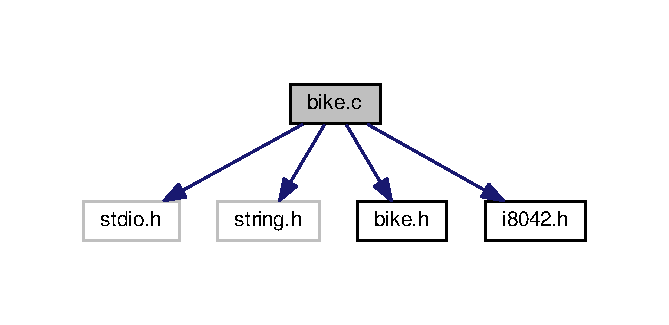
\includegraphics[width=321pt]{bike_8c__incl}
\end{center}
\end{figure}
\subsection*{Functions}
\begin{DoxyCompactItemize}
\item 
int \hyperlink{group__Bike_ga9d5bd9dd5a4b9347fa04fb0a47e7b138}{get\+InitialX} (\hyperlink{structBike}{Bike} bike)
\begin{DoxyCompactList}\small\item\em gets Initial X position \end{DoxyCompactList}\item 
int \hyperlink{group__Bike_ga2d556c34524f8fe950a96aa665aaffe8}{get\+InitialY} (\hyperlink{structBike}{Bike} bike)
\begin{DoxyCompactList}\small\item\em gets Initial Y position \end{DoxyCompactList}\item 
int \hyperlink{group__Bike_ga8d48f7de63dc2a17f3eac8b3e96f9b12}{get\+Direction} (\hyperlink{structBike}{Bike} bike)
\begin{DoxyCompactList}\small\item\em gets bike direction \end{DoxyCompactList}\item 
int \hyperlink{group__Bike_gaf4691615a2b7398e9c3b4ae2f93553e0}{get\+HeadX} (\hyperlink{structBike}{Bike} bike)
\begin{DoxyCompactList}\small\item\em gets Head X position \end{DoxyCompactList}\item 
int \hyperlink{group__Bike_gaafe273e5e247e3efd463e232686328d6}{get\+HeadY} (\hyperlink{structBike}{Bike} bike)
\begin{DoxyCompactList}\small\item\em gets Head Y position \end{DoxyCompactList}\item 
unsigned long \hyperlink{group__Bike_ga04fad9ee3b40712d1fde03fc5441ea73}{getcolor} (\hyperlink{structBike}{Bike} bike)
\begin{DoxyCompactList}\small\item\em gets the bike color \end{DoxyCompactList}\item 
void \hyperlink{group__Bike_ga0310311d1c88668900502c150b52120b}{set\+Direction} (\hyperlink{structBike}{Bike} $\ast$bike, int dir)
\begin{DoxyCompactList}\small\item\em sets the bike direction \end{DoxyCompactList}\item 
void \hyperlink{group__Bike_gadd2170ef6cbb83a919f06cf9c971c9a5}{move\+Head} (\hyperlink{structBike}{Bike} $\ast$bike, int speed)
\begin{DoxyCompactList}\small\item\em gets the bike color \end{DoxyCompactList}\end{DoxyCompactItemize}

\hypertarget{bike_8h}{}\section{bike.\+h File Reference}
\label{bike_8h}\index{bike.\+h@{bike.\+h}}
This graph shows which files directly or indirectly include this file\+:
\nopagebreak
\begin{figure}[H]
\begin{center}
\leavevmode
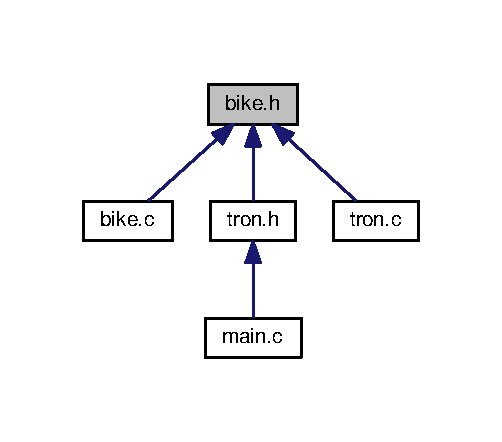
\includegraphics[width=241pt]{bike_8h__dep__incl}
\end{center}
\end{figure}
\subsection*{Classes}
\begin{DoxyCompactItemize}
\item 
struct \hyperlink{structBike}{Bike}
\end{DoxyCompactItemize}
\subsection*{Typedefs}
\begin{DoxyCompactItemize}
\item 
typedef struct \hyperlink{structBike}{Bike} \hyperlink{group__Bike_ga85f4cbf9698a8ed38ad74f4e2d71341e}{Bike}
\end{DoxyCompactItemize}
\subsection*{Functions}
\begin{DoxyCompactItemize}
\item 
int \hyperlink{group__Bike_ga9d5bd9dd5a4b9347fa04fb0a47e7b138}{get\+InitialX} (struct \hyperlink{structBike}{Bike} bike)
\begin{DoxyCompactList}\small\item\em gets Initial X position \end{DoxyCompactList}\item 
int \hyperlink{group__Bike_ga2d556c34524f8fe950a96aa665aaffe8}{get\+InitialY} (struct \hyperlink{structBike}{Bike} bike)
\begin{DoxyCompactList}\small\item\em gets Initial Y position \end{DoxyCompactList}\item 
int \hyperlink{group__Bike_ga8d48f7de63dc2a17f3eac8b3e96f9b12}{get\+Direction} (struct \hyperlink{structBike}{Bike} bike)
\begin{DoxyCompactList}\small\item\em gets bike direction \end{DoxyCompactList}\item 
int \hyperlink{group__Bike_gaf4691615a2b7398e9c3b4ae2f93553e0}{get\+HeadX} (struct \hyperlink{structBike}{Bike} bike)
\begin{DoxyCompactList}\small\item\em gets Head X position \end{DoxyCompactList}\item 
int \hyperlink{group__Bike_gaafe273e5e247e3efd463e232686328d6}{get\+HeadY} (struct \hyperlink{structBike}{Bike} bike)
\begin{DoxyCompactList}\small\item\em gets Head Y position \end{DoxyCompactList}\item 
unsigned long \hyperlink{group__Bike_ga04fad9ee3b40712d1fde03fc5441ea73}{getcolor} (struct \hyperlink{structBike}{Bike} bike)
\begin{DoxyCompactList}\small\item\em gets the bike color \end{DoxyCompactList}\item 
void \hyperlink{group__Bike_ga0310311d1c88668900502c150b52120b}{set\+Direction} (\hyperlink{structBike}{Bike} $\ast$bike, int dir)
\begin{DoxyCompactList}\small\item\em sets the bike direction \end{DoxyCompactList}\item 
void \hyperlink{group__Bike_gadd2170ef6cbb83a919f06cf9c971c9a5}{move\+Head} (\hyperlink{structBike}{Bike} $\ast$bike, int speed)
\begin{DoxyCompactList}\small\item\em gets the bike color \end{DoxyCompactList}\end{DoxyCompactItemize}

\hypertarget{i8042_8h}{}\section{i8042.\+h File Reference}
\label{i8042_8h}\index{i8042.\+h@{i8042.\+h}}
This graph shows which files directly or indirectly include this file\+:
\nopagebreak
\begin{figure}[H]
\begin{center}
\leavevmode
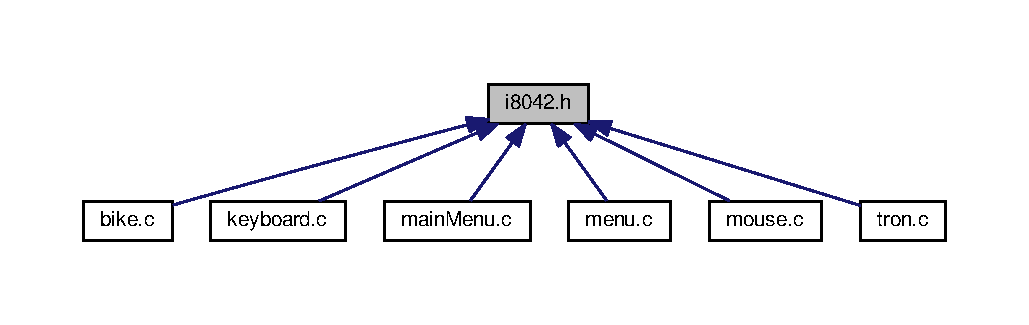
\includegraphics[width=350pt]{i8042_8h__dep__incl}
\end{center}
\end{figure}
\subsection*{Macros}
\begin{DoxyCompactItemize}
\item 
\#define \hyperlink{group__i8042_ga3a8ea58898cb58fc96013383d39f482c}{B\+IT}(n)~(0x01$<$$<$(n))
\item 
\#define \hyperlink{group__i8042_ga1a522aa19bcb695a9df30032a893bee3}{D\+E\+L\+A\+Y\+\_\+\+US}~20000
\item 
\#define \hyperlink{group__i8042_ga45ba202b05caf39795aeca91b0ae547e}{T\+I\+M\+E\+O\+UT}~4
\item 
\#define \hyperlink{group__i8042_ga16c5827f043d82f87c726c2d4369c11d}{K\+B\+C\+\_\+\+I\+RQ}~1
\begin{DoxyCompactList}\small\item\em K\+BC I\+RQ line. \end{DoxyCompactList}\item 
\#define \hyperlink{group__i8042_ga85964cb90343bb1a029b1d1b4229f910}{M\+O\+U\+S\+E\+\_\+\+I\+RQ}~12
\item 
\#define \hyperlink{group__i8042_ga89c4d098b53809674457b1660b1af780}{S\+T\+A\+T\+\_\+\+R\+EG}~0x64
\item 
\#define \hyperlink{group__i8042_ga6d57c7927a10f638c83046b52c8caac9}{K\+B\+C\+\_\+\+C\+M\+D\+\_\+\+R\+EG}~0x64
\item 
\#define \hyperlink{group__i8042_gacfb42dde389e8ca36ab267002fbf5c6a}{O\+U\+T\+\_\+\+B\+UF}~0x60
\item 
\#define \hyperlink{group__i8042_ga783be5698cf07b1daaf126ef89c19063}{I\+N\+\_\+\+B\+UF}~0x60
\item 
\#define \hyperlink{group__i8042_ga45967c9e25447ba853cf6fb4ac545fe6}{O\+BF}~\hyperlink{video_8h_a3a8ea58898cb58fc96013383d39f482c}{B\+IT}(0)
\item 
\#define \hyperlink{group__i8042_ga3c48b10907056351582baf9f6478598e}{I\+BF}~\hyperlink{video_8h_a3a8ea58898cb58fc96013383d39f482c}{B\+IT}(1)
\item 
\#define \hyperlink{group__i8042_ga307ab71673e26ec42b28a3bca05d4cb5}{P\+A\+R\+\_\+\+E\+RR}~\hyperlink{video_8h_a3a8ea58898cb58fc96013383d39f482c}{B\+IT}(7)
\item 
\#define \hyperlink{group__i8042_gad16f61e2bf70f6c7685e826224ed177f}{T\+O\+\_\+\+E\+RR}~\hyperlink{video_8h_a3a8ea58898cb58fc96013383d39f482c}{B\+IT}(6)
\item 
\#define \hyperlink{group__i8042_gad6ff09b5058171ce69f6485dbef6bfaa}{B\+R\+E\+A\+K\+C\+O\+DE}~\hyperlink{video_8h_a3a8ea58898cb58fc96013383d39f482c}{B\+IT}(7)
\item 
\#define \hyperlink{group__i8042_ga77c789e6ff7b6f33ac32ba84d3983ca4}{B\+R\+E\+A\+K\+C\+O\+D\+E\+\_\+\+E\+SC}~0x81
\item 
\#define \hyperlink{group__i8042_gab9da23ad538a1a1a68466865ac73f9b8}{T\+O\+W\+\_\+\+B\+Y\+T\+E\+\_\+\+C\+O\+DE}~0x\+E0
\item 
\#define \hyperlink{group__i8042_gaa7a45554686b9abe54443a4a80e8d2f5}{M\+A\+K\+E\+C\+O\+D\+E\+\_\+A}~0x1E
\item 
\#define \hyperlink{group__i8042_ga48a460d951bb61b2aa11903c8e817b6c}{M\+A\+K\+E\+C\+O\+D\+E\+\_\+W}~0x11
\item 
\#define \hyperlink{group__i8042_ga248870237f8cc9a4e73683480d2cfae3}{M\+A\+K\+E\+C\+O\+D\+E\+\_\+S}~0x1F
\item 
\#define \hyperlink{group__i8042_ga2c181b340e0f7986f6ea695164558fc8}{M\+A\+K\+E\+C\+O\+D\+E\+\_\+D}~0x20
\item 
\#define \hyperlink{group__i8042_ga2a701bb9a46d001c52ff40857c50daf1}{M\+A\+K\+E\+C\+O\+D\+E\+\_\+\+U\+P\+\_\+\+N\+U\+M\+P\+A\+D8}~0x48
\item 
\#define \hyperlink{group__i8042_ga820a37037cac38b3147934bdbe601843}{M\+A\+K\+E\+C\+O\+D\+E\+\_\+\+L\+E\+F\+T\+\_\+\+N\+U\+M\+P\+A\+D4}~0x4B
\item 
\#define \hyperlink{group__i8042_ga58501b39296e524f307c139e2b13b77e}{M\+A\+K\+E\+C\+O\+D\+E\+\_\+\+D\+O\+W\+N\+\_\+\+N\+U\+M\+P\+A\+D2}~0x50
\item 
\#define \hyperlink{group__i8042_gac8a539e1de5071da15f4cd6f94aba242}{M\+A\+K\+E\+C\+O\+D\+E\+\_\+\+R\+I\+G\+H\+T\+\_\+\+N\+U\+M\+P\+A\+D6}~0x4D
\item 
\#define \hyperlink{group__i8042_ga305ee86129081b404b151c64293566e7}{R\+E\+A\+D\+\_\+\+C\+O\+M\+M\+A\+N\+D\+\_\+\+B\+Y\+TE}~0x20
\item 
\#define \hyperlink{group__i8042_ga4680153f26a3244682a2e2e01e57e318}{W\+R\+I\+T\+E\+\_\+\+C\+O\+M\+M\+A\+N\+D\+\_\+\+B\+Y\+TE}~0x60
\item 
\#define \hyperlink{group__i8042_ga11095772a492a95192ea75373df94b65}{B\+Y\+T\+E\+\_\+\+T\+O\+\_\+\+M\+O\+U\+SE}~0x\+D4
\item 
\#define \hyperlink{group__i8042_gae70fc1a5ba1238a43c0f5b07740ab438}{E\+N\+A\+B\+L\+E\+\_\+\+M\+O\+U\+S\+E\+\_\+\+I\+NT}~0x47
\item 
\#define \hyperlink{group__i8042_ga1c22608f41bd715500d0333001079a8a}{E\+N\+A\+B\+L\+E\+\_\+\+D\+A\+T\+A\+\_\+\+R\+E\+P\+O\+RT}~0x\+F4
\item 
\#define \hyperlink{group__i8042_gad374b510092499b5961d3771abf9c66e}{D\+I\+S\+A\+B\+L\+E\+\_\+\+D\+A\+T\+A\+\_\+\+R\+E\+P\+O\+RT}~0x\+F5
\item 
\#define \hyperlink{group__i8042_gaabf49b4a4d8ad72d202c8a7197058e35}{S\+E\+T\+\_\+\+S\+T\+R\+E\+A\+M\+\_\+\+M\+O\+DE}~0x\+EA
\item 
\#define \hyperlink{group__i8042_ga19a57d9d2eafd32ee130c0f526906719}{S\+E\+T\+\_\+\+R\+E\+M\+O\+T\+E\+\_\+\+M\+O\+DE}~0x\+F0
\item 
\#define \hyperlink{group__i8042_ga8d406d5aff787991429e62cfd9bac721}{R\+E\+A\+D\+\_\+\+D\+A\+TA}~0x\+EB
\item 
\#define \hyperlink{group__i8042_ga6f6489887e08bff4887d0bc5dcf214d8}{A\+CK}~0x\+FA
\item 
\#define \hyperlink{group__i8042_ga958518a45b12053ae33606ee7cb68a55}{N\+A\+CK}~0x\+FE
\item 
\#define \hyperlink{group__i8042_ga8fe83ac76edc595f6b98cd4a4127aed5}{E\+R\+R\+OR}~0x\+FC
\item 
\#define \hyperlink{group__i8042_gacc55daa58d88a3612f2ef74a6abbe97f}{LB}~\hyperlink{video_8h_a3a8ea58898cb58fc96013383d39f482c}{B\+IT}(0)
\item 
\#define \hyperlink{group__i8042_ga171160a766f85c8816b898ed24d28408}{RB}~\hyperlink{video_8h_a3a8ea58898cb58fc96013383d39f482c}{B\+IT}(1)
\item 
\#define \hyperlink{group__i8042_gaa6b38d492364d98453284934ed7caee9}{MB}~\hyperlink{video_8h_a3a8ea58898cb58fc96013383d39f482c}{B\+IT}(2)
\item 
\#define \hyperlink{group__i8042_ga22a4873e9adebfc22650f6776375cce6}{X\+S\+I\+GN}~\hyperlink{video_8h_a3a8ea58898cb58fc96013383d39f482c}{B\+IT}(4)
\item 
\#define \hyperlink{group__i8042_gaf4bf97e57d9aadf00d2ec881727cccef}{Y\+S\+I\+GN}~\hyperlink{video_8h_a3a8ea58898cb58fc96013383d39f482c}{B\+IT}(5)
\item 
\#define \hyperlink{group__i8042_gac3172c891b25dafed9ced2476aa03cf1}{X\+O\+VF}~\hyperlink{video_8h_a3a8ea58898cb58fc96013383d39f482c}{B\+IT}(6)
\item 
\#define \hyperlink{group__i8042_ga08deb639aef83c70892a364261b09133}{Y\+O\+VF}~\hyperlink{video_8h_a3a8ea58898cb58fc96013383d39f482c}{B\+IT}(7)
\item 
\#define \hyperlink{group__i8042_ga79d10e672abb49ad63eeaa8aaef57c38}{B\+L\+UE}~0x0B
\item 
\#define \hyperlink{group__i8042_ga87b537f5fa5c109d3c05c13d6b18f382}{W\+H\+I\+TE}~0x3F
\item 
\#define \hyperlink{group__i8042_ga1965eaca47dbf3f87acdafc2208f04eb}{UP}~1
\item 
\#define \hyperlink{group__i8042_ga80fb826a684cf3f0d306b22aa100ddac}{R\+I\+G\+HT}~2
\item 
\#define \hyperlink{group__i8042_ga4193cd1c8c2e6ebd0e056fa2364a663f}{D\+O\+WN}~3
\item 
\#define \hyperlink{group__i8042_ga437ef08681e7210d6678427030446a54}{L\+E\+FT}~4
\end{DoxyCompactItemize}

\hypertarget{i8254_8h}{}\section{i8254.\+h File Reference}
\label{i8254_8h}\index{i8254.\+h@{i8254.\+h}}
This graph shows which files directly or indirectly include this file\+:
\nopagebreak
\begin{figure}[H]
\begin{center}
\leavevmode
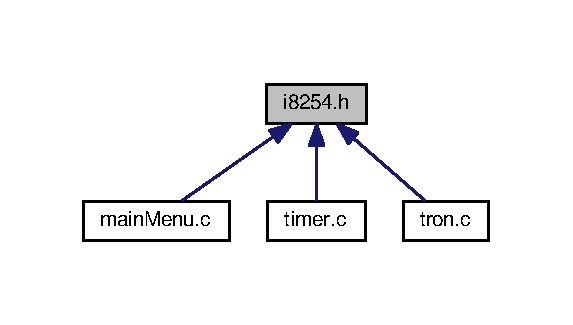
\includegraphics[width=275pt]{i8254_8h__dep__incl}
\end{center}
\end{figure}
\subsection*{Macros}
\begin{DoxyCompactItemize}
\item 
\#define \hyperlink{group__i8254_gacf926951944b6cf370b7229ebd50dd8b}{T\+I\+M\+E\+R\+\_\+\+F\+R\+EQ}~1193182
\begin{DoxyCompactList}\small\item\em clock frequency for timer in PC and AT \end{DoxyCompactList}\item 
\#define \hyperlink{group__i8254_ga12949f80c4101a3d1f40ebfc202b4914}{T\+I\+M\+E\+R0\+\_\+\+D\+E\+F\+A\+U\+L\+T\+\_\+\+F\+R\+E\+Q\+U\+E\+N\+CY}~60
\item 
\#define \hyperlink{group__i8254_ga3a8ea58898cb58fc96013383d39f482c}{B\+IT}(n)~(0x01$<$$<$(n))
\item 
\#define \hyperlink{group__i8254_ga30bf84c312af248cb81bb224e09f9ba8}{T\+I\+M\+E\+R0\+\_\+\+I\+RQ}~0
\begin{DoxyCompactList}\small\item\em Timer 0 I\+RQ line. \end{DoxyCompactList}\item 
\#define \hyperlink{group__i8254_gacc9ff9df4a9674a1ce9ba08fc4a4679e}{T\+I\+M\+E\+R\+\_\+0}~0x40
\begin{DoxyCompactList}\small\item\em Timer 0 count register. \end{DoxyCompactList}\item 
\#define \hyperlink{group__i8254_gac62c99c2a9289891c1b83052242cca49}{T\+I\+M\+E\+R\+\_\+1}~0x41
\begin{DoxyCompactList}\small\item\em Timer 1 count register. \end{DoxyCompactList}\item 
\#define \hyperlink{group__i8254_ga1f34f18ad0ab8cace46b615773b48735}{T\+I\+M\+E\+R\+\_\+2}~0x42
\begin{DoxyCompactList}\small\item\em Timer 2 count register. \end{DoxyCompactList}\item 
\#define \hyperlink{group__i8254_ga282832448fb0281ef53d243c1cd48491}{T\+I\+M\+E\+R\+\_\+\+C\+T\+RL}~0x43
\begin{DoxyCompactList}\small\item\em Control register. \end{DoxyCompactList}\item 
\#define \hyperlink{group__i8254_ga51b3a5e3d4811ca063fe25e35560ab40}{S\+P\+E\+A\+K\+E\+R\+\_\+\+C\+T\+RL}~0x61
\begin{DoxyCompactList}\small\item\em Register for speaker control. \end{DoxyCompactList}\item 
\#define \hyperlink{group__i8254_ga6a4822642d40c248435692324a818010}{T\+I\+M\+E\+R\+\_\+\+S\+E\+L0}~0x00
\begin{DoxyCompactList}\small\item\em Control Word for Timer 0. \end{DoxyCompactList}\item 
\#define \hyperlink{group__i8254_ga8349623fd8d99f9cc5d8ae29d78594fc}{T\+I\+M\+E\+R\+\_\+\+S\+E\+L1}~\hyperlink{video_8h_a3a8ea58898cb58fc96013383d39f482c}{B\+IT}(6)
\begin{DoxyCompactList}\small\item\em Control Word for Timer 1. \end{DoxyCompactList}\item 
\#define \hyperlink{group__i8254_ga142a255de0dbc48aeabd45fc10c33672}{T\+I\+M\+E\+R\+\_\+\+S\+E\+L2}~\hyperlink{video_8h_a3a8ea58898cb58fc96013383d39f482c}{B\+IT}(7)
\begin{DoxyCompactList}\small\item\em Control Word for Timer 2. \end{DoxyCompactList}\item 
\#define \hyperlink{group__i8254_ga4c2eecbfb96744a9c2af71dba75ecb18}{T\+I\+M\+E\+R\+\_\+\+R\+B\+\_\+\+C\+MD}~(\hyperlink{video_8h_a3a8ea58898cb58fc96013383d39f482c}{B\+IT}(7)$\vert$\hyperlink{video_8h_a3a8ea58898cb58fc96013383d39f482c}{B\+IT}(6))
\begin{DoxyCompactList}\small\item\em Read Back Command. \end{DoxyCompactList}\item 
\#define \hyperlink{group__i8254_gac18cb814ebd0d67235392c330e0e3504}{T\+I\+M\+E\+R\+\_\+\+L\+SB}~\hyperlink{video_8h_a3a8ea58898cb58fc96013383d39f482c}{B\+IT}(4)
\begin{DoxyCompactList}\small\item\em Initialize Counter L\+SB only. \end{DoxyCompactList}\item 
\#define \hyperlink{group__i8254_ga2a8a6d363c612d756cd8d78480f7cd04}{T\+I\+M\+E\+R\+\_\+\+M\+SB}~\hyperlink{video_8h_a3a8ea58898cb58fc96013383d39f482c}{B\+IT}(5)
\begin{DoxyCompactList}\small\item\em Initialize Counter M\+SB only. \end{DoxyCompactList}\item 
\#define \hyperlink{group__i8254_ga8c0f1933323274c765e23837e4fbc8c7}{T\+I\+M\+E\+R\+\_\+\+L\+S\+B\+\_\+\+M\+SB}~(\hyperlink{group__i8254_gac18cb814ebd0d67235392c330e0e3504}{T\+I\+M\+E\+R\+\_\+\+L\+SB} $\vert$ \hyperlink{group__i8254_ga2a8a6d363c612d756cd8d78480f7cd04}{T\+I\+M\+E\+R\+\_\+\+M\+SB})
\begin{DoxyCompactList}\small\item\em Initialize L\+SB first and M\+SB afterwards. \end{DoxyCompactList}\item 
\#define \hyperlink{group__i8254_ga4745cbf21da3d3fea5dbb080b2b73bac}{T\+I\+M\+E\+R\+\_\+\+S\+Q\+R\+\_\+\+W\+A\+VE}~(\hyperlink{video_8h_a3a8ea58898cb58fc96013383d39f482c}{B\+IT}(2)$\vert$\hyperlink{video_8h_a3a8ea58898cb58fc96013383d39f482c}{B\+IT}(1))
\begin{DoxyCompactList}\small\item\em Mode 3\+: square wave generator. \end{DoxyCompactList}\item 
\#define \hyperlink{group__i8254_ga5d4449e0fa1cf4a4d107a48a04a1265f}{T\+I\+M\+E\+R\+\_\+\+R\+A\+T\+E\+\_\+\+G\+EN}~\hyperlink{video_8h_a3a8ea58898cb58fc96013383d39f482c}{B\+IT}(2)
\begin{DoxyCompactList}\small\item\em Mode 2\+: rate generator. \end{DoxyCompactList}\item 
\#define \hyperlink{group__i8254_ga3a806d58a6b0423e5777dd471833e04d}{T\+I\+M\+E\+R\+\_\+\+M\+O\+D\+E\+\_\+\+F\+I\+VE}~(\hyperlink{video_8h_a3a8ea58898cb58fc96013383d39f482c}{B\+IT}(3)$\vert$\hyperlink{video_8h_a3a8ea58898cb58fc96013383d39f482c}{B\+IT}(1)) /$\ast$Mode 5$\ast$/
\item 
\#define \hyperlink{group__i8254_gad8bbac3f9bcc1835c3f65921bbe768dc}{T\+I\+M\+E\+R\+\_\+\+M\+O\+D\+E\+\_\+\+F\+O\+UR}~\hyperlink{video_8h_a3a8ea58898cb58fc96013383d39f482c}{B\+IT}(3) /$\ast$Mode 4$\ast$/
\item 
\#define \hyperlink{group__i8254_ga892f1f8bb1173306481a9c1ce5cfcd10}{T\+I\+M\+E\+R\+\_\+\+M\+O\+D\+E\+\_\+\+O\+NE}~\hyperlink{video_8h_a3a8ea58898cb58fc96013383d39f482c}{B\+IT}(1) /$\ast$Mode 1$\ast$/
\item 
\#define \hyperlink{group__i8254_ga325b992a371d5d981c4eceff42fa5956}{T\+I\+M\+E\+R\+\_\+\+B\+CD}~0x01
\begin{DoxyCompactList}\small\item\em Count in B\+CD. \end{DoxyCompactList}\item 
\#define \hyperlink{group__i8254_gad2913dcf2f91453317bd035589ac0a7d}{T\+I\+M\+E\+R\+\_\+\+B\+IN}~0x00
\begin{DoxyCompactList}\small\item\em Count in binary. \end{DoxyCompactList}\item 
\#define \hyperlink{group__i8254_ga6c248216df24b5e9d907d126d80bd195}{T\+I\+M\+E\+R\+\_\+\+R\+B\+\_\+\+C\+O\+U\+N\+T\+\_\+}~\hyperlink{video_8h_a3a8ea58898cb58fc96013383d39f482c}{B\+IT}(5)
\item 
\#define \hyperlink{group__i8254_ga08b4952bb7058684a3f8f66be04dd45e}{T\+I\+M\+E\+R\+\_\+\+R\+B\+\_\+\+S\+T\+A\+T\+U\+S\+\_\+}~\hyperlink{video_8h_a3a8ea58898cb58fc96013383d39f482c}{B\+IT}(4)
\item 
\#define \hyperlink{group__i8254_gaf598b17740e07842a0545af512714711}{T\+I\+M\+E\+R\+\_\+\+R\+B\+\_\+\+S\+EL}(n)~\hyperlink{video_8h_a3a8ea58898cb58fc96013383d39f482c}{B\+IT}((n)+1)
\end{DoxyCompactItemize}

\hypertarget{keyboard_8c}{}\section{keyboard.\+c File Reference}
\label{keyboard_8c}\index{keyboard.\+c@{keyboard.\+c}}
{\ttfamily \#include $<$minix/syslib.\+h$>$}\\*
{\ttfamily \#include $<$minix/drivers.\+h$>$}\\*
{\ttfamily \#include $<$minix/com.\+h$>$}\\*
{\ttfamily \#include $<$minix/sysutil.\+h$>$}\\*
{\ttfamily \#include \char`\"{}keyboard.\+h\char`\"{}}\\*
{\ttfamily \#include \char`\"{}i8042.\+h\char`\"{}}\\*
Include dependency graph for keyboard.\+c\+:
\nopagebreak
\begin{figure}[H]
\begin{center}
\leavevmode
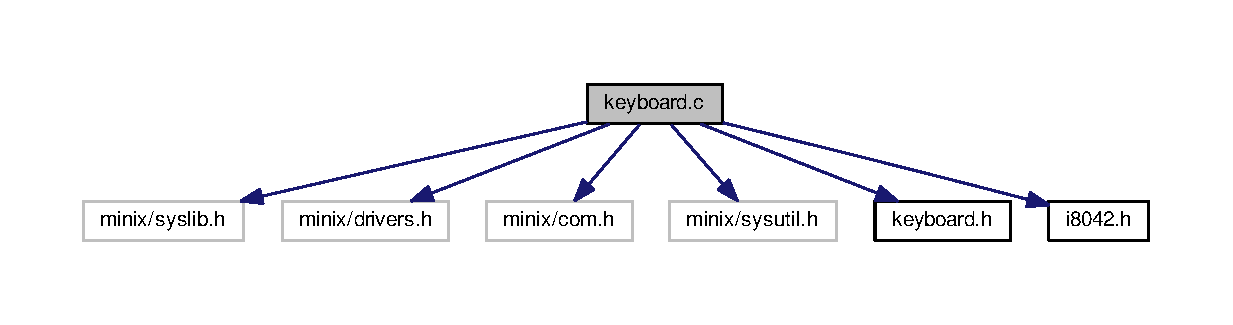
\includegraphics[width=350pt]{keyboard_8c__incl}
\end{center}
\end{figure}
\subsection*{Functions}
\begin{DoxyCompactItemize}
\item 
int \hyperlink{group__Keyboard_ga9a4aaf9e5cee256ad4af890935f2a976}{kbc\+\_\+subscribe\+\_\+int} (void)
\begin{DoxyCompactList}\small\item\em Subscribes and enables K\+BC interrupts. \end{DoxyCompactList}\item 
int \hyperlink{group__Keyboard_ga0e945987c2233f1c30a645ec5fc750c1}{kbc\+\_\+unsubscribe\+\_\+int} ()
\begin{DoxyCompactList}\small\item\em Unsubscribes K\+BC interrupts. \end{DoxyCompactList}\item 
int \hyperlink{group__Keyboard_ga0028905df4260d371b30e92f547c712a}{kbc\+\_\+read} ()
\begin{DoxyCompactList}\small\item\em Read O\+U\+T\+P\+UT B\+U\+F\+F\+ER (0x60) \end{DoxyCompactList}\item 
int \hyperlink{group__Keyboard_gaed40b556eb233ac6f329eb8396192b6f}{kbc\+\_\+write} (unsigned long porto, unsigned long cmd)
\begin{DoxyCompactList}\small\item\em write command to the kbc First reads status comand byte \end{DoxyCompactList}\end{DoxyCompactItemize}
\subsection*{Variables}
\begin{DoxyCompactItemize}
\item 
static int \hyperlink{keyboard_8c_a0bac4ccb7ceeff54a0b16bf899694f06}{kbc\+\_\+hook} = 1
\end{DoxyCompactItemize}


\subsection{Variable Documentation}
\index{keyboard.\+c@{keyboard.\+c}!kbc\+\_\+hook@{kbc\+\_\+hook}}
\index{kbc\+\_\+hook@{kbc\+\_\+hook}!keyboard.\+c@{keyboard.\+c}}
\subsubsection[{\texorpdfstring{kbc\+\_\+hook}{kbc_hook}}]{\setlength{\rightskip}{0pt plus 5cm}int kbc\+\_\+hook = 1\hspace{0.3cm}{\ttfamily [static]}}\hypertarget{keyboard_8c_a0bac4ccb7ceeff54a0b16bf899694f06}{}\label{keyboard_8c_a0bac4ccb7ceeff54a0b16bf899694f06}

\hypertarget{keyboard_8h}{}\section{keyboard.\+h File Reference}
\label{keyboard_8h}\index{keyboard.\+h@{keyboard.\+h}}
This graph shows which files directly or indirectly include this file\+:
\nopagebreak
\begin{figure}[H]
\begin{center}
\leavevmode
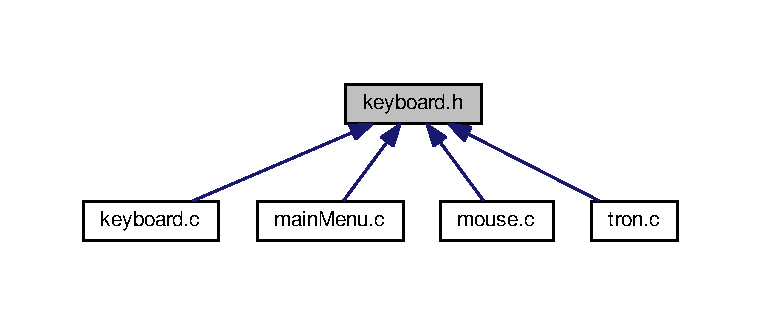
\includegraphics[width=350pt]{keyboard_8h__dep__incl}
\end{center}
\end{figure}
\subsection*{Functions}
\begin{DoxyCompactItemize}
\item 
int \hyperlink{group__Keyboard_ga9a4aaf9e5cee256ad4af890935f2a976}{kbc\+\_\+subscribe\+\_\+int} (void)
\begin{DoxyCompactList}\small\item\em Subscribes and enables K\+BC interrupts. \end{DoxyCompactList}\item 
int \hyperlink{group__Keyboard_ga0e945987c2233f1c30a645ec5fc750c1}{kbc\+\_\+unsubscribe\+\_\+int} ()
\begin{DoxyCompactList}\small\item\em Unsubscribes K\+BC interrupts. \end{DoxyCompactList}\item 
int \hyperlink{group__Keyboard_ga0028905df4260d371b30e92f547c712a}{kbc\+\_\+read} ()
\begin{DoxyCompactList}\small\item\em Read O\+U\+T\+P\+UT B\+U\+F\+F\+ER (0x60) \end{DoxyCompactList}\item 
int \hyperlink{group__Keyboard_gaed40b556eb233ac6f329eb8396192b6f}{kbc\+\_\+write} (unsigned long porto, unsigned long cmd)
\begin{DoxyCompactList}\small\item\em write command to the kbc First reads status comand byte \end{DoxyCompactList}\end{DoxyCompactItemize}

\hypertarget{lmlib_8h}{}\section{lmlib.\+h File Reference}
\label{lmlib_8h}\index{lmlib.\+h@{lmlib.\+h}}
This graph shows which files directly or indirectly include this file\+:
\nopagebreak
\begin{figure}[H]
\begin{center}
\leavevmode
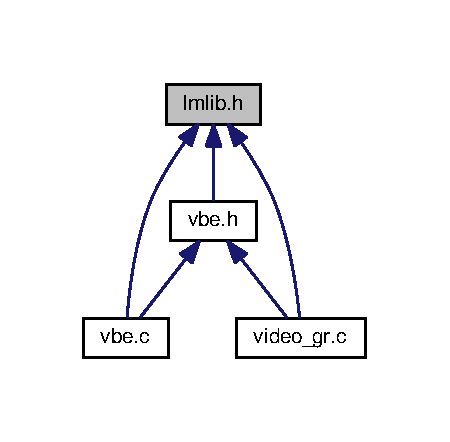
\includegraphics[width=216pt]{lmlib_8h__dep__incl}
\end{center}
\end{figure}
\subsection*{Classes}
\begin{DoxyCompactItemize}
\item 
struct \hyperlink{structmmap__t}{mmap\+\_\+t}
\end{DoxyCompactItemize}
\subsection*{Functions}
\begin{DoxyCompactItemize}
\item 
void $\ast$ \hyperlink{group__lmlib_ga00a9c17c01e794a6bfc80fc5c6ab1ed1}{lm\+\_\+init} (void)
\begin{DoxyCompactList}\small\item\em Initializes the low memory area, the region up to the 1 M\+Byte physical address, by mapping it on the process\textquotesingle{} physical memory address. \end{DoxyCompactList}\item 
void $\ast$ \hyperlink{group__lmlib_gae45d971ce2ffcf4dc2677eba033a92cd}{lm\+\_\+alloc} (unsigned long size, \hyperlink{structmmap__t}{mmap\+\_\+t} $\ast$map)
\begin{DoxyCompactList}\small\item\em Allocates a memory block in low memory area with the specified size. \end{DoxyCompactList}\item 
void \hyperlink{group__lmlib_ga73e89d9c297b7390021fb545513579c6}{lm\+\_\+free} (\hyperlink{structmmap__t}{mmap\+\_\+t} $\ast$map)
\begin{DoxyCompactList}\small\item\em Frees a memory block in the low memory area, previously allocated using \hyperlink{group__lmlib_gae45d971ce2ffcf4dc2677eba033a92cd}{lm\+\_\+alloc()} \end{DoxyCompactList}\end{DoxyCompactItemize}

\hypertarget{main_8c}{}\section{main.\+c File Reference}
\label{main_8c}\index{main.\+c@{main.\+c}}
{\ttfamily \#include $<$minix/drivers.\+h$>$}\\*
{\ttfamily \#include $<$limits.\+h$>$}\\*
{\ttfamily \#include $<$string.\+h$>$}\\*
{\ttfamily \#include $<$errno.\+h$>$}\\*
{\ttfamily \#include $<$stdio.\+h$>$}\\*
{\ttfamily \#include $<$stdint.\+h$>$}\\*
{\ttfamily \#include \char`\"{}tron.\+h\char`\"{}}\\*
{\ttfamily \#include \char`\"{}main\+Menu.\+h\char`\"{}}\\*
Include dependency graph for main.\+c\+:
\nopagebreak
\begin{figure}[H]
\begin{center}
\leavevmode
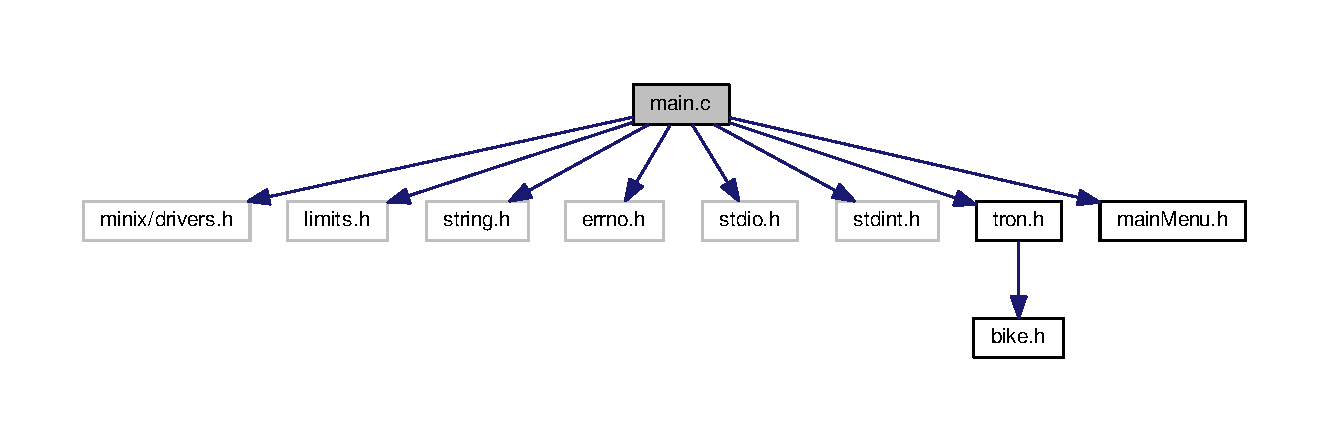
\includegraphics[width=350pt]{main_8c__incl}
\end{center}
\end{figure}
\subsection*{Functions}
\begin{DoxyCompactItemize}
\item 
int \hyperlink{main_8c_ae66f6b31b5ad750f1fe042a706a4e3d4}{main} ()
\end{DoxyCompactItemize}


\subsection{Function Documentation}
\index{main.\+c@{main.\+c}!main@{main}}
\index{main@{main}!main.\+c@{main.\+c}}
\subsubsection[{\texorpdfstring{main()}{main()}}]{\setlength{\rightskip}{0pt plus 5cm}int main (
\begin{DoxyParamCaption}
{}
\end{DoxyParamCaption}
)}\hypertarget{main_8c_ae66f6b31b5ad750f1fe042a706a4e3d4}{}\label{main_8c_ae66f6b31b5ad750f1fe042a706a4e3d4}


Here is the call graph for this function\+:
\nopagebreak
\begin{figure}[H]
\begin{center}
\leavevmode
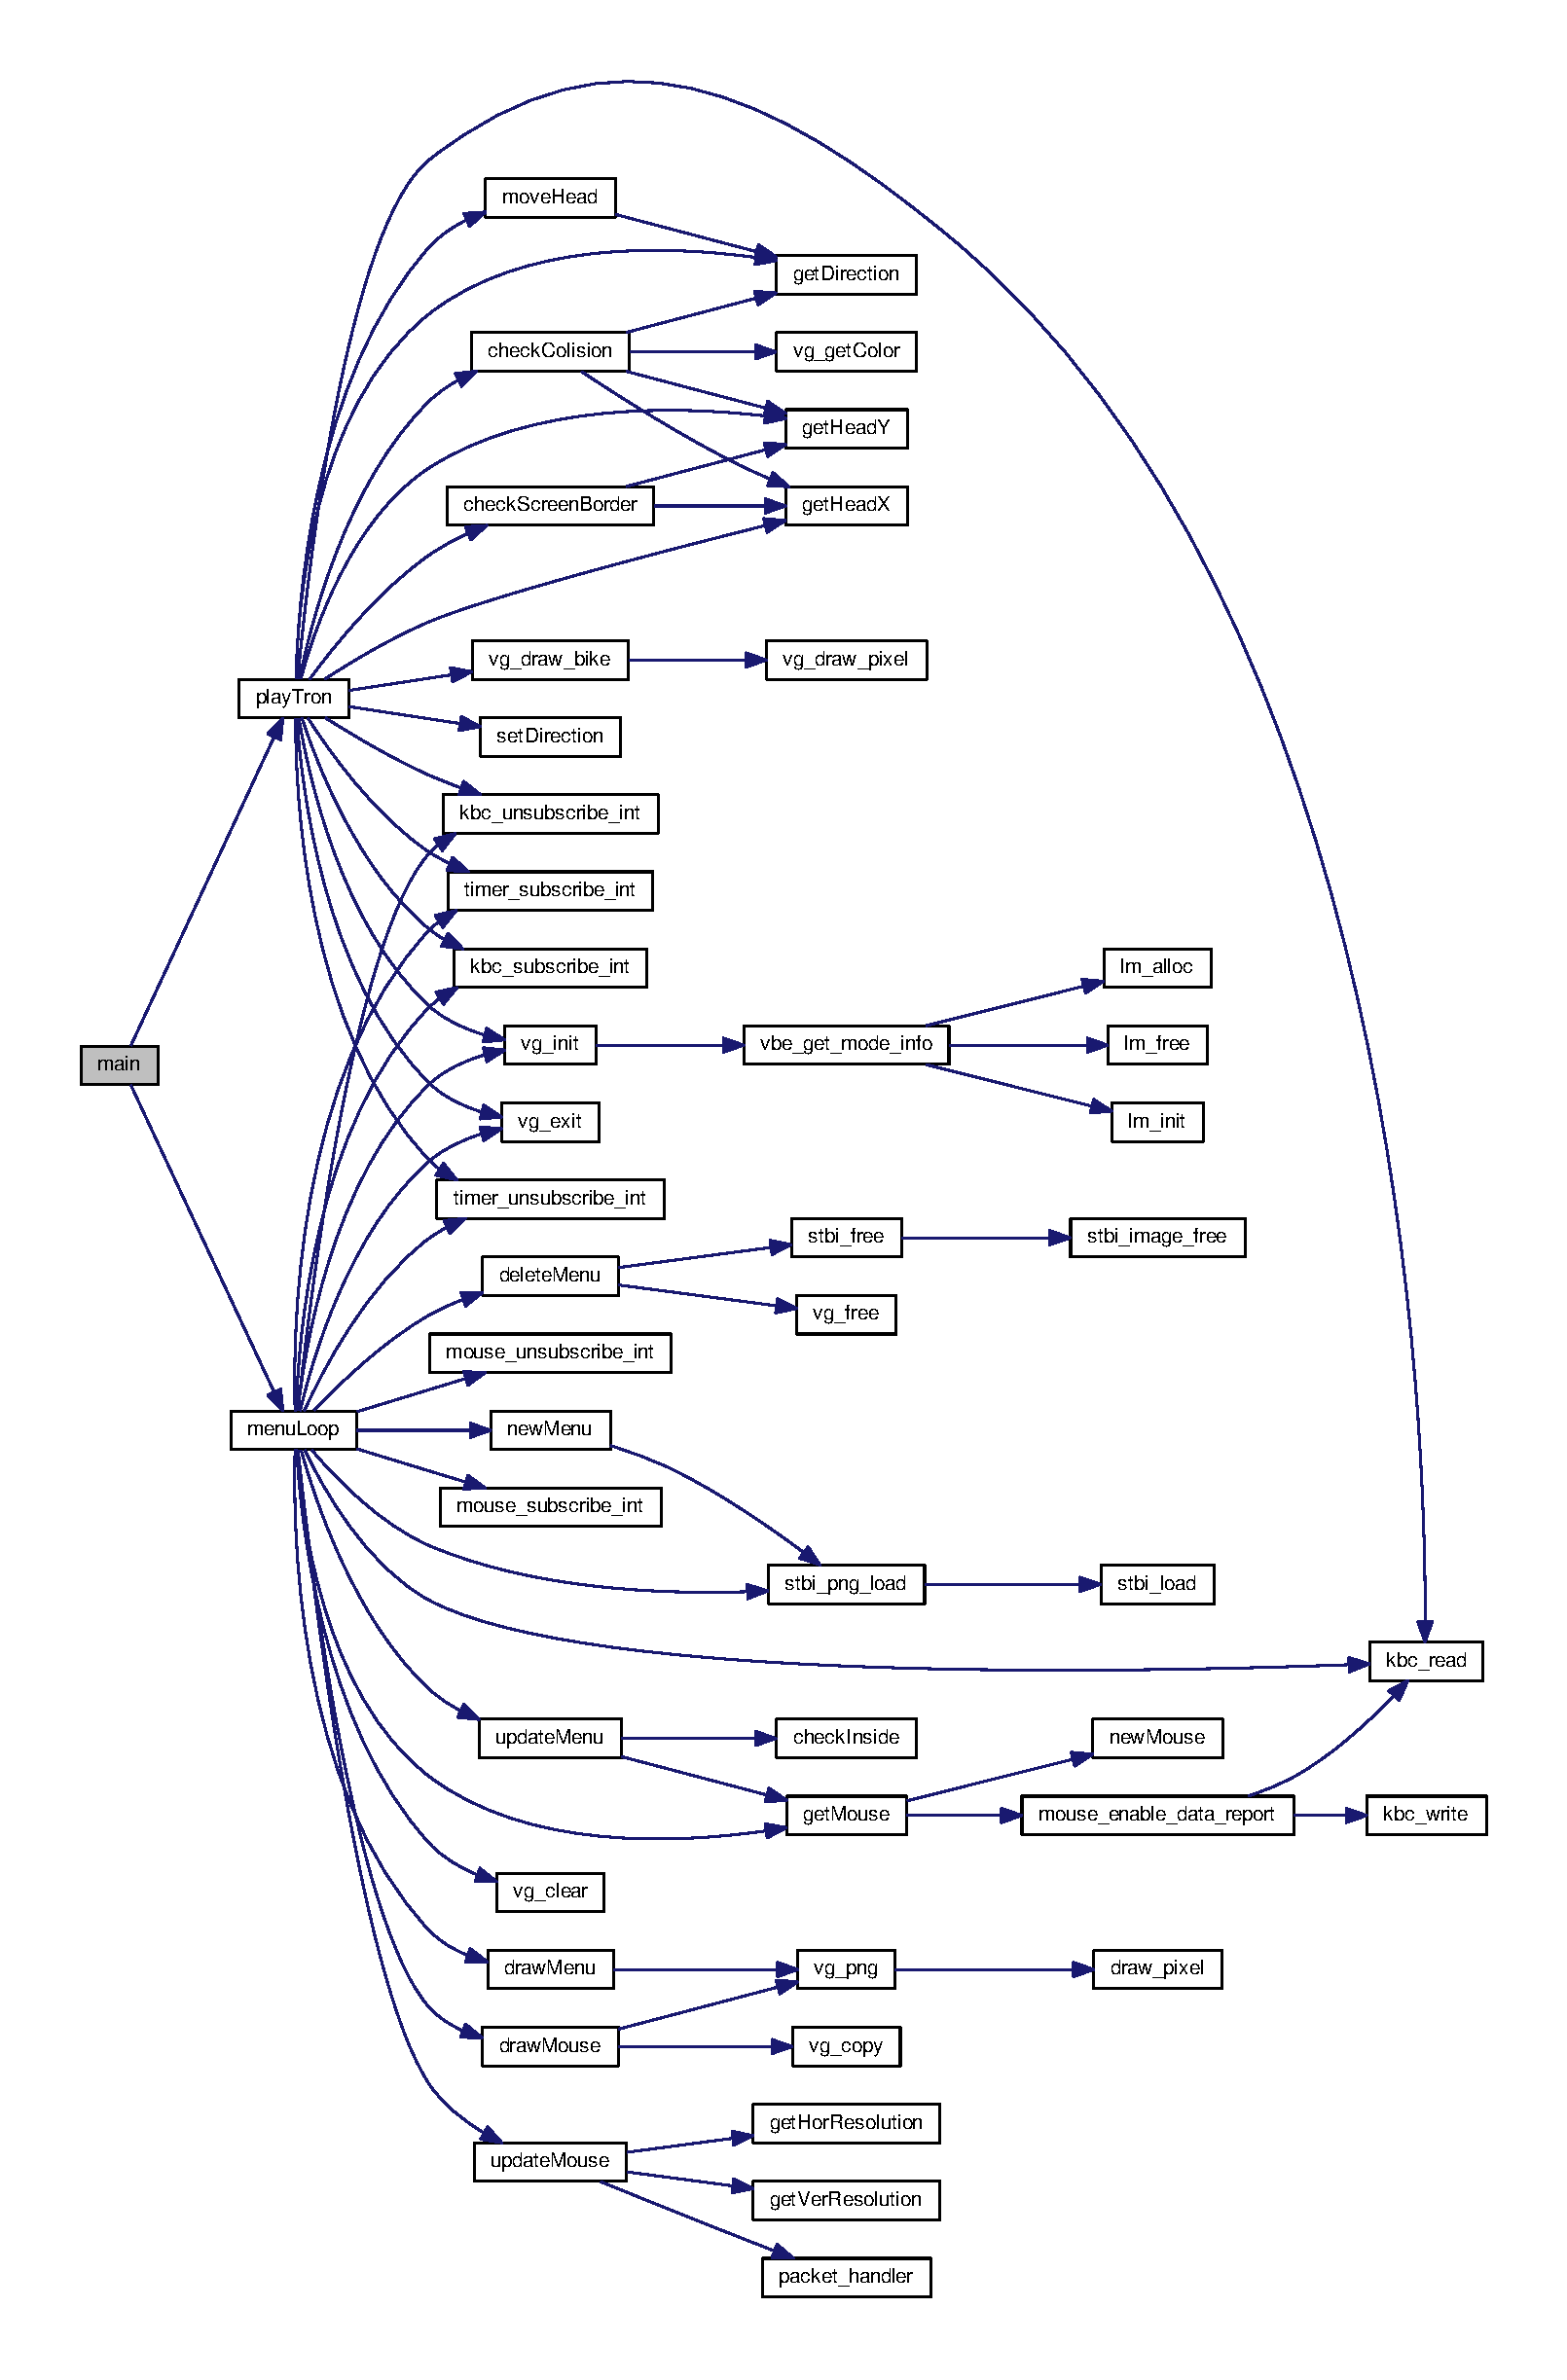
\includegraphics[width=350pt]{main_8c_ae66f6b31b5ad750f1fe042a706a4e3d4_cgraph}
\end{center}
\end{figure}



\hypertarget{mainMenu_8c}{}\section{main\+Menu.\+c File Reference}
\label{mainMenu_8c}\index{main\+Menu.\+c@{main\+Menu.\+c}}
{\ttfamily \#include $<$minix/drivers.\+h$>$}\\*
{\ttfamily \#include $<$minix/syslib.\+h$>$}\\*
{\ttfamily \#include $<$minix/driver.\+h$>$}\\*
{\ttfamily \#include $<$minix/com.\+h$>$}\\*
{\ttfamily \#include $<$minix/sysutil.\+h$>$}\\*
{\ttfamily \#include $<$limits.\+h$>$}\\*
{\ttfamily \#include $<$string.\+h$>$}\\*
{\ttfamily \#include $<$errno.\+h$>$}\\*
{\ttfamily \#include $<$stdio.\+h$>$}\\*
{\ttfamily \#include $<$math.\+h$>$}\\*
{\ttfamily \#include \char`\"{}video\+\_\+gr.\+h\char`\"{}}\\*
{\ttfamily \#include \char`\"{}keyboard.\+h\char`\"{}}\\*
{\ttfamily \#include \char`\"{}mouse.\+h\char`\"{}}\\*
{\ttfamily \#include \char`\"{}i8042.\+h\char`\"{}}\\*
{\ttfamily \#include \char`\"{}timer.\+h\char`\"{}}\\*
{\ttfamily \#include \char`\"{}i8254.\+h\char`\"{}}\\*
{\ttfamily \#include \char`\"{}menu.\+h\char`\"{}}\\*
{\ttfamily \#include \char`\"{}stbi\+\_\+wrapper.\+h\char`\"{}}\\*
Include dependency graph for main\+Menu.\+c\+:
\nopagebreak
\begin{figure}[H]
\begin{center}
\leavevmode
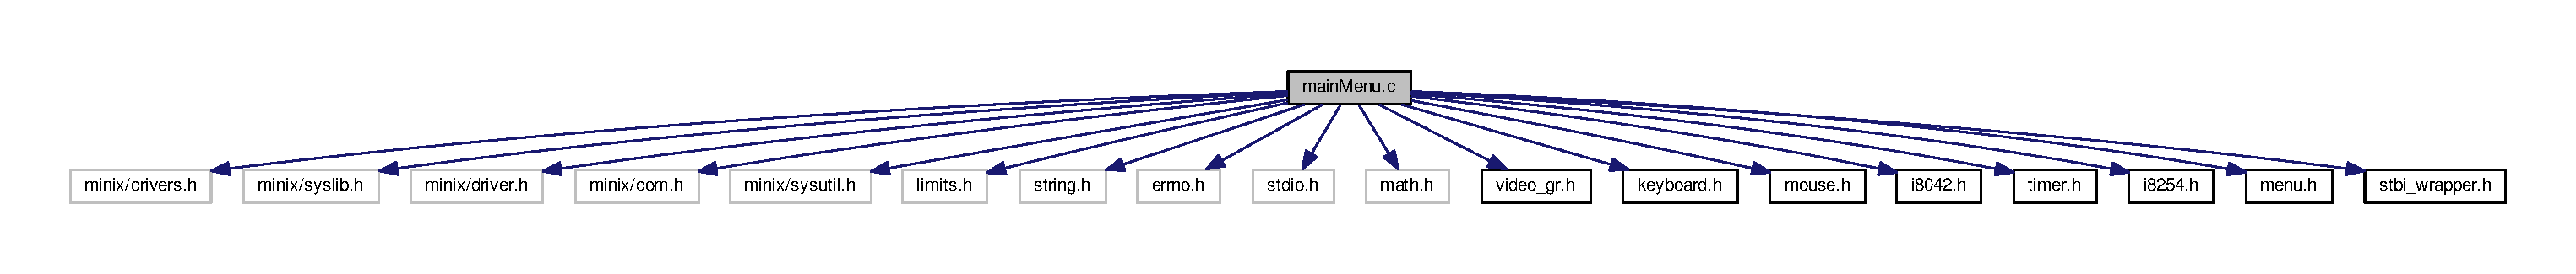
\includegraphics[width=350pt]{mainMenu_8c__incl}
\end{center}
\end{figure}
\subsection*{Functions}
\begin{DoxyCompactItemize}
\item 
int \hyperlink{mainMenu_8c_a56b618e5c9421e5ff7b20dd5c8733648}{menu\+Loop} ()
\begin{DoxyCompactList}\small\item\em menu loop \end{DoxyCompactList}\end{DoxyCompactItemize}


\subsection{Function Documentation}
\index{main\+Menu.\+c@{main\+Menu.\+c}!menu\+Loop@{menu\+Loop}}
\index{menu\+Loop@{menu\+Loop}!main\+Menu.\+c@{main\+Menu.\+c}}
\subsubsection[{\texorpdfstring{menu\+Loop()}{menuLoop()}}]{\setlength{\rightskip}{0pt plus 5cm}int menu\+Loop (
\begin{DoxyParamCaption}
{}
\end{DoxyParamCaption}
)}\hypertarget{mainMenu_8c_a56b618e5c9421e5ff7b20dd5c8733648}{}\label{mainMenu_8c_a56b618e5c9421e5ff7b20dd5c8733648}


menu loop 

\begin{DoxyReturn}{Returns}
0 if success, 1 otherwise 
\end{DoxyReturn}


Here is the call graph for this function\+:
\nopagebreak
\begin{figure}[H]
\begin{center}
\leavevmode
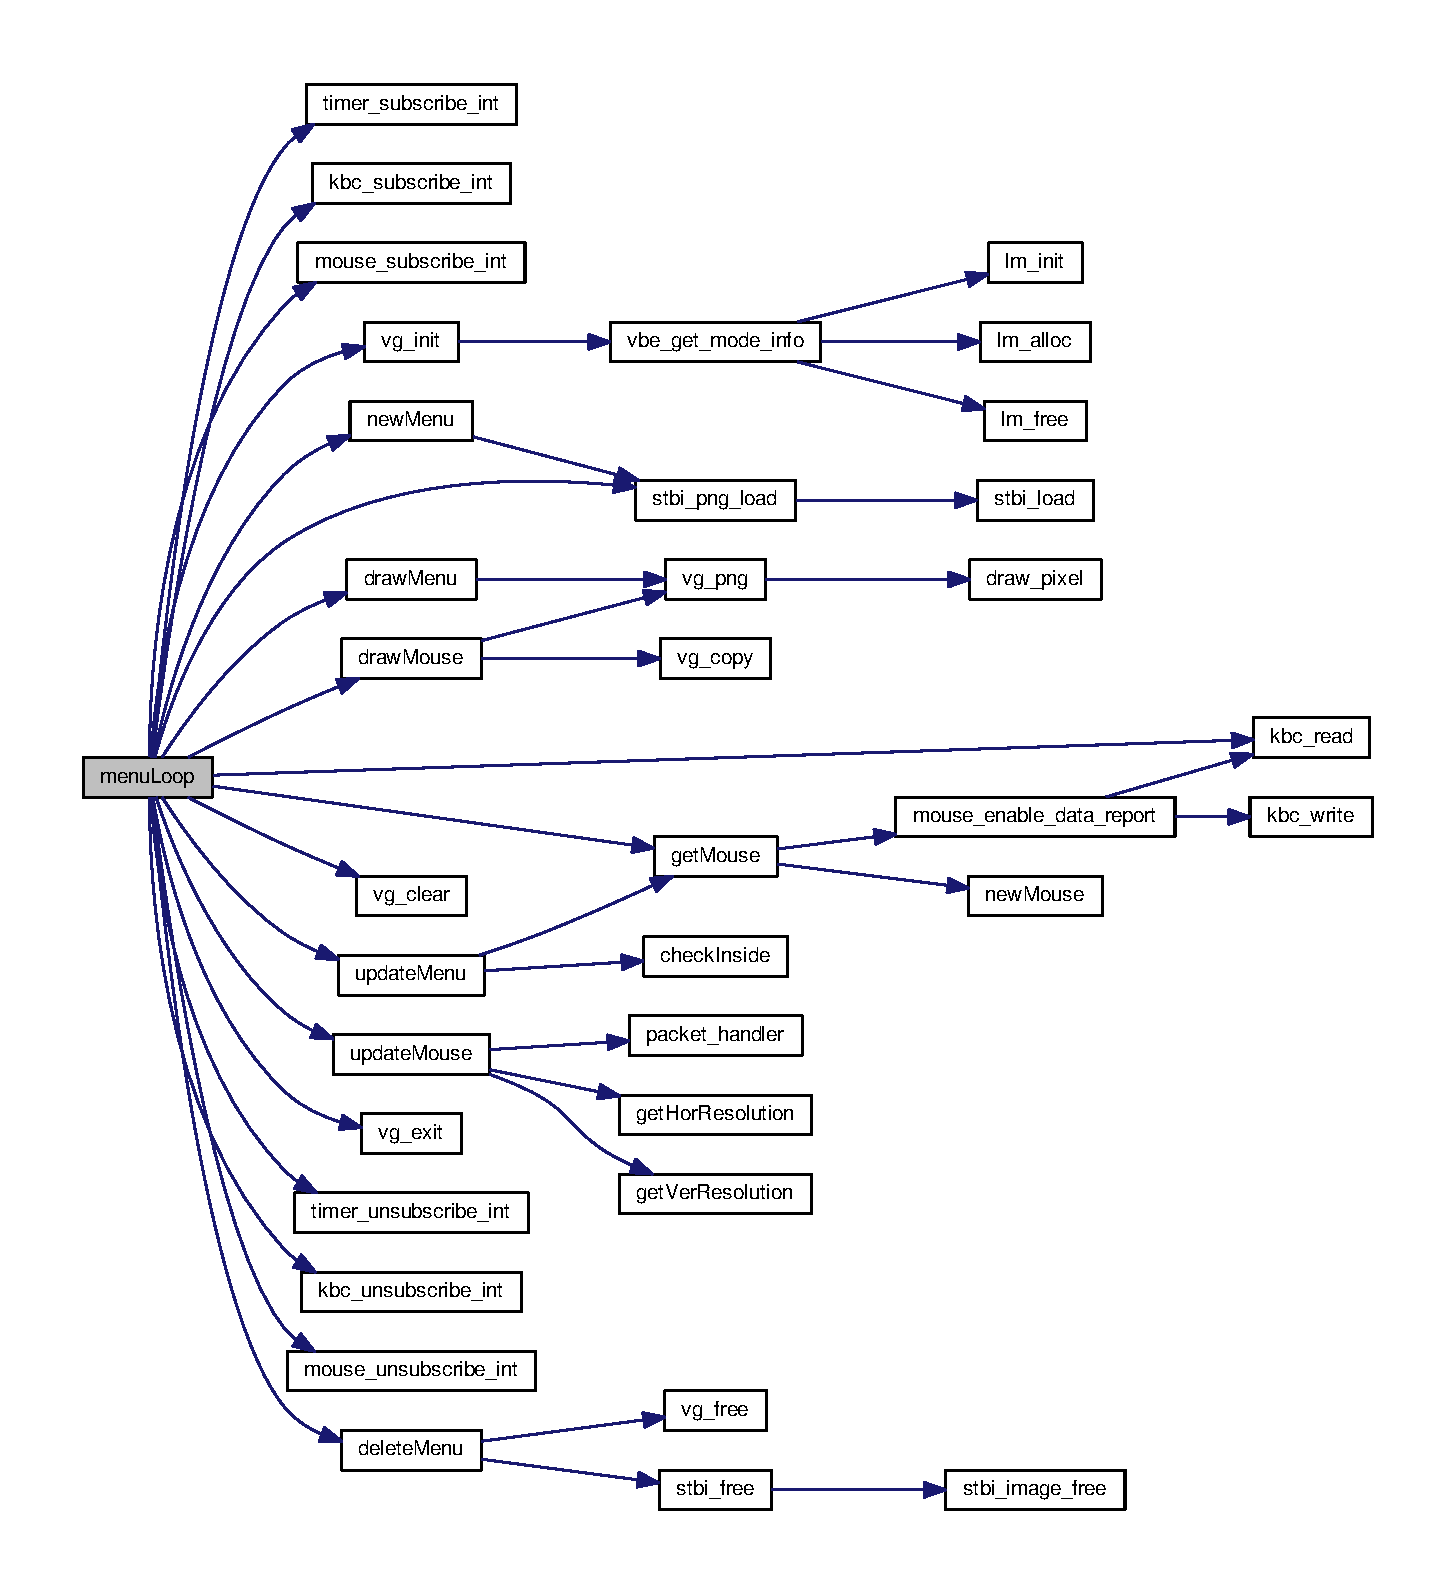
\includegraphics[width=350pt]{mainMenu_8c_a56b618e5c9421e5ff7b20dd5c8733648_cgraph}
\end{center}
\end{figure}



\hypertarget{mainMenu_8h}{}\section{main\+Menu.\+h File Reference}
\label{mainMenu_8h}\index{main\+Menu.\+h@{main\+Menu.\+h}}
This graph shows which files directly or indirectly include this file\+:
\nopagebreak
\begin{figure}[H]
\begin{center}
\leavevmode
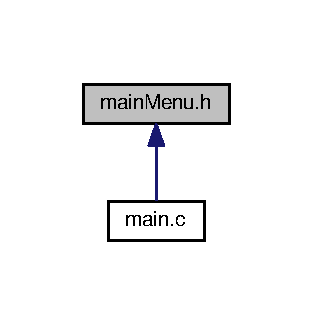
\includegraphics[width=150pt]{mainMenu_8h__dep__incl}
\end{center}
\end{figure}
\subsection*{Functions}
\begin{DoxyCompactItemize}
\item 
int \hyperlink{mainMenu_8h_a56b618e5c9421e5ff7b20dd5c8733648}{menu\+Loop} ()
\begin{DoxyCompactList}\small\item\em menu loop \end{DoxyCompactList}\end{DoxyCompactItemize}


\subsection{Function Documentation}
\index{main\+Menu.\+h@{main\+Menu.\+h}!menu\+Loop@{menu\+Loop}}
\index{menu\+Loop@{menu\+Loop}!main\+Menu.\+h@{main\+Menu.\+h}}
\subsubsection[{\texorpdfstring{menu\+Loop()}{menuLoop()}}]{\setlength{\rightskip}{0pt plus 5cm}int menu\+Loop (
\begin{DoxyParamCaption}
{}
\end{DoxyParamCaption}
)}\hypertarget{mainMenu_8h_a56b618e5c9421e5ff7b20dd5c8733648}{}\label{mainMenu_8h_a56b618e5c9421e5ff7b20dd5c8733648}


menu loop 

\begin{DoxyReturn}{Returns}
0 if success, 1 otherwise 
\end{DoxyReturn}


Here is the call graph for this function\+:
\nopagebreak
\begin{figure}[H]
\begin{center}
\leavevmode
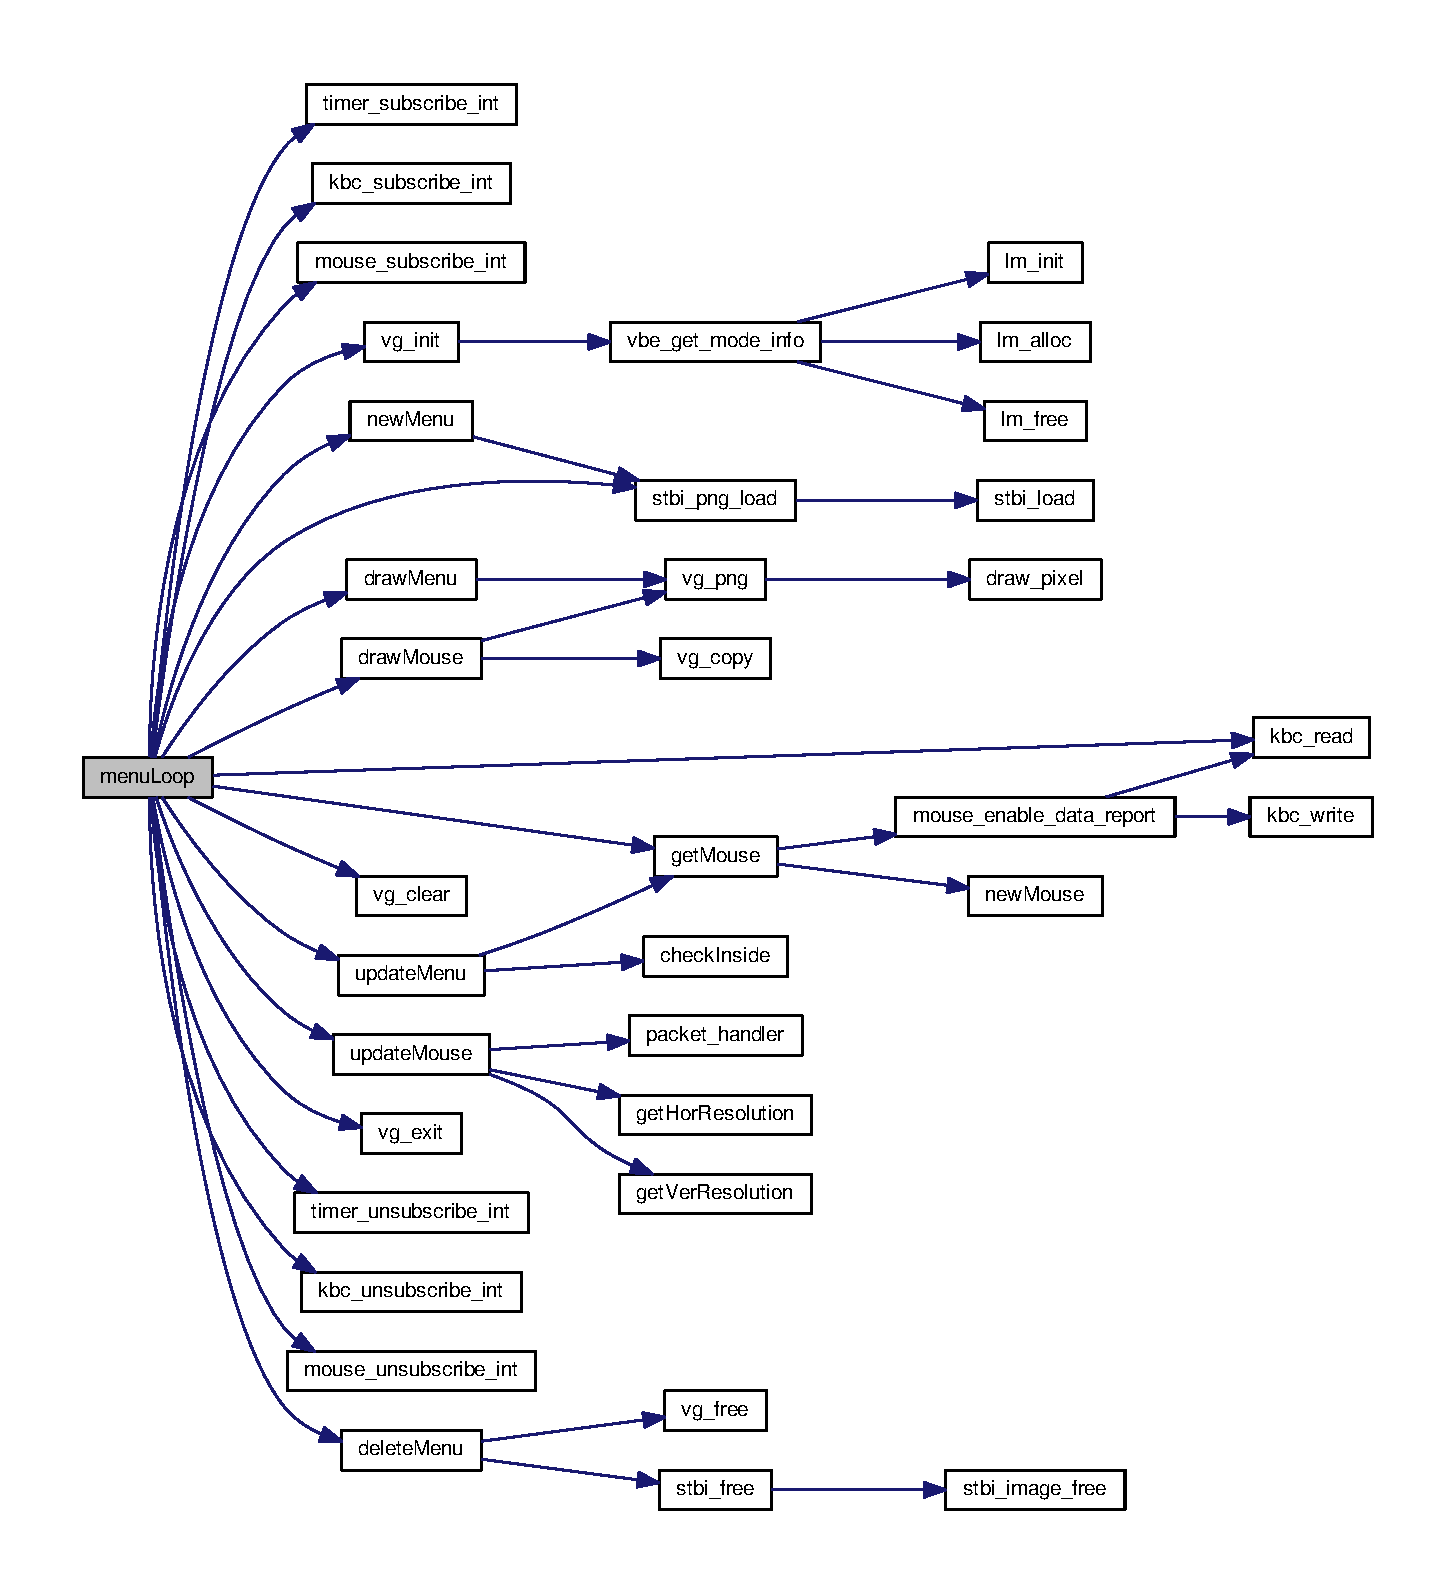
\includegraphics[width=350pt]{mainMenu_8h_a56b618e5c9421e5ff7b20dd5c8733648_cgraph}
\end{center}
\end{figure}



\hypertarget{menu_8c}{}\section{menu.\+c File Reference}
\label{menu_8c}\index{menu.\+c@{menu.\+c}}
{\ttfamily \#include $<$stdlib.\+h$>$}\\*
{\ttfamily \#include \char`\"{}menu.\+h\char`\"{}}\\*
{\ttfamily \#include \char`\"{}video\+\_\+gr.\+h\char`\"{}}\\*
{\ttfamily \#include \char`\"{}mouse.\+h\char`\"{}}\\*
{\ttfamily \#include \char`\"{}i8042.\+h\char`\"{}}\\*
{\ttfamily \#include \char`\"{}stbi\+\_\+wrapper.\+h\char`\"{}}\\*
Include dependency graph for menu.\+c\+:
\nopagebreak
\begin{figure}[H]
\begin{center}
\leavevmode
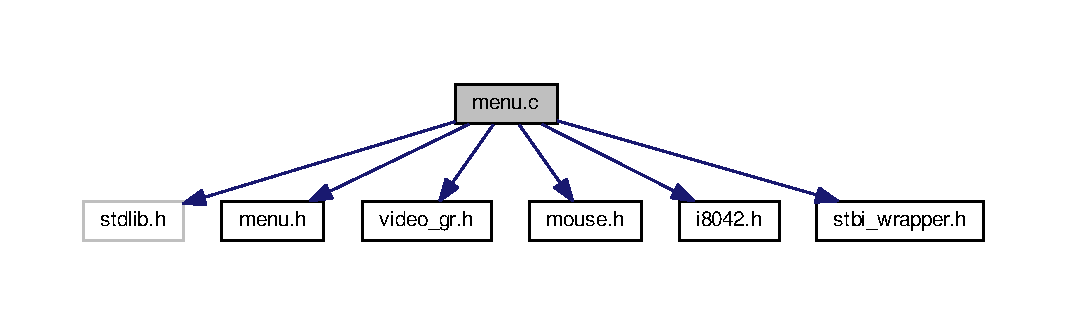
\includegraphics[width=350pt]{menu_8c__incl}
\end{center}
\end{figure}
\subsection*{Functions}
\begin{DoxyCompactItemize}
\item 
\hyperlink{structMenu}{Menu} $\ast$ \hyperlink{group__Menu_gab4c4331657aad73fe461b1946d6a80e6}{new\+Menu} ()
\begin{DoxyCompactList}\small\item\em creates a new \hyperlink{structMenu}{Menu} instance \end{DoxyCompactList}\item 
void \hyperlink{group__Menu_gab3392fb7e40877fd1ea754606fc9f8a1}{update\+Menu} (\hyperlink{structMenu}{Menu} $\ast$state, unsigned long scan\+\_\+code)
\begin{DoxyCompactList}\small\item\em updates the \hyperlink{structMenu}{Menu} \end{DoxyCompactList}\item 
void \hyperlink{group__Menu_gaf953dd83cbfca767233cb1c5f78eb266}{draw\+Menu} (\hyperlink{structMenu}{Menu} $\ast$state)
\begin{DoxyCompactList}\small\item\em draws \hyperlink{structMenu}{Menu} \end{DoxyCompactList}\item 
void \hyperlink{group__Menu_gaf155dd05949566ff9a0f29d8759bcd54}{delete\+Menu} (\hyperlink{structMenu}{Menu} $\ast$state)
\begin{DoxyCompactList}\small\item\em deletes \hyperlink{structMenu}{Menu} \end{DoxyCompactList}\end{DoxyCompactItemize}
\subsection*{Variables}
\begin{DoxyCompactItemize}
\item 
int \hyperlink{menu_8c_ac3897a350075920efc6bab8d04cc1215}{winner} = 0
\end{DoxyCompactItemize}


\subsection{Variable Documentation}
\index{menu.\+c@{menu.\+c}!winner@{winner}}
\index{winner@{winner}!menu.\+c@{menu.\+c}}
\subsubsection[{\texorpdfstring{winner}{winner}}]{\setlength{\rightskip}{0pt plus 5cm}int winner = 0}\hypertarget{menu_8c_ac3897a350075920efc6bab8d04cc1215}{}\label{menu_8c_ac3897a350075920efc6bab8d04cc1215}

\hypertarget{menu_8h}{}\section{menu.\+h File Reference}
\label{menu_8h}\index{menu.\+h@{menu.\+h}}
This graph shows which files directly or indirectly include this file\+:
\nopagebreak
\begin{figure}[H]
\begin{center}
\leavevmode
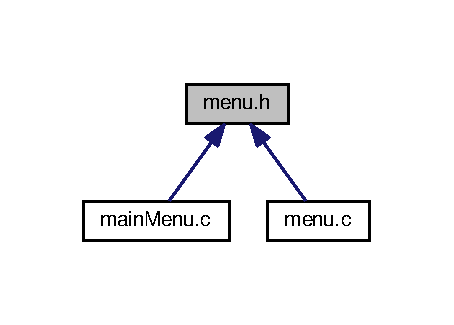
\includegraphics[width=218pt]{menu_8h__dep__incl}
\end{center}
\end{figure}
\subsection*{Classes}
\begin{DoxyCompactItemize}
\item 
struct \hyperlink{structMenu}{Menu}
\end{DoxyCompactItemize}
\subsection*{Enumerations}
\begin{DoxyCompactItemize}
\item 
enum \hyperlink{group__Menu_gab99074a1f6b7e8ff7730342913aae3a3}{Menu\+Action} \{ \hyperlink{group__Menu_ggab99074a1f6b7e8ff7730342913aae3a3a4bf4cbde18067e0600c7c8a7a30ba316}{E\+X\+I\+T\+\_\+\+G\+A\+ME}, 
\hyperlink{group__Menu_ggab99074a1f6b7e8ff7730342913aae3a3ac258a51e9cc26e302562d2bd792430b1}{P\+L\+A\+Y\+\_\+\+G\+A\+ME}
 \}
\end{DoxyCompactItemize}
\subsection*{Functions}
\begin{DoxyCompactItemize}
\item 
\hyperlink{structMenu}{Menu} $\ast$ \hyperlink{group__Menu_gab4c4331657aad73fe461b1946d6a80e6}{new\+Menu} ()
\begin{DoxyCompactList}\small\item\em creates a new \hyperlink{structMenu}{Menu} instance \end{DoxyCompactList}\item 
void \hyperlink{group__Menu_gab3392fb7e40877fd1ea754606fc9f8a1}{update\+Menu} (\hyperlink{structMenu}{Menu} $\ast$state, unsigned long scan\+\_\+code)
\begin{DoxyCompactList}\small\item\em updates the \hyperlink{structMenu}{Menu} \end{DoxyCompactList}\item 
void \hyperlink{group__Menu_gaf953dd83cbfca767233cb1c5f78eb266}{draw\+Menu} (\hyperlink{structMenu}{Menu} $\ast$state)
\begin{DoxyCompactList}\small\item\em draws \hyperlink{structMenu}{Menu} \end{DoxyCompactList}\item 
void \hyperlink{group__Menu_gaf155dd05949566ff9a0f29d8759bcd54}{delete\+Menu} (\hyperlink{structMenu}{Menu} $\ast$state)
\begin{DoxyCompactList}\small\item\em deletes \hyperlink{structMenu}{Menu} \end{DoxyCompactList}\end{DoxyCompactItemize}

\hypertarget{mouse_8c}{}\section{mouse.\+c File Reference}
\label{mouse_8c}\index{mouse.\+c@{mouse.\+c}}
{\ttfamily \#include $<$minix/syslib.\+h$>$}\\*
{\ttfamily \#include $<$minix/drivers.\+h$>$}\\*
{\ttfamily \#include $<$minix/driver.\+h$>$}\\*
{\ttfamily \#include $<$minix/com.\+h$>$}\\*
{\ttfamily \#include $<$minix/sysutil.\+h$>$}\\*
{\ttfamily \#include \char`\"{}mouse.\+h\char`\"{}}\\*
{\ttfamily \#include \char`\"{}i8042.\+h\char`\"{}}\\*
{\ttfamily \#include \char`\"{}keyboard.\+h\char`\"{}}\\*
{\ttfamily \#include \char`\"{}video\+\_\+gr.\+h\char`\"{}}\\*
Include dependency graph for mouse.\+c\+:
\nopagebreak
\begin{figure}[H]
\begin{center}
\leavevmode
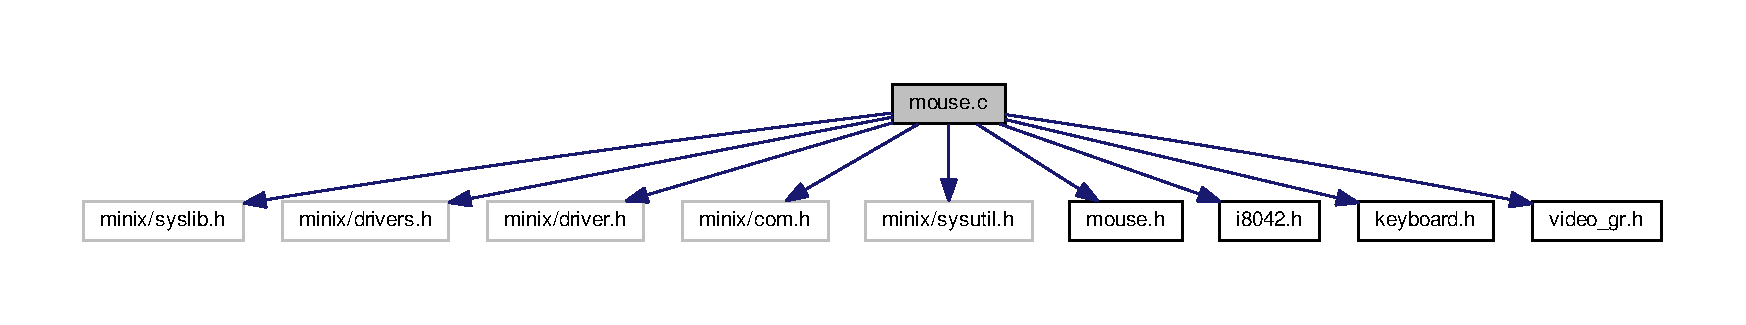
\includegraphics[width=350pt]{mouse_8c__incl}
\end{center}
\end{figure}
\subsection*{Functions}
\begin{DoxyCompactItemize}
\item 
\hyperlink{structMouse}{Mouse} $\ast$ \hyperlink{group__Mouse_gabd64fd476265e0fb0463cc3d82823701}{new\+Mouse} ()
\begin{DoxyCompactList}\small\item\em new mouse instantiation \end{DoxyCompactList}\item 
\hyperlink{structMouse}{Mouse} $\ast$ \hyperlink{group__Mouse_ga8d3f3987b96a716cc9c3aa8e484ff1d7}{get\+Mouse} ()
\begin{DoxyCompactList}\small\item\em gets the mouse object \end{DoxyCompactList}\item 
void \hyperlink{group__Mouse_ga6498182307b6c3f4a9c9c03a9d5116dc}{update\+Mouse} ()
\item 
int \hyperlink{group__Mouse_ga5075265654e56158f16cdbb0f0e4e94b}{check\+Inside} (unsigned xi, unsigned xf, unsigned yi, unsigned yf)
\begin{DoxyCompactList}\small\item\em check if the mouse is inside the window \end{DoxyCompactList}\item 
void \hyperlink{group__Mouse_ga6a0f0fbd9fee2962ff384838bbf9fade}{draw\+Mouse} (unsigned char $\ast$cursor, int width, int height)
\begin{DoxyCompactList}\small\item\em new mouse instantiation \end{DoxyCompactList}\item 
void \hyperlink{group__Mouse_ga54e27b79923964c8882407116930fc70}{delete\+Mouse} ()
\item 
void \hyperlink{group__Mouse_ga44baaa1c128be31e1baba247c3b4b6db}{packet\+\_\+handler} ()
\item 
int \hyperlink{group__Mouse_ga51e6ee02a5c0a7e618abde7250cd0841}{mouse\+\_\+subscribe\+\_\+int} (void)
\begin{DoxyCompactList}\small\item\em Subscribes and enables K\+BC interrupts. \end{DoxyCompactList}\item 
int \hyperlink{group__Mouse_ga685ad2706aca36d9869a30a19b9f446a}{mouse\+\_\+unsubscribe\+\_\+int} ()
\begin{DoxyCompactList}\small\item\em Unsubscribes K\+BC interrupts. \end{DoxyCompactList}\item 
int \hyperlink{group__Mouse_ga108813d01ba189cc8bb0dca728c932a8}{mouse\+\_\+enable\+\_\+data\+\_\+report} ()
\begin{DoxyCompactList}\small\item\em Enable mouse data report in stream mode. \end{DoxyCompactList}\item 
int \hyperlink{group__Mouse_gac13ad81d843b4d50815de4b20a28db53}{mouse\+\_\+disable\+\_\+data\+\_\+report} ()
\begin{DoxyCompactList}\small\item\em Disable mouse data report in stream mode. \end{DoxyCompactList}\item 
int \hyperlink{group__Mouse_ga16a521d1919cbd8f434d8b5d535a639b}{mouse\+\_\+set\+\_\+stream\+\_\+mode} ()
\begin{DoxyCompactList}\small\item\em Puts mouse working in stream mode. \end{DoxyCompactList}\item 
int \hyperlink{group__Mouse_ga1e54e352956b51fbf324d36d24befcbb}{mouse\+\_\+get\+\_\+packet} ()
\begin{DoxyCompactList}\small\item\em Gets the mouse packets and prints them on the screen. \end{DoxyCompactList}\end{DoxyCompactItemize}
\subsection*{Variables}
\begin{DoxyCompactItemize}
\item 
static int \hyperlink{mouse_8c_a655114c5597909d686fafff730800fd5}{mouse\+\_\+hook} = 2
\item 
unsigned char \hyperlink{mouse_8c_a1d1878244696a8be772aa71772c33f0a}{packet} \mbox{[}3\mbox{]} =\char`\"{}\char`\"{}
\item 
int \hyperlink{mouse_8c_af3d48a184a309cb0e6f6f129f2b100a5}{sync\+\_\+flag} = 0
\item 
int \hyperlink{mouse_8c_a87bfc583bc37bf9b820d7fdd9a08e43f}{packet\+\_\+index} = 0
\item 
unsigned long \hyperlink{mouse_8c_ad336f99e60a6f3d22101ca8ca6f27203}{byte}
\item 
\hyperlink{structMouse}{Mouse} $\ast$ \hyperlink{mouse_8c_a2514b83cbae6998a57eae74a24f6faf4}{mouse} = N\+U\+LL
\end{DoxyCompactItemize}


\subsection{Variable Documentation}
\index{mouse.\+c@{mouse.\+c}!byte@{byte}}
\index{byte@{byte}!mouse.\+c@{mouse.\+c}}
\subsubsection[{\texorpdfstring{byte}{byte}}]{\setlength{\rightskip}{0pt plus 5cm}unsigned long byte}\hypertarget{mouse_8c_ad336f99e60a6f3d22101ca8ca6f27203}{}\label{mouse_8c_ad336f99e60a6f3d22101ca8ca6f27203}
\index{mouse.\+c@{mouse.\+c}!mouse@{mouse}}
\index{mouse@{mouse}!mouse.\+c@{mouse.\+c}}
\subsubsection[{\texorpdfstring{mouse}{mouse}}]{\setlength{\rightskip}{0pt plus 5cm}{\bf Mouse}$\ast$ mouse = N\+U\+LL}\hypertarget{mouse_8c_a2514b83cbae6998a57eae74a24f6faf4}{}\label{mouse_8c_a2514b83cbae6998a57eae74a24f6faf4}
\index{mouse.\+c@{mouse.\+c}!mouse\+\_\+hook@{mouse\+\_\+hook}}
\index{mouse\+\_\+hook@{mouse\+\_\+hook}!mouse.\+c@{mouse.\+c}}
\subsubsection[{\texorpdfstring{mouse\+\_\+hook}{mouse_hook}}]{\setlength{\rightskip}{0pt plus 5cm}int mouse\+\_\+hook = 2\hspace{0.3cm}{\ttfamily [static]}}\hypertarget{mouse_8c_a655114c5597909d686fafff730800fd5}{}\label{mouse_8c_a655114c5597909d686fafff730800fd5}
\index{mouse.\+c@{mouse.\+c}!packet@{packet}}
\index{packet@{packet}!mouse.\+c@{mouse.\+c}}
\subsubsection[{\texorpdfstring{packet}{packet}}]{\setlength{\rightskip}{0pt plus 5cm}unsigned char packet\mbox{[}3\mbox{]} =\char`\"{}\char`\"{}}\hypertarget{mouse_8c_a1d1878244696a8be772aa71772c33f0a}{}\label{mouse_8c_a1d1878244696a8be772aa71772c33f0a}
\index{mouse.\+c@{mouse.\+c}!packet\+\_\+index@{packet\+\_\+index}}
\index{packet\+\_\+index@{packet\+\_\+index}!mouse.\+c@{mouse.\+c}}
\subsubsection[{\texorpdfstring{packet\+\_\+index}{packet_index}}]{\setlength{\rightskip}{0pt plus 5cm}int packet\+\_\+index = 0}\hypertarget{mouse_8c_a87bfc583bc37bf9b820d7fdd9a08e43f}{}\label{mouse_8c_a87bfc583bc37bf9b820d7fdd9a08e43f}
\index{mouse.\+c@{mouse.\+c}!sync\+\_\+flag@{sync\+\_\+flag}}
\index{sync\+\_\+flag@{sync\+\_\+flag}!mouse.\+c@{mouse.\+c}}
\subsubsection[{\texorpdfstring{sync\+\_\+flag}{sync_flag}}]{\setlength{\rightskip}{0pt plus 5cm}int sync\+\_\+flag = 0}\hypertarget{mouse_8c_af3d48a184a309cb0e6f6f129f2b100a5}{}\label{mouse_8c_af3d48a184a309cb0e6f6f129f2b100a5}

\hypertarget{mouse_8h}{}\section{mouse.\+h File Reference}
\label{mouse_8h}\index{mouse.\+h@{mouse.\+h}}
This graph shows which files directly or indirectly include this file\+:
\nopagebreak
\begin{figure}[H]
\begin{center}
\leavevmode
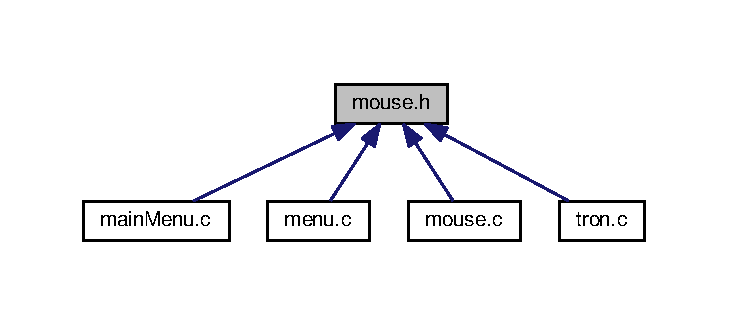
\includegraphics[width=350pt]{mouse_8h__dep__incl}
\end{center}
\end{figure}
\subsection*{Classes}
\begin{DoxyCompactItemize}
\item 
struct \hyperlink{structMouse}{Mouse}
\end{DoxyCompactItemize}
\subsection*{Functions}
\begin{DoxyCompactItemize}
\item 
\hyperlink{structMouse}{Mouse} $\ast$ \hyperlink{group__Mouse_gabd64fd476265e0fb0463cc3d82823701}{new\+Mouse} ()
\begin{DoxyCompactList}\small\item\em new mouse instantiation \end{DoxyCompactList}\item 
\hyperlink{structMouse}{Mouse} $\ast$ \hyperlink{group__Mouse_ga8d3f3987b96a716cc9c3aa8e484ff1d7}{get\+Mouse} ()
\begin{DoxyCompactList}\small\item\em gets the mouse object \end{DoxyCompactList}\item 
void \hyperlink{group__Mouse_ga6498182307b6c3f4a9c9c03a9d5116dc}{update\+Mouse} ()
\item 
void \hyperlink{group__Mouse_ga6a0f0fbd9fee2962ff384838bbf9fade}{draw\+Mouse} (unsigned char $\ast$cursor, int width, int height)
\begin{DoxyCompactList}\small\item\em new mouse instantiation \end{DoxyCompactList}\item 
void \hyperlink{group__Mouse_ga54e27b79923964c8882407116930fc70}{delete\+Mouse} ()
\item 
void \hyperlink{group__Mouse_ga44baaa1c128be31e1baba247c3b4b6db}{packet\+\_\+handler} ()
\item 
int \hyperlink{group__Mouse_ga5075265654e56158f16cdbb0f0e4e94b}{check\+Inside} (unsigned xi, unsigned xf, unsigned yi, unsigned yf)
\begin{DoxyCompactList}\small\item\em check if the mouse is inside the window \end{DoxyCompactList}\item 
int \hyperlink{group__Mouse_ga51e6ee02a5c0a7e618abde7250cd0841}{mouse\+\_\+subscribe\+\_\+int} (void)
\begin{DoxyCompactList}\small\item\em Subscribes and enables K\+BC interrupts. \end{DoxyCompactList}\item 
int \hyperlink{group__Mouse_ga685ad2706aca36d9869a30a19b9f446a}{mouse\+\_\+unsubscribe\+\_\+int} ()
\begin{DoxyCompactList}\small\item\em Unsubscribes K\+BC interrupts. \end{DoxyCompactList}\item 
int \hyperlink{group__Mouse_ga108813d01ba189cc8bb0dca728c932a8}{mouse\+\_\+enable\+\_\+data\+\_\+report} ()
\begin{DoxyCompactList}\small\item\em Enable mouse data report in stream mode. \end{DoxyCompactList}\item 
int \hyperlink{group__Mouse_gac13ad81d843b4d50815de4b20a28db53}{mouse\+\_\+disable\+\_\+data\+\_\+report} ()
\begin{DoxyCompactList}\small\item\em Disable mouse data report in stream mode. \end{DoxyCompactList}\item 
int \hyperlink{group__Mouse_ga16a521d1919cbd8f434d8b5d535a639b}{mouse\+\_\+set\+\_\+stream\+\_\+mode} ()
\begin{DoxyCompactList}\small\item\em Puts mouse working in stream mode. \end{DoxyCompactList}\item 
int \hyperlink{group__Mouse_ga1e54e352956b51fbf324d36d24befcbb}{mouse\+\_\+get\+\_\+packet} ()
\begin{DoxyCompactList}\small\item\em Gets the mouse packets and prints them on the screen. \end{DoxyCompactList}\end{DoxyCompactItemize}
\subsection*{Variables}
\begin{DoxyCompactItemize}
\item 
unsigned char \hyperlink{mouse_8h_a3db4d4abec34f9e6bf81e2ae0a48f66b}{packet} \mbox{[}$\,$\mbox{]}
\end{DoxyCompactItemize}


\subsection{Variable Documentation}
\index{mouse.\+h@{mouse.\+h}!packet@{packet}}
\index{packet@{packet}!mouse.\+h@{mouse.\+h}}
\subsubsection[{\texorpdfstring{packet}{packet}}]{\setlength{\rightskip}{0pt plus 5cm}unsigned char packet\mbox{[}$\,$\mbox{]}}\hypertarget{mouse_8h_a3db4d4abec34f9e6bf81e2ae0a48f66b}{}\label{mouse_8h_a3db4d4abec34f9e6bf81e2ae0a48f66b}

\hypertarget{stb__image_8h}{}\section{stb\+\_\+image.\+h File Reference}
\label{stb__image_8h}\index{stb\+\_\+image.\+h@{stb\+\_\+image.\+h}}
{\ttfamily \#include $<$stdio.\+h$>$}\\*
{\ttfamily \#include $<$stdarg.\+h$>$}\\*
{\ttfamily \#include $<$stddef.\+h$>$}\\*
{\ttfamily \#include $<$stdlib.\+h$>$}\\*
{\ttfamily \#include $<$string.\+h$>$}\\*
{\ttfamily \#include $<$limits.\+h$>$}\\*
{\ttfamily \#include $<$math.\+h$>$}\\*
{\ttfamily \#include $<$assert.\+h$>$}\\*
{\ttfamily \#include $<$stdint.\+h$>$}\\*
Include dependency graph for stb\+\_\+image.\+h\+:
\nopagebreak
\begin{figure}[H]
\begin{center}
\leavevmode
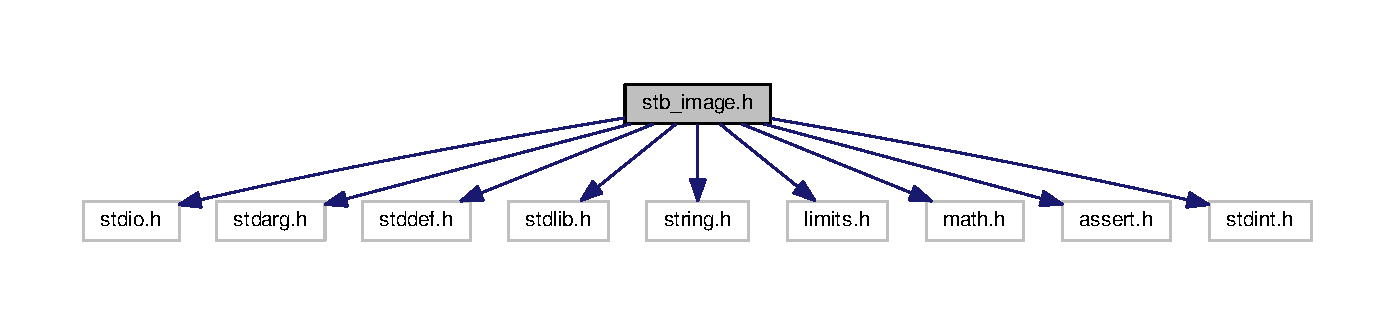
\includegraphics[width=350pt]{stb__image_8h__incl}
\end{center}
\end{figure}
This graph shows which files directly or indirectly include this file\+:
\nopagebreak
\begin{figure}[H]
\begin{center}
\leavevmode
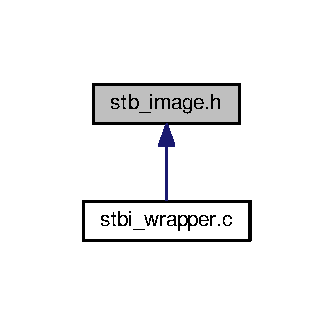
\includegraphics[width=160pt]{stb__image_8h__dep__incl}
\end{center}
\end{figure}
\subsection*{Classes}
\begin{DoxyCompactItemize}
\item 
struct \hyperlink{structstbi__io__callbacks}{stbi\+\_\+io\+\_\+callbacks}
\end{DoxyCompactItemize}
\subsection*{Macros}
\begin{DoxyCompactItemize}
\item 
\#define \hyperlink{stb__image_8h_aed6cd14a3bf678808c4c179e808866aa}{S\+T\+B\+I\+\_\+\+V\+E\+R\+S\+I\+ON}~1
\item 
\#define \hyperlink{stb__image_8h_a2d9ec9850cd12aefe7641b456266a4c2}{S\+T\+B\+I\+D\+EF}~extern
\end{DoxyCompactItemize}
\subsection*{Typedefs}
\begin{DoxyCompactItemize}
\item 
typedef unsigned char \hyperlink{stb__image_8h_a28eb51a1512ce382ee50f20e1d04d50d}{stbi\+\_\+uc}
\item 
typedef unsigned short \hyperlink{stb__image_8h_a648037d4c55689328ba08c8f5d293df2}{stbi\+\_\+us}
\end{DoxyCompactItemize}
\subsection*{Enumerations}
\begin{DoxyCompactItemize}
\item 
enum \{ \\*
\hyperlink{stb__image_8h_a06fc87d81c62e9abb8790b6e5713c55ba0177ac2c5002f4f251bb766d41752029}{S\+T\+B\+I\+\_\+default} = 0, 
\hyperlink{stb__image_8h_a06fc87d81c62e9abb8790b6e5713c55bad1eb95ca1fa7706bf732bf35a0ed40aa}{S\+T\+B\+I\+\_\+grey} = 1, 
\hyperlink{stb__image_8h_a06fc87d81c62e9abb8790b6e5713c55baf5829d16d4cca6077465c5abd346e2f8}{S\+T\+B\+I\+\_\+grey\+\_\+alpha} = 2, 
\hyperlink{stb__image_8h_a06fc87d81c62e9abb8790b6e5713c55baa59123e5d0af25f9b1539f5cf1facddf}{S\+T\+B\+I\+\_\+rgb} = 3, 
\\*
\hyperlink{stb__image_8h_a06fc87d81c62e9abb8790b6e5713c55baa7b1af0c9f0310c3ada2aa29a32de293}{S\+T\+B\+I\+\_\+rgb\+\_\+alpha} = 4
 \}
\end{DoxyCompactItemize}
\subsection*{Functions}
\begin{DoxyCompactItemize}
\item 
\hyperlink{stb__image_8h_a2d9ec9850cd12aefe7641b456266a4c2}{S\+T\+B\+I\+D\+EF} \hyperlink{stb__image_8h_a28eb51a1512ce382ee50f20e1d04d50d}{stbi\+\_\+uc} $\ast$ \hyperlink{stb__image_8h_acae25d31bfae29d75482f07fecf2935f}{stbi\+\_\+load\+\_\+from\+\_\+memory} (\hyperlink{stb__image_8h_a28eb51a1512ce382ee50f20e1d04d50d}{stbi\+\_\+uc} const $\ast$buffer, int len, int $\ast$x, int $\ast$y, int $\ast$channels\+\_\+in\+\_\+file, int desired\+\_\+channels)
\item 
\hyperlink{stb__image_8h_a2d9ec9850cd12aefe7641b456266a4c2}{S\+T\+B\+I\+D\+EF} \hyperlink{stb__image_8h_a28eb51a1512ce382ee50f20e1d04d50d}{stbi\+\_\+uc} $\ast$ \hyperlink{stb__image_8h_a95ebc5c42c1a753200be8d465e933af7}{stbi\+\_\+load\+\_\+from\+\_\+callbacks} (\hyperlink{structstbi__io__callbacks}{stbi\+\_\+io\+\_\+callbacks} const $\ast$clbk, void $\ast$user, int $\ast$x, int $\ast$y, int $\ast$channels\+\_\+in\+\_\+file, int desired\+\_\+channels)
\item 
\hyperlink{stb__image_8h_a2d9ec9850cd12aefe7641b456266a4c2}{S\+T\+B\+I\+D\+EF} \hyperlink{stb__image_8h_a28eb51a1512ce382ee50f20e1d04d50d}{stbi\+\_\+uc} $\ast$ \hyperlink{stb__image_8h_aefdc7387857a14894bbf321e9ea4f048}{stbi\+\_\+load} (char const $\ast$filename, int $\ast$x, int $\ast$y, int $\ast$channels\+\_\+in\+\_\+file, int desired\+\_\+channels)
\item 
\hyperlink{stb__image_8h_a2d9ec9850cd12aefe7641b456266a4c2}{S\+T\+B\+I\+D\+EF} \hyperlink{stb__image_8h_a28eb51a1512ce382ee50f20e1d04d50d}{stbi\+\_\+uc} $\ast$ \hyperlink{stb__image_8h_aa9994764695597161e8f3776e97caa99}{stbi\+\_\+load\+\_\+from\+\_\+file} (F\+I\+LE $\ast$f, int $\ast$x, int $\ast$y, int $\ast$channels\+\_\+in\+\_\+file, int desired\+\_\+channels)
\item 
\hyperlink{stb__image_8h_a2d9ec9850cd12aefe7641b456266a4c2}{S\+T\+B\+I\+D\+EF} \hyperlink{stb__image_8h_a648037d4c55689328ba08c8f5d293df2}{stbi\+\_\+us} $\ast$ \hyperlink{stb__image_8h_ad30fd870ed2138ce8f38c9dd29b2f76a}{stbi\+\_\+load\+\_\+16\+\_\+from\+\_\+memory} (\hyperlink{stb__image_8h_a28eb51a1512ce382ee50f20e1d04d50d}{stbi\+\_\+uc} const $\ast$buffer, int len, int $\ast$x, int $\ast$y, int $\ast$channels\+\_\+in\+\_\+file, int desired\+\_\+channels)
\item 
\hyperlink{stb__image_8h_a2d9ec9850cd12aefe7641b456266a4c2}{S\+T\+B\+I\+D\+EF} \hyperlink{stb__image_8h_a648037d4c55689328ba08c8f5d293df2}{stbi\+\_\+us} $\ast$ \hyperlink{stb__image_8h_a82bcc0957b6a4ebfdfa3d7f04fbaed18}{stbi\+\_\+load\+\_\+16\+\_\+from\+\_\+callbacks} (\hyperlink{structstbi__io__callbacks}{stbi\+\_\+io\+\_\+callbacks} const $\ast$clbk, void $\ast$user, int $\ast$x, int $\ast$y, int $\ast$channels\+\_\+in\+\_\+file, int desired\+\_\+channels)
\item 
\hyperlink{stb__image_8h_a2d9ec9850cd12aefe7641b456266a4c2}{S\+T\+B\+I\+D\+EF} \hyperlink{stb__image_8h_a648037d4c55689328ba08c8f5d293df2}{stbi\+\_\+us} $\ast$ \hyperlink{stb__image_8h_a8a58b6bcd805afa1bdb14f988dd37fee}{stbi\+\_\+load\+\_\+16} (char const $\ast$filename, int $\ast$x, int $\ast$y, int $\ast$channels\+\_\+in\+\_\+file, int desired\+\_\+channels)
\item 
\hyperlink{stb__image_8h_a2d9ec9850cd12aefe7641b456266a4c2}{S\+T\+B\+I\+D\+EF} \hyperlink{stb__image_8h_a648037d4c55689328ba08c8f5d293df2}{stbi\+\_\+us} $\ast$ \hyperlink{stb__image_8h_a9ca2591f0987284129e82bf9dbcf7c6c}{stbi\+\_\+load\+\_\+from\+\_\+file\+\_\+16} (F\+I\+LE $\ast$f, int $\ast$x, int $\ast$y, int $\ast$channels\+\_\+in\+\_\+file, int desired\+\_\+channels)
\item 
\hyperlink{stb__image_8h_a2d9ec9850cd12aefe7641b456266a4c2}{S\+T\+B\+I\+D\+EF} float $\ast$ \hyperlink{stb__image_8h_a5d47fb76ce1e34eb0729ad932c9c48e2}{stbi\+\_\+loadf\+\_\+from\+\_\+memory} (\hyperlink{stb__image_8h_a28eb51a1512ce382ee50f20e1d04d50d}{stbi\+\_\+uc} const $\ast$buffer, int len, int $\ast$x, int $\ast$y, int $\ast$channels\+\_\+in\+\_\+file, int desired\+\_\+channels)
\item 
\hyperlink{stb__image_8h_a2d9ec9850cd12aefe7641b456266a4c2}{S\+T\+B\+I\+D\+EF} float $\ast$ \hyperlink{stb__image_8h_a6e7fd261af79ecef2208df3a6cc806bb}{stbi\+\_\+loadf\+\_\+from\+\_\+callbacks} (\hyperlink{structstbi__io__callbacks}{stbi\+\_\+io\+\_\+callbacks} const $\ast$clbk, void $\ast$user, int $\ast$x, int $\ast$y, int $\ast$channels\+\_\+in\+\_\+file, int desired\+\_\+channels)
\item 
\hyperlink{stb__image_8h_a2d9ec9850cd12aefe7641b456266a4c2}{S\+T\+B\+I\+D\+EF} float $\ast$ \hyperlink{stb__image_8h_af4f17acd30945a75901fdc022f90575f}{stbi\+\_\+loadf} (char const $\ast$filename, int $\ast$x, int $\ast$y, int $\ast$channels\+\_\+in\+\_\+file, int desired\+\_\+channels)
\item 
\hyperlink{stb__image_8h_a2d9ec9850cd12aefe7641b456266a4c2}{S\+T\+B\+I\+D\+EF} float $\ast$ \hyperlink{stb__image_8h_ace82446ecd7b5c760cde062179660f46}{stbi\+\_\+loadf\+\_\+from\+\_\+file} (F\+I\+LE $\ast$f, int $\ast$x, int $\ast$y, int $\ast$channels\+\_\+in\+\_\+file, int desired\+\_\+channels)
\item 
\hyperlink{stb__image_8h_a2d9ec9850cd12aefe7641b456266a4c2}{S\+T\+B\+I\+D\+EF} void \hyperlink{stb__image_8h_ab18889e43518d6b4421b705782bb1b5e}{stbi\+\_\+hdr\+\_\+to\+\_\+ldr\+\_\+gamma} (float gamma)
\item 
\hyperlink{stb__image_8h_a2d9ec9850cd12aefe7641b456266a4c2}{S\+T\+B\+I\+D\+EF} void \hyperlink{stb__image_8h_ae21cc1184eeb5cc814699f1ed62c5258}{stbi\+\_\+hdr\+\_\+to\+\_\+ldr\+\_\+scale} (float scale)
\item 
\hyperlink{stb__image_8h_a2d9ec9850cd12aefe7641b456266a4c2}{S\+T\+B\+I\+D\+EF} void \hyperlink{stb__image_8h_a1feccdcf726dcc6b5502e3efa85b7dbb}{stbi\+\_\+ldr\+\_\+to\+\_\+hdr\+\_\+gamma} (float gamma)
\item 
\hyperlink{stb__image_8h_a2d9ec9850cd12aefe7641b456266a4c2}{S\+T\+B\+I\+D\+EF} void \hyperlink{stb__image_8h_af946583656a362a316b40c0421c20561}{stbi\+\_\+ldr\+\_\+to\+\_\+hdr\+\_\+scale} (float scale)
\item 
\hyperlink{stb__image_8h_a2d9ec9850cd12aefe7641b456266a4c2}{S\+T\+B\+I\+D\+EF} int \hyperlink{stb__image_8h_af0e94f316fe1848f632517ca3c11d077}{stbi\+\_\+is\+\_\+hdr\+\_\+from\+\_\+callbacks} (\hyperlink{structstbi__io__callbacks}{stbi\+\_\+io\+\_\+callbacks} const $\ast$clbk, void $\ast$user)
\item 
\hyperlink{stb__image_8h_a2d9ec9850cd12aefe7641b456266a4c2}{S\+T\+B\+I\+D\+EF} int \hyperlink{stb__image_8h_a5cbc6f5cbb3b2d0d87ee959fcee9d23e}{stbi\+\_\+is\+\_\+hdr\+\_\+from\+\_\+memory} (\hyperlink{stb__image_8h_a28eb51a1512ce382ee50f20e1d04d50d}{stbi\+\_\+uc} const $\ast$buffer, int len)
\item 
\hyperlink{stb__image_8h_a2d9ec9850cd12aefe7641b456266a4c2}{S\+T\+B\+I\+D\+EF} int \hyperlink{stb__image_8h_ae70f9a302f7e87fd971075e7f758d55c}{stbi\+\_\+is\+\_\+hdr} (char const $\ast$filename)
\item 
\hyperlink{stb__image_8h_a2d9ec9850cd12aefe7641b456266a4c2}{S\+T\+B\+I\+D\+EF} int \hyperlink{stb__image_8h_aaf10d41631e1e9214fde1688bdbd8524}{stbi\+\_\+is\+\_\+hdr\+\_\+from\+\_\+file} (F\+I\+LE $\ast$f)
\item 
\hyperlink{stb__image_8h_a2d9ec9850cd12aefe7641b456266a4c2}{S\+T\+B\+I\+D\+EF} const char $\ast$ \hyperlink{stb__image_8h_aa874b3ba909f3281d499894909678336}{stbi\+\_\+failure\+\_\+reason} (void)
\item 
\hyperlink{stb__image_8h_a2d9ec9850cd12aefe7641b456266a4c2}{S\+T\+B\+I\+D\+EF} void \hyperlink{stb__image_8h_ad3e11bb44412a7ba348acfbad09caacb}{stbi\+\_\+image\+\_\+free} (void $\ast$retval\+\_\+from\+\_\+stbi\+\_\+load)
\item 
\hyperlink{stb__image_8h_a2d9ec9850cd12aefe7641b456266a4c2}{S\+T\+B\+I\+D\+EF} int \hyperlink{stb__image_8h_acfef077febce3bc3f1f339de478f3315}{stbi\+\_\+info\+\_\+from\+\_\+memory} (\hyperlink{stb__image_8h_a28eb51a1512ce382ee50f20e1d04d50d}{stbi\+\_\+uc} const $\ast$buffer, int len, int $\ast$x, int $\ast$y, int $\ast$comp)
\item 
\hyperlink{stb__image_8h_a2d9ec9850cd12aefe7641b456266a4c2}{S\+T\+B\+I\+D\+EF} int \hyperlink{stb__image_8h_a86291c64cb663f41a34647d5e1abf363}{stbi\+\_\+info\+\_\+from\+\_\+callbacks} (\hyperlink{structstbi__io__callbacks}{stbi\+\_\+io\+\_\+callbacks} const $\ast$clbk, void $\ast$user, int $\ast$x, int $\ast$y, int $\ast$comp)
\item 
\hyperlink{stb__image_8h_a2d9ec9850cd12aefe7641b456266a4c2}{S\+T\+B\+I\+D\+EF} int \hyperlink{stb__image_8h_aede708cca1304520b2afcf4d5eb61d70}{stbi\+\_\+info} (char const $\ast$filename, int $\ast$x, int $\ast$y, int $\ast$comp)
\item 
\hyperlink{stb__image_8h_a2d9ec9850cd12aefe7641b456266a4c2}{S\+T\+B\+I\+D\+EF} int \hyperlink{stb__image_8h_a28abedef4a0a93909332080df6be0021}{stbi\+\_\+info\+\_\+from\+\_\+file} (F\+I\+LE $\ast$f, int $\ast$x, int $\ast$y, int $\ast$comp)
\item 
\hyperlink{stb__image_8h_a2d9ec9850cd12aefe7641b456266a4c2}{S\+T\+B\+I\+D\+EF} void \hyperlink{stb__image_8h_a3f02e0053e1c8d08a3ed436e6a82c7c9}{stbi\+\_\+set\+\_\+unpremultiply\+\_\+on\+\_\+load} (int flag\+\_\+true\+\_\+if\+\_\+should\+\_\+unpremultiply)
\item 
\hyperlink{stb__image_8h_a2d9ec9850cd12aefe7641b456266a4c2}{S\+T\+B\+I\+D\+EF} void \hyperlink{stb__image_8h_a23525ef2b882f3de426b47ecf8d9151b}{stbi\+\_\+convert\+\_\+iphone\+\_\+png\+\_\+to\+\_\+rgb} (int flag\+\_\+true\+\_\+if\+\_\+should\+\_\+convert)
\item 
\hyperlink{stb__image_8h_a2d9ec9850cd12aefe7641b456266a4c2}{S\+T\+B\+I\+D\+EF} void \hyperlink{stb__image_8h_ab89c177fc52f1bb2dc1c05e48129a0a4}{stbi\+\_\+set\+\_\+flip\+\_\+vertically\+\_\+on\+\_\+load} (int flag\+\_\+true\+\_\+if\+\_\+should\+\_\+flip)
\item 
\hyperlink{stb__image_8h_a2d9ec9850cd12aefe7641b456266a4c2}{S\+T\+B\+I\+D\+EF} char $\ast$ \hyperlink{stb__image_8h_aaaa17a529bec51403cc23dc2e7c36d79}{stbi\+\_\+zlib\+\_\+decode\+\_\+malloc\+\_\+guesssize} (const char $\ast$buffer, int len, int initial\+\_\+size, int $\ast$outlen)
\item 
\hyperlink{stb__image_8h_a2d9ec9850cd12aefe7641b456266a4c2}{S\+T\+B\+I\+D\+EF} char $\ast$ \hyperlink{stb__image_8h_a038b0e741859a482b8b9d60167e54d27}{stbi\+\_\+zlib\+\_\+decode\+\_\+malloc\+\_\+guesssize\+\_\+headerflag} (const char $\ast$buffer, int len, int initial\+\_\+size, int $\ast$outlen, int parse\+\_\+header)
\item 
\hyperlink{stb__image_8h_a2d9ec9850cd12aefe7641b456266a4c2}{S\+T\+B\+I\+D\+EF} char $\ast$ \hyperlink{stb__image_8h_a4919b67b12e0e3acc5301f185ca77e2e}{stbi\+\_\+zlib\+\_\+decode\+\_\+malloc} (const char $\ast$buffer, int len, int $\ast$outlen)
\item 
\hyperlink{stb__image_8h_a2d9ec9850cd12aefe7641b456266a4c2}{S\+T\+B\+I\+D\+EF} int \hyperlink{stb__image_8h_ae8447830c49bc17f8491e12c1f0ded48}{stbi\+\_\+zlib\+\_\+decode\+\_\+buffer} (char $\ast$obuffer, int olen, const char $\ast$ibuffer, int ilen)
\item 
\hyperlink{stb__image_8h_a2d9ec9850cd12aefe7641b456266a4c2}{S\+T\+B\+I\+D\+EF} char $\ast$ \hyperlink{stb__image_8h_a7fbd65c83495f13f22469fe493775739}{stbi\+\_\+zlib\+\_\+decode\+\_\+noheader\+\_\+malloc} (const char $\ast$buffer, int len, int $\ast$outlen)
\item 
\hyperlink{stb__image_8h_a2d9ec9850cd12aefe7641b456266a4c2}{S\+T\+B\+I\+D\+EF} int \hyperlink{stb__image_8h_a0d12efc011adfff7521f3b924feb0b0e}{stbi\+\_\+zlib\+\_\+decode\+\_\+noheader\+\_\+buffer} (char $\ast$obuffer, int olen, const char $\ast$ibuffer, int ilen)
\end{DoxyCompactItemize}


\subsection{Macro Definition Documentation}
\index{stb\+\_\+image.\+h@{stb\+\_\+image.\+h}!S\+T\+B\+I\+\_\+\+V\+E\+R\+S\+I\+ON@{S\+T\+B\+I\+\_\+\+V\+E\+R\+S\+I\+ON}}
\index{S\+T\+B\+I\+\_\+\+V\+E\+R\+S\+I\+ON@{S\+T\+B\+I\+\_\+\+V\+E\+R\+S\+I\+ON}!stb\+\_\+image.\+h@{stb\+\_\+image.\+h}}
\subsubsection[{\texorpdfstring{S\+T\+B\+I\+\_\+\+V\+E\+R\+S\+I\+ON}{STBI_VERSION}}]{\setlength{\rightskip}{0pt plus 5cm}\#define S\+T\+B\+I\+\_\+\+V\+E\+R\+S\+I\+ON~1}\hypertarget{stb__image_8h_aed6cd14a3bf678808c4c179e808866aa}{}\label{stb__image_8h_aed6cd14a3bf678808c4c179e808866aa}
\index{stb\+\_\+image.\+h@{stb\+\_\+image.\+h}!S\+T\+B\+I\+D\+EF@{S\+T\+B\+I\+D\+EF}}
\index{S\+T\+B\+I\+D\+EF@{S\+T\+B\+I\+D\+EF}!stb\+\_\+image.\+h@{stb\+\_\+image.\+h}}
\subsubsection[{\texorpdfstring{S\+T\+B\+I\+D\+EF}{STBIDEF}}]{\setlength{\rightskip}{0pt plus 5cm}\#define S\+T\+B\+I\+D\+EF~extern}\hypertarget{stb__image_8h_a2d9ec9850cd12aefe7641b456266a4c2}{}\label{stb__image_8h_a2d9ec9850cd12aefe7641b456266a4c2}


\subsection{Typedef Documentation}
\index{stb\+\_\+image.\+h@{stb\+\_\+image.\+h}!stbi\+\_\+uc@{stbi\+\_\+uc}}
\index{stbi\+\_\+uc@{stbi\+\_\+uc}!stb\+\_\+image.\+h@{stb\+\_\+image.\+h}}
\subsubsection[{\texorpdfstring{stbi\+\_\+uc}{stbi_uc}}]{\setlength{\rightskip}{0pt plus 5cm}typedef unsigned char {\bf stbi\+\_\+uc}}\hypertarget{stb__image_8h_a28eb51a1512ce382ee50f20e1d04d50d}{}\label{stb__image_8h_a28eb51a1512ce382ee50f20e1d04d50d}
\index{stb\+\_\+image.\+h@{stb\+\_\+image.\+h}!stbi\+\_\+us@{stbi\+\_\+us}}
\index{stbi\+\_\+us@{stbi\+\_\+us}!stb\+\_\+image.\+h@{stb\+\_\+image.\+h}}
\subsubsection[{\texorpdfstring{stbi\+\_\+us}{stbi_us}}]{\setlength{\rightskip}{0pt plus 5cm}typedef unsigned short {\bf stbi\+\_\+us}}\hypertarget{stb__image_8h_a648037d4c55689328ba08c8f5d293df2}{}\label{stb__image_8h_a648037d4c55689328ba08c8f5d293df2}


\subsection{Enumeration Type Documentation}
\subsubsection[{\texorpdfstring{anonymous enum}{anonymous enum}}]{\setlength{\rightskip}{0pt plus 5cm}anonymous enum}\hypertarget{stb__image_8h_a06fc87d81c62e9abb8790b6e5713c55b}{}\label{stb__image_8h_a06fc87d81c62e9abb8790b6e5713c55b}
\begin{Desc}
\item[Enumerator]\par
\begin{description}
\index{S\+T\+B\+I\+\_\+default@{S\+T\+B\+I\+\_\+default}!stb\+\_\+image.\+h@{stb\+\_\+image.\+h}}\index{stb\+\_\+image.\+h@{stb\+\_\+image.\+h}!S\+T\+B\+I\+\_\+default@{S\+T\+B\+I\+\_\+default}}\item[{\em 
S\+T\+B\+I\+\_\+default\hypertarget{stb__image_8h_a06fc87d81c62e9abb8790b6e5713c55ba0177ac2c5002f4f251bb766d41752029}{}\label{stb__image_8h_a06fc87d81c62e9abb8790b6e5713c55ba0177ac2c5002f4f251bb766d41752029}
}]\index{S\+T\+B\+I\+\_\+grey@{S\+T\+B\+I\+\_\+grey}!stb\+\_\+image.\+h@{stb\+\_\+image.\+h}}\index{stb\+\_\+image.\+h@{stb\+\_\+image.\+h}!S\+T\+B\+I\+\_\+grey@{S\+T\+B\+I\+\_\+grey}}\item[{\em 
S\+T\+B\+I\+\_\+grey\hypertarget{stb__image_8h_a06fc87d81c62e9abb8790b6e5713c55bad1eb95ca1fa7706bf732bf35a0ed40aa}{}\label{stb__image_8h_a06fc87d81c62e9abb8790b6e5713c55bad1eb95ca1fa7706bf732bf35a0ed40aa}
}]\index{S\+T\+B\+I\+\_\+grey\+\_\+alpha@{S\+T\+B\+I\+\_\+grey\+\_\+alpha}!stb\+\_\+image.\+h@{stb\+\_\+image.\+h}}\index{stb\+\_\+image.\+h@{stb\+\_\+image.\+h}!S\+T\+B\+I\+\_\+grey\+\_\+alpha@{S\+T\+B\+I\+\_\+grey\+\_\+alpha}}\item[{\em 
S\+T\+B\+I\+\_\+grey\+\_\+alpha\hypertarget{stb__image_8h_a06fc87d81c62e9abb8790b6e5713c55baf5829d16d4cca6077465c5abd346e2f8}{}\label{stb__image_8h_a06fc87d81c62e9abb8790b6e5713c55baf5829d16d4cca6077465c5abd346e2f8}
}]\index{S\+T\+B\+I\+\_\+rgb@{S\+T\+B\+I\+\_\+rgb}!stb\+\_\+image.\+h@{stb\+\_\+image.\+h}}\index{stb\+\_\+image.\+h@{stb\+\_\+image.\+h}!S\+T\+B\+I\+\_\+rgb@{S\+T\+B\+I\+\_\+rgb}}\item[{\em 
S\+T\+B\+I\+\_\+rgb\hypertarget{stb__image_8h_a06fc87d81c62e9abb8790b6e5713c55baa59123e5d0af25f9b1539f5cf1facddf}{}\label{stb__image_8h_a06fc87d81c62e9abb8790b6e5713c55baa59123e5d0af25f9b1539f5cf1facddf}
}]\index{S\+T\+B\+I\+\_\+rgb\+\_\+alpha@{S\+T\+B\+I\+\_\+rgb\+\_\+alpha}!stb\+\_\+image.\+h@{stb\+\_\+image.\+h}}\index{stb\+\_\+image.\+h@{stb\+\_\+image.\+h}!S\+T\+B\+I\+\_\+rgb\+\_\+alpha@{S\+T\+B\+I\+\_\+rgb\+\_\+alpha}}\item[{\em 
S\+T\+B\+I\+\_\+rgb\+\_\+alpha\hypertarget{stb__image_8h_a06fc87d81c62e9abb8790b6e5713c55baa7b1af0c9f0310c3ada2aa29a32de293}{}\label{stb__image_8h_a06fc87d81c62e9abb8790b6e5713c55baa7b1af0c9f0310c3ada2aa29a32de293}
}]\end{description}
\end{Desc}


\subsection{Function Documentation}
\index{stb\+\_\+image.\+h@{stb\+\_\+image.\+h}!stbi\+\_\+convert\+\_\+iphone\+\_\+png\+\_\+to\+\_\+rgb@{stbi\+\_\+convert\+\_\+iphone\+\_\+png\+\_\+to\+\_\+rgb}}
\index{stbi\+\_\+convert\+\_\+iphone\+\_\+png\+\_\+to\+\_\+rgb@{stbi\+\_\+convert\+\_\+iphone\+\_\+png\+\_\+to\+\_\+rgb}!stb\+\_\+image.\+h@{stb\+\_\+image.\+h}}
\subsubsection[{\texorpdfstring{stbi\+\_\+convert\+\_\+iphone\+\_\+png\+\_\+to\+\_\+rgb(int flag\+\_\+true\+\_\+if\+\_\+should\+\_\+convert)}{stbi_convert_iphone_png_to_rgb(int flag_true_if_should_convert)}}]{\setlength{\rightskip}{0pt plus 5cm}{\bf S\+T\+B\+I\+D\+EF} void stbi\+\_\+convert\+\_\+iphone\+\_\+png\+\_\+to\+\_\+rgb (
\begin{DoxyParamCaption}
\item[{int}]{flag\+\_\+true\+\_\+if\+\_\+should\+\_\+convert}
\end{DoxyParamCaption}
)}\hypertarget{stb__image_8h_a23525ef2b882f3de426b47ecf8d9151b}{}\label{stb__image_8h_a23525ef2b882f3de426b47ecf8d9151b}
\index{stb\+\_\+image.\+h@{stb\+\_\+image.\+h}!stbi\+\_\+failure\+\_\+reason@{stbi\+\_\+failure\+\_\+reason}}
\index{stbi\+\_\+failure\+\_\+reason@{stbi\+\_\+failure\+\_\+reason}!stb\+\_\+image.\+h@{stb\+\_\+image.\+h}}
\subsubsection[{\texorpdfstring{stbi\+\_\+failure\+\_\+reason(void)}{stbi_failure_reason(void)}}]{\setlength{\rightskip}{0pt plus 5cm}{\bf S\+T\+B\+I\+D\+EF} const char$\ast$ stbi\+\_\+failure\+\_\+reason (
\begin{DoxyParamCaption}
\item[{void}]{}
\end{DoxyParamCaption}
)}\hypertarget{stb__image_8h_aa874b3ba909f3281d499894909678336}{}\label{stb__image_8h_aa874b3ba909f3281d499894909678336}
\index{stb\+\_\+image.\+h@{stb\+\_\+image.\+h}!stbi\+\_\+hdr\+\_\+to\+\_\+ldr\+\_\+gamma@{stbi\+\_\+hdr\+\_\+to\+\_\+ldr\+\_\+gamma}}
\index{stbi\+\_\+hdr\+\_\+to\+\_\+ldr\+\_\+gamma@{stbi\+\_\+hdr\+\_\+to\+\_\+ldr\+\_\+gamma}!stb\+\_\+image.\+h@{stb\+\_\+image.\+h}}
\subsubsection[{\texorpdfstring{stbi\+\_\+hdr\+\_\+to\+\_\+ldr\+\_\+gamma(float gamma)}{stbi_hdr_to_ldr_gamma(float gamma)}}]{\setlength{\rightskip}{0pt plus 5cm}{\bf S\+T\+B\+I\+D\+EF} void stbi\+\_\+hdr\+\_\+to\+\_\+ldr\+\_\+gamma (
\begin{DoxyParamCaption}
\item[{float}]{gamma}
\end{DoxyParamCaption}
)}\hypertarget{stb__image_8h_ab18889e43518d6b4421b705782bb1b5e}{}\label{stb__image_8h_ab18889e43518d6b4421b705782bb1b5e}
\index{stb\+\_\+image.\+h@{stb\+\_\+image.\+h}!stbi\+\_\+hdr\+\_\+to\+\_\+ldr\+\_\+scale@{stbi\+\_\+hdr\+\_\+to\+\_\+ldr\+\_\+scale}}
\index{stbi\+\_\+hdr\+\_\+to\+\_\+ldr\+\_\+scale@{stbi\+\_\+hdr\+\_\+to\+\_\+ldr\+\_\+scale}!stb\+\_\+image.\+h@{stb\+\_\+image.\+h}}
\subsubsection[{\texorpdfstring{stbi\+\_\+hdr\+\_\+to\+\_\+ldr\+\_\+scale(float scale)}{stbi_hdr_to_ldr_scale(float scale)}}]{\setlength{\rightskip}{0pt plus 5cm}{\bf S\+T\+B\+I\+D\+EF} void stbi\+\_\+hdr\+\_\+to\+\_\+ldr\+\_\+scale (
\begin{DoxyParamCaption}
\item[{float}]{scale}
\end{DoxyParamCaption}
)}\hypertarget{stb__image_8h_ae21cc1184eeb5cc814699f1ed62c5258}{}\label{stb__image_8h_ae21cc1184eeb5cc814699f1ed62c5258}
\index{stb\+\_\+image.\+h@{stb\+\_\+image.\+h}!stbi\+\_\+image\+\_\+free@{stbi\+\_\+image\+\_\+free}}
\index{stbi\+\_\+image\+\_\+free@{stbi\+\_\+image\+\_\+free}!stb\+\_\+image.\+h@{stb\+\_\+image.\+h}}
\subsubsection[{\texorpdfstring{stbi\+\_\+image\+\_\+free(void $\ast$retval\+\_\+from\+\_\+stbi\+\_\+load)}{stbi_image_free(void *retval_from_stbi_load)}}]{\setlength{\rightskip}{0pt plus 5cm}{\bf S\+T\+B\+I\+D\+EF} void stbi\+\_\+image\+\_\+free (
\begin{DoxyParamCaption}
\item[{void $\ast$}]{retval\+\_\+from\+\_\+stbi\+\_\+load}
\end{DoxyParamCaption}
)}\hypertarget{stb__image_8h_ad3e11bb44412a7ba348acfbad09caacb}{}\label{stb__image_8h_ad3e11bb44412a7ba348acfbad09caacb}
\index{stb\+\_\+image.\+h@{stb\+\_\+image.\+h}!stbi\+\_\+info@{stbi\+\_\+info}}
\index{stbi\+\_\+info@{stbi\+\_\+info}!stb\+\_\+image.\+h@{stb\+\_\+image.\+h}}
\subsubsection[{\texorpdfstring{stbi\+\_\+info(char const $\ast$filename, int $\ast$x, int $\ast$y, int $\ast$comp)}{stbi_info(char const *filename, int *x, int *y, int *comp)}}]{\setlength{\rightskip}{0pt plus 5cm}{\bf S\+T\+B\+I\+D\+EF} int stbi\+\_\+info (
\begin{DoxyParamCaption}
\item[{char const $\ast$}]{filename, }
\item[{int $\ast$}]{x, }
\item[{int $\ast$}]{y, }
\item[{int $\ast$}]{comp}
\end{DoxyParamCaption}
)}\hypertarget{stb__image_8h_aede708cca1304520b2afcf4d5eb61d70}{}\label{stb__image_8h_aede708cca1304520b2afcf4d5eb61d70}
\index{stb\+\_\+image.\+h@{stb\+\_\+image.\+h}!stbi\+\_\+info\+\_\+from\+\_\+callbacks@{stbi\+\_\+info\+\_\+from\+\_\+callbacks}}
\index{stbi\+\_\+info\+\_\+from\+\_\+callbacks@{stbi\+\_\+info\+\_\+from\+\_\+callbacks}!stb\+\_\+image.\+h@{stb\+\_\+image.\+h}}
\subsubsection[{\texorpdfstring{stbi\+\_\+info\+\_\+from\+\_\+callbacks(stbi\+\_\+io\+\_\+callbacks const $\ast$clbk, void $\ast$user, int $\ast$x, int $\ast$y, int $\ast$comp)}{stbi_info_from_callbacks(stbi_io_callbacks const *clbk, void *user, int *x, int *y, int *comp)}}]{\setlength{\rightskip}{0pt plus 5cm}{\bf S\+T\+B\+I\+D\+EF} int stbi\+\_\+info\+\_\+from\+\_\+callbacks (
\begin{DoxyParamCaption}
\item[{{\bf stbi\+\_\+io\+\_\+callbacks} const $\ast$}]{clbk, }
\item[{void $\ast$}]{user, }
\item[{int $\ast$}]{x, }
\item[{int $\ast$}]{y, }
\item[{int $\ast$}]{comp}
\end{DoxyParamCaption}
)}\hypertarget{stb__image_8h_a86291c64cb663f41a34647d5e1abf363}{}\label{stb__image_8h_a86291c64cb663f41a34647d5e1abf363}
\index{stb\+\_\+image.\+h@{stb\+\_\+image.\+h}!stbi\+\_\+info\+\_\+from\+\_\+file@{stbi\+\_\+info\+\_\+from\+\_\+file}}
\index{stbi\+\_\+info\+\_\+from\+\_\+file@{stbi\+\_\+info\+\_\+from\+\_\+file}!stb\+\_\+image.\+h@{stb\+\_\+image.\+h}}
\subsubsection[{\texorpdfstring{stbi\+\_\+info\+\_\+from\+\_\+file(\+F\+I\+L\+E $\ast$f, int $\ast$x, int $\ast$y, int $\ast$comp)}{stbi_info_from_file(FILE *f, int *x, int *y, int *comp)}}]{\setlength{\rightskip}{0pt plus 5cm}{\bf S\+T\+B\+I\+D\+EF} int stbi\+\_\+info\+\_\+from\+\_\+file (
\begin{DoxyParamCaption}
\item[{F\+I\+LE $\ast$}]{f, }
\item[{int $\ast$}]{x, }
\item[{int $\ast$}]{y, }
\item[{int $\ast$}]{comp}
\end{DoxyParamCaption}
)}\hypertarget{stb__image_8h_a28abedef4a0a93909332080df6be0021}{}\label{stb__image_8h_a28abedef4a0a93909332080df6be0021}
\index{stb\+\_\+image.\+h@{stb\+\_\+image.\+h}!stbi\+\_\+info\+\_\+from\+\_\+memory@{stbi\+\_\+info\+\_\+from\+\_\+memory}}
\index{stbi\+\_\+info\+\_\+from\+\_\+memory@{stbi\+\_\+info\+\_\+from\+\_\+memory}!stb\+\_\+image.\+h@{stb\+\_\+image.\+h}}
\subsubsection[{\texorpdfstring{stbi\+\_\+info\+\_\+from\+\_\+memory(stbi\+\_\+uc const $\ast$buffer, int len, int $\ast$x, int $\ast$y, int $\ast$comp)}{stbi_info_from_memory(stbi_uc const *buffer, int len, int *x, int *y, int *comp)}}]{\setlength{\rightskip}{0pt plus 5cm}{\bf S\+T\+B\+I\+D\+EF} int stbi\+\_\+info\+\_\+from\+\_\+memory (
\begin{DoxyParamCaption}
\item[{{\bf stbi\+\_\+uc} const $\ast$}]{buffer, }
\item[{int}]{len, }
\item[{int $\ast$}]{x, }
\item[{int $\ast$}]{y, }
\item[{int $\ast$}]{comp}
\end{DoxyParamCaption}
)}\hypertarget{stb__image_8h_acfef077febce3bc3f1f339de478f3315}{}\label{stb__image_8h_acfef077febce3bc3f1f339de478f3315}
\index{stb\+\_\+image.\+h@{stb\+\_\+image.\+h}!stbi\+\_\+is\+\_\+hdr@{stbi\+\_\+is\+\_\+hdr}}
\index{stbi\+\_\+is\+\_\+hdr@{stbi\+\_\+is\+\_\+hdr}!stb\+\_\+image.\+h@{stb\+\_\+image.\+h}}
\subsubsection[{\texorpdfstring{stbi\+\_\+is\+\_\+hdr(char const $\ast$filename)}{stbi_is_hdr(char const *filename)}}]{\setlength{\rightskip}{0pt plus 5cm}{\bf S\+T\+B\+I\+D\+EF} int stbi\+\_\+is\+\_\+hdr (
\begin{DoxyParamCaption}
\item[{char const $\ast$}]{filename}
\end{DoxyParamCaption}
)}\hypertarget{stb__image_8h_ae70f9a302f7e87fd971075e7f758d55c}{}\label{stb__image_8h_ae70f9a302f7e87fd971075e7f758d55c}
\index{stb\+\_\+image.\+h@{stb\+\_\+image.\+h}!stbi\+\_\+is\+\_\+hdr\+\_\+from\+\_\+callbacks@{stbi\+\_\+is\+\_\+hdr\+\_\+from\+\_\+callbacks}}
\index{stbi\+\_\+is\+\_\+hdr\+\_\+from\+\_\+callbacks@{stbi\+\_\+is\+\_\+hdr\+\_\+from\+\_\+callbacks}!stb\+\_\+image.\+h@{stb\+\_\+image.\+h}}
\subsubsection[{\texorpdfstring{stbi\+\_\+is\+\_\+hdr\+\_\+from\+\_\+callbacks(stbi\+\_\+io\+\_\+callbacks const $\ast$clbk, void $\ast$user)}{stbi_is_hdr_from_callbacks(stbi_io_callbacks const *clbk, void *user)}}]{\setlength{\rightskip}{0pt plus 5cm}{\bf S\+T\+B\+I\+D\+EF} int stbi\+\_\+is\+\_\+hdr\+\_\+from\+\_\+callbacks (
\begin{DoxyParamCaption}
\item[{{\bf stbi\+\_\+io\+\_\+callbacks} const $\ast$}]{clbk, }
\item[{void $\ast$}]{user}
\end{DoxyParamCaption}
)}\hypertarget{stb__image_8h_af0e94f316fe1848f632517ca3c11d077}{}\label{stb__image_8h_af0e94f316fe1848f632517ca3c11d077}
\index{stb\+\_\+image.\+h@{stb\+\_\+image.\+h}!stbi\+\_\+is\+\_\+hdr\+\_\+from\+\_\+file@{stbi\+\_\+is\+\_\+hdr\+\_\+from\+\_\+file}}
\index{stbi\+\_\+is\+\_\+hdr\+\_\+from\+\_\+file@{stbi\+\_\+is\+\_\+hdr\+\_\+from\+\_\+file}!stb\+\_\+image.\+h@{stb\+\_\+image.\+h}}
\subsubsection[{\texorpdfstring{stbi\+\_\+is\+\_\+hdr\+\_\+from\+\_\+file(\+F\+I\+L\+E $\ast$f)}{stbi_is_hdr_from_file(FILE *f)}}]{\setlength{\rightskip}{0pt plus 5cm}{\bf S\+T\+B\+I\+D\+EF} int stbi\+\_\+is\+\_\+hdr\+\_\+from\+\_\+file (
\begin{DoxyParamCaption}
\item[{F\+I\+LE $\ast$}]{f}
\end{DoxyParamCaption}
)}\hypertarget{stb__image_8h_aaf10d41631e1e9214fde1688bdbd8524}{}\label{stb__image_8h_aaf10d41631e1e9214fde1688bdbd8524}
\index{stb\+\_\+image.\+h@{stb\+\_\+image.\+h}!stbi\+\_\+is\+\_\+hdr\+\_\+from\+\_\+memory@{stbi\+\_\+is\+\_\+hdr\+\_\+from\+\_\+memory}}
\index{stbi\+\_\+is\+\_\+hdr\+\_\+from\+\_\+memory@{stbi\+\_\+is\+\_\+hdr\+\_\+from\+\_\+memory}!stb\+\_\+image.\+h@{stb\+\_\+image.\+h}}
\subsubsection[{\texorpdfstring{stbi\+\_\+is\+\_\+hdr\+\_\+from\+\_\+memory(stbi\+\_\+uc const $\ast$buffer, int len)}{stbi_is_hdr_from_memory(stbi_uc const *buffer, int len)}}]{\setlength{\rightskip}{0pt plus 5cm}{\bf S\+T\+B\+I\+D\+EF} int stbi\+\_\+is\+\_\+hdr\+\_\+from\+\_\+memory (
\begin{DoxyParamCaption}
\item[{{\bf stbi\+\_\+uc} const $\ast$}]{buffer, }
\item[{int}]{len}
\end{DoxyParamCaption}
)}\hypertarget{stb__image_8h_a5cbc6f5cbb3b2d0d87ee959fcee9d23e}{}\label{stb__image_8h_a5cbc6f5cbb3b2d0d87ee959fcee9d23e}
\index{stb\+\_\+image.\+h@{stb\+\_\+image.\+h}!stbi\+\_\+ldr\+\_\+to\+\_\+hdr\+\_\+gamma@{stbi\+\_\+ldr\+\_\+to\+\_\+hdr\+\_\+gamma}}
\index{stbi\+\_\+ldr\+\_\+to\+\_\+hdr\+\_\+gamma@{stbi\+\_\+ldr\+\_\+to\+\_\+hdr\+\_\+gamma}!stb\+\_\+image.\+h@{stb\+\_\+image.\+h}}
\subsubsection[{\texorpdfstring{stbi\+\_\+ldr\+\_\+to\+\_\+hdr\+\_\+gamma(float gamma)}{stbi_ldr_to_hdr_gamma(float gamma)}}]{\setlength{\rightskip}{0pt plus 5cm}{\bf S\+T\+B\+I\+D\+EF} void stbi\+\_\+ldr\+\_\+to\+\_\+hdr\+\_\+gamma (
\begin{DoxyParamCaption}
\item[{float}]{gamma}
\end{DoxyParamCaption}
)}\hypertarget{stb__image_8h_a1feccdcf726dcc6b5502e3efa85b7dbb}{}\label{stb__image_8h_a1feccdcf726dcc6b5502e3efa85b7dbb}
\index{stb\+\_\+image.\+h@{stb\+\_\+image.\+h}!stbi\+\_\+ldr\+\_\+to\+\_\+hdr\+\_\+scale@{stbi\+\_\+ldr\+\_\+to\+\_\+hdr\+\_\+scale}}
\index{stbi\+\_\+ldr\+\_\+to\+\_\+hdr\+\_\+scale@{stbi\+\_\+ldr\+\_\+to\+\_\+hdr\+\_\+scale}!stb\+\_\+image.\+h@{stb\+\_\+image.\+h}}
\subsubsection[{\texorpdfstring{stbi\+\_\+ldr\+\_\+to\+\_\+hdr\+\_\+scale(float scale)}{stbi_ldr_to_hdr_scale(float scale)}}]{\setlength{\rightskip}{0pt plus 5cm}{\bf S\+T\+B\+I\+D\+EF} void stbi\+\_\+ldr\+\_\+to\+\_\+hdr\+\_\+scale (
\begin{DoxyParamCaption}
\item[{float}]{scale}
\end{DoxyParamCaption}
)}\hypertarget{stb__image_8h_af946583656a362a316b40c0421c20561}{}\label{stb__image_8h_af946583656a362a316b40c0421c20561}
\index{stb\+\_\+image.\+h@{stb\+\_\+image.\+h}!stbi\+\_\+load@{stbi\+\_\+load}}
\index{stbi\+\_\+load@{stbi\+\_\+load}!stb\+\_\+image.\+h@{stb\+\_\+image.\+h}}
\subsubsection[{\texorpdfstring{stbi\+\_\+load(char const $\ast$filename, int $\ast$x, int $\ast$y, int $\ast$channels\+\_\+in\+\_\+file, int desired\+\_\+channels)}{stbi_load(char const *filename, int *x, int *y, int *channels_in_file, int desired_channels)}}]{\setlength{\rightskip}{0pt plus 5cm}{\bf S\+T\+B\+I\+D\+EF} {\bf stbi\+\_\+uc}$\ast$ stbi\+\_\+load (
\begin{DoxyParamCaption}
\item[{char const $\ast$}]{filename, }
\item[{int $\ast$}]{x, }
\item[{int $\ast$}]{y, }
\item[{int $\ast$}]{channels\+\_\+in\+\_\+file, }
\item[{int}]{desired\+\_\+channels}
\end{DoxyParamCaption}
)}\hypertarget{stb__image_8h_aefdc7387857a14894bbf321e9ea4f048}{}\label{stb__image_8h_aefdc7387857a14894bbf321e9ea4f048}
\index{stb\+\_\+image.\+h@{stb\+\_\+image.\+h}!stbi\+\_\+load\+\_\+16@{stbi\+\_\+load\+\_\+16}}
\index{stbi\+\_\+load\+\_\+16@{stbi\+\_\+load\+\_\+16}!stb\+\_\+image.\+h@{stb\+\_\+image.\+h}}
\subsubsection[{\texorpdfstring{stbi\+\_\+load\+\_\+16(char const $\ast$filename, int $\ast$x, int $\ast$y, int $\ast$channels\+\_\+in\+\_\+file, int desired\+\_\+channels)}{stbi_load_16(char const *filename, int *x, int *y, int *channels_in_file, int desired_channels)}}]{\setlength{\rightskip}{0pt plus 5cm}{\bf S\+T\+B\+I\+D\+EF} {\bf stbi\+\_\+us}$\ast$ stbi\+\_\+load\+\_\+16 (
\begin{DoxyParamCaption}
\item[{char const $\ast$}]{filename, }
\item[{int $\ast$}]{x, }
\item[{int $\ast$}]{y, }
\item[{int $\ast$}]{channels\+\_\+in\+\_\+file, }
\item[{int}]{desired\+\_\+channels}
\end{DoxyParamCaption}
)}\hypertarget{stb__image_8h_a8a58b6bcd805afa1bdb14f988dd37fee}{}\label{stb__image_8h_a8a58b6bcd805afa1bdb14f988dd37fee}
\index{stb\+\_\+image.\+h@{stb\+\_\+image.\+h}!stbi\+\_\+load\+\_\+16\+\_\+from\+\_\+callbacks@{stbi\+\_\+load\+\_\+16\+\_\+from\+\_\+callbacks}}
\index{stbi\+\_\+load\+\_\+16\+\_\+from\+\_\+callbacks@{stbi\+\_\+load\+\_\+16\+\_\+from\+\_\+callbacks}!stb\+\_\+image.\+h@{stb\+\_\+image.\+h}}
\subsubsection[{\texorpdfstring{stbi\+\_\+load\+\_\+16\+\_\+from\+\_\+callbacks(stbi\+\_\+io\+\_\+callbacks const $\ast$clbk, void $\ast$user, int $\ast$x, int $\ast$y, int $\ast$channels\+\_\+in\+\_\+file, int desired\+\_\+channels)}{stbi_load_16_from_callbacks(stbi_io_callbacks const *clbk, void *user, int *x, int *y, int *channels_in_file, int desired_channels)}}]{\setlength{\rightskip}{0pt plus 5cm}{\bf S\+T\+B\+I\+D\+EF} {\bf stbi\+\_\+us}$\ast$ stbi\+\_\+load\+\_\+16\+\_\+from\+\_\+callbacks (
\begin{DoxyParamCaption}
\item[{{\bf stbi\+\_\+io\+\_\+callbacks} const $\ast$}]{clbk, }
\item[{void $\ast$}]{user, }
\item[{int $\ast$}]{x, }
\item[{int $\ast$}]{y, }
\item[{int $\ast$}]{channels\+\_\+in\+\_\+file, }
\item[{int}]{desired\+\_\+channels}
\end{DoxyParamCaption}
)}\hypertarget{stb__image_8h_a82bcc0957b6a4ebfdfa3d7f04fbaed18}{}\label{stb__image_8h_a82bcc0957b6a4ebfdfa3d7f04fbaed18}
\index{stb\+\_\+image.\+h@{stb\+\_\+image.\+h}!stbi\+\_\+load\+\_\+16\+\_\+from\+\_\+memory@{stbi\+\_\+load\+\_\+16\+\_\+from\+\_\+memory}}
\index{stbi\+\_\+load\+\_\+16\+\_\+from\+\_\+memory@{stbi\+\_\+load\+\_\+16\+\_\+from\+\_\+memory}!stb\+\_\+image.\+h@{stb\+\_\+image.\+h}}
\subsubsection[{\texorpdfstring{stbi\+\_\+load\+\_\+16\+\_\+from\+\_\+memory(stbi\+\_\+uc const $\ast$buffer, int len, int $\ast$x, int $\ast$y, int $\ast$channels\+\_\+in\+\_\+file, int desired\+\_\+channels)}{stbi_load_16_from_memory(stbi_uc const *buffer, int len, int *x, int *y, int *channels_in_file, int desired_channels)}}]{\setlength{\rightskip}{0pt plus 5cm}{\bf S\+T\+B\+I\+D\+EF} {\bf stbi\+\_\+us}$\ast$ stbi\+\_\+load\+\_\+16\+\_\+from\+\_\+memory (
\begin{DoxyParamCaption}
\item[{{\bf stbi\+\_\+uc} const $\ast$}]{buffer, }
\item[{int}]{len, }
\item[{int $\ast$}]{x, }
\item[{int $\ast$}]{y, }
\item[{int $\ast$}]{channels\+\_\+in\+\_\+file, }
\item[{int}]{desired\+\_\+channels}
\end{DoxyParamCaption}
)}\hypertarget{stb__image_8h_ad30fd870ed2138ce8f38c9dd29b2f76a}{}\label{stb__image_8h_ad30fd870ed2138ce8f38c9dd29b2f76a}
\index{stb\+\_\+image.\+h@{stb\+\_\+image.\+h}!stbi\+\_\+load\+\_\+from\+\_\+callbacks@{stbi\+\_\+load\+\_\+from\+\_\+callbacks}}
\index{stbi\+\_\+load\+\_\+from\+\_\+callbacks@{stbi\+\_\+load\+\_\+from\+\_\+callbacks}!stb\+\_\+image.\+h@{stb\+\_\+image.\+h}}
\subsubsection[{\texorpdfstring{stbi\+\_\+load\+\_\+from\+\_\+callbacks(stbi\+\_\+io\+\_\+callbacks const $\ast$clbk, void $\ast$user, int $\ast$x, int $\ast$y, int $\ast$channels\+\_\+in\+\_\+file, int desired\+\_\+channels)}{stbi_load_from_callbacks(stbi_io_callbacks const *clbk, void *user, int *x, int *y, int *channels_in_file, int desired_channels)}}]{\setlength{\rightskip}{0pt plus 5cm}{\bf S\+T\+B\+I\+D\+EF} {\bf stbi\+\_\+uc}$\ast$ stbi\+\_\+load\+\_\+from\+\_\+callbacks (
\begin{DoxyParamCaption}
\item[{{\bf stbi\+\_\+io\+\_\+callbacks} const $\ast$}]{clbk, }
\item[{void $\ast$}]{user, }
\item[{int $\ast$}]{x, }
\item[{int $\ast$}]{y, }
\item[{int $\ast$}]{channels\+\_\+in\+\_\+file, }
\item[{int}]{desired\+\_\+channels}
\end{DoxyParamCaption}
)}\hypertarget{stb__image_8h_a95ebc5c42c1a753200be8d465e933af7}{}\label{stb__image_8h_a95ebc5c42c1a753200be8d465e933af7}
\index{stb\+\_\+image.\+h@{stb\+\_\+image.\+h}!stbi\+\_\+load\+\_\+from\+\_\+file@{stbi\+\_\+load\+\_\+from\+\_\+file}}
\index{stbi\+\_\+load\+\_\+from\+\_\+file@{stbi\+\_\+load\+\_\+from\+\_\+file}!stb\+\_\+image.\+h@{stb\+\_\+image.\+h}}
\subsubsection[{\texorpdfstring{stbi\+\_\+load\+\_\+from\+\_\+file(\+F\+I\+L\+E $\ast$f, int $\ast$x, int $\ast$y, int $\ast$channels\+\_\+in\+\_\+file, int desired\+\_\+channels)}{stbi_load_from_file(FILE *f, int *x, int *y, int *channels_in_file, int desired_channels)}}]{\setlength{\rightskip}{0pt plus 5cm}{\bf S\+T\+B\+I\+D\+EF} {\bf stbi\+\_\+uc}$\ast$ stbi\+\_\+load\+\_\+from\+\_\+file (
\begin{DoxyParamCaption}
\item[{F\+I\+LE $\ast$}]{f, }
\item[{int $\ast$}]{x, }
\item[{int $\ast$}]{y, }
\item[{int $\ast$}]{channels\+\_\+in\+\_\+file, }
\item[{int}]{desired\+\_\+channels}
\end{DoxyParamCaption}
)}\hypertarget{stb__image_8h_aa9994764695597161e8f3776e97caa99}{}\label{stb__image_8h_aa9994764695597161e8f3776e97caa99}
\index{stb\+\_\+image.\+h@{stb\+\_\+image.\+h}!stbi\+\_\+load\+\_\+from\+\_\+file\+\_\+16@{stbi\+\_\+load\+\_\+from\+\_\+file\+\_\+16}}
\index{stbi\+\_\+load\+\_\+from\+\_\+file\+\_\+16@{stbi\+\_\+load\+\_\+from\+\_\+file\+\_\+16}!stb\+\_\+image.\+h@{stb\+\_\+image.\+h}}
\subsubsection[{\texorpdfstring{stbi\+\_\+load\+\_\+from\+\_\+file\+\_\+16(\+F\+I\+L\+E $\ast$f, int $\ast$x, int $\ast$y, int $\ast$channels\+\_\+in\+\_\+file, int desired\+\_\+channels)}{stbi_load_from_file_16(FILE *f, int *x, int *y, int *channels_in_file, int desired_channels)}}]{\setlength{\rightskip}{0pt plus 5cm}{\bf S\+T\+B\+I\+D\+EF} {\bf stbi\+\_\+us}$\ast$ stbi\+\_\+load\+\_\+from\+\_\+file\+\_\+16 (
\begin{DoxyParamCaption}
\item[{F\+I\+LE $\ast$}]{f, }
\item[{int $\ast$}]{x, }
\item[{int $\ast$}]{y, }
\item[{int $\ast$}]{channels\+\_\+in\+\_\+file, }
\item[{int}]{desired\+\_\+channels}
\end{DoxyParamCaption}
)}\hypertarget{stb__image_8h_a9ca2591f0987284129e82bf9dbcf7c6c}{}\label{stb__image_8h_a9ca2591f0987284129e82bf9dbcf7c6c}
\index{stb\+\_\+image.\+h@{stb\+\_\+image.\+h}!stbi\+\_\+load\+\_\+from\+\_\+memory@{stbi\+\_\+load\+\_\+from\+\_\+memory}}
\index{stbi\+\_\+load\+\_\+from\+\_\+memory@{stbi\+\_\+load\+\_\+from\+\_\+memory}!stb\+\_\+image.\+h@{stb\+\_\+image.\+h}}
\subsubsection[{\texorpdfstring{stbi\+\_\+load\+\_\+from\+\_\+memory(stbi\+\_\+uc const $\ast$buffer, int len, int $\ast$x, int $\ast$y, int $\ast$channels\+\_\+in\+\_\+file, int desired\+\_\+channels)}{stbi_load_from_memory(stbi_uc const *buffer, int len, int *x, int *y, int *channels_in_file, int desired_channels)}}]{\setlength{\rightskip}{0pt plus 5cm}{\bf S\+T\+B\+I\+D\+EF} {\bf stbi\+\_\+uc}$\ast$ stbi\+\_\+load\+\_\+from\+\_\+memory (
\begin{DoxyParamCaption}
\item[{{\bf stbi\+\_\+uc} const $\ast$}]{buffer, }
\item[{int}]{len, }
\item[{int $\ast$}]{x, }
\item[{int $\ast$}]{y, }
\item[{int $\ast$}]{channels\+\_\+in\+\_\+file, }
\item[{int}]{desired\+\_\+channels}
\end{DoxyParamCaption}
)}\hypertarget{stb__image_8h_acae25d31bfae29d75482f07fecf2935f}{}\label{stb__image_8h_acae25d31bfae29d75482f07fecf2935f}
\index{stb\+\_\+image.\+h@{stb\+\_\+image.\+h}!stbi\+\_\+loadf@{stbi\+\_\+loadf}}
\index{stbi\+\_\+loadf@{stbi\+\_\+loadf}!stb\+\_\+image.\+h@{stb\+\_\+image.\+h}}
\subsubsection[{\texorpdfstring{stbi\+\_\+loadf(char const $\ast$filename, int $\ast$x, int $\ast$y, int $\ast$channels\+\_\+in\+\_\+file, int desired\+\_\+channels)}{stbi_loadf(char const *filename, int *x, int *y, int *channels_in_file, int desired_channels)}}]{\setlength{\rightskip}{0pt plus 5cm}{\bf S\+T\+B\+I\+D\+EF} float$\ast$ stbi\+\_\+loadf (
\begin{DoxyParamCaption}
\item[{char const $\ast$}]{filename, }
\item[{int $\ast$}]{x, }
\item[{int $\ast$}]{y, }
\item[{int $\ast$}]{channels\+\_\+in\+\_\+file, }
\item[{int}]{desired\+\_\+channels}
\end{DoxyParamCaption}
)}\hypertarget{stb__image_8h_af4f17acd30945a75901fdc022f90575f}{}\label{stb__image_8h_af4f17acd30945a75901fdc022f90575f}
\index{stb\+\_\+image.\+h@{stb\+\_\+image.\+h}!stbi\+\_\+loadf\+\_\+from\+\_\+callbacks@{stbi\+\_\+loadf\+\_\+from\+\_\+callbacks}}
\index{stbi\+\_\+loadf\+\_\+from\+\_\+callbacks@{stbi\+\_\+loadf\+\_\+from\+\_\+callbacks}!stb\+\_\+image.\+h@{stb\+\_\+image.\+h}}
\subsubsection[{\texorpdfstring{stbi\+\_\+loadf\+\_\+from\+\_\+callbacks(stbi\+\_\+io\+\_\+callbacks const $\ast$clbk, void $\ast$user, int $\ast$x, int $\ast$y, int $\ast$channels\+\_\+in\+\_\+file, int desired\+\_\+channels)}{stbi_loadf_from_callbacks(stbi_io_callbacks const *clbk, void *user, int *x, int *y, int *channels_in_file, int desired_channels)}}]{\setlength{\rightskip}{0pt plus 5cm}{\bf S\+T\+B\+I\+D\+EF} float$\ast$ stbi\+\_\+loadf\+\_\+from\+\_\+callbacks (
\begin{DoxyParamCaption}
\item[{{\bf stbi\+\_\+io\+\_\+callbacks} const $\ast$}]{clbk, }
\item[{void $\ast$}]{user, }
\item[{int $\ast$}]{x, }
\item[{int $\ast$}]{y, }
\item[{int $\ast$}]{channels\+\_\+in\+\_\+file, }
\item[{int}]{desired\+\_\+channels}
\end{DoxyParamCaption}
)}\hypertarget{stb__image_8h_a6e7fd261af79ecef2208df3a6cc806bb}{}\label{stb__image_8h_a6e7fd261af79ecef2208df3a6cc806bb}
\index{stb\+\_\+image.\+h@{stb\+\_\+image.\+h}!stbi\+\_\+loadf\+\_\+from\+\_\+file@{stbi\+\_\+loadf\+\_\+from\+\_\+file}}
\index{stbi\+\_\+loadf\+\_\+from\+\_\+file@{stbi\+\_\+loadf\+\_\+from\+\_\+file}!stb\+\_\+image.\+h@{stb\+\_\+image.\+h}}
\subsubsection[{\texorpdfstring{stbi\+\_\+loadf\+\_\+from\+\_\+file(\+F\+I\+L\+E $\ast$f, int $\ast$x, int $\ast$y, int $\ast$channels\+\_\+in\+\_\+file, int desired\+\_\+channels)}{stbi_loadf_from_file(FILE *f, int *x, int *y, int *channels_in_file, int desired_channels)}}]{\setlength{\rightskip}{0pt plus 5cm}{\bf S\+T\+B\+I\+D\+EF} float$\ast$ stbi\+\_\+loadf\+\_\+from\+\_\+file (
\begin{DoxyParamCaption}
\item[{F\+I\+LE $\ast$}]{f, }
\item[{int $\ast$}]{x, }
\item[{int $\ast$}]{y, }
\item[{int $\ast$}]{channels\+\_\+in\+\_\+file, }
\item[{int}]{desired\+\_\+channels}
\end{DoxyParamCaption}
)}\hypertarget{stb__image_8h_ace82446ecd7b5c760cde062179660f46}{}\label{stb__image_8h_ace82446ecd7b5c760cde062179660f46}
\index{stb\+\_\+image.\+h@{stb\+\_\+image.\+h}!stbi\+\_\+loadf\+\_\+from\+\_\+memory@{stbi\+\_\+loadf\+\_\+from\+\_\+memory}}
\index{stbi\+\_\+loadf\+\_\+from\+\_\+memory@{stbi\+\_\+loadf\+\_\+from\+\_\+memory}!stb\+\_\+image.\+h@{stb\+\_\+image.\+h}}
\subsubsection[{\texorpdfstring{stbi\+\_\+loadf\+\_\+from\+\_\+memory(stbi\+\_\+uc const $\ast$buffer, int len, int $\ast$x, int $\ast$y, int $\ast$channels\+\_\+in\+\_\+file, int desired\+\_\+channels)}{stbi_loadf_from_memory(stbi_uc const *buffer, int len, int *x, int *y, int *channels_in_file, int desired_channels)}}]{\setlength{\rightskip}{0pt plus 5cm}{\bf S\+T\+B\+I\+D\+EF} float$\ast$ stbi\+\_\+loadf\+\_\+from\+\_\+memory (
\begin{DoxyParamCaption}
\item[{{\bf stbi\+\_\+uc} const $\ast$}]{buffer, }
\item[{int}]{len, }
\item[{int $\ast$}]{x, }
\item[{int $\ast$}]{y, }
\item[{int $\ast$}]{channels\+\_\+in\+\_\+file, }
\item[{int}]{desired\+\_\+channels}
\end{DoxyParamCaption}
)}\hypertarget{stb__image_8h_a5d47fb76ce1e34eb0729ad932c9c48e2}{}\label{stb__image_8h_a5d47fb76ce1e34eb0729ad932c9c48e2}
\index{stb\+\_\+image.\+h@{stb\+\_\+image.\+h}!stbi\+\_\+set\+\_\+flip\+\_\+vertically\+\_\+on\+\_\+load@{stbi\+\_\+set\+\_\+flip\+\_\+vertically\+\_\+on\+\_\+load}}
\index{stbi\+\_\+set\+\_\+flip\+\_\+vertically\+\_\+on\+\_\+load@{stbi\+\_\+set\+\_\+flip\+\_\+vertically\+\_\+on\+\_\+load}!stb\+\_\+image.\+h@{stb\+\_\+image.\+h}}
\subsubsection[{\texorpdfstring{stbi\+\_\+set\+\_\+flip\+\_\+vertically\+\_\+on\+\_\+load(int flag\+\_\+true\+\_\+if\+\_\+should\+\_\+flip)}{stbi_set_flip_vertically_on_load(int flag_true_if_should_flip)}}]{\setlength{\rightskip}{0pt plus 5cm}{\bf S\+T\+B\+I\+D\+EF} void stbi\+\_\+set\+\_\+flip\+\_\+vertically\+\_\+on\+\_\+load (
\begin{DoxyParamCaption}
\item[{int}]{flag\+\_\+true\+\_\+if\+\_\+should\+\_\+flip}
\end{DoxyParamCaption}
)}\hypertarget{stb__image_8h_ab89c177fc52f1bb2dc1c05e48129a0a4}{}\label{stb__image_8h_ab89c177fc52f1bb2dc1c05e48129a0a4}
\index{stb\+\_\+image.\+h@{stb\+\_\+image.\+h}!stbi\+\_\+set\+\_\+unpremultiply\+\_\+on\+\_\+load@{stbi\+\_\+set\+\_\+unpremultiply\+\_\+on\+\_\+load}}
\index{stbi\+\_\+set\+\_\+unpremultiply\+\_\+on\+\_\+load@{stbi\+\_\+set\+\_\+unpremultiply\+\_\+on\+\_\+load}!stb\+\_\+image.\+h@{stb\+\_\+image.\+h}}
\subsubsection[{\texorpdfstring{stbi\+\_\+set\+\_\+unpremultiply\+\_\+on\+\_\+load(int flag\+\_\+true\+\_\+if\+\_\+should\+\_\+unpremultiply)}{stbi_set_unpremultiply_on_load(int flag_true_if_should_unpremultiply)}}]{\setlength{\rightskip}{0pt plus 5cm}{\bf S\+T\+B\+I\+D\+EF} void stbi\+\_\+set\+\_\+unpremultiply\+\_\+on\+\_\+load (
\begin{DoxyParamCaption}
\item[{int}]{flag\+\_\+true\+\_\+if\+\_\+should\+\_\+unpremultiply}
\end{DoxyParamCaption}
)}\hypertarget{stb__image_8h_a3f02e0053e1c8d08a3ed436e6a82c7c9}{}\label{stb__image_8h_a3f02e0053e1c8d08a3ed436e6a82c7c9}
\index{stb\+\_\+image.\+h@{stb\+\_\+image.\+h}!stbi\+\_\+zlib\+\_\+decode\+\_\+buffer@{stbi\+\_\+zlib\+\_\+decode\+\_\+buffer}}
\index{stbi\+\_\+zlib\+\_\+decode\+\_\+buffer@{stbi\+\_\+zlib\+\_\+decode\+\_\+buffer}!stb\+\_\+image.\+h@{stb\+\_\+image.\+h}}
\subsubsection[{\texorpdfstring{stbi\+\_\+zlib\+\_\+decode\+\_\+buffer(char $\ast$obuffer, int olen, const char $\ast$ibuffer, int ilen)}{stbi_zlib_decode_buffer(char *obuffer, int olen, const char *ibuffer, int ilen)}}]{\setlength{\rightskip}{0pt plus 5cm}{\bf S\+T\+B\+I\+D\+EF} int stbi\+\_\+zlib\+\_\+decode\+\_\+buffer (
\begin{DoxyParamCaption}
\item[{char $\ast$}]{obuffer, }
\item[{int}]{olen, }
\item[{const char $\ast$}]{ibuffer, }
\item[{int}]{ilen}
\end{DoxyParamCaption}
)}\hypertarget{stb__image_8h_ae8447830c49bc17f8491e12c1f0ded48}{}\label{stb__image_8h_ae8447830c49bc17f8491e12c1f0ded48}
\index{stb\+\_\+image.\+h@{stb\+\_\+image.\+h}!stbi\+\_\+zlib\+\_\+decode\+\_\+malloc@{stbi\+\_\+zlib\+\_\+decode\+\_\+malloc}}
\index{stbi\+\_\+zlib\+\_\+decode\+\_\+malloc@{stbi\+\_\+zlib\+\_\+decode\+\_\+malloc}!stb\+\_\+image.\+h@{stb\+\_\+image.\+h}}
\subsubsection[{\texorpdfstring{stbi\+\_\+zlib\+\_\+decode\+\_\+malloc(const char $\ast$buffer, int len, int $\ast$outlen)}{stbi_zlib_decode_malloc(const char *buffer, int len, int *outlen)}}]{\setlength{\rightskip}{0pt plus 5cm}{\bf S\+T\+B\+I\+D\+EF} char$\ast$ stbi\+\_\+zlib\+\_\+decode\+\_\+malloc (
\begin{DoxyParamCaption}
\item[{const char $\ast$}]{buffer, }
\item[{int}]{len, }
\item[{int $\ast$}]{outlen}
\end{DoxyParamCaption}
)}\hypertarget{stb__image_8h_a4919b67b12e0e3acc5301f185ca77e2e}{}\label{stb__image_8h_a4919b67b12e0e3acc5301f185ca77e2e}
\index{stb\+\_\+image.\+h@{stb\+\_\+image.\+h}!stbi\+\_\+zlib\+\_\+decode\+\_\+malloc\+\_\+guesssize@{stbi\+\_\+zlib\+\_\+decode\+\_\+malloc\+\_\+guesssize}}
\index{stbi\+\_\+zlib\+\_\+decode\+\_\+malloc\+\_\+guesssize@{stbi\+\_\+zlib\+\_\+decode\+\_\+malloc\+\_\+guesssize}!stb\+\_\+image.\+h@{stb\+\_\+image.\+h}}
\subsubsection[{\texorpdfstring{stbi\+\_\+zlib\+\_\+decode\+\_\+malloc\+\_\+guesssize(const char $\ast$buffer, int len, int initial\+\_\+size, int $\ast$outlen)}{stbi_zlib_decode_malloc_guesssize(const char *buffer, int len, int initial_size, int *outlen)}}]{\setlength{\rightskip}{0pt plus 5cm}{\bf S\+T\+B\+I\+D\+EF} char$\ast$ stbi\+\_\+zlib\+\_\+decode\+\_\+malloc\+\_\+guesssize (
\begin{DoxyParamCaption}
\item[{const char $\ast$}]{buffer, }
\item[{int}]{len, }
\item[{int}]{initial\+\_\+size, }
\item[{int $\ast$}]{outlen}
\end{DoxyParamCaption}
)}\hypertarget{stb__image_8h_aaaa17a529bec51403cc23dc2e7c36d79}{}\label{stb__image_8h_aaaa17a529bec51403cc23dc2e7c36d79}
\index{stb\+\_\+image.\+h@{stb\+\_\+image.\+h}!stbi\+\_\+zlib\+\_\+decode\+\_\+malloc\+\_\+guesssize\+\_\+headerflag@{stbi\+\_\+zlib\+\_\+decode\+\_\+malloc\+\_\+guesssize\+\_\+headerflag}}
\index{stbi\+\_\+zlib\+\_\+decode\+\_\+malloc\+\_\+guesssize\+\_\+headerflag@{stbi\+\_\+zlib\+\_\+decode\+\_\+malloc\+\_\+guesssize\+\_\+headerflag}!stb\+\_\+image.\+h@{stb\+\_\+image.\+h}}
\subsubsection[{\texorpdfstring{stbi\+\_\+zlib\+\_\+decode\+\_\+malloc\+\_\+guesssize\+\_\+headerflag(const char $\ast$buffer, int len, int initial\+\_\+size, int $\ast$outlen, int parse\+\_\+header)}{stbi_zlib_decode_malloc_guesssize_headerflag(const char *buffer, int len, int initial_size, int *outlen, int parse_header)}}]{\setlength{\rightskip}{0pt plus 5cm}{\bf S\+T\+B\+I\+D\+EF} char$\ast$ stbi\+\_\+zlib\+\_\+decode\+\_\+malloc\+\_\+guesssize\+\_\+headerflag (
\begin{DoxyParamCaption}
\item[{const char $\ast$}]{buffer, }
\item[{int}]{len, }
\item[{int}]{initial\+\_\+size, }
\item[{int $\ast$}]{outlen, }
\item[{int}]{parse\+\_\+header}
\end{DoxyParamCaption}
)}\hypertarget{stb__image_8h_a038b0e741859a482b8b9d60167e54d27}{}\label{stb__image_8h_a038b0e741859a482b8b9d60167e54d27}
\index{stb\+\_\+image.\+h@{stb\+\_\+image.\+h}!stbi\+\_\+zlib\+\_\+decode\+\_\+noheader\+\_\+buffer@{stbi\+\_\+zlib\+\_\+decode\+\_\+noheader\+\_\+buffer}}
\index{stbi\+\_\+zlib\+\_\+decode\+\_\+noheader\+\_\+buffer@{stbi\+\_\+zlib\+\_\+decode\+\_\+noheader\+\_\+buffer}!stb\+\_\+image.\+h@{stb\+\_\+image.\+h}}
\subsubsection[{\texorpdfstring{stbi\+\_\+zlib\+\_\+decode\+\_\+noheader\+\_\+buffer(char $\ast$obuffer, int olen, const char $\ast$ibuffer, int ilen)}{stbi_zlib_decode_noheader_buffer(char *obuffer, int olen, const char *ibuffer, int ilen)}}]{\setlength{\rightskip}{0pt plus 5cm}{\bf S\+T\+B\+I\+D\+EF} int stbi\+\_\+zlib\+\_\+decode\+\_\+noheader\+\_\+buffer (
\begin{DoxyParamCaption}
\item[{char $\ast$}]{obuffer, }
\item[{int}]{olen, }
\item[{const char $\ast$}]{ibuffer, }
\item[{int}]{ilen}
\end{DoxyParamCaption}
)}\hypertarget{stb__image_8h_a0d12efc011adfff7521f3b924feb0b0e}{}\label{stb__image_8h_a0d12efc011adfff7521f3b924feb0b0e}
\index{stb\+\_\+image.\+h@{stb\+\_\+image.\+h}!stbi\+\_\+zlib\+\_\+decode\+\_\+noheader\+\_\+malloc@{stbi\+\_\+zlib\+\_\+decode\+\_\+noheader\+\_\+malloc}}
\index{stbi\+\_\+zlib\+\_\+decode\+\_\+noheader\+\_\+malloc@{stbi\+\_\+zlib\+\_\+decode\+\_\+noheader\+\_\+malloc}!stb\+\_\+image.\+h@{stb\+\_\+image.\+h}}
\subsubsection[{\texorpdfstring{stbi\+\_\+zlib\+\_\+decode\+\_\+noheader\+\_\+malloc(const char $\ast$buffer, int len, int $\ast$outlen)}{stbi_zlib_decode_noheader_malloc(const char *buffer, int len, int *outlen)}}]{\setlength{\rightskip}{0pt plus 5cm}{\bf S\+T\+B\+I\+D\+EF} char$\ast$ stbi\+\_\+zlib\+\_\+decode\+\_\+noheader\+\_\+malloc (
\begin{DoxyParamCaption}
\item[{const char $\ast$}]{buffer, }
\item[{int}]{len, }
\item[{int $\ast$}]{outlen}
\end{DoxyParamCaption}
)}\hypertarget{stb__image_8h_a7fbd65c83495f13f22469fe493775739}{}\label{stb__image_8h_a7fbd65c83495f13f22469fe493775739}

\hypertarget{stbi__wrapper_8c}{}\section{stbi\+\_\+wrapper.\+c File Reference}
\label{stbi__wrapper_8c}\index{stbi\+\_\+wrapper.\+c@{stbi\+\_\+wrapper.\+c}}
{\ttfamily \#include $<$stdio.\+h$>$}\\*
{\ttfamily \#include $<$stdlib.\+h$>$}\\*
{\ttfamily \#include $<$stdint.\+h$>$}\\*
{\ttfamily \#include \char`\"{}stbi\+\_\+wrapper.\+h\char`\"{}}\\*
{\ttfamily \#include \char`\"{}stb\+\_\+image.\+h\char`\"{}}\\*
Include dependency graph for stbi\+\_\+wrapper.\+c\+:
\nopagebreak
\begin{figure}[H]
\begin{center}
\leavevmode
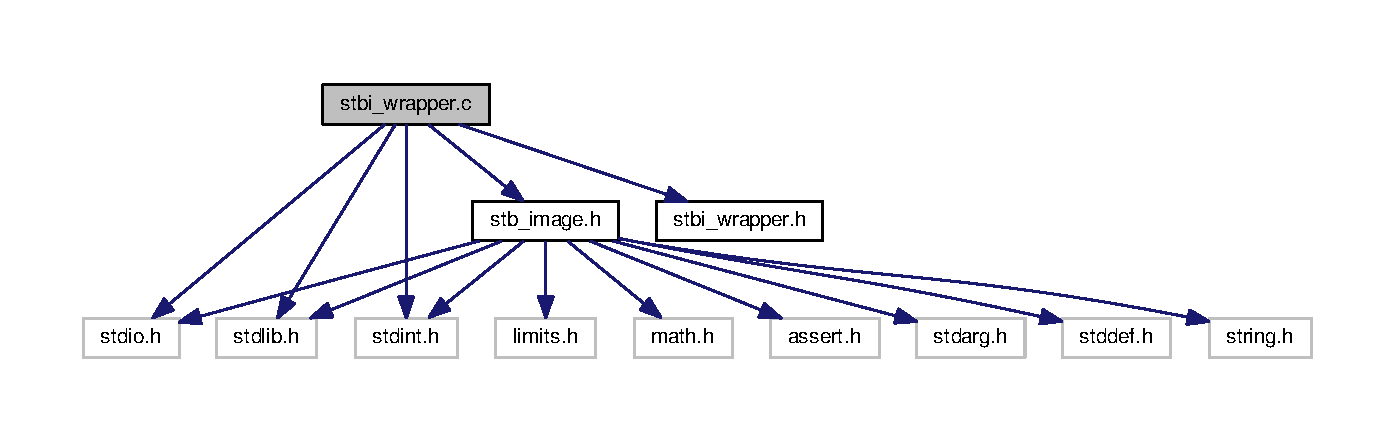
\includegraphics[width=350pt]{stbi__wrapper_8c__incl}
\end{center}
\end{figure}
\subsection*{Macros}
\begin{DoxyCompactItemize}
\item 
\#define \hyperlink{stbi__wrapper_8c_a305f0db3256dd1248d3f17a83f7a6129}{S\+T\+B\+I\+\_\+\+O\+N\+L\+Y\+\_\+\+P\+NG}
\item 
\#define \hyperlink{stbi__wrapper_8c_a18372412ad2fc3ce1e3240b3cf0efe78}{S\+T\+B\+\_\+\+I\+M\+A\+G\+E\+\_\+\+I\+M\+P\+L\+E\+M\+E\+N\+T\+A\+T\+I\+ON}
\end{DoxyCompactItemize}
\subsection*{Functions}
\begin{DoxyCompactItemize}
\item 
unsigned char $\ast$ \hyperlink{stbi__wrapper_8c_a3b92f0f5303b1aa95b7504c27cdf25c9}{stbi\+\_\+png\+\_\+load} (int $\ast$width, int $\ast$height, const char $\ast$image\+\_\+path)
\item 
void \hyperlink{stbi__wrapper_8c_a69419313c4e78cb8556180c6327ffb8c}{stbi\+\_\+free} (unsigned char $\ast$image)
\end{DoxyCompactItemize}


\subsection{Macro Definition Documentation}
\index{stbi\+\_\+wrapper.\+c@{stbi\+\_\+wrapper.\+c}!S\+T\+B\+\_\+\+I\+M\+A\+G\+E\+\_\+\+I\+M\+P\+L\+E\+M\+E\+N\+T\+A\+T\+I\+ON@{S\+T\+B\+\_\+\+I\+M\+A\+G\+E\+\_\+\+I\+M\+P\+L\+E\+M\+E\+N\+T\+A\+T\+I\+ON}}
\index{S\+T\+B\+\_\+\+I\+M\+A\+G\+E\+\_\+\+I\+M\+P\+L\+E\+M\+E\+N\+T\+A\+T\+I\+ON@{S\+T\+B\+\_\+\+I\+M\+A\+G\+E\+\_\+\+I\+M\+P\+L\+E\+M\+E\+N\+T\+A\+T\+I\+ON}!stbi\+\_\+wrapper.\+c@{stbi\+\_\+wrapper.\+c}}
\subsubsection[{\texorpdfstring{S\+T\+B\+\_\+\+I\+M\+A\+G\+E\+\_\+\+I\+M\+P\+L\+E\+M\+E\+N\+T\+A\+T\+I\+ON}{STB_IMAGE_IMPLEMENTATION}}]{\setlength{\rightskip}{0pt plus 5cm}\#define S\+T\+B\+\_\+\+I\+M\+A\+G\+E\+\_\+\+I\+M\+P\+L\+E\+M\+E\+N\+T\+A\+T\+I\+ON}\hypertarget{stbi__wrapper_8c_a18372412ad2fc3ce1e3240b3cf0efe78}{}\label{stbi__wrapper_8c_a18372412ad2fc3ce1e3240b3cf0efe78}
\index{stbi\+\_\+wrapper.\+c@{stbi\+\_\+wrapper.\+c}!S\+T\+B\+I\+\_\+\+O\+N\+L\+Y\+\_\+\+P\+NG@{S\+T\+B\+I\+\_\+\+O\+N\+L\+Y\+\_\+\+P\+NG}}
\index{S\+T\+B\+I\+\_\+\+O\+N\+L\+Y\+\_\+\+P\+NG@{S\+T\+B\+I\+\_\+\+O\+N\+L\+Y\+\_\+\+P\+NG}!stbi\+\_\+wrapper.\+c@{stbi\+\_\+wrapper.\+c}}
\subsubsection[{\texorpdfstring{S\+T\+B\+I\+\_\+\+O\+N\+L\+Y\+\_\+\+P\+NG}{STBI_ONLY_PNG}}]{\setlength{\rightskip}{0pt plus 5cm}\#define S\+T\+B\+I\+\_\+\+O\+N\+L\+Y\+\_\+\+P\+NG}\hypertarget{stbi__wrapper_8c_a305f0db3256dd1248d3f17a83f7a6129}{}\label{stbi__wrapper_8c_a305f0db3256dd1248d3f17a83f7a6129}


\subsection{Function Documentation}
\index{stbi\+\_\+wrapper.\+c@{stbi\+\_\+wrapper.\+c}!stbi\+\_\+free@{stbi\+\_\+free}}
\index{stbi\+\_\+free@{stbi\+\_\+free}!stbi\+\_\+wrapper.\+c@{stbi\+\_\+wrapper.\+c}}
\subsubsection[{\texorpdfstring{stbi\+\_\+free(unsigned char $\ast$image)}{stbi_free(unsigned char *image)}}]{\setlength{\rightskip}{0pt plus 5cm}void stbi\+\_\+free (
\begin{DoxyParamCaption}
\item[{unsigned char $\ast$}]{image}
\end{DoxyParamCaption}
)}\hypertarget{stbi__wrapper_8c_a69419313c4e78cb8556180c6327ffb8c}{}\label{stbi__wrapper_8c_a69419313c4e78cb8556180c6327ffb8c}


Here is the call graph for this function\+:
\nopagebreak
\begin{figure}[H]
\begin{center}
\leavevmode
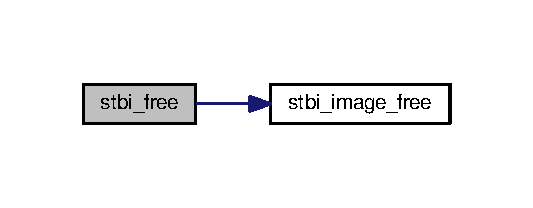
\includegraphics[width=256pt]{stbi__wrapper_8c_a69419313c4e78cb8556180c6327ffb8c_cgraph}
\end{center}
\end{figure}


\index{stbi\+\_\+wrapper.\+c@{stbi\+\_\+wrapper.\+c}!stbi\+\_\+png\+\_\+load@{stbi\+\_\+png\+\_\+load}}
\index{stbi\+\_\+png\+\_\+load@{stbi\+\_\+png\+\_\+load}!stbi\+\_\+wrapper.\+c@{stbi\+\_\+wrapper.\+c}}
\subsubsection[{\texorpdfstring{stbi\+\_\+png\+\_\+load(int $\ast$width, int $\ast$height, const char $\ast$image\+\_\+path)}{stbi_png_load(int *width, int *height, const char *image_path)}}]{\setlength{\rightskip}{0pt plus 5cm}unsigned char$\ast$ stbi\+\_\+png\+\_\+load (
\begin{DoxyParamCaption}
\item[{int $\ast$}]{width, }
\item[{int $\ast$}]{height, }
\item[{const char $\ast$}]{image\+\_\+path}
\end{DoxyParamCaption}
)}\hypertarget{stbi__wrapper_8c_a3b92f0f5303b1aa95b7504c27cdf25c9}{}\label{stbi__wrapper_8c_a3b92f0f5303b1aa95b7504c27cdf25c9}


Here is the call graph for this function\+:
\nopagebreak
\begin{figure}[H]
\begin{center}
\leavevmode
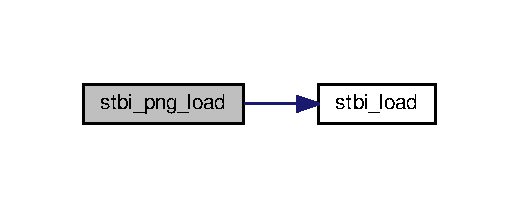
\includegraphics[width=249pt]{stbi__wrapper_8c_a3b92f0f5303b1aa95b7504c27cdf25c9_cgraph}
\end{center}
\end{figure}



\hypertarget{stbi__wrapper_8h}{}\section{stbi\+\_\+wrapper.\+h File Reference}
\label{stbi__wrapper_8h}\index{stbi\+\_\+wrapper.\+h@{stbi\+\_\+wrapper.\+h}}
This graph shows which files directly or indirectly include this file\+:
\nopagebreak
\begin{figure}[H]
\begin{center}
\leavevmode
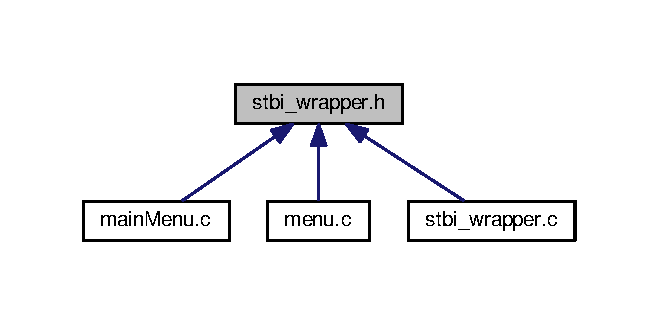
\includegraphics[width=316pt]{stbi__wrapper_8h__dep__incl}
\end{center}
\end{figure}
\subsection*{Functions}
\begin{DoxyCompactItemize}
\item 
unsigned char $\ast$ \hyperlink{stbi__wrapper_8h_a3b92f0f5303b1aa95b7504c27cdf25c9}{stbi\+\_\+png\+\_\+load} (int $\ast$width, int $\ast$height, const char $\ast$image\+\_\+path)
\item 
void \hyperlink{stbi__wrapper_8h_a69419313c4e78cb8556180c6327ffb8c}{stbi\+\_\+free} (unsigned char $\ast$image)
\end{DoxyCompactItemize}


\subsection{Function Documentation}
\index{stbi\+\_\+wrapper.\+h@{stbi\+\_\+wrapper.\+h}!stbi\+\_\+free@{stbi\+\_\+free}}
\index{stbi\+\_\+free@{stbi\+\_\+free}!stbi\+\_\+wrapper.\+h@{stbi\+\_\+wrapper.\+h}}
\subsubsection[{\texorpdfstring{stbi\+\_\+free(unsigned char $\ast$image)}{stbi_free(unsigned char *image)}}]{\setlength{\rightskip}{0pt plus 5cm}void stbi\+\_\+free (
\begin{DoxyParamCaption}
\item[{unsigned char $\ast$}]{image}
\end{DoxyParamCaption}
)}\hypertarget{stbi__wrapper_8h_a69419313c4e78cb8556180c6327ffb8c}{}\label{stbi__wrapper_8h_a69419313c4e78cb8556180c6327ffb8c}


Here is the call graph for this function\+:
\nopagebreak
\begin{figure}[H]
\begin{center}
\leavevmode
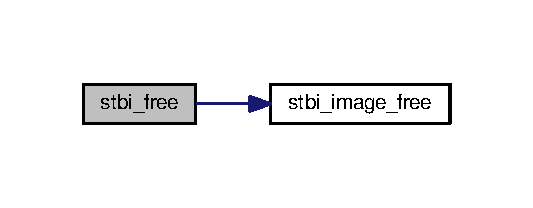
\includegraphics[width=256pt]{stbi__wrapper_8h_a69419313c4e78cb8556180c6327ffb8c_cgraph}
\end{center}
\end{figure}


\index{stbi\+\_\+wrapper.\+h@{stbi\+\_\+wrapper.\+h}!stbi\+\_\+png\+\_\+load@{stbi\+\_\+png\+\_\+load}}
\index{stbi\+\_\+png\+\_\+load@{stbi\+\_\+png\+\_\+load}!stbi\+\_\+wrapper.\+h@{stbi\+\_\+wrapper.\+h}}
\subsubsection[{\texorpdfstring{stbi\+\_\+png\+\_\+load(int $\ast$width, int $\ast$height, const char $\ast$image\+\_\+path)}{stbi_png_load(int *width, int *height, const char *image_path)}}]{\setlength{\rightskip}{0pt plus 5cm}unsigned char$\ast$ stbi\+\_\+png\+\_\+load (
\begin{DoxyParamCaption}
\item[{int $\ast$}]{width, }
\item[{int $\ast$}]{height, }
\item[{const char $\ast$}]{image\+\_\+path}
\end{DoxyParamCaption}
)}\hypertarget{stbi__wrapper_8h_a3b92f0f5303b1aa95b7504c27cdf25c9}{}\label{stbi__wrapper_8h_a3b92f0f5303b1aa95b7504c27cdf25c9}


Here is the call graph for this function\+:
\nopagebreak
\begin{figure}[H]
\begin{center}
\leavevmode
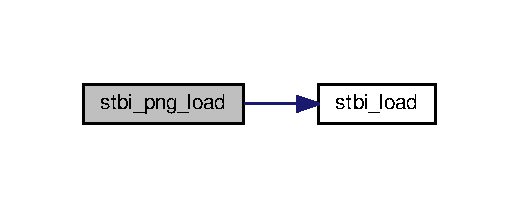
\includegraphics[width=249pt]{stbi__wrapper_8h_a3b92f0f5303b1aa95b7504c27cdf25c9_cgraph}
\end{center}
\end{figure}



\hypertarget{timer_8c}{}\section{timer.\+c File Reference}
\label{timer_8c}\index{timer.\+c@{timer.\+c}}
{\ttfamily \#include $<$minix/syslib.\+h$>$}\\*
{\ttfamily \#include $<$minix/drivers.\+h$>$}\\*
{\ttfamily \#include $<$minix/driver.\+h$>$}\\*
{\ttfamily \#include $<$minix/com.\+h$>$}\\*
{\ttfamily \#include \char`\"{}i8254.\+h\char`\"{}}\\*
{\ttfamily \#include \char`\"{}timer.\+h\char`\"{}}\\*
Include dependency graph for timer.\+c\+:
\nopagebreak
\begin{figure}[H]
\begin{center}
\leavevmode
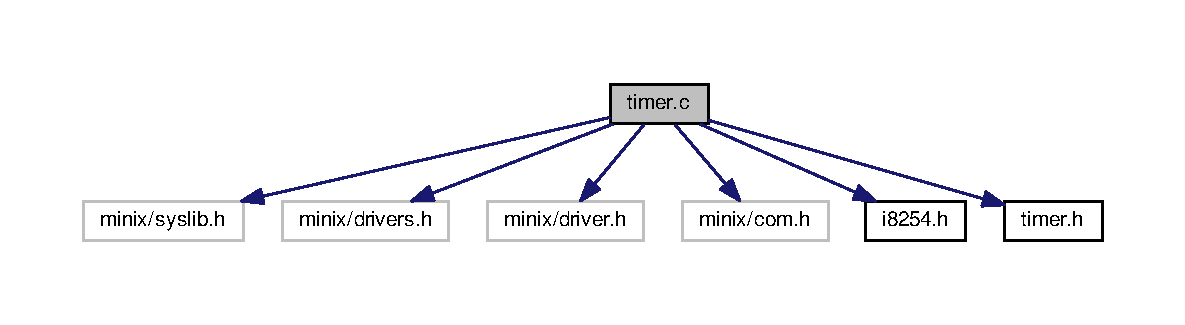
\includegraphics[width=350pt]{timer_8c__incl}
\end{center}
\end{figure}
\subsection*{Functions}
\begin{DoxyCompactItemize}
\item 
int \hyperlink{group__timer_ga4c5d9f47323eda494cfd826f6d62eec9}{timer\+\_\+subscribe\+\_\+int} (void)
\begin{DoxyCompactList}\small\item\em Subscribes and enables Timer 0 interrupts. \end{DoxyCompactList}\item 
int \hyperlink{group__timer_gab9eea51549744bca5c5c923b388bb4ee}{timer\+\_\+unsubscribe\+\_\+int} ()
\begin{DoxyCompactList}\small\item\em Unsubscribes Timer 0 interrupts. \end{DoxyCompactList}\item 
void \hyperlink{group__timer_ga10fc9c867b15c7da6649311c9987cd17}{timer\+\_\+int\+\_\+handler} ()
\begin{DoxyCompactList}\small\item\em Timer 0 interrupt handler. \end{DoxyCompactList}\end{DoxyCompactItemize}
\subsection*{Variables}
\begin{DoxyCompactItemize}
\item 
static int \hyperlink{timer_8c_a1006f2cc60be47c618c0a058896ce1e6}{hook\+ID} = 0
\item 
int \hyperlink{group__timer_ga617a47c70795bcff659815ad0efd2266}{counter} = 0
\end{DoxyCompactItemize}


\subsection{Variable Documentation}
\index{timer.\+c@{timer.\+c}!hook\+ID@{hook\+ID}}
\index{hook\+ID@{hook\+ID}!timer.\+c@{timer.\+c}}
\subsubsection[{\texorpdfstring{hook\+ID}{hookID}}]{\setlength{\rightskip}{0pt plus 5cm}int hook\+ID = 0\hspace{0.3cm}{\ttfamily [static]}}\hypertarget{timer_8c_a1006f2cc60be47c618c0a058896ce1e6}{}\label{timer_8c_a1006f2cc60be47c618c0a058896ce1e6}

\hypertarget{timer_8h}{}\section{timer.\+h File Reference}
\label{timer_8h}\index{timer.\+h@{timer.\+h}}
This graph shows which files directly or indirectly include this file\+:
\nopagebreak
\begin{figure}[H]
\begin{center}
\leavevmode
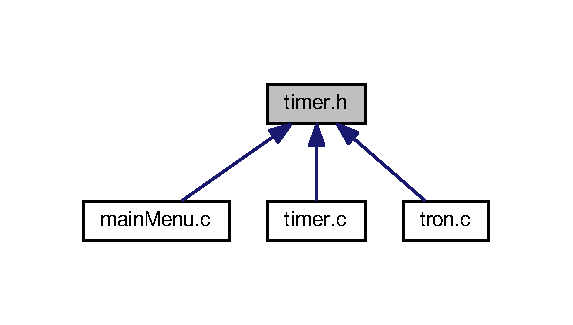
\includegraphics[width=275pt]{timer_8h__dep__incl}
\end{center}
\end{figure}
\subsection*{Functions}
\begin{DoxyCompactItemize}
\item 
int \hyperlink{group__timer_ga4c5d9f47323eda494cfd826f6d62eec9}{timer\+\_\+subscribe\+\_\+int} (void)
\begin{DoxyCompactList}\small\item\em Subscribes and enables Timer 0 interrupts. \end{DoxyCompactList}\item 
int \hyperlink{group__timer_gab9eea51549744bca5c5c923b388bb4ee}{timer\+\_\+unsubscribe\+\_\+int} ()
\begin{DoxyCompactList}\small\item\em Unsubscribes Timer 0 interrupts. \end{DoxyCompactList}\item 
void \hyperlink{group__timer_ga10fc9c867b15c7da6649311c9987cd17}{timer\+\_\+int\+\_\+handler} ()
\begin{DoxyCompactList}\small\item\em Timer 0 interrupt handler. \end{DoxyCompactList}\end{DoxyCompactItemize}
\subsection*{Variables}
\begin{DoxyCompactItemize}
\item 
int \hyperlink{group__timer_ga617a47c70795bcff659815ad0efd2266}{counter}
\end{DoxyCompactItemize}

\hypertarget{tron_8c}{}\section{tron.\+c File Reference}
\label{tron_8c}\index{tron.\+c@{tron.\+c}}
{\ttfamily \#include $<$minix/drivers.\+h$>$}\\*
{\ttfamily \#include $<$minix/syslib.\+h$>$}\\*
{\ttfamily \#include $<$minix/driver.\+h$>$}\\*
{\ttfamily \#include $<$minix/com.\+h$>$}\\*
{\ttfamily \#include $<$minix/sysutil.\+h$>$}\\*
{\ttfamily \#include $<$limits.\+h$>$}\\*
{\ttfamily \#include $<$string.\+h$>$}\\*
{\ttfamily \#include $<$errno.\+h$>$}\\*
{\ttfamily \#include $<$stdio.\+h$>$}\\*
{\ttfamily \#include $<$math.\+h$>$}\\*
{\ttfamily \#include \char`\"{}video\+\_\+gr.\+h\char`\"{}}\\*
{\ttfamily \#include \char`\"{}keyboard.\+h\char`\"{}}\\*
{\ttfamily \#include \char`\"{}mouse.\+h\char`\"{}}\\*
{\ttfamily \#include \char`\"{}i8042.\+h\char`\"{}}\\*
{\ttfamily \#include \char`\"{}timer.\+h\char`\"{}}\\*
{\ttfamily \#include \char`\"{}i8254.\+h\char`\"{}}\\*
{\ttfamily \#include \char`\"{}bike.\+h\char`\"{}}\\*
Include dependency graph for tron.\+c\+:
\nopagebreak
\begin{figure}[H]
\begin{center}
\leavevmode
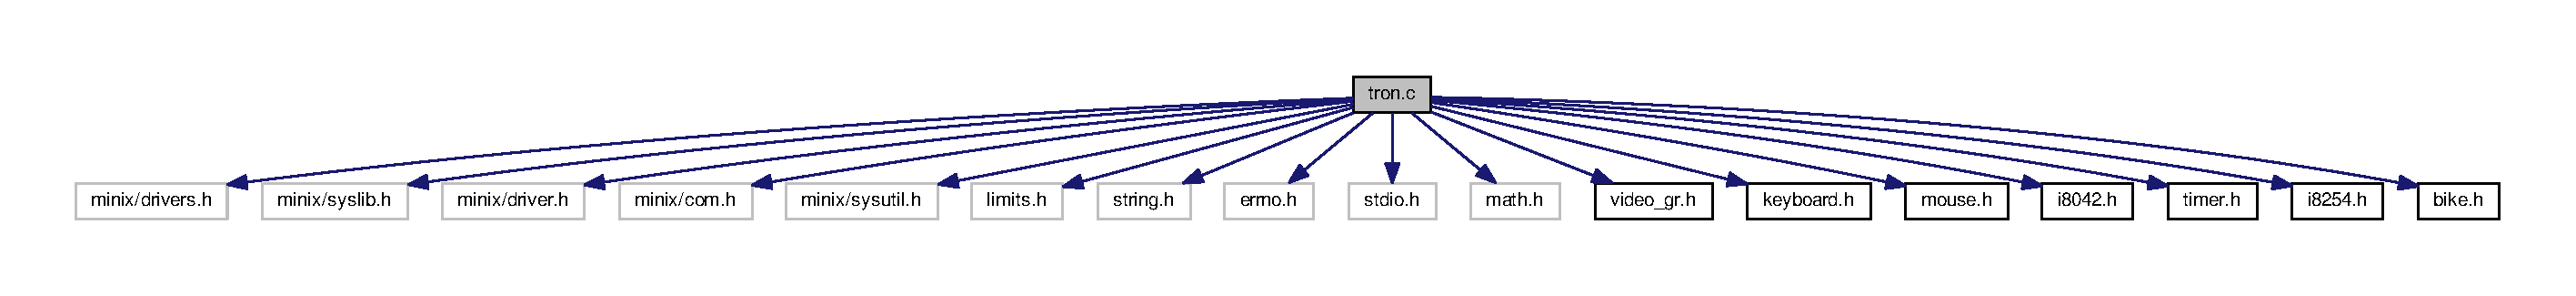
\includegraphics[width=350pt]{tron_8c__incl}
\end{center}
\end{figure}
\subsection*{Functions}
\begin{DoxyCompactItemize}
\item 
int \hyperlink{tron_8c_a03e7dcdcb72c488e797b70a6e205ffc4}{check\+Screen\+Border} (\hyperlink{structBike}{Bike} bike)
\item 
int \hyperlink{tron_8c_ae84c69a9097130cb9f97b2846961aab2}{check\+Colision} (\hyperlink{structBike}{Bike} bike)
\item 
int \hyperlink{tron_8c_aee51a9a5905e3abd702655d499cc900a}{play\+Tron} ()
\end{DoxyCompactItemize}
\subsection*{Variables}
\begin{DoxyCompactItemize}
\item 
int \hyperlink{tron_8c_ac3897a350075920efc6bab8d04cc1215}{winner}
\end{DoxyCompactItemize}


\subsection{Function Documentation}
\index{tron.\+c@{tron.\+c}!check\+Colision@{check\+Colision}}
\index{check\+Colision@{check\+Colision}!tron.\+c@{tron.\+c}}
\subsubsection[{\texorpdfstring{check\+Colision(\+Bike bike)}{checkColision(Bike bike)}}]{\setlength{\rightskip}{0pt plus 5cm}int check\+Colision (
\begin{DoxyParamCaption}
\item[{{\bf Bike}}]{bike}
\end{DoxyParamCaption}
)}\hypertarget{tron_8c_ae84c69a9097130cb9f97b2846961aab2}{}\label{tron_8c_ae84c69a9097130cb9f97b2846961aab2}


Here is the call graph for this function\+:
\nopagebreak
\begin{figure}[H]
\begin{center}
\leavevmode
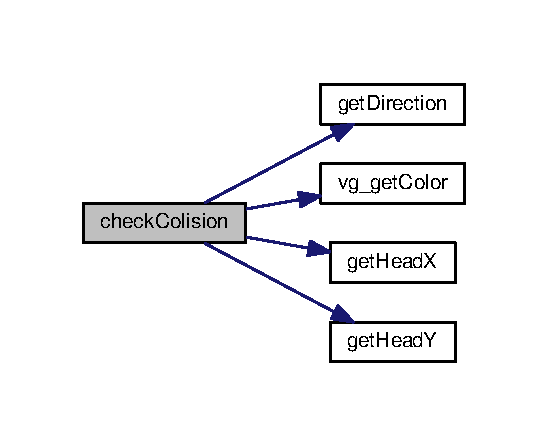
\includegraphics[width=263pt]{tron_8c_ae84c69a9097130cb9f97b2846961aab2_cgraph}
\end{center}
\end{figure}


\index{tron.\+c@{tron.\+c}!check\+Screen\+Border@{check\+Screen\+Border}}
\index{check\+Screen\+Border@{check\+Screen\+Border}!tron.\+c@{tron.\+c}}
\subsubsection[{\texorpdfstring{check\+Screen\+Border(\+Bike bike)}{checkScreenBorder(Bike bike)}}]{\setlength{\rightskip}{0pt plus 5cm}int check\+Screen\+Border (
\begin{DoxyParamCaption}
\item[{{\bf Bike}}]{bike}
\end{DoxyParamCaption}
)}\hypertarget{tron_8c_a03e7dcdcb72c488e797b70a6e205ffc4}{}\label{tron_8c_a03e7dcdcb72c488e797b70a6e205ffc4}


Here is the call graph for this function\+:
\nopagebreak
\begin{figure}[H]
\begin{center}
\leavevmode
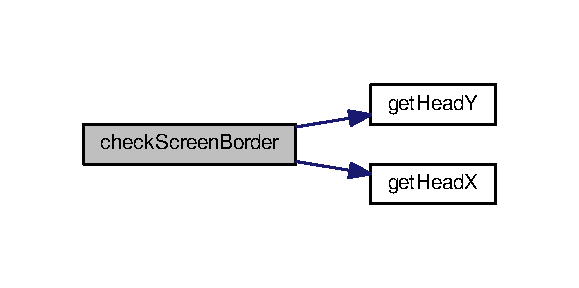
\includegraphics[width=278pt]{tron_8c_a03e7dcdcb72c488e797b70a6e205ffc4_cgraph}
\end{center}
\end{figure}


\index{tron.\+c@{tron.\+c}!play\+Tron@{play\+Tron}}
\index{play\+Tron@{play\+Tron}!tron.\+c@{tron.\+c}}
\subsubsection[{\texorpdfstring{play\+Tron()}{playTron()}}]{\setlength{\rightskip}{0pt plus 5cm}int play\+Tron (
\begin{DoxyParamCaption}
{}
\end{DoxyParamCaption}
)}\hypertarget{tron_8c_aee51a9a5905e3abd702655d499cc900a}{}\label{tron_8c_aee51a9a5905e3abd702655d499cc900a}


Here is the call graph for this function\+:
\nopagebreak
\begin{figure}[H]
\begin{center}
\leavevmode
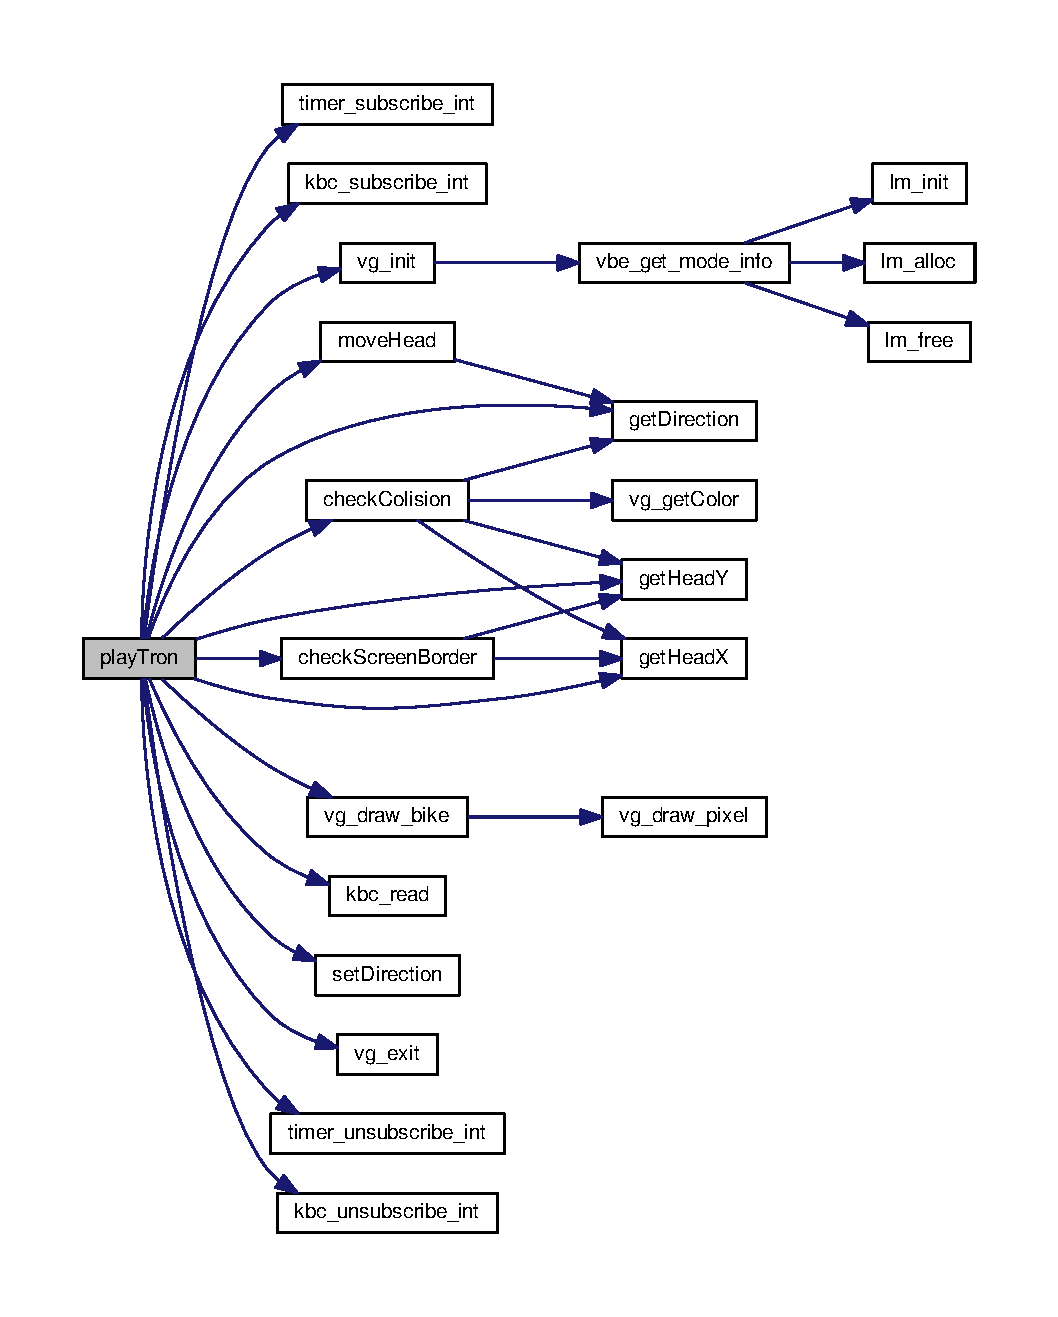
\includegraphics[width=350pt]{tron_8c_aee51a9a5905e3abd702655d499cc900a_cgraph}
\end{center}
\end{figure}




\subsection{Variable Documentation}
\index{tron.\+c@{tron.\+c}!winner@{winner}}
\index{winner@{winner}!tron.\+c@{tron.\+c}}
\subsubsection[{\texorpdfstring{winner}{winner}}]{\setlength{\rightskip}{0pt plus 5cm}int winner}\hypertarget{tron_8c_ac3897a350075920efc6bab8d04cc1215}{}\label{tron_8c_ac3897a350075920efc6bab8d04cc1215}

\hypertarget{tron_8h}{}\section{tron.\+h File Reference}
\label{tron_8h}\index{tron.\+h@{tron.\+h}}
{\ttfamily \#include \char`\"{}bike.\+h\char`\"{}}\\*
Include dependency graph for tron.\+h\+:
\nopagebreak
\begin{figure}[H]
\begin{center}
\leavevmode
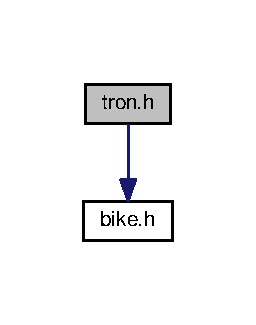
\includegraphics[width=123pt]{tron_8h__incl}
\end{center}
\end{figure}
This graph shows which files directly or indirectly include this file\+:
\nopagebreak
\begin{figure}[H]
\begin{center}
\leavevmode
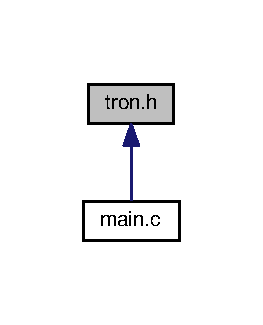
\includegraphics[width=126pt]{tron_8h__dep__incl}
\end{center}
\end{figure}
\subsection*{Functions}
\begin{DoxyCompactItemize}
\item 
int \hyperlink{tron_8h_a03e7dcdcb72c488e797b70a6e205ffc4}{check\+Screen\+Border} (\hyperlink{structBike}{Bike} bike)
\item 
int \hyperlink{tron_8h_ae84c69a9097130cb9f97b2846961aab2}{check\+Colision} (\hyperlink{structBike}{Bike} bike)
\item 
int \hyperlink{tron_8h_aee51a9a5905e3abd702655d499cc900a}{play\+Tron} ()
\end{DoxyCompactItemize}


\subsection{Function Documentation}
\index{tron.\+h@{tron.\+h}!check\+Colision@{check\+Colision}}
\index{check\+Colision@{check\+Colision}!tron.\+h@{tron.\+h}}
\subsubsection[{\texorpdfstring{check\+Colision(\+Bike bike)}{checkColision(Bike bike)}}]{\setlength{\rightskip}{0pt plus 5cm}int check\+Colision (
\begin{DoxyParamCaption}
\item[{{\bf Bike}}]{bike}
\end{DoxyParamCaption}
)}\hypertarget{tron_8h_ae84c69a9097130cb9f97b2846961aab2}{}\label{tron_8h_ae84c69a9097130cb9f97b2846961aab2}


Here is the call graph for this function\+:
\nopagebreak
\begin{figure}[H]
\begin{center}
\leavevmode
\includegraphics[width=263pt]{tron_8h_ae84c69a9097130cb9f97b2846961aab2_cgraph}
\end{center}
\end{figure}


\index{tron.\+h@{tron.\+h}!check\+Screen\+Border@{check\+Screen\+Border}}
\index{check\+Screen\+Border@{check\+Screen\+Border}!tron.\+h@{tron.\+h}}
\subsubsection[{\texorpdfstring{check\+Screen\+Border(\+Bike bike)}{checkScreenBorder(Bike bike)}}]{\setlength{\rightskip}{0pt plus 5cm}int check\+Screen\+Border (
\begin{DoxyParamCaption}
\item[{{\bf Bike}}]{bike}
\end{DoxyParamCaption}
)}\hypertarget{tron_8h_a03e7dcdcb72c488e797b70a6e205ffc4}{}\label{tron_8h_a03e7dcdcb72c488e797b70a6e205ffc4}


Here is the call graph for this function\+:
\nopagebreak
\begin{figure}[H]
\begin{center}
\leavevmode
\includegraphics[width=278pt]{tron_8h_a03e7dcdcb72c488e797b70a6e205ffc4_cgraph}
\end{center}
\end{figure}


\index{tron.\+h@{tron.\+h}!play\+Tron@{play\+Tron}}
\index{play\+Tron@{play\+Tron}!tron.\+h@{tron.\+h}}
\subsubsection[{\texorpdfstring{play\+Tron()}{playTron()}}]{\setlength{\rightskip}{0pt plus 5cm}int play\+Tron (
\begin{DoxyParamCaption}
{}
\end{DoxyParamCaption}
)}\hypertarget{tron_8h_aee51a9a5905e3abd702655d499cc900a}{}\label{tron_8h_aee51a9a5905e3abd702655d499cc900a}


Here is the call graph for this function\+:
\nopagebreak
\begin{figure}[H]
\begin{center}
\leavevmode
\includegraphics[width=350pt]{tron_8h_aee51a9a5905e3abd702655d499cc900a_cgraph}
\end{center}
\end{figure}



\hypertarget{vbe_8c}{}\section{vbe.\+c File Reference}
\label{vbe_8c}\index{vbe.\+c@{vbe.\+c}}
{\ttfamily \#include $<$minix/syslib.\+h$>$}\\*
{\ttfamily \#include $<$minix/drivers.\+h$>$}\\*
{\ttfamily \#include $<$machine/int86.\+h$>$}\\*
{\ttfamily \#include \char`\"{}vbe.\+h\char`\"{}}\\*
{\ttfamily \#include \char`\"{}lmlib.\+h\char`\"{}}\\*
{\ttfamily \#include \char`\"{}video.\+h\char`\"{}}\\*
Include dependency graph for vbe.\+c\+:
\nopagebreak
\begin{figure}[H]
\begin{center}
\leavevmode
\includegraphics[width=350pt]{vbe_8c__incl}
\end{center}
\end{figure}
\subsection*{Macros}
\begin{DoxyCompactItemize}
\item 
\#define \hyperlink{vbe_8c_a0007120a310d0ec70307f51f43eb81a3}{L\+I\+N\+E\+A\+R\+\_\+\+M\+O\+D\+E\+L\+\_\+\+B\+IT}~14
\item 
\#define \hyperlink{vbe_8c_a68b87c2339cb305d66b69b5551b96c73}{P\+B2\+B\+A\+SE}(x)~(((x) $>$$>$ 4) \& 0x0\+F000)
\item 
\#define \hyperlink{vbe_8c_a70c65ed4c6d71865daa96d31befb33fd}{P\+B2\+O\+FF}(x)~((x) \& 0x0\+F\+F\+F\+F)
\end{DoxyCompactItemize}
\subsection*{Functions}
\begin{DoxyCompactItemize}
\item 
int \hyperlink{group__vbe_ga4ef3234e41f2050bc094a22049b69e45}{vbe\+\_\+get\+\_\+mode\+\_\+info} (unsigned short mode, vbe\+\_\+mode\+\_\+info\+\_\+t $\ast$vmi\+\_\+p)
\begin{DoxyCompactList}\small\item\em Returns information on the input V\+BE mode, including screen dimensions, color depth and V\+R\+AM physical address. \end{DoxyCompactList}\end{DoxyCompactItemize}


\subsection{Macro Definition Documentation}
\index{vbe.\+c@{vbe.\+c}!L\+I\+N\+E\+A\+R\+\_\+\+M\+O\+D\+E\+L\+\_\+\+B\+IT@{L\+I\+N\+E\+A\+R\+\_\+\+M\+O\+D\+E\+L\+\_\+\+B\+IT}}
\index{L\+I\+N\+E\+A\+R\+\_\+\+M\+O\+D\+E\+L\+\_\+\+B\+IT@{L\+I\+N\+E\+A\+R\+\_\+\+M\+O\+D\+E\+L\+\_\+\+B\+IT}!vbe.\+c@{vbe.\+c}}
\subsubsection[{\texorpdfstring{L\+I\+N\+E\+A\+R\+\_\+\+M\+O\+D\+E\+L\+\_\+\+B\+IT}{LINEAR_MODEL_BIT}}]{\setlength{\rightskip}{0pt plus 5cm}\#define L\+I\+N\+E\+A\+R\+\_\+\+M\+O\+D\+E\+L\+\_\+\+B\+IT~14}\hypertarget{vbe_8c_a0007120a310d0ec70307f51f43eb81a3}{}\label{vbe_8c_a0007120a310d0ec70307f51f43eb81a3}
\index{vbe.\+c@{vbe.\+c}!P\+B2\+B\+A\+SE@{P\+B2\+B\+A\+SE}}
\index{P\+B2\+B\+A\+SE@{P\+B2\+B\+A\+SE}!vbe.\+c@{vbe.\+c}}
\subsubsection[{\texorpdfstring{P\+B2\+B\+A\+SE}{PB2BASE}}]{\setlength{\rightskip}{0pt plus 5cm}\#define P\+B2\+B\+A\+SE(
\begin{DoxyParamCaption}
\item[{}]{x}
\end{DoxyParamCaption}
)~(((x) $>$$>$ 4) \& 0x0\+F000)}\hypertarget{vbe_8c_a68b87c2339cb305d66b69b5551b96c73}{}\label{vbe_8c_a68b87c2339cb305d66b69b5551b96c73}
\index{vbe.\+c@{vbe.\+c}!P\+B2\+O\+FF@{P\+B2\+O\+FF}}
\index{P\+B2\+O\+FF@{P\+B2\+O\+FF}!vbe.\+c@{vbe.\+c}}
\subsubsection[{\texorpdfstring{P\+B2\+O\+FF}{PB2OFF}}]{\setlength{\rightskip}{0pt plus 5cm}\#define P\+B2\+O\+FF(
\begin{DoxyParamCaption}
\item[{}]{x}
\end{DoxyParamCaption}
)~((x) \& 0x0\+F\+F\+F\+F)}\hypertarget{vbe_8c_a70c65ed4c6d71865daa96d31befb33fd}{}\label{vbe_8c_a70c65ed4c6d71865daa96d31befb33fd}

\hypertarget{vbe_8h}{}\section{vbe.\+h File Reference}
\label{vbe_8h}\index{vbe.\+h@{vbe.\+h}}
{\ttfamily \#include $<$stdint.\+h$>$}\\*
{\ttfamily \#include \char`\"{}lmlib.\+h\char`\"{}}\\*
Include dependency graph for vbe.\+h\+:
\nopagebreak
\begin{figure}[H]
\begin{center}
\leavevmode
\includegraphics[width=192pt]{vbe_8h__incl}
\end{center}
\end{figure}
This graph shows which files directly or indirectly include this file\+:
\nopagebreak
\begin{figure}[H]
\begin{center}
\leavevmode
\includegraphics[width=202pt]{vbe_8h__dep__incl}
\end{center}
\end{figure}
\subsection*{Classes}
\begin{DoxyCompactItemize}
\item 
struct \hyperlink{struct____attribute____}{\+\_\+\+\_\+attribute\+\_\+\+\_\+}
\end{DoxyCompactItemize}
\subsection*{Functions}
\begin{DoxyCompactItemize}
\item 
int \hyperlink{group__vbe_ga4ef3234e41f2050bc094a22049b69e45}{vbe\+\_\+get\+\_\+mode\+\_\+info} (unsigned short mode, vbe\+\_\+mode\+\_\+info\+\_\+t $\ast$vmi\+\_\+p)
\begin{DoxyCompactList}\small\item\em Returns information on the input V\+BE mode, including screen dimensions, color depth and V\+R\+AM physical address. \end{DoxyCompactList}\end{DoxyCompactItemize}

\hypertarget{video_8h}{}\section{video.\+h File Reference}
\label{video_8h}\index{video.\+h@{video.\+h}}
This graph shows which files directly or indirectly include this file\+:
\nopagebreak
\begin{figure}[H]
\begin{center}
\leavevmode
\includegraphics[width=202pt]{video_8h__dep__incl}
\end{center}
\end{figure}
\subsection*{Macros}
\begin{DoxyCompactItemize}
\item 
\#define \hyperlink{video_8h_a3a8ea58898cb58fc96013383d39f482c}{B\+IT}(n)~(0x01$<$$<$(n))
\item 
\#define \hyperlink{video_8h_a68b87c2339cb305d66b69b5551b96c73}{P\+B2\+B\+A\+SE}(x)~(((x) $>$$>$ 4) \& 0x0\+F000)
\item 
\#define \hyperlink{video_8h_a70c65ed4c6d71865daa96d31befb33fd}{P\+B2\+O\+FF}(x)~((x) \& 0x0\+F\+F\+F\+F)
\item 
\#define \hyperlink{video_8h_a45ba202b05caf39795aeca91b0ae547e}{T\+I\+M\+E\+O\+UT}~3
\item 
\#define \hyperlink{video_8h_aa8cecfc5c5c054d2875c03e77b7be15d}{T\+R\+UE}~0x01
\item 
\#define \hyperlink{video_8h_aa93f0eb578d23995850d61f7d61c55c1}{F\+A\+L\+SE}~0x00
\item 
\#define \hyperlink{video_8h_ac854e8352d97c69bdfe247573593ba3b}{V\+R\+A\+M\+\_\+\+P\+H\+Y\+S\+\_\+\+A\+D\+DR}~0x\+E0000000
\item 
\#define \hyperlink{video_8h_a0b5a72e5bc312b2cfa60c5b37c29752b}{V\+R\+A\+M\+\_\+\+P\+H\+Y\+S\+\_\+\+A\+D\+D\+R\+\_\+T}~0x\+D\+C000000
\item 
\#define \hyperlink{video_8h_abf6f66114c31b8f87c80534ca695a00b}{H\+\_\+\+R\+ES}~1024
\item 
\#define \hyperlink{video_8h_aac2466862bcfc18231c38fe1eacc22e3}{V\+\_\+\+R\+ES}~768
\item 
\#define \hyperlink{video_8h_a35faf89171af20cd21088c37d62bb7ee}{B\+I\+T\+S\+\_\+\+P\+E\+R\+\_\+\+P\+I\+X\+EL}~8
\item 
\#define \hyperlink{video_8h_ab3ae6cab04af0d37663adf157287f987}{V\+B\+E\+\_\+\+C\+O\+N\+T\+R\+O\+L\+L\+E\+R\+\_\+\+I\+N\+FO}~0x4\+F00
\item 
\#define \hyperlink{video_8h_a2ecbf8f92f9322fedec91461747c4843}{V\+B\+E\+\_\+\+M\+O\+D\+E\+\_\+\+I\+N\+FO}~0x4\+F01
\item 
\#define \hyperlink{video_8h_ab32156e1d72cb92b120bb16883c87eea}{S\+E\+T\+\_\+\+V\+B\+E\+\_\+\+M\+O\+DE}~0x4\+F02
\item 
\#define \hyperlink{video_8h_ac28d52edfa71400c06a4ed014eed978d}{B\+I\+O\+S\+\_\+\+V\+I\+D\+EO}~0x10
\item 
\#define \hyperlink{video_8h_adfa40b6e434f64781fe04f9c2ab95f82}{L\+I\+N\+E\+A\+R\+\_\+\+F\+R\+A\+ME}~\hyperlink{video_8h_a3a8ea58898cb58fc96013383d39f482c}{B\+IT}(14)
\item 
\#define \hyperlink{video_8h_a8171ae48500ff706b097a9eb0ab1885d}{M\+O\+D\+E105H}~0x105
\item 
\#define \hyperlink{video_8h_a442adec72b1e1c00e0571f3712dddb0a}{M\+O\+D\+E\+\_\+\+I\+N\+F\+O\+\_\+\+S\+I\+ZE}~256
\item 
\#define \hyperlink{video_8h_a45404c3c762f1e48cf9294137747f1cd}{M\+A\+X\+R\+ES}~1600
\item 
\#define \hyperlink{video_8h_ab26bec893d32a663260966bcb46ed2d0}{M\+A\+X\+R\+E\+S\+\_\+105}~1024
\item 
\#define \hyperlink{video_8h_ac60f8ab11a88ffb1903ac7bb20815b31}{F\+S\+U\+P\+P\+O\+R\+T\+ED}~0x4F
\item 
\#define \hyperlink{video_8h_a072379dfe70dc9cb27062473fe66d1ab}{F\+C\+A\+L\+L\+\_\+\+S\+U\+C\+C\+E\+SS}~0x00
\item 
\#define \hyperlink{video_8h_a43a1eccce2e73811114963475b4db4dd}{F\+C\+A\+L\+L\+\_\+\+F\+A\+IL}~0x01
\item 
\#define \hyperlink{video_8h_a380b9fe21073ebf61328d51cc5b742a6}{F\+H\+A\+R\+D\+W\+A\+RE}~0x02
\item 
\#define \hyperlink{video_8h_a42b2a3ddf65405ccb753984d561566bd}{F\+I\+N\+V\+A\+L\+ID}~0x03
\item 
\#define \hyperlink{video_8h_a2abff7b8f61bfdee3c2fe5cc0da9b713}{V\+I\+D\+E\+O\+M\+O\+D\+E\+P\+TR}~0x00
\item 
\#define \hyperlink{video_8h_acb7036a0f47360d42ee2b9ade3e15131}{V\+B\+E\+\_\+\+R\+E\+S\+E\+R\+V\+ED}~0x01
\item 
\#define \hyperlink{video_8h_a2688910de2afe3a3833d48630252ca00}{B\+O\+T\+H\+\_\+\+M\+O\+D\+ES}~0x02
\item 
\#define \hyperlink{video_8h_ae452d1931f9b23fb1a9750b64afc0f2b}{L\+I\+N\+E\+\_\+\+B\+R\+E\+AK}~12
\item 
\#define \hyperlink{video_8h_a40269eccee35199ba216678b8891ca5a}{R\+E\+S\+E\+R\+V\+E\+D\+\_\+\+S\+I\+ZE}~222
\item 
\#define \hyperlink{video_8h_a7b3b25cba33b07c303f3060fe41887f6}{B\+L\+A\+CK}~0x00
\item 
\#define \hyperlink{video_8h_a87b537f5fa5c109d3c05c13d6b18f382}{W\+H\+I\+TE}~0x3F
\item 
\#define \hyperlink{video_8h_ade7320bfb062b4cbf73aa734f7f28125}{M\+A\+X256}~0x\+FF
\end{DoxyCompactItemize}


\subsection{Macro Definition Documentation}
\index{video.\+h@{video.\+h}!B\+I\+O\+S\+\_\+\+V\+I\+D\+EO@{B\+I\+O\+S\+\_\+\+V\+I\+D\+EO}}
\index{B\+I\+O\+S\+\_\+\+V\+I\+D\+EO@{B\+I\+O\+S\+\_\+\+V\+I\+D\+EO}!video.\+h@{video.\+h}}
\subsubsection[{\texorpdfstring{B\+I\+O\+S\+\_\+\+V\+I\+D\+EO}{BIOS_VIDEO}}]{\setlength{\rightskip}{0pt plus 5cm}\#define B\+I\+O\+S\+\_\+\+V\+I\+D\+EO~0x10}\hypertarget{video_8h_ac28d52edfa71400c06a4ed014eed978d}{}\label{video_8h_ac28d52edfa71400c06a4ed014eed978d}
\index{video.\+h@{video.\+h}!B\+IT@{B\+IT}}
\index{B\+IT@{B\+IT}!video.\+h@{video.\+h}}
\subsubsection[{\texorpdfstring{B\+IT}{BIT}}]{\setlength{\rightskip}{0pt plus 5cm}\#define B\+IT(
\begin{DoxyParamCaption}
\item[{}]{n}
\end{DoxyParamCaption}
)~(0x01$<$$<$(n))}\hypertarget{video_8h_a3a8ea58898cb58fc96013383d39f482c}{}\label{video_8h_a3a8ea58898cb58fc96013383d39f482c}
\index{video.\+h@{video.\+h}!B\+I\+T\+S\+\_\+\+P\+E\+R\+\_\+\+P\+I\+X\+EL@{B\+I\+T\+S\+\_\+\+P\+E\+R\+\_\+\+P\+I\+X\+EL}}
\index{B\+I\+T\+S\+\_\+\+P\+E\+R\+\_\+\+P\+I\+X\+EL@{B\+I\+T\+S\+\_\+\+P\+E\+R\+\_\+\+P\+I\+X\+EL}!video.\+h@{video.\+h}}
\subsubsection[{\texorpdfstring{B\+I\+T\+S\+\_\+\+P\+E\+R\+\_\+\+P\+I\+X\+EL}{BITS_PER_PIXEL}}]{\setlength{\rightskip}{0pt plus 5cm}\#define B\+I\+T\+S\+\_\+\+P\+E\+R\+\_\+\+P\+I\+X\+EL~8}\hypertarget{video_8h_a35faf89171af20cd21088c37d62bb7ee}{}\label{video_8h_a35faf89171af20cd21088c37d62bb7ee}
\index{video.\+h@{video.\+h}!B\+L\+A\+CK@{B\+L\+A\+CK}}
\index{B\+L\+A\+CK@{B\+L\+A\+CK}!video.\+h@{video.\+h}}
\subsubsection[{\texorpdfstring{B\+L\+A\+CK}{BLACK}}]{\setlength{\rightskip}{0pt plus 5cm}\#define B\+L\+A\+CK~0x00}\hypertarget{video_8h_a7b3b25cba33b07c303f3060fe41887f6}{}\label{video_8h_a7b3b25cba33b07c303f3060fe41887f6}
\index{video.\+h@{video.\+h}!B\+O\+T\+H\+\_\+\+M\+O\+D\+ES@{B\+O\+T\+H\+\_\+\+M\+O\+D\+ES}}
\index{B\+O\+T\+H\+\_\+\+M\+O\+D\+ES@{B\+O\+T\+H\+\_\+\+M\+O\+D\+ES}!video.\+h@{video.\+h}}
\subsubsection[{\texorpdfstring{B\+O\+T\+H\+\_\+\+M\+O\+D\+ES}{BOTH_MODES}}]{\setlength{\rightskip}{0pt plus 5cm}\#define B\+O\+T\+H\+\_\+\+M\+O\+D\+ES~0x02}\hypertarget{video_8h_a2688910de2afe3a3833d48630252ca00}{}\label{video_8h_a2688910de2afe3a3833d48630252ca00}
\index{video.\+h@{video.\+h}!F\+A\+L\+SE@{F\+A\+L\+SE}}
\index{F\+A\+L\+SE@{F\+A\+L\+SE}!video.\+h@{video.\+h}}
\subsubsection[{\texorpdfstring{F\+A\+L\+SE}{FALSE}}]{\setlength{\rightskip}{0pt plus 5cm}\#define F\+A\+L\+SE~0x00}\hypertarget{video_8h_aa93f0eb578d23995850d61f7d61c55c1}{}\label{video_8h_aa93f0eb578d23995850d61f7d61c55c1}
\index{video.\+h@{video.\+h}!F\+C\+A\+L\+L\+\_\+\+F\+A\+IL@{F\+C\+A\+L\+L\+\_\+\+F\+A\+IL}}
\index{F\+C\+A\+L\+L\+\_\+\+F\+A\+IL@{F\+C\+A\+L\+L\+\_\+\+F\+A\+IL}!video.\+h@{video.\+h}}
\subsubsection[{\texorpdfstring{F\+C\+A\+L\+L\+\_\+\+F\+A\+IL}{FCALL_FAIL}}]{\setlength{\rightskip}{0pt plus 5cm}\#define F\+C\+A\+L\+L\+\_\+\+F\+A\+IL~0x01}\hypertarget{video_8h_a43a1eccce2e73811114963475b4db4dd}{}\label{video_8h_a43a1eccce2e73811114963475b4db4dd}
\index{video.\+h@{video.\+h}!F\+C\+A\+L\+L\+\_\+\+S\+U\+C\+C\+E\+SS@{F\+C\+A\+L\+L\+\_\+\+S\+U\+C\+C\+E\+SS}}
\index{F\+C\+A\+L\+L\+\_\+\+S\+U\+C\+C\+E\+SS@{F\+C\+A\+L\+L\+\_\+\+S\+U\+C\+C\+E\+SS}!video.\+h@{video.\+h}}
\subsubsection[{\texorpdfstring{F\+C\+A\+L\+L\+\_\+\+S\+U\+C\+C\+E\+SS}{FCALL_SUCCESS}}]{\setlength{\rightskip}{0pt plus 5cm}\#define F\+C\+A\+L\+L\+\_\+\+S\+U\+C\+C\+E\+SS~0x00}\hypertarget{video_8h_a072379dfe70dc9cb27062473fe66d1ab}{}\label{video_8h_a072379dfe70dc9cb27062473fe66d1ab}
\index{video.\+h@{video.\+h}!F\+H\+A\+R\+D\+W\+A\+RE@{F\+H\+A\+R\+D\+W\+A\+RE}}
\index{F\+H\+A\+R\+D\+W\+A\+RE@{F\+H\+A\+R\+D\+W\+A\+RE}!video.\+h@{video.\+h}}
\subsubsection[{\texorpdfstring{F\+H\+A\+R\+D\+W\+A\+RE}{FHARDWARE}}]{\setlength{\rightskip}{0pt plus 5cm}\#define F\+H\+A\+R\+D\+W\+A\+RE~0x02}\hypertarget{video_8h_a380b9fe21073ebf61328d51cc5b742a6}{}\label{video_8h_a380b9fe21073ebf61328d51cc5b742a6}
\index{video.\+h@{video.\+h}!F\+I\+N\+V\+A\+L\+ID@{F\+I\+N\+V\+A\+L\+ID}}
\index{F\+I\+N\+V\+A\+L\+ID@{F\+I\+N\+V\+A\+L\+ID}!video.\+h@{video.\+h}}
\subsubsection[{\texorpdfstring{F\+I\+N\+V\+A\+L\+ID}{FINVALID}}]{\setlength{\rightskip}{0pt plus 5cm}\#define F\+I\+N\+V\+A\+L\+ID~0x03}\hypertarget{video_8h_a42b2a3ddf65405ccb753984d561566bd}{}\label{video_8h_a42b2a3ddf65405ccb753984d561566bd}
\index{video.\+h@{video.\+h}!F\+S\+U\+P\+P\+O\+R\+T\+ED@{F\+S\+U\+P\+P\+O\+R\+T\+ED}}
\index{F\+S\+U\+P\+P\+O\+R\+T\+ED@{F\+S\+U\+P\+P\+O\+R\+T\+ED}!video.\+h@{video.\+h}}
\subsubsection[{\texorpdfstring{F\+S\+U\+P\+P\+O\+R\+T\+ED}{FSUPPORTED}}]{\setlength{\rightskip}{0pt plus 5cm}\#define F\+S\+U\+P\+P\+O\+R\+T\+ED~0x4F}\hypertarget{video_8h_ac60f8ab11a88ffb1903ac7bb20815b31}{}\label{video_8h_ac60f8ab11a88ffb1903ac7bb20815b31}
\index{video.\+h@{video.\+h}!H\+\_\+\+R\+ES@{H\+\_\+\+R\+ES}}
\index{H\+\_\+\+R\+ES@{H\+\_\+\+R\+ES}!video.\+h@{video.\+h}}
\subsubsection[{\texorpdfstring{H\+\_\+\+R\+ES}{H_RES}}]{\setlength{\rightskip}{0pt plus 5cm}\#define H\+\_\+\+R\+ES~1024}\hypertarget{video_8h_abf6f66114c31b8f87c80534ca695a00b}{}\label{video_8h_abf6f66114c31b8f87c80534ca695a00b}
\index{video.\+h@{video.\+h}!L\+I\+N\+E\+\_\+\+B\+R\+E\+AK@{L\+I\+N\+E\+\_\+\+B\+R\+E\+AK}}
\index{L\+I\+N\+E\+\_\+\+B\+R\+E\+AK@{L\+I\+N\+E\+\_\+\+B\+R\+E\+AK}!video.\+h@{video.\+h}}
\subsubsection[{\texorpdfstring{L\+I\+N\+E\+\_\+\+B\+R\+E\+AK}{LINE_BREAK}}]{\setlength{\rightskip}{0pt plus 5cm}\#define L\+I\+N\+E\+\_\+\+B\+R\+E\+AK~12}\hypertarget{video_8h_ae452d1931f9b23fb1a9750b64afc0f2b}{}\label{video_8h_ae452d1931f9b23fb1a9750b64afc0f2b}
\index{video.\+h@{video.\+h}!L\+I\+N\+E\+A\+R\+\_\+\+F\+R\+A\+ME@{L\+I\+N\+E\+A\+R\+\_\+\+F\+R\+A\+ME}}
\index{L\+I\+N\+E\+A\+R\+\_\+\+F\+R\+A\+ME@{L\+I\+N\+E\+A\+R\+\_\+\+F\+R\+A\+ME}!video.\+h@{video.\+h}}
\subsubsection[{\texorpdfstring{L\+I\+N\+E\+A\+R\+\_\+\+F\+R\+A\+ME}{LINEAR_FRAME}}]{\setlength{\rightskip}{0pt plus 5cm}\#define L\+I\+N\+E\+A\+R\+\_\+\+F\+R\+A\+ME~{\bf B\+IT}(14)}\hypertarget{video_8h_adfa40b6e434f64781fe04f9c2ab95f82}{}\label{video_8h_adfa40b6e434f64781fe04f9c2ab95f82}
\index{video.\+h@{video.\+h}!M\+A\+X256@{M\+A\+X256}}
\index{M\+A\+X256@{M\+A\+X256}!video.\+h@{video.\+h}}
\subsubsection[{\texorpdfstring{M\+A\+X256}{MAX256}}]{\setlength{\rightskip}{0pt plus 5cm}\#define M\+A\+X256~0x\+FF}\hypertarget{video_8h_ade7320bfb062b4cbf73aa734f7f28125}{}\label{video_8h_ade7320bfb062b4cbf73aa734f7f28125}
\index{video.\+h@{video.\+h}!M\+A\+X\+R\+ES@{M\+A\+X\+R\+ES}}
\index{M\+A\+X\+R\+ES@{M\+A\+X\+R\+ES}!video.\+h@{video.\+h}}
\subsubsection[{\texorpdfstring{M\+A\+X\+R\+ES}{MAXRES}}]{\setlength{\rightskip}{0pt plus 5cm}\#define M\+A\+X\+R\+ES~1600}\hypertarget{video_8h_a45404c3c762f1e48cf9294137747f1cd}{}\label{video_8h_a45404c3c762f1e48cf9294137747f1cd}
\index{video.\+h@{video.\+h}!M\+A\+X\+R\+E\+S\+\_\+105@{M\+A\+X\+R\+E\+S\+\_\+105}}
\index{M\+A\+X\+R\+E\+S\+\_\+105@{M\+A\+X\+R\+E\+S\+\_\+105}!video.\+h@{video.\+h}}
\subsubsection[{\texorpdfstring{M\+A\+X\+R\+E\+S\+\_\+105}{MAXRES_105}}]{\setlength{\rightskip}{0pt plus 5cm}\#define M\+A\+X\+R\+E\+S\+\_\+105~1024}\hypertarget{video_8h_ab26bec893d32a663260966bcb46ed2d0}{}\label{video_8h_ab26bec893d32a663260966bcb46ed2d0}
\index{video.\+h@{video.\+h}!M\+O\+D\+E105H@{M\+O\+D\+E105H}}
\index{M\+O\+D\+E105H@{M\+O\+D\+E105H}!video.\+h@{video.\+h}}
\subsubsection[{\texorpdfstring{M\+O\+D\+E105H}{MODE105H}}]{\setlength{\rightskip}{0pt plus 5cm}\#define M\+O\+D\+E105H~0x105}\hypertarget{video_8h_a8171ae48500ff706b097a9eb0ab1885d}{}\label{video_8h_a8171ae48500ff706b097a9eb0ab1885d}
\index{video.\+h@{video.\+h}!M\+O\+D\+E\+\_\+\+I\+N\+F\+O\+\_\+\+S\+I\+ZE@{M\+O\+D\+E\+\_\+\+I\+N\+F\+O\+\_\+\+S\+I\+ZE}}
\index{M\+O\+D\+E\+\_\+\+I\+N\+F\+O\+\_\+\+S\+I\+ZE@{M\+O\+D\+E\+\_\+\+I\+N\+F\+O\+\_\+\+S\+I\+ZE}!video.\+h@{video.\+h}}
\subsubsection[{\texorpdfstring{M\+O\+D\+E\+\_\+\+I\+N\+F\+O\+\_\+\+S\+I\+ZE}{MODE_INFO_SIZE}}]{\setlength{\rightskip}{0pt plus 5cm}\#define M\+O\+D\+E\+\_\+\+I\+N\+F\+O\+\_\+\+S\+I\+ZE~256}\hypertarget{video_8h_a442adec72b1e1c00e0571f3712dddb0a}{}\label{video_8h_a442adec72b1e1c00e0571f3712dddb0a}
\index{video.\+h@{video.\+h}!P\+B2\+B\+A\+SE@{P\+B2\+B\+A\+SE}}
\index{P\+B2\+B\+A\+SE@{P\+B2\+B\+A\+SE}!video.\+h@{video.\+h}}
\subsubsection[{\texorpdfstring{P\+B2\+B\+A\+SE}{PB2BASE}}]{\setlength{\rightskip}{0pt plus 5cm}\#define P\+B2\+B\+A\+SE(
\begin{DoxyParamCaption}
\item[{}]{x}
\end{DoxyParamCaption}
)~(((x) $>$$>$ 4) \& 0x0\+F000)}\hypertarget{video_8h_a68b87c2339cb305d66b69b5551b96c73}{}\label{video_8h_a68b87c2339cb305d66b69b5551b96c73}
\index{video.\+h@{video.\+h}!P\+B2\+O\+FF@{P\+B2\+O\+FF}}
\index{P\+B2\+O\+FF@{P\+B2\+O\+FF}!video.\+h@{video.\+h}}
\subsubsection[{\texorpdfstring{P\+B2\+O\+FF}{PB2OFF}}]{\setlength{\rightskip}{0pt plus 5cm}\#define P\+B2\+O\+FF(
\begin{DoxyParamCaption}
\item[{}]{x}
\end{DoxyParamCaption}
)~((x) \& 0x0\+F\+F\+F\+F)}\hypertarget{video_8h_a70c65ed4c6d71865daa96d31befb33fd}{}\label{video_8h_a70c65ed4c6d71865daa96d31befb33fd}
\index{video.\+h@{video.\+h}!R\+E\+S\+E\+R\+V\+E\+D\+\_\+\+S\+I\+ZE@{R\+E\+S\+E\+R\+V\+E\+D\+\_\+\+S\+I\+ZE}}
\index{R\+E\+S\+E\+R\+V\+E\+D\+\_\+\+S\+I\+ZE@{R\+E\+S\+E\+R\+V\+E\+D\+\_\+\+S\+I\+ZE}!video.\+h@{video.\+h}}
\subsubsection[{\texorpdfstring{R\+E\+S\+E\+R\+V\+E\+D\+\_\+\+S\+I\+ZE}{RESERVED_SIZE}}]{\setlength{\rightskip}{0pt plus 5cm}\#define R\+E\+S\+E\+R\+V\+E\+D\+\_\+\+S\+I\+ZE~222}\hypertarget{video_8h_a40269eccee35199ba216678b8891ca5a}{}\label{video_8h_a40269eccee35199ba216678b8891ca5a}
\index{video.\+h@{video.\+h}!S\+E\+T\+\_\+\+V\+B\+E\+\_\+\+M\+O\+DE@{S\+E\+T\+\_\+\+V\+B\+E\+\_\+\+M\+O\+DE}}
\index{S\+E\+T\+\_\+\+V\+B\+E\+\_\+\+M\+O\+DE@{S\+E\+T\+\_\+\+V\+B\+E\+\_\+\+M\+O\+DE}!video.\+h@{video.\+h}}
\subsubsection[{\texorpdfstring{S\+E\+T\+\_\+\+V\+B\+E\+\_\+\+M\+O\+DE}{SET_VBE_MODE}}]{\setlength{\rightskip}{0pt plus 5cm}\#define S\+E\+T\+\_\+\+V\+B\+E\+\_\+\+M\+O\+DE~0x4\+F02}\hypertarget{video_8h_ab32156e1d72cb92b120bb16883c87eea}{}\label{video_8h_ab32156e1d72cb92b120bb16883c87eea}
\index{video.\+h@{video.\+h}!T\+I\+M\+E\+O\+UT@{T\+I\+M\+E\+O\+UT}}
\index{T\+I\+M\+E\+O\+UT@{T\+I\+M\+E\+O\+UT}!video.\+h@{video.\+h}}
\subsubsection[{\texorpdfstring{T\+I\+M\+E\+O\+UT}{TIMEOUT}}]{\setlength{\rightskip}{0pt plus 5cm}\#define T\+I\+M\+E\+O\+UT~3}\hypertarget{video_8h_a45ba202b05caf39795aeca91b0ae547e}{}\label{video_8h_a45ba202b05caf39795aeca91b0ae547e}
\index{video.\+h@{video.\+h}!T\+R\+UE@{T\+R\+UE}}
\index{T\+R\+UE@{T\+R\+UE}!video.\+h@{video.\+h}}
\subsubsection[{\texorpdfstring{T\+R\+UE}{TRUE}}]{\setlength{\rightskip}{0pt plus 5cm}\#define T\+R\+UE~0x01}\hypertarget{video_8h_aa8cecfc5c5c054d2875c03e77b7be15d}{}\label{video_8h_aa8cecfc5c5c054d2875c03e77b7be15d}
\index{video.\+h@{video.\+h}!V\+\_\+\+R\+ES@{V\+\_\+\+R\+ES}}
\index{V\+\_\+\+R\+ES@{V\+\_\+\+R\+ES}!video.\+h@{video.\+h}}
\subsubsection[{\texorpdfstring{V\+\_\+\+R\+ES}{V_RES}}]{\setlength{\rightskip}{0pt plus 5cm}\#define V\+\_\+\+R\+ES~768}\hypertarget{video_8h_aac2466862bcfc18231c38fe1eacc22e3}{}\label{video_8h_aac2466862bcfc18231c38fe1eacc22e3}
\index{video.\+h@{video.\+h}!V\+B\+E\+\_\+\+C\+O\+N\+T\+R\+O\+L\+L\+E\+R\+\_\+\+I\+N\+FO@{V\+B\+E\+\_\+\+C\+O\+N\+T\+R\+O\+L\+L\+E\+R\+\_\+\+I\+N\+FO}}
\index{V\+B\+E\+\_\+\+C\+O\+N\+T\+R\+O\+L\+L\+E\+R\+\_\+\+I\+N\+FO@{V\+B\+E\+\_\+\+C\+O\+N\+T\+R\+O\+L\+L\+E\+R\+\_\+\+I\+N\+FO}!video.\+h@{video.\+h}}
\subsubsection[{\texorpdfstring{V\+B\+E\+\_\+\+C\+O\+N\+T\+R\+O\+L\+L\+E\+R\+\_\+\+I\+N\+FO}{VBE_CONTROLLER_INFO}}]{\setlength{\rightskip}{0pt plus 5cm}\#define V\+B\+E\+\_\+\+C\+O\+N\+T\+R\+O\+L\+L\+E\+R\+\_\+\+I\+N\+FO~0x4\+F00}\hypertarget{video_8h_ab3ae6cab04af0d37663adf157287f987}{}\label{video_8h_ab3ae6cab04af0d37663adf157287f987}
\index{video.\+h@{video.\+h}!V\+B\+E\+\_\+\+M\+O\+D\+E\+\_\+\+I\+N\+FO@{V\+B\+E\+\_\+\+M\+O\+D\+E\+\_\+\+I\+N\+FO}}
\index{V\+B\+E\+\_\+\+M\+O\+D\+E\+\_\+\+I\+N\+FO@{V\+B\+E\+\_\+\+M\+O\+D\+E\+\_\+\+I\+N\+FO}!video.\+h@{video.\+h}}
\subsubsection[{\texorpdfstring{V\+B\+E\+\_\+\+M\+O\+D\+E\+\_\+\+I\+N\+FO}{VBE_MODE_INFO}}]{\setlength{\rightskip}{0pt plus 5cm}\#define V\+B\+E\+\_\+\+M\+O\+D\+E\+\_\+\+I\+N\+FO~0x4\+F01}\hypertarget{video_8h_a2ecbf8f92f9322fedec91461747c4843}{}\label{video_8h_a2ecbf8f92f9322fedec91461747c4843}
\index{video.\+h@{video.\+h}!V\+B\+E\+\_\+\+R\+E\+S\+E\+R\+V\+ED@{V\+B\+E\+\_\+\+R\+E\+S\+E\+R\+V\+ED}}
\index{V\+B\+E\+\_\+\+R\+E\+S\+E\+R\+V\+ED@{V\+B\+E\+\_\+\+R\+E\+S\+E\+R\+V\+ED}!video.\+h@{video.\+h}}
\subsubsection[{\texorpdfstring{V\+B\+E\+\_\+\+R\+E\+S\+E\+R\+V\+ED}{VBE_RESERVED}}]{\setlength{\rightskip}{0pt plus 5cm}\#define V\+B\+E\+\_\+\+R\+E\+S\+E\+R\+V\+ED~0x01}\hypertarget{video_8h_acb7036a0f47360d42ee2b9ade3e15131}{}\label{video_8h_acb7036a0f47360d42ee2b9ade3e15131}
\index{video.\+h@{video.\+h}!V\+I\+D\+E\+O\+M\+O\+D\+E\+P\+TR@{V\+I\+D\+E\+O\+M\+O\+D\+E\+P\+TR}}
\index{V\+I\+D\+E\+O\+M\+O\+D\+E\+P\+TR@{V\+I\+D\+E\+O\+M\+O\+D\+E\+P\+TR}!video.\+h@{video.\+h}}
\subsubsection[{\texorpdfstring{V\+I\+D\+E\+O\+M\+O\+D\+E\+P\+TR}{VIDEOMODEPTR}}]{\setlength{\rightskip}{0pt plus 5cm}\#define V\+I\+D\+E\+O\+M\+O\+D\+E\+P\+TR~0x00}\hypertarget{video_8h_a2abff7b8f61bfdee3c2fe5cc0da9b713}{}\label{video_8h_a2abff7b8f61bfdee3c2fe5cc0da9b713}
\index{video.\+h@{video.\+h}!V\+R\+A\+M\+\_\+\+P\+H\+Y\+S\+\_\+\+A\+D\+DR@{V\+R\+A\+M\+\_\+\+P\+H\+Y\+S\+\_\+\+A\+D\+DR}}
\index{V\+R\+A\+M\+\_\+\+P\+H\+Y\+S\+\_\+\+A\+D\+DR@{V\+R\+A\+M\+\_\+\+P\+H\+Y\+S\+\_\+\+A\+D\+DR}!video.\+h@{video.\+h}}
\subsubsection[{\texorpdfstring{V\+R\+A\+M\+\_\+\+P\+H\+Y\+S\+\_\+\+A\+D\+DR}{VRAM_PHYS_ADDR}}]{\setlength{\rightskip}{0pt plus 5cm}\#define V\+R\+A\+M\+\_\+\+P\+H\+Y\+S\+\_\+\+A\+D\+DR~0x\+E0000000}\hypertarget{video_8h_ac854e8352d97c69bdfe247573593ba3b}{}\label{video_8h_ac854e8352d97c69bdfe247573593ba3b}
\index{video.\+h@{video.\+h}!V\+R\+A\+M\+\_\+\+P\+H\+Y\+S\+\_\+\+A\+D\+D\+R\+\_\+T@{V\+R\+A\+M\+\_\+\+P\+H\+Y\+S\+\_\+\+A\+D\+D\+R\+\_\+T}}
\index{V\+R\+A\+M\+\_\+\+P\+H\+Y\+S\+\_\+\+A\+D\+D\+R\+\_\+T@{V\+R\+A\+M\+\_\+\+P\+H\+Y\+S\+\_\+\+A\+D\+D\+R\+\_\+T}!video.\+h@{video.\+h}}
\subsubsection[{\texorpdfstring{V\+R\+A\+M\+\_\+\+P\+H\+Y\+S\+\_\+\+A\+D\+D\+R\+\_\+T}{VRAM_PHYS_ADDR_T}}]{\setlength{\rightskip}{0pt plus 5cm}\#define V\+R\+A\+M\+\_\+\+P\+H\+Y\+S\+\_\+\+A\+D\+D\+R\+\_\+T~0x\+D\+C000000}\hypertarget{video_8h_a0b5a72e5bc312b2cfa60c5b37c29752b}{}\label{video_8h_a0b5a72e5bc312b2cfa60c5b37c29752b}
\index{video.\+h@{video.\+h}!W\+H\+I\+TE@{W\+H\+I\+TE}}
\index{W\+H\+I\+TE@{W\+H\+I\+TE}!video.\+h@{video.\+h}}
\subsubsection[{\texorpdfstring{W\+H\+I\+TE}{WHITE}}]{\setlength{\rightskip}{0pt plus 5cm}\#define W\+H\+I\+TE~0x3F}\hypertarget{video_8h_a87b537f5fa5c109d3c05c13d6b18f382}{}\label{video_8h_a87b537f5fa5c109d3c05c13d6b18f382}

\hypertarget{video__gr_8c}{}\section{video\+\_\+gr.\+c File Reference}
\label{video__gr_8c}\index{video\+\_\+gr.\+c@{video\+\_\+gr.\+c}}
{\ttfamily \#include $<$minix/syslib.\+h$>$}\\*
{\ttfamily \#include $<$minix/drivers.\+h$>$}\\*
{\ttfamily \#include $<$machine/int86.\+h$>$}\\*
{\ttfamily \#include $<$sys/mman.\+h$>$}\\*
{\ttfamily \#include $<$sys/types.\+h$>$}\\*
{\ttfamily \#include \char`\"{}video\+\_\+gr.\+h\char`\"{}}\\*
{\ttfamily \#include \char`\"{}vbe.\+h\char`\"{}}\\*
{\ttfamily \#include \char`\"{}video.\+h\char`\"{}}\\*
{\ttfamily \#include \char`\"{}lmlib.\+h\char`\"{}}\\*
{\ttfamily \#include $<$math.\+h$>$}\\*
{\ttfamily \#include $<$stdint.\+h$>$}\\*
Include dependency graph for video\+\_\+gr.\+c\+:
\nopagebreak
\begin{figure}[H]
\begin{center}
\leavevmode
\includegraphics[width=350pt]{video__gr_8c__incl}
\end{center}
\end{figure}
\subsection*{Functions}
\begin{DoxyCompactItemize}
\item 
void $\ast$ \hyperlink{group__video__gr_gacef21667c79365d57a084bed994c2189}{vg\+\_\+init} (unsigned short mode)
\begin{DoxyCompactList}\small\item\em Initializes the video module in graphics mode. \end{DoxyCompactList}\item 
void \hyperlink{group__video__gr_gaa1defaab9e74b37f6c3e7ec3e83a95a3}{draw\+\_\+pixel} (int x, int y, int color)
\item 
void \hyperlink{group__video__gr_gab27465d29f462aeaf3e710695fc20594}{vg\+\_\+png} (unsigned char $\ast$image, int width, int height, int start\+\_\+x, int start\+\_\+y)
\item 
void \hyperlink{group__video__gr_gae73efbc5eb5fa85cab0358d0e4de8809}{vg\+\_\+clear} ()
\item 
void \hyperlink{group__video__gr_ga6a48d2eaa7f116fca3dde151edee4f98}{vg\+\_\+copy} ()
\item 
void \hyperlink{group__video__gr_ga71250a7e4fc5b89a38e76c7d68f3a5fc}{vg\+\_\+free} ()
\item 
int \hyperlink{group__video__gr_ga42f593e6656f1a978315aff02b1bcebf}{vg\+\_\+exit} ()
\begin{DoxyCompactList}\small\item\em Returns to default Minix 3 text mode (0x03\+: 25 x 80, 16 colors) \end{DoxyCompactList}\item 
int \hyperlink{group__video__gr_ga511311dbbd19f3b1f0c99111eee21b9a}{vg\+\_\+draw\+\_\+pixel} (unsigned short x, unsigned short y, unsigned long color)
\begin{DoxyCompactList}\small\item\em draws one pixel on the screen \end{DoxyCompactList}\item 
void \hyperlink{group__video__gr_ga58144867b7ba0851547e9a599b05107b}{vg\+\_\+draw\+\_\+bike} (unsigned short x, unsigned short y, unsigned long color)
\begin{DoxyCompactList}\small\item\em draws the bike \end{DoxyCompactList}\item 
unsigned long \hyperlink{group__video__gr_ga21e5df0f0f8fe4b0fa3841550da32c62}{vg\+\_\+get\+Color} (unsigned short x, unsigned short y)
\begin{DoxyCompactList}\small\item\em gets a pixel color \end{DoxyCompactList}\item 
char $\ast$ \hyperlink{group__video__gr_gaedd0b1a041eee82028cf2c5d581ee0a6}{get\+Secondary\+Buffer} ()
\begin{DoxyCompactList}\small\item\em return the secondary buffer address \end{DoxyCompactList}\item 
int \hyperlink{group__video__gr_ga1eee563c2d26857ee2e35d7e8656e841}{get\+Ver\+Resolution} ()
\begin{DoxyCompactList}\small\item\em gets vertical resolution \end{DoxyCompactList}\item 
int \hyperlink{group__video__gr_ga85f07897fcef302cfd16a33cb690a70a}{get\+Hor\+Resolution} ()
\begin{DoxyCompactList}\small\item\em gets horizontal resolution \end{DoxyCompactList}\end{DoxyCompactItemize}
\subsection*{Variables}
\begin{DoxyCompactItemize}
\item 
static phys\+\_\+bytes \hyperlink{video__gr_8c_ab6d2cc094c0dbf82deeaaefcb06c4b3a}{video\+\_\+phys}
\item 
static char $\ast$ \hyperlink{video__gr_8c_a93a24e067b9083bed6fb5c0336fd7a01}{video\+\_\+mem}
\item 
static char $\ast$ \hyperlink{video__gr_8c_a767d9dbba9c236b453eaaaf76976a6d0}{double\+\_\+buffer}
\item 
static uint16\+\_\+t \hyperlink{video__gr_8c_ae1a3e7f751ccf2c6aab87b740d58065f}{h\+\_\+res}
\item 
static uint16\+\_\+t \hyperlink{video__gr_8c_a9c67113f1cd2b08e5069bed5bcb04263}{v\+\_\+res}
\item 
static uint8\+\_\+t \hyperlink{video__gr_8c_a41f0887b7d19402e0123edd9c2cbec88}{bits\+\_\+per\+\_\+pixel}
\end{DoxyCompactItemize}


\subsection{Variable Documentation}
\index{video\+\_\+gr.\+c@{video\+\_\+gr.\+c}!bits\+\_\+per\+\_\+pixel@{bits\+\_\+per\+\_\+pixel}}
\index{bits\+\_\+per\+\_\+pixel@{bits\+\_\+per\+\_\+pixel}!video\+\_\+gr.\+c@{video\+\_\+gr.\+c}}
\subsubsection[{\texorpdfstring{bits\+\_\+per\+\_\+pixel}{bits_per_pixel}}]{\setlength{\rightskip}{0pt plus 5cm}uint8\+\_\+t bits\+\_\+per\+\_\+pixel\hspace{0.3cm}{\ttfamily [static]}}\hypertarget{video__gr_8c_a41f0887b7d19402e0123edd9c2cbec88}{}\label{video__gr_8c_a41f0887b7d19402e0123edd9c2cbec88}
\index{video\+\_\+gr.\+c@{video\+\_\+gr.\+c}!double\+\_\+buffer@{double\+\_\+buffer}}
\index{double\+\_\+buffer@{double\+\_\+buffer}!video\+\_\+gr.\+c@{video\+\_\+gr.\+c}}
\subsubsection[{\texorpdfstring{double\+\_\+buffer}{double_buffer}}]{\setlength{\rightskip}{0pt plus 5cm}char$\ast$ double\+\_\+buffer\hspace{0.3cm}{\ttfamily [static]}}\hypertarget{video__gr_8c_a767d9dbba9c236b453eaaaf76976a6d0}{}\label{video__gr_8c_a767d9dbba9c236b453eaaaf76976a6d0}
\index{video\+\_\+gr.\+c@{video\+\_\+gr.\+c}!h\+\_\+res@{h\+\_\+res}}
\index{h\+\_\+res@{h\+\_\+res}!video\+\_\+gr.\+c@{video\+\_\+gr.\+c}}
\subsubsection[{\texorpdfstring{h\+\_\+res}{h_res}}]{\setlength{\rightskip}{0pt plus 5cm}uint16\+\_\+t h\+\_\+res\hspace{0.3cm}{\ttfamily [static]}}\hypertarget{video__gr_8c_ae1a3e7f751ccf2c6aab87b740d58065f}{}\label{video__gr_8c_ae1a3e7f751ccf2c6aab87b740d58065f}
\index{video\+\_\+gr.\+c@{video\+\_\+gr.\+c}!v\+\_\+res@{v\+\_\+res}}
\index{v\+\_\+res@{v\+\_\+res}!video\+\_\+gr.\+c@{video\+\_\+gr.\+c}}
\subsubsection[{\texorpdfstring{v\+\_\+res}{v_res}}]{\setlength{\rightskip}{0pt plus 5cm}uint16\+\_\+t v\+\_\+res\hspace{0.3cm}{\ttfamily [static]}}\hypertarget{video__gr_8c_a9c67113f1cd2b08e5069bed5bcb04263}{}\label{video__gr_8c_a9c67113f1cd2b08e5069bed5bcb04263}
\index{video\+\_\+gr.\+c@{video\+\_\+gr.\+c}!video\+\_\+mem@{video\+\_\+mem}}
\index{video\+\_\+mem@{video\+\_\+mem}!video\+\_\+gr.\+c@{video\+\_\+gr.\+c}}
\subsubsection[{\texorpdfstring{video\+\_\+mem}{video_mem}}]{\setlength{\rightskip}{0pt plus 5cm}char$\ast$ video\+\_\+mem\hspace{0.3cm}{\ttfamily [static]}}\hypertarget{video__gr_8c_a93a24e067b9083bed6fb5c0336fd7a01}{}\label{video__gr_8c_a93a24e067b9083bed6fb5c0336fd7a01}
\index{video\+\_\+gr.\+c@{video\+\_\+gr.\+c}!video\+\_\+phys@{video\+\_\+phys}}
\index{video\+\_\+phys@{video\+\_\+phys}!video\+\_\+gr.\+c@{video\+\_\+gr.\+c}}
\subsubsection[{\texorpdfstring{video\+\_\+phys}{video_phys}}]{\setlength{\rightskip}{0pt plus 5cm}phys\+\_\+bytes video\+\_\+phys\hspace{0.3cm}{\ttfamily [static]}}\hypertarget{video__gr_8c_ab6d2cc094c0dbf82deeaaefcb06c4b3a}{}\label{video__gr_8c_ab6d2cc094c0dbf82deeaaefcb06c4b3a}

\hypertarget{video__gr_8h}{}\section{video\+\_\+gr.\+h File Reference}
\label{video__gr_8h}\index{video\+\_\+gr.\+h@{video\+\_\+gr.\+h}}
This graph shows which files directly or indirectly include this file\+:
\nopagebreak
\begin{figure}[H]
\begin{center}
\leavevmode
\includegraphics[width=350pt]{video__gr_8h__dep__incl}
\end{center}
\end{figure}
\subsection*{Macros}
\begin{DoxyCompactItemize}
\item 
\#define \hyperlink{video__gr_8h_ac854e8352d97c69bdfe247573593ba3b}{V\+R\+A\+M\+\_\+\+P\+H\+Y\+S\+\_\+\+A\+D\+DR}~0x\+E0000000
\item 
\#define \hyperlink{video__gr_8h_abf6f66114c31b8f87c80534ca695a00b}{H\+\_\+\+R\+ES}~1024
\item 
\#define \hyperlink{video__gr_8h_aac2466862bcfc18231c38fe1eacc22e3}{V\+\_\+\+R\+ES}~768
\item 
\#define \hyperlink{video__gr_8h_a35faf89171af20cd21088c37d62bb7ee}{B\+I\+T\+S\+\_\+\+P\+E\+R\+\_\+\+P\+I\+X\+EL}~8
\item 
\#define \hyperlink{video__gr_8h_a432138093c53d7580af9ec5c5dca387f}{E\+N\+A\+B\+L\+E\+\_\+\+D\+E\+B\+UG}~1
\item 
\#define \hyperlink{video__gr_8h_a4097cef35b97d80e75073557895d6635}{L\+O\+G\+\_\+\+M\+SG}(F\+I\+LE,  T\+E\+XT)~fprintf(F\+I\+LE, T\+E\+XT)
\end{DoxyCompactItemize}
\subsection*{Functions}
\begin{DoxyCompactItemize}
\item 
void $\ast$ \hyperlink{group__video__gr_gacef21667c79365d57a084bed994c2189}{vg\+\_\+init} (unsigned short mode)
\begin{DoxyCompactList}\small\item\em Initializes the video module in graphics mode. \end{DoxyCompactList}\item 
int \hyperlink{group__video__gr_ga42f593e6656f1a978315aff02b1bcebf}{vg\+\_\+exit} (void)
\begin{DoxyCompactList}\small\item\em Returns to default Minix 3 text mode (0x03\+: 25 x 80, 16 colors) \end{DoxyCompactList}\item 
int \hyperlink{group__video__gr_ga511311dbbd19f3b1f0c99111eee21b9a}{vg\+\_\+draw\+\_\+pixel} (unsigned short x, unsigned short y, unsigned long color)
\begin{DoxyCompactList}\small\item\em draws one pixel on the screen \end{DoxyCompactList}\item 
unsigned long \hyperlink{group__video__gr_ga21e5df0f0f8fe4b0fa3841550da32c62}{vg\+\_\+get\+Color} (unsigned short x, unsigned short y)
\begin{DoxyCompactList}\small\item\em gets a pixel color \end{DoxyCompactList}\item 
void \hyperlink{group__video__gr_ga58144867b7ba0851547e9a599b05107b}{vg\+\_\+draw\+\_\+bike} (unsigned short x, unsigned short y, unsigned long color)
\begin{DoxyCompactList}\small\item\em draws the bike \end{DoxyCompactList}\item 
char $\ast$ \hyperlink{group__video__gr_gaedd0b1a041eee82028cf2c5d581ee0a6}{get\+Secondary\+Buffer} ()
\begin{DoxyCompactList}\small\item\em return the secondary buffer address \end{DoxyCompactList}\item 
int \hyperlink{group__video__gr_ga1eee563c2d26857ee2e35d7e8656e841}{get\+Ver\+Resolution} ()
\begin{DoxyCompactList}\small\item\em gets vertical resolution \end{DoxyCompactList}\item 
int \hyperlink{group__video__gr_ga85f07897fcef302cfd16a33cb690a70a}{get\+Hor\+Resolution} ()
\begin{DoxyCompactList}\small\item\em gets horizontal resolution \end{DoxyCompactList}\item 
void \hyperlink{group__video__gr_gaa1defaab9e74b37f6c3e7ec3e83a95a3}{draw\+\_\+pixel} (int x, int y, int color)
\item 
void \hyperlink{group__video__gr_gab27465d29f462aeaf3e710695fc20594}{vg\+\_\+png} (unsigned char $\ast$image, int width, int height, int start\+\_\+x, int start\+\_\+y)
\item 
void \hyperlink{group__video__gr_gae73efbc5eb5fa85cab0358d0e4de8809}{vg\+\_\+clear} ()
\item 
void \hyperlink{group__video__gr_ga6a48d2eaa7f116fca3dde151edee4f98}{vg\+\_\+copy} ()
\item 
void \hyperlink{group__video__gr_ga71250a7e4fc5b89a38e76c7d68f3a5fc}{vg\+\_\+free} ()
\end{DoxyCompactItemize}


\subsection{Macro Definition Documentation}
\index{video\+\_\+gr.\+h@{video\+\_\+gr.\+h}!B\+I\+T\+S\+\_\+\+P\+E\+R\+\_\+\+P\+I\+X\+EL@{B\+I\+T\+S\+\_\+\+P\+E\+R\+\_\+\+P\+I\+X\+EL}}
\index{B\+I\+T\+S\+\_\+\+P\+E\+R\+\_\+\+P\+I\+X\+EL@{B\+I\+T\+S\+\_\+\+P\+E\+R\+\_\+\+P\+I\+X\+EL}!video\+\_\+gr.\+h@{video\+\_\+gr.\+h}}
\subsubsection[{\texorpdfstring{B\+I\+T\+S\+\_\+\+P\+E\+R\+\_\+\+P\+I\+X\+EL}{BITS_PER_PIXEL}}]{\setlength{\rightskip}{0pt plus 5cm}\#define B\+I\+T\+S\+\_\+\+P\+E\+R\+\_\+\+P\+I\+X\+EL~8}\hypertarget{video__gr_8h_a35faf89171af20cd21088c37d62bb7ee}{}\label{video__gr_8h_a35faf89171af20cd21088c37d62bb7ee}
\index{video\+\_\+gr.\+h@{video\+\_\+gr.\+h}!E\+N\+A\+B\+L\+E\+\_\+\+D\+E\+B\+UG@{E\+N\+A\+B\+L\+E\+\_\+\+D\+E\+B\+UG}}
\index{E\+N\+A\+B\+L\+E\+\_\+\+D\+E\+B\+UG@{E\+N\+A\+B\+L\+E\+\_\+\+D\+E\+B\+UG}!video\+\_\+gr.\+h@{video\+\_\+gr.\+h}}
\subsubsection[{\texorpdfstring{E\+N\+A\+B\+L\+E\+\_\+\+D\+E\+B\+UG}{ENABLE_DEBUG}}]{\setlength{\rightskip}{0pt plus 5cm}\#define E\+N\+A\+B\+L\+E\+\_\+\+D\+E\+B\+UG~1}\hypertarget{video__gr_8h_a432138093c53d7580af9ec5c5dca387f}{}\label{video__gr_8h_a432138093c53d7580af9ec5c5dca387f}
\index{video\+\_\+gr.\+h@{video\+\_\+gr.\+h}!H\+\_\+\+R\+ES@{H\+\_\+\+R\+ES}}
\index{H\+\_\+\+R\+ES@{H\+\_\+\+R\+ES}!video\+\_\+gr.\+h@{video\+\_\+gr.\+h}}
\subsubsection[{\texorpdfstring{H\+\_\+\+R\+ES}{H_RES}}]{\setlength{\rightskip}{0pt plus 5cm}\#define H\+\_\+\+R\+ES~1024}\hypertarget{video__gr_8h_abf6f66114c31b8f87c80534ca695a00b}{}\label{video__gr_8h_abf6f66114c31b8f87c80534ca695a00b}
\index{video\+\_\+gr.\+h@{video\+\_\+gr.\+h}!L\+O\+G\+\_\+\+M\+SG@{L\+O\+G\+\_\+\+M\+SG}}
\index{L\+O\+G\+\_\+\+M\+SG@{L\+O\+G\+\_\+\+M\+SG}!video\+\_\+gr.\+h@{video\+\_\+gr.\+h}}
\subsubsection[{\texorpdfstring{L\+O\+G\+\_\+\+M\+SG}{LOG_MSG}}]{\setlength{\rightskip}{0pt plus 5cm}\#define L\+O\+G\+\_\+\+M\+SG(
\begin{DoxyParamCaption}
\item[{}]{F\+I\+LE, }
\item[{}]{T\+E\+XT}
\end{DoxyParamCaption}
)~fprintf(F\+I\+LE, T\+E\+XT)}\hypertarget{video__gr_8h_a4097cef35b97d80e75073557895d6635}{}\label{video__gr_8h_a4097cef35b97d80e75073557895d6635}
\index{video\+\_\+gr.\+h@{video\+\_\+gr.\+h}!V\+\_\+\+R\+ES@{V\+\_\+\+R\+ES}}
\index{V\+\_\+\+R\+ES@{V\+\_\+\+R\+ES}!video\+\_\+gr.\+h@{video\+\_\+gr.\+h}}
\subsubsection[{\texorpdfstring{V\+\_\+\+R\+ES}{V_RES}}]{\setlength{\rightskip}{0pt plus 5cm}\#define V\+\_\+\+R\+ES~768}\hypertarget{video__gr_8h_aac2466862bcfc18231c38fe1eacc22e3}{}\label{video__gr_8h_aac2466862bcfc18231c38fe1eacc22e3}
\index{video\+\_\+gr.\+h@{video\+\_\+gr.\+h}!V\+R\+A\+M\+\_\+\+P\+H\+Y\+S\+\_\+\+A\+D\+DR@{V\+R\+A\+M\+\_\+\+P\+H\+Y\+S\+\_\+\+A\+D\+DR}}
\index{V\+R\+A\+M\+\_\+\+P\+H\+Y\+S\+\_\+\+A\+D\+DR@{V\+R\+A\+M\+\_\+\+P\+H\+Y\+S\+\_\+\+A\+D\+DR}!video\+\_\+gr.\+h@{video\+\_\+gr.\+h}}
\subsubsection[{\texorpdfstring{V\+R\+A\+M\+\_\+\+P\+H\+Y\+S\+\_\+\+A\+D\+DR}{VRAM_PHYS_ADDR}}]{\setlength{\rightskip}{0pt plus 5cm}\#define V\+R\+A\+M\+\_\+\+P\+H\+Y\+S\+\_\+\+A\+D\+DR~0x\+E0000000}\hypertarget{video__gr_8h_ac854e8352d97c69bdfe247573593ba3b}{}\label{video__gr_8h_ac854e8352d97c69bdfe247573593ba3b}

%--- End generated contents ---

% Index
\backmatter
\newpage
\phantomsection
\clearemptydoublepage
\addcontentsline{toc}{chapter}{Index}
\printindex

\end{document}
